% Options for packages loaded elsewhere
% Options for packages loaded elsewhere
\PassOptionsToPackage{unicode}{hyperref}
\PassOptionsToPackage{hyphens}{url}
\PassOptionsToPackage{dvipsnames,svgnames,x11names}{xcolor}
%
\documentclass[
  letterpaper,
  DIV=11,
  numbers=noendperiod]{scrreprt}
\usepackage{xcolor}
\usepackage[top=25mm,left=20mm,right=20mm]{geometry}
\usepackage{amsmath,amssymb}
\setcounter{secnumdepth}{5}
\usepackage{iftex}
\ifPDFTeX
  \usepackage[T1]{fontenc}
  \usepackage[utf8]{inputenc}
  \usepackage{textcomp} % provide euro and other symbols
\else % if luatex or xetex
  \usepackage{unicode-math} % this also loads fontspec
  \defaultfontfeatures{Scale=MatchLowercase}
  \defaultfontfeatures[\rmfamily]{Ligatures=TeX,Scale=1}
\fi
\usepackage{lmodern}
\ifPDFTeX\else
  % xetex/luatex font selection
  \setmainfont[]{Times New Roman}
\fi
% Use upquote if available, for straight quotes in verbatim environments
\IfFileExists{upquote.sty}{\usepackage{upquote}}{}
\IfFileExists{microtype.sty}{% use microtype if available
  \usepackage[]{microtype}
  \UseMicrotypeSet[protrusion]{basicmath} % disable protrusion for tt fonts
}{}
\makeatletter
\@ifundefined{KOMAClassName}{% if non-KOMA class
  \IfFileExists{parskip.sty}{%
    \usepackage{parskip}
  }{% else
    \setlength{\parindent}{0pt}
    \setlength{\parskip}{6pt plus 2pt minus 1pt}}
}{% if KOMA class
  \KOMAoptions{parskip=half}}
\makeatother
% Make \paragraph and \subparagraph free-standing
\makeatletter
\ifx\paragraph\undefined\else
  \let\oldparagraph\paragraph
  \renewcommand{\paragraph}{
    \@ifstar
      \xxxParagraphStar
      \xxxParagraphNoStar
  }
  \newcommand{\xxxParagraphStar}[1]{\oldparagraph*{#1}\mbox{}}
  \newcommand{\xxxParagraphNoStar}[1]{\oldparagraph{#1}\mbox{}}
\fi
\ifx\subparagraph\undefined\else
  \let\oldsubparagraph\subparagraph
  \renewcommand{\subparagraph}{
    \@ifstar
      \xxxSubParagraphStar
      \xxxSubParagraphNoStar
  }
  \newcommand{\xxxSubParagraphStar}[1]{\oldsubparagraph*{#1}\mbox{}}
  \newcommand{\xxxSubParagraphNoStar}[1]{\oldsubparagraph{#1}\mbox{}}
\fi
\makeatother

\usepackage{color}
\usepackage{fancyvrb}
\newcommand{\VerbBar}{|}
\newcommand{\VERB}{\Verb[commandchars=\\\{\}]}
\DefineVerbatimEnvironment{Highlighting}{Verbatim}{commandchars=\\\{\}}
% Add ',fontsize=\small' for more characters per line
\usepackage{framed}
\definecolor{shadecolor}{RGB}{241,243,245}
\newenvironment{Shaded}{\begin{snugshade}}{\end{snugshade}}
\newcommand{\AlertTok}[1]{\textcolor[rgb]{0.68,0.00,0.00}{#1}}
\newcommand{\AnnotationTok}[1]{\textcolor[rgb]{0.37,0.37,0.37}{#1}}
\newcommand{\AttributeTok}[1]{\textcolor[rgb]{0.40,0.45,0.13}{#1}}
\newcommand{\BaseNTok}[1]{\textcolor[rgb]{0.68,0.00,0.00}{#1}}
\newcommand{\BuiltInTok}[1]{\textcolor[rgb]{0.00,0.23,0.31}{#1}}
\newcommand{\CharTok}[1]{\textcolor[rgb]{0.13,0.47,0.30}{#1}}
\newcommand{\CommentTok}[1]{\textcolor[rgb]{0.37,0.37,0.37}{#1}}
\newcommand{\CommentVarTok}[1]{\textcolor[rgb]{0.37,0.37,0.37}{\textit{#1}}}
\newcommand{\ConstantTok}[1]{\textcolor[rgb]{0.56,0.35,0.01}{#1}}
\newcommand{\ControlFlowTok}[1]{\textcolor[rgb]{0.00,0.23,0.31}{\textbf{#1}}}
\newcommand{\DataTypeTok}[1]{\textcolor[rgb]{0.68,0.00,0.00}{#1}}
\newcommand{\DecValTok}[1]{\textcolor[rgb]{0.68,0.00,0.00}{#1}}
\newcommand{\DocumentationTok}[1]{\textcolor[rgb]{0.37,0.37,0.37}{\textit{#1}}}
\newcommand{\ErrorTok}[1]{\textcolor[rgb]{0.68,0.00,0.00}{#1}}
\newcommand{\ExtensionTok}[1]{\textcolor[rgb]{0.00,0.23,0.31}{#1}}
\newcommand{\FloatTok}[1]{\textcolor[rgb]{0.68,0.00,0.00}{#1}}
\newcommand{\FunctionTok}[1]{\textcolor[rgb]{0.28,0.35,0.67}{#1}}
\newcommand{\ImportTok}[1]{\textcolor[rgb]{0.00,0.46,0.62}{#1}}
\newcommand{\InformationTok}[1]{\textcolor[rgb]{0.37,0.37,0.37}{#1}}
\newcommand{\KeywordTok}[1]{\textcolor[rgb]{0.00,0.23,0.31}{\textbf{#1}}}
\newcommand{\NormalTok}[1]{\textcolor[rgb]{0.00,0.23,0.31}{#1}}
\newcommand{\OperatorTok}[1]{\textcolor[rgb]{0.37,0.37,0.37}{#1}}
\newcommand{\OtherTok}[1]{\textcolor[rgb]{0.00,0.23,0.31}{#1}}
\newcommand{\PreprocessorTok}[1]{\textcolor[rgb]{0.68,0.00,0.00}{#1}}
\newcommand{\RegionMarkerTok}[1]{\textcolor[rgb]{0.00,0.23,0.31}{#1}}
\newcommand{\SpecialCharTok}[1]{\textcolor[rgb]{0.37,0.37,0.37}{#1}}
\newcommand{\SpecialStringTok}[1]{\textcolor[rgb]{0.13,0.47,0.30}{#1}}
\newcommand{\StringTok}[1]{\textcolor[rgb]{0.13,0.47,0.30}{#1}}
\newcommand{\VariableTok}[1]{\textcolor[rgb]{0.07,0.07,0.07}{#1}}
\newcommand{\VerbatimStringTok}[1]{\textcolor[rgb]{0.13,0.47,0.30}{#1}}
\newcommand{\WarningTok}[1]{\textcolor[rgb]{0.37,0.37,0.37}{\textit{#1}}}

\usepackage{longtable,booktabs,array}
\newcounter{none} % for unnumbered tables
\usepackage{calc} % for calculating minipage widths
% Correct order of tables after \paragraph or \subparagraph
\usepackage{etoolbox}
\makeatletter
\patchcmd\longtable{\par}{\if@noskipsec\mbox{}\fi\par}{}{}
\makeatother
% Allow footnotes in longtable head/foot
\IfFileExists{footnotehyper.sty}{\usepackage{footnotehyper}}{\usepackage{footnote}}
\makesavenoteenv{longtable}
\usepackage{graphicx}
\makeatletter
\newsavebox\pandoc@box
\newcommand*\pandocbounded[1]{% scales image to fit in text height/width
  \sbox\pandoc@box{#1}%
  \Gscale@div\@tempa{\textheight}{\dimexpr\ht\pandoc@box+\dp\pandoc@box\relax}%
  \Gscale@div\@tempb{\linewidth}{\wd\pandoc@box}%
  \ifdim\@tempb\p@<\@tempa\p@\let\@tempa\@tempb\fi% select the smaller of both
  \ifdim\@tempa\p@<\p@\scalebox{\@tempa}{\usebox\pandoc@box}%
  \else\usebox{\pandoc@box}%
  \fi%
}
% Set default figure placement to htbp
\def\fps@figure{htbp}
\makeatother





\setlength{\emergencystretch}{3em} % prevent overfull lines

\providecommand{\tightlist}{%
  \setlength{\itemsep}{0pt}\setlength{\parskip}{0pt}}



 



% --- Fix Horizontal Rules (---) ---
% Save the original \rule command so we can still use it later
\let\oldrule\rule

% Redefine \rule to check if it's the specific one generated by Pandoc for '---'
\renewcommand{\rule}[2]{%
  % Check: Is the requested width exactly 50% of the line width?
  % (Pandoc converts markdown '---' to \rule{0.5\linewidth} by default)
  \ifdim#1=0.5\linewidth
    \hrule % If yes, replace it with a full-width horizontal rule
  \else
    \oldrule{#1}{#2} % If no, draw the rule exactly as requested originally
  \fi
}

% --- Force Equation Numbering ---
% Redefine standard display math \[ ... \] to use the numbered 'equation' environment
% This ensures $$...$$ in Markdown gets numbered in the PDF
\renewcommand{\[}{\begin{equation}}
\renewcommand{\]}{\end{equation}}

\usepackage[most]{tcolorbox}

% --- Color Definitions ---
% Theorem group (Theorem, Lemma, Corollary, Proposition)
\definecolor{thm-bg}{HTML}{F0F7FF}
\definecolor{thm-frame}{HTML}{CFE2FF}

% Definition
\definecolor{def-bg}{HTML}{F0FFF4}
\definecolor{def-frame}{HTML}{BADBCC}

% Example
\definecolor{ex-bg}{HTML}{FFFBF0}
\definecolor{ex-frame}{HTML}{FFEEBB}

% Proof
\definecolor{proof-bg}{HTML}{E2E3E5}
\definecolor{proof-frame}{HTML}{E2E3E5}

% Solution
\definecolor{sol-bg}{HTML}{F9F2F4}
\definecolor{sol-frame}{HTML}{D9534F}
% Algorithm
\definecolor{alg-bg}{HTML}{F3E5F5}    % Light Purple background
\definecolor{alg-frame}{HTML}{CE93D8} % Darker Purple frame

% --- Box Environments ---

% Theorem
\tcolorboxenvironment{theorem}{
  colback=thm-bg,
  colframe=thm-frame,
  boxrule=0pt,
  sharp corners,
  left=5pt, right=5pt,
  top=5pt, bottom=5pt,
  breakable
}

% Lemma
\tcolorboxenvironment{lemma}{
  colback=thm-bg,
  colframe=thm-frame,
  boxrule=0pt,
  sharp corners,
  left=5pt, right=5pt,
  top=5pt, bottom=5pt,
  breakable
}

% Corollary
\tcolorboxenvironment{corollary}{
  colback=thm-bg,
  colframe=thm-frame,
  boxrule=0pt,
  sharp corners,
  left=5pt, right=5pt,
  top=5pt, bottom=5pt,
  breakable
}

% Proposition
\tcolorboxenvironment{proposition}{
  colback=thm-bg,
  colframe=thm-frame,
  boxrule=0pt,
  sharp corners,
  left=5pt, right=5pt,
  top=5pt, bottom=5pt,
  breakable
}

% Definition
\tcolorboxenvironment{definition}{
  colback=def-bg,
  colframe=def-frame,
  boxrule=0pt,
  sharp corners,
  left=5pt, right=5pt,
  top=5pt, bottom=5pt,
  breakable
}

% Example
\tcolorboxenvironment{example}{
  colback=ex-bg,
  colframe=ex-frame,
  boxrule=0pt,
  sharp corners,
  left=5pt, right=5pt,
  top=5pt, bottom=5pt,
  breakable
}

% Proof
\tcolorboxenvironment{proof}{
  colback=proof-bg,
  colframe=proof-frame,
  boxrule=0pt,
  sharp corners,
  left=5pt, right=5pt,
  top=5pt, bottom=5pt,
  breakable
}

% Solution
\tcolorboxenvironment{sol}{
  colback=sol-bg,
  colframe=sol-frame,
  boxrule=0pt,
  sharp corners,
  left=5pt, right=5pt,
  top=5pt, bottom=5pt,
  breakable
}

% 2. Define the base environment as a simple "block" (non-floating)
%\newenvironment{algorithm}{}{}
% 3. Apply the tcolorbox styling (Header Banner Style)
% \tcolorboxenvironment{algorithm}{
%   colback=alg-bg,
%   colframe=alg-frame,
%   boxrule=0pt,
%   sharp corners,
%   left=5pt, right=5pt,
%   top=5pt, bottom=5pt,
%   breakable,
%   % --- Header Setup ---
%   fonttitle=\bfseries\sffamily\large, 
%   coltitle=black,
%   title=Algorithm,
%   colbacktitle=alg-frame, % Matches the banner to the frame color
%   titlerule=0pt,           % Removes the rule/line under the header text
%   toptitle=4pt,            % Adjusts padding at the top of the banner
%   bottomtitle=4pt          % Adjusts padding at the bottom of the banner
% }

\tcolorboxenvironment{algorithm}{
  colback=alg-bg,
  colframe=alg-frame,
  boxrule=0pt,
  sharp corners,
  left=5pt, right=5pt,
  top=5pt, bottom=5pt,
  breakable
}
\usepackage{booktabs}
\usepackage{caption}
\usepackage{longtable}
\usepackage{colortbl}
\usepackage{array}
\usepackage{anyfontsize}
\usepackage{multirow}
\KOMAoption{captions}{tableheading}
\makeatletter
\@ifpackageloaded{tcolorbox}{}{\usepackage[skins,breakable]{tcolorbox}}
\@ifpackageloaded{fontawesome5}{}{\usepackage{fontawesome5}}
\definecolor{quarto-callout-color}{HTML}{909090}
\definecolor{quarto-callout-note-color}{HTML}{0758E5}
\definecolor{quarto-callout-important-color}{HTML}{CC1914}
\definecolor{quarto-callout-warning-color}{HTML}{EB9113}
\definecolor{quarto-callout-tip-color}{HTML}{00A047}
\definecolor{quarto-callout-caution-color}{HTML}{FC5300}
\definecolor{quarto-callout-color-frame}{HTML}{acacac}
\definecolor{quarto-callout-note-color-frame}{HTML}{4582ec}
\definecolor{quarto-callout-important-color-frame}{HTML}{d9534f}
\definecolor{quarto-callout-warning-color-frame}{HTML}{f0ad4e}
\definecolor{quarto-callout-tip-color-frame}{HTML}{02b875}
\definecolor{quarto-callout-caution-color-frame}{HTML}{fd7e14}
\makeatother
\makeatletter
\@ifpackageloaded{bookmark}{}{\usepackage{bookmark}}
\makeatother
\makeatletter
\@ifpackageloaded{caption}{}{\usepackage{caption}}
\AtBeginDocument{%
\ifdefined\contentsname
  \renewcommand*\contentsname{Table of contents}
\else
  \newcommand\contentsname{Table of contents}
\fi
\ifdefined\listfigurename
  \renewcommand*\listfigurename{List of Figures}
\else
  \newcommand\listfigurename{List of Figures}
\fi
\ifdefined\listtablename
  \renewcommand*\listtablename{List of Tables}
\else
  \newcommand\listtablename{List of Tables}
\fi
\ifdefined\figurename
  \renewcommand*\figurename{Figure}
\else
  \newcommand\figurename{Figure}
\fi
\ifdefined\tablename
  \renewcommand*\tablename{Table}
\else
  \newcommand\tablename{Table}
\fi
}
\@ifpackageloaded{float}{}{\usepackage{float}}
\floatstyle{ruled}
\@ifundefined{c@chapter}{\newfloat{codelisting}{h}{lop}}{\newfloat{codelisting}{h}{lop}[chapter]}
\floatname{codelisting}{Listing}
\newcommand*\listoflistings{\listof{codelisting}{List of Listings}}
\makeatother
\makeatletter
\makeatother
\makeatletter
\@ifpackageloaded{caption}{}{\usepackage{caption}}
\@ifpackageloaded{subcaption}{}{\usepackage{subcaption}}
\makeatother
\usepackage{bookmark}
\IfFileExists{xurl.sty}{\usepackage{xurl}}{} % add URL line breaks if available
\urlstyle{same}
\hypersetup{
  pdftitle={Elements of Sampling Survey},
  pdfauthor={Longhai Li},
  colorlinks=true,
  linkcolor={blue},
  filecolor={Maroon},
  citecolor={Blue},
  urlcolor={Blue},
  pdfcreator={LaTeX via pandoc}}


\title{Elements of Sampling Survey}
\usepackage{etoolbox}
\makeatletter
\providecommand{\subtitle}[1]{% add subtitle to \maketitle
  \apptocmd{\@title}{\par {\large #1 \par}}{}{}
}
\makeatother
\subtitle{R Demonstrations}
\author{Longhai Li}
\date{2026-09-11}
\begin{document}
\maketitle

\renewcommand*\contentsname{Table of contents}
{
\setcounter{tocdepth}{2}
\tableofcontents
}

\bookmarksetup{startatroot}

\chapter*{Preface}\label{preface}
\addcontentsline{toc}{chapter}{Preface}

\markboth{Preface}{Preface}

Statistical inference in the real world almost always deals with
bounded, finite populations---whether we are estimating agricultural
yields, public health metrics, or economic indicators. This book
explores the mathematical theory and practical mechanics of drawing
reliable samples from those populations, examining how intelligent
survey design directly dictates the precision and cost of our
conclusions.

The chapters cover a comprehensive suite of methodologies, including
simple random sampling, stratified random sampling, cluster and
systematic sampling, probability proportionate to size (PPS) sampling,
and powerful auxiliary-variable strategies like difference, ratio, and
regression estimation.

\section*{Key Features}\label{key-features}
\addcontentsline{toc}{section}{Key Features}

\markright{Key Features}

\begin{itemize}
\tightlist
\item
  \textbf{Custom R Functions:} Rather than relying exclusively on
  pre-built packages, this text emphasizes writing custom functions to
  analyze survey data, helping students learn how R works under the
  hood.
\item
  \textbf{Modern R Workflows:} Data manipulation and presentation
  leverage the modern R ecosystem, utilizing \texttt{dplyr} for clean
  wrangling, \texttt{ggplot2} for advanced visualization, and
  \texttt{gt} for publication-ready mathematical tables.
\item
  \textbf{Simulation-Based Learning:} Extensive simulation studies
  demonstrate the practical differences between sampling schemes, with a
  core focus on how predictive auxiliary variables improve precision and
  reduce variance.
\end{itemize}

\bookmarksetup{startatroot}

\chapter{An Introduction to Data Analysis with
R}\label{an-introduction-to-data-analysis-with-r}

Modern workflows with dplyr, gt, and ggplot2

\hfill\break

\section{Basic R Objects and
Operations}\label{basic-r-objects-and-operations}

\begin{verbatim}
[1] 68.70375
\end{verbatim}

\begin{verbatim}
     [,1] [,2]
[1,]    1    5
[2,]    2    6
[3,]    3    7
[4,]    4    8
\end{verbatim}

\begin{verbatim}
     [,1] [,2] [,3] [,4]
[1,]    1    3    5    7
[2,]    2    4    6    8
\end{verbatim}

\begin{verbatim}
[1]   1 101 201 301 401 501
\end{verbatim}

\begin{verbatim}
[1] 1 2 3 4 5 6
\end{verbatim}

\begin{verbatim}
[1] "newa" "newA"
\end{verbatim}

\begin{verbatim}
     [,1] [,2]
[1,]    1    5
[2,]    2    6
[3,]    3    7
[4,]    4    8
\end{verbatim}

\begin{verbatim}
  names scores
1 Peter     30
2  John     45
3 Alice     50
\end{verbatim}

\begin{verbatim}
[1] "Peter" "John"  "Alice"
\end{verbatim}

\section{Import a Dataset as a dataframe and Simple
Operations}\label{import-a-dataset-as-a-dataframe-and-simple-operations}

\begin{verbatim}
                 county state acres92 acres87 acres82 farms92 farms87 farms82
1 ALEUTIAN ISLANDS AREA    AK  683533  726596  764514      26      27      28
2        ANCHORAGE AREA    AK   47146   59297  256709     217     245     223
3        FAIRBANKS AREA    AK  141338  154913  204568     168     175     170
4           JUNEAU AREA    AK     210     214     127       8       8      12
5  KENAI PENINSULA AREA    AK   50810   85712   98035      93     119     137
6        AUTAUGA COUNTY    AL  107259  116050  145044     322     388     453
  largef92 largef87 largef82 smallf92 smallf87 smallf82 region
1       14       16       20        6        4        1      W
2        9       10       11       41       52       38      W
3       25       28       21       12       18       25      W
4        0        0        0        5        4        8      W
5        9       18       17       12       18       19      W
6       25       32       32        8       19       17      S
\end{verbatim}

\begin{verbatim}
 [1] "county"   "state"    "acres92"  "acres87"  "acres82"  "farms92" 
 [7] "farms87"  "farms82"  "largef92" "largef87" "largef82" "smallf92"
[13] "smallf87" "smallf82" "region"  
\end{verbatim}

\begin{verbatim}
[1] 15
\end{verbatim}

\begin{verbatim}
[1] 3078
\end{verbatim}

\begin{verbatim}
[1] 308582.4
\end{verbatim}

\begin{verbatim}
[1] 425312.8
\end{verbatim}

\begin{table}
\fontsize{12.0pt}{14.0pt}\selectfont
\begin{tabular*}{\linewidth}{@{\extracolsep{\fill}}lcccc}
\toprule
\textbf{Characteristic} & \textbf{NC}  N = 1,054\textsuperscript{\textit{1}} & \textbf{NE}  N = 220\textsuperscript{\textit{1}} & \textbf{S}  N = 1,382\textsuperscript{\textit{1}} & \textbf{W}  N = 422\textsuperscript{\textit{1}} \\ 
\midrule\addlinespace[2.5pt]
acres92 & 326,571 (271,188) & 93,600 (78,906) & 200,009 (244,132) & 730,267 (836,614) \\ 
    Unknown & 2 & 7 & 6 & 4 \\ 
acres87 & 333,754 (270,834) & 102,458 (86,127) & 204,202 (243,247) & 746,210 (847,298) \\ 
    Unknown & 4 & 5 & 8 & 6 \\ 
largef92 & 75 (81) & 8 (11) & 37 (47) & 98 (97) \\ 
farms92 & 737 (390) & 509 (441) & 559 (435) & 625 (777) \\ 
\bottomrule
\end{tabular*}
\begin{minipage}{\linewidth}
\vspace{.05em}
\textsuperscript{\textit{1}}Mean (SD)\\
\end{minipage}
\end{table}

\section{Data Manipulation and Data
Table}\label{data-manipulation-and-data-table}

\subsection{\texorpdfstring{Modern Data Manipulation using
\texttt{dplyr}}{Modern Data Manipulation using dplyr}}\label{modern-data-manipulation-using-dplyr}

The \texttt{dplyr} package and the native pipe
(\texttt{\textbar{}\textgreater{}}) make modifying, subsetting, and
summarizing data frames much cleaner than base R.

\begin{verbatim}
  names scores perc adj
1 Peter     40   80  90
2  John     45   90 100
3 Alice     50  100 110
\end{verbatim}

\begin{verbatim}
  acres92 largef92
1  683533       14
2   47146        9
3  141338       25
4     210        0
5   50810        9
6  107259       25
\end{verbatim}

\subsection{Displaying Large Datasets with a Scroll
Bar}\label{displaying-large-datasets-with-a-scroll-bar}

When working with large datasets, printing the entire dataframe to your
HTML document takes up too much vertical space and can slow down the
browser. We can use the \texttt{gt} package to create a fixed-height,
scrollable window, so HTML readers can scroll through the \textbf{full}
dataset. A static, non-HTML render (e.g.~Typst/PDF) has no scrollbar, so
there we show only the head of the data instead.

\begin{table}
\caption*{
{\fontsize{20}{25}\selectfont  Agricultural Population Data\fontsize{12}{15}\selectfont } \\ 
{\fontsize{14}{17}\selectfont  First 6 rows (see the HTML version for the full, scrollable table)\fontsize{12}{15}\selectfont }
} 
\fontsize{12.0pt}{14.0pt}\selectfont
\begin{tabular*}{\linewidth}{@{\extracolsep{\fill}}llrrrrrrrrrrrrl}
\toprule
county & state & acres92 & acres87 & acres82 & farms92 & farms87 & farms82 & largef92 & largef87 & largef82 & smallf92 & smallf87 & smallf82 & region \\ 
\midrule\addlinespace[2.5pt]
ALEUTIAN ISLANDS AREA & AK & 683533 & 726596 & 764514 & 26 & 27 & 28 & 14 & 16 & 20 & 6 & 4 & 1 & W \\ 
ANCHORAGE AREA & AK & 47146 & 59297 & 256709 & 217 & 245 & 223 & 9 & 10 & 11 & 41 & 52 & 38 & W \\ 
FAIRBANKS AREA & AK & 141338 & 154913 & 204568 & 168 & 175 & 170 & 25 & 28 & 21 & 12 & 18 & 25 & W \\ 
JUNEAU AREA & AK & 210 & 214 & 127 & 8 & 8 & 12 & 0 & 0 & 0 & 5 & 4 & 8 & W \\ 
KENAI PENINSULA AREA & AK & 50810 & 85712 & 98035 & 93 & 119 & 137 & 9 & 18 & 17 & 12 & 18 & 19 & W \\ 
AUTAUGA COUNTY & AL & 107259 & 116050 & 145044 & 322 & 388 & 453 & 25 & 32 & 32 & 8 & 19 & 17 & S \\ 
\bottomrule
\end{tabular*}
\end{table}

\textbf{Output Note:} The HTML version shows the full dataset in a
clean, professional, 400-pixel-high scrolling container; the Typst/PDF
version shows only the first six rows since a printed page cannot
scroll.

\subsection{\texorpdfstring{Advanced Tables with
\texttt{gt}}{Advanced Tables with gt}}\label{advanced-tables-with-gt}

The \texttt{gt} package also allows you to create highly customized,
publication-ready tables. Below, we summarize five variables of the
\texttt{agpop} dataset by region, computing both the mean and the
variance of each, and create a table featuring spanning headers across
multiple columns and complex mathematical LaTeX symbols in the column
labels.

\begin{verbatim}
# A tibble: 4 x 11
  region acres92_mean   acres92_var acres87_mean   acres87_var farms92_mean
  <chr>         <dbl>         <dbl>        <dbl>         <dbl>        <dbl>
1 NC          327483.  73461356635.      334064.  73319885590.         740.
2 NE           94462.   6205925458.      104387.   7358098722.         529.
3 S           200846.  59700811734.      203877.  58908068196.         563.
4 W           736031. 702941261694.      749812. 718684588595.         636.
# i 5 more variables: farms92_var <dbl>, largef92_mean <dbl>,
#   largef92_var <dbl>, smallf92_mean <dbl>, smallf92_var <dbl>
\end{verbatim}

\begin{table}
\caption*{
{\fontsize{20}{25}\selectfont  Regional Summary: Mean and Variance of Five Variables\fontsize{12}{15}\selectfont } \\ 
{\fontsize{14}{17}\selectfont  acres92, acres87, farms92, largef92, smallf92\fontsize{12}{15}\selectfont }
} 
\fontsize{12.0pt}{14.0pt}\selectfont
\begin{tabular*}{1\linewidth}{@{\extracolsep{\fill}}lrrrrrrrrrr}
\toprule
 & \multicolumn{5}{c}{{\textbf{Mean}}} & \multicolumn{5}{c}{{\textbf{Variance}}} \\ 
\cmidrule(lr){2-6} \cmidrule(lr){7-11}
\textbf{Region} & \(\bar{y}_{acres92}\) & \(\bar{y}_{acres87}\) & \(\bar{y}_{farms92}\) & \(\bar{y}_{largef92}\) & \(\bar{y}_{smallf92}\) & \(s^2_{acres92}\) & \(s^2_{acres87}\) & \(s^2_{farms92}\) & \(s^2_{largef92}\) & \(s^2_{smallf92}\) \\ 
\midrule\addlinespace[2.5pt]
NC & 327,482.9 & 334,064.2 & 740.2 & 75.3 & 42.8 & 73,461,356,635 & 73,319,885,590 & 150,770 & 6,490 & 1,147 \\ 
NE & 94,462.2 & 104,387.4 & 529.3 & 8.7 & 49.4 & 6,205,925,458 & 7,358,098,722 & 191,801 & 126 & 3,728 \\ 
S & 200,845.8 & 203,876.7 & 563.2 & 37.1 & 44.0 & 59,700,811,734 & 58,908,068,196 & 189,097 & 2,241 & 4,157 \\ 
W & 736,031.4 & 749,811.7 & 636.0 & 99.3 & 121.4 & 702,941,261,694 & 718,684,588,595 & 608,924 & 9,455 & 87,941 \\ 
\bottomrule
\end{tabular*}
\end{table}

The spanners above group columns by \textbf{statistic} (all means
together, all variances together). We can instead reorder the columns
with \texttt{select()} and group them by \textbf{variable}, so each
variable's mean and variance sit side by side under their own spanning
header.

\begin{table}
\caption*{
{\fontsize{20}{25}\selectfont  Regional Summary: Mean and Variance of Five Variables\fontsize{12}{15}\selectfont } \\ 
{\fontsize{14}{17}\selectfont  Grouped by variable\fontsize{12}{15}\selectfont }
} 
\fontsize{12.0pt}{14.0pt}\selectfont
\begin{tabular*}{1\linewidth}{@{\extracolsep{\fill}}lrrrrrrrrrr}
\toprule
 & \multicolumn{2}{c}{{\textbf{acres92}}} & \multicolumn{2}{c}{{\textbf{acres87}}} & \multicolumn{2}{c}{{\textbf{farms92}}} & \multicolumn{2}{c}{{\textbf{largef92}}} & \multicolumn{2}{c}{{\textbf{smallf92}}} \\ 
\cmidrule(lr){2-3} \cmidrule(lr){4-5} \cmidrule(lr){6-7} \cmidrule(lr){8-9} \cmidrule(lr){10-11}
\textbf{Region} & \(\bar y\) & \(s^2\) & \(\bar y\) & \(s^2\) & \(\bar y\) & \(s^2\) & \(\bar y\) & \(s^2\) & \(\bar y\) & \(s^2\) \\ 
\midrule\addlinespace[2.5pt]
NC & 327,482.9 & 73,461,356,635 & 334,064.2 & 73,319,885,590 & 740.2 & 150,770 & 75.3 & 6,490 & 42.8 & 1,147 \\ 
NE & 94,462.2 & 6,205,925,458 & 104,387.4 & 7,358,098,722 & 529.3 & 191,801 & 8.7 & 126 & 49.4 & 3,728 \\ 
S & 200,845.8 & 59,700,811,734 & 203,876.7 & 58,908,068,196 & 563.2 & 189,097 & 37.1 & 2,241 & 44.0 & 4,157 \\ 
W & 736,031.4 & 702,941,261,694 & 749,811.7 & 718,684,588,595 & 636.0 & 608,924 & 99.3 & 9,455 & 121.4 & 87,941 \\ 
\bottomrule
\end{tabular*}
\end{table}

\textbf{Output Note:} Both tables show exactly the same numbers; only
the column grouping differs. Grouping by variable (this view) makes it
easy to compare a single variable's mean and variance; grouping by
statistic (the earlier view) makes it easy to compare means (or
variances) across variables.

\section{Graphics in R}\label{graphics-in-r}

\subsection{Base R Graphics}\label{base-r-graphics}

Base R includes built-in functions for quickly generating standard
plots.

\pandocbounded{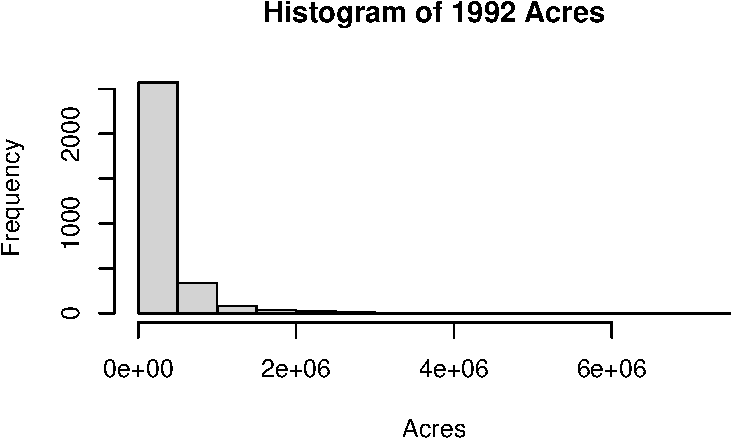
\includegraphics[keepaspectratio]{introR_files/figure-pdf/base-r-plots-1.pdf}}

\pandocbounded{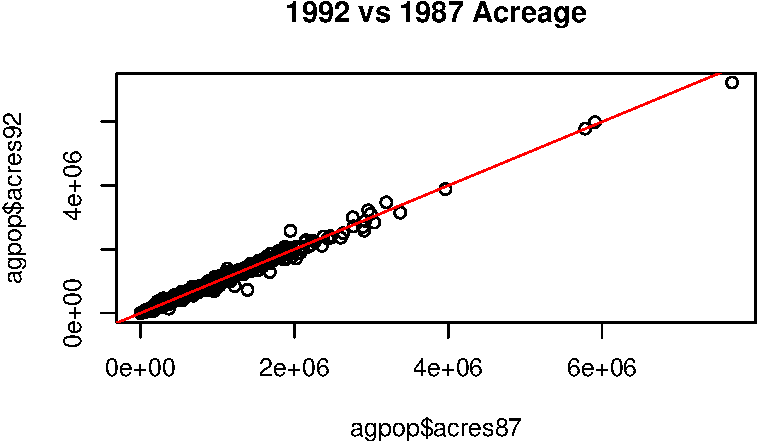
\includegraphics[keepaspectratio]{introR_files/figure-pdf/base-r-plots-2.pdf}}

Here is the new sub-section you can add right below your standard
plotting chunk to explain this workflow to your readers.

\subsection{Saving and Inserting External
Plots}\label{saving-and-inserting-external-plots}

Sometimes you need to export a high-resolution plot for a journal
submission or a presentation. You can save a plot directly to your
computer by opening a ``graphics device'' (like \texttt{pdf()},
\texttt{png()}, or \texttt{jpeg()}), running your plot code, and then
closing the device with \texttt{dev.off()}.

Once the file is saved in your project folder, you can insert it back
into your Quarto document at any time using the \texttt{knitr} package.

\begin{figure}[H]

{\centering 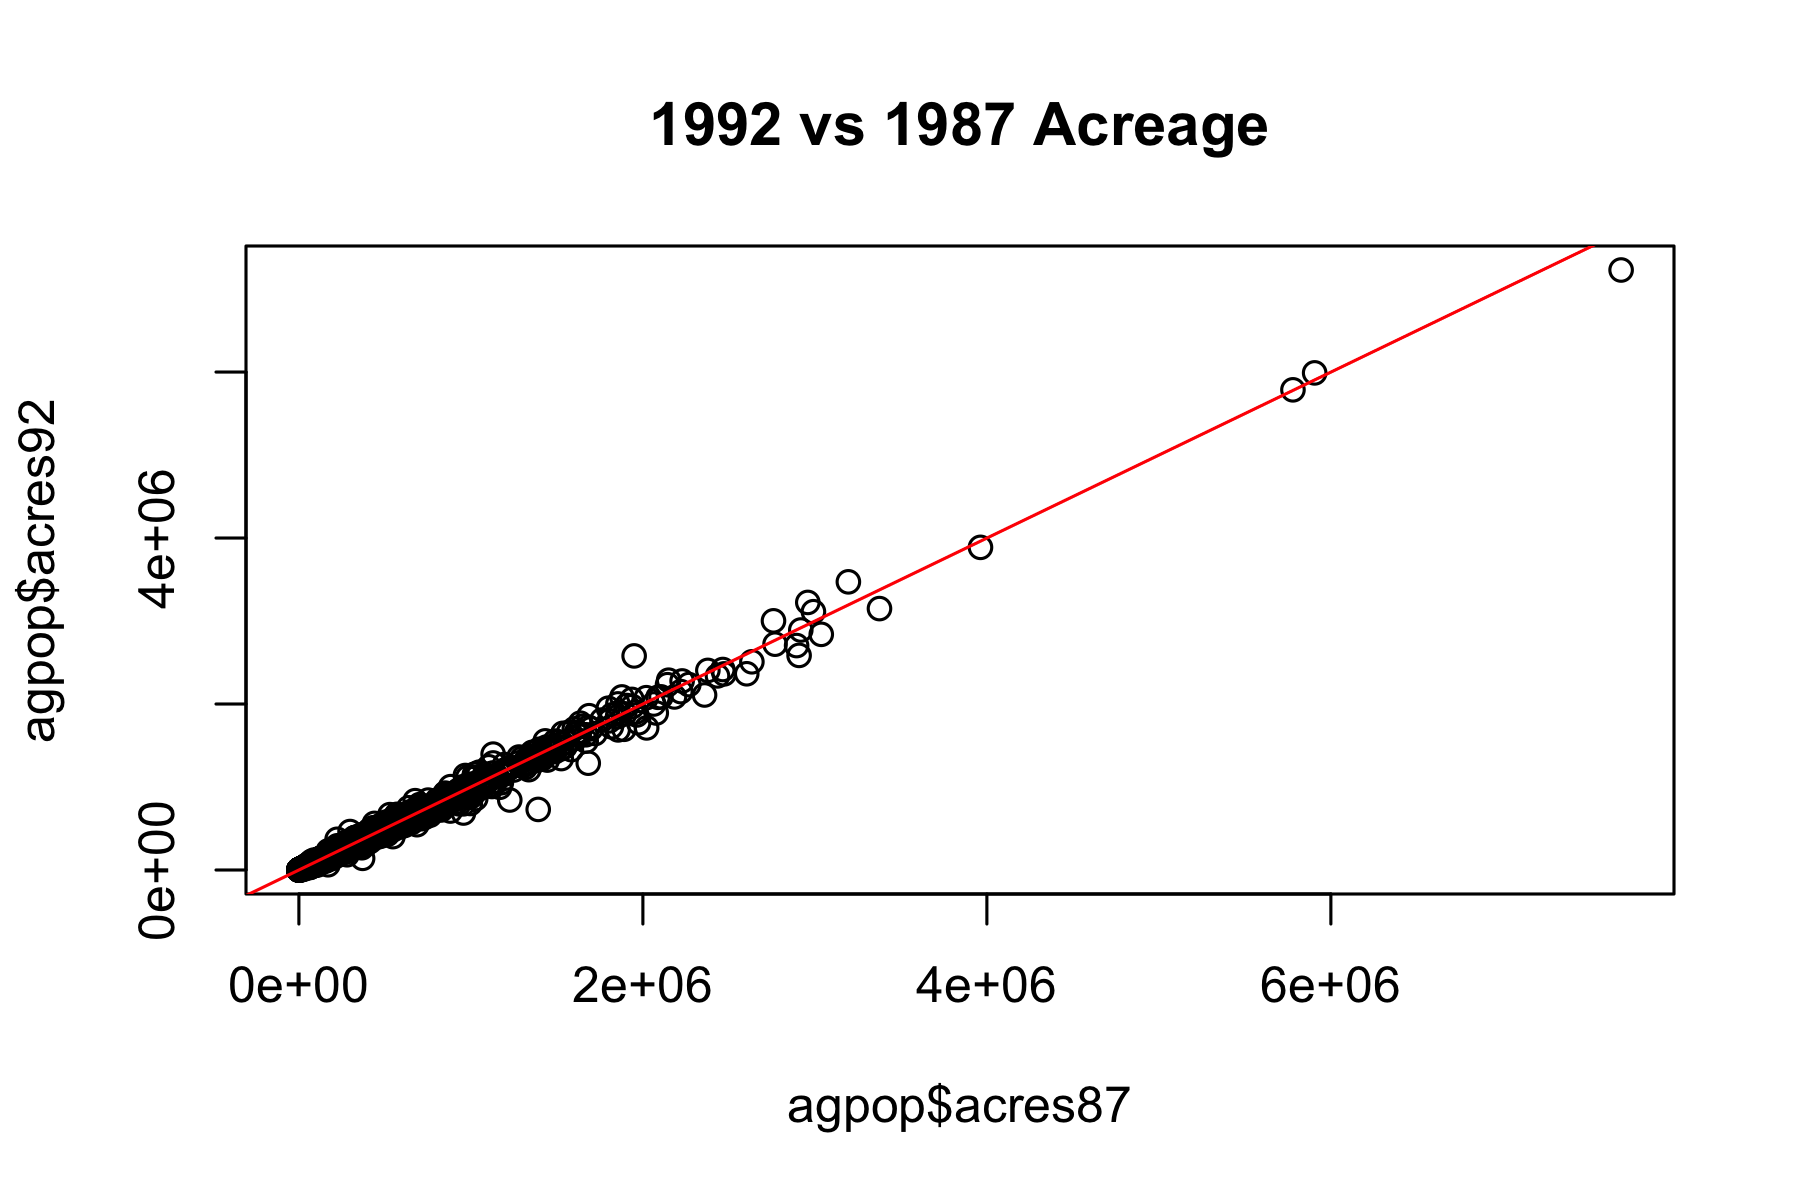
\includegraphics[width=6in,height=\textheight,keepaspectratio]{agpop_scatter_highres.png}

}

\caption{My Imported PNG Plot}

\end{figure}%

\subsection{\texorpdfstring{Advanced Visualization with
\texttt{ggplot2}}{Advanced Visualization with ggplot2}}\label{advanced-visualization-with-ggplot2}

While base R graphics are useful for quick checks, \texttt{ggplot2}
provides a powerful grammar of graphics for complex visuals. Below, we
generate a histogram of log-transformed 1992 acreages, overlaying both
an empirical density curve and a theoretical normal distribution curve.

\pandocbounded{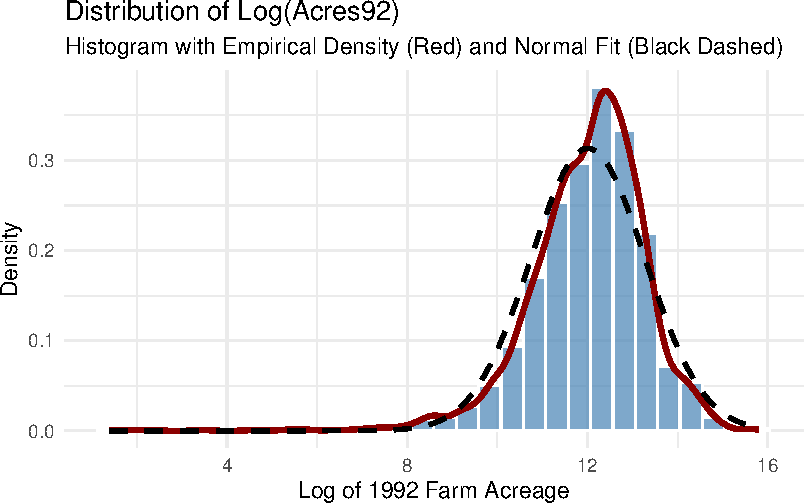
\includegraphics[keepaspectratio]{introR_files/figure-pdf/ggplot-histogram-1.pdf}}

\section{Create your own function}\label{create-your-own-function}

\begin{table}
\caption*{
{\fontsize{20}{25}\selectfont  Comparing Mean Calculations\fontsize{12}{15}\selectfont } \\ 
{\fontsize{14}{17}\selectfont  Custom Function vs. Base R colMeans()\fontsize{12}{15}\selectfont }
} 
\fontsize{12.0pt}{14.0pt}\selectfont
\begin{tabular*}{\linewidth}{@{\extracolsep{\fill}}lrr}
\toprule
\textbf{Variable} & \textbf{Custom \texttt{means\_col()}} & \textbf{Base \texttt{colMeans()}} \\ 
\midrule\addlinespace[2.5pt]
acres92 & 308,582.41 & 308,582.41 \\ 
acres87 & 315,373.71 & 315,373.71 \\ 
acres82 & 321,972.52 & 321,972.52 \\ 
farms92 & 625.50 & 625.50 \\ 
farms87 & 678.28 & 678.28 \\ 
farms82 & 728.06 & 728.06 \\ 
largef92 & 56.18 & 56.18 \\ 
largef87 & 54.86 & 54.86 \\ 
largef82 & 52.62 & 52.62 \\ 
smallf92 & 54.09 & 54.09 \\ 
smallf87 & 59.54 & 59.54 \\ 
\bottomrule
\end{tabular*}
\end{table}

\textbf{Output Note:} Displaying the results side-by-side confirms that
our custom \texttt{means\_col()} function produces the exact same output
as R's highly optimized built-in \texttt{colMeans()} function.

\bookmarksetup{startatroot}

\chapter{Simple Random Sampling}\label{simple-random-sampling}

\section{Analysis of agsrs.csv Data}\label{analysis-of-agsrs.csv-data}

\subsection{Step by step calculation without using a
function}\label{step-by-step-calculation-without-using-a-function}

To evaluate a Simple Random Sample (SRS), we calculate the point
estimate, the standard error (incorporating the Finite Population
Correction factor), and the margin of error to construct a 95\%
confidence interval.

\textbf{Key Formulas:}

\begin{itemize}
\tightlist
\item
  \textbf{Sample Mean:} \(\bar{y} = \frac{1}{n} \sum_{i=1}^n y_i\)
\item
  \textbf{Standard Error:}
  \(\mathrm{SE}(\bar{y}) = \sqrt{1 - \frac{n}{N}} \left( \frac{s}{\sqrt{n}} \right)\)
\item
  \textbf{Margin of Error:}
  \(\mathrm{ME} = t_{\alpha/2, n-1} \times \mathrm{SE}(\bar{y})\)
\item
  \textbf{Population Total:} \(\hat{t} = N\bar{y}\)
\end{itemize}

\begin{verbatim}
             county state acres92 acres87 acres82 farms92 farms87 farms82
1     COFFEE COUNTY    AL  175209  179311  194509     760     842     944
2    COLBERT COUNTY    AL  138135  145104  161360     488     563     686
3      LAMAR COUNTY    AL   56102   59861   72334     299     362     447
4    MARENGO COUNTY    AL  199117  220526  231207     434     471     622
5     MARION COUNTY    AL   89228  105586  113618     566     658     748
6 TUSCALOOSA COUNTY    AL   96194  120542  134616     436     521     650
  largef92 largef87 largef82 smallf92 smallf87 smallf82 region
1       29       28       21       57       47       66      S
2       37       41       42       12       44       47      S
3        4        4        3       16       20       30      S
4       48       66       62       14       11       28      S
5        7        9        9       11       23       27      S
6       20       17       23       18       32       29      S
\end{verbatim}

\begin{verbatim}
     Est.      S.E.    ci.low    ci.upp 
297897.05  18898.43 260706.26 335087.84 
\end{verbatim}

\begin{verbatim}
      Est.       S.E.     ci.low     ci.upp 
 916927110   58169381  802453859 1031400361 
\end{verbatim}

\subsection{Write a function for repeated
use}\label{write-a-function-for-repeated-use}

\subsubsection{A function for doing data analysis for srs
sample}\label{a-function-for-doing-data-analysis-for-srs-sample}

Wrap the previous manual calculations into a custom R function to
quickly estimate means, standard errors, and confidence intervals for
any variable of interest. To avoid repeating this code in every chapter,
all estimating functions (and their \texttt{gt}-table formatting
helpers) live in a single shared file, \texttt{samplingestimate.r},
which we source below.

\subsubsection{Apply srs\_est to agsrs.csv
data}\label{apply-srs_est-to-agsrs.csv-data}

\emph{Import Data}

Load the survey sample data representing US counties.

\emph{Estimating the mean of acre92}

Calculate the estimated average farm acreage per county using the custom
function. The function's \texttt{\$table} shows the row-level working
values (truncated to the first 6 rows + Sum), and \texttt{\$estimate}
holds the final point estimate, SE, and CI, formatted with
\texttt{format\_est\_gt()}.

\begin{table}
\caption*{
{\fontsize{20}{25}\selectfont  SRS Mean Estimation: Working Table\fontsize{12}{15}\selectfont } \\ 
{\fontsize{14}{17}\selectfont  \(n = 300\)\fontsize{12}{15}\selectfont }
} 
\fontsize{12.0pt}{14.0pt}\selectfont
\begin{tabular*}{\linewidth}{@{\extracolsep{\fill}}>{\raggedright\arraybackslash}p{\dimexpr 30.00pt -2\tabcolsep-1.5\arrayrulewidth}>{\raggedleft\arraybackslash}p{\dimexpr 82.50pt -2\tabcolsep-1.5\arrayrulewidth}>{\raggedleft\arraybackslash}p{\dimexpr 82.50pt -2\tabcolsep-1.5\arrayrulewidth}>{\raggedleft\arraybackslash}p{\dimexpr 82.50pt -2\tabcolsep-1.5\arrayrulewidth}}
\toprule
\(i\) & \(y_i\) & \(y_i-\bar y\) & \((y_i-\bar y)^2\)\textsuperscript{\textit{1}} \\ 
\midrule\addlinespace[2.5pt]
1 & 1.752 $\times$ 10\textsuperscript{5} & -1.227 $\times$ 10\textsuperscript{5} & 1.505 $\times$ 10\textsuperscript{10} \\ 
2 & 1.381 $\times$ 10\textsuperscript{5} & -1.598 $\times$ 10\textsuperscript{5} & 2.552 $\times$ 10\textsuperscript{10} \\ 
3 & 5.610 $\times$ 10\textsuperscript{4} & -2.418 $\times$ 10\textsuperscript{5} & 5.846 $\times$ 10\textsuperscript{10} \\ 
4 & 1.991 $\times$ 10\textsuperscript{5} & -9.878 $\times$ 10\textsuperscript{4} & 9.757 $\times$ 10\textsuperscript{9} \\ 
5 & 8.923 $\times$ 10\textsuperscript{4} & -2.087 $\times$ 10\textsuperscript{5} & 4.354 $\times$ 10\textsuperscript{10} \\ 
6 & 9.619 $\times$ 10\textsuperscript{4} & -2.017 $\times$ 10\textsuperscript{5} & 4.068 $\times$ 10\textsuperscript{10} \\ 
... & ... & ... & ... \\ 
{\bfseries Sum} & {\bfseries 8.937 $\times$ 10\textsuperscript{7}} & {\bfseries -3.900 $\times$ 10\textsuperscript{-8}} & {\bfseries 3.550 $\times$ 10\textsuperscript{13}} \\ 
\bottomrule
\end{tabular*}
\begin{minipage}{\linewidth}
\vspace{.05em}
\textsuperscript{\textit{1}}\(s_y^2 = \sum_i (y_i-\bar y)^2/(n-1) = 118716008180.4059\).\\
\textbf{Point estimate:} \(\bar y = \dfrac{\sum_i y_i}{n} = \dfrac{8.937 \times 10^{7}}{300} = 2.979 \times 10^{5}\)\\
\textbf{Standard error:} \(\mathrm{SE}(\bar y) = \sqrt{1-\dfrac{n}{N}}\,\dfrac{s}{\sqrt n} = \sqrt{1-\dfrac{300}{3078}}\,\dfrac{3.446 \times 10^{5}}{\sqrt{300}} = 18,898.434\)\\
\end{minipage}
\end{table}

\begin{table}
\fontsize{12.0pt}{14.0pt}\selectfont
\begin{tabular*}{0.7\linewidth}{@{\extracolsep{\fill}}rrrr}
\toprule
\(\bar{y}\) & \(\mathrm{SE}(\bar{y})\) & 95\% CI Lower & 95\% CI Upper \\ 
\midrule\addlinespace[2.5pt]
297,897.0467 & 18,898.4344 & 260,706.2569 & 335,087.8365 \\ 
\bottomrule
\end{tabular*}
\end{table}

\emph{Estimating the total of acre92}

Set \texttt{estimate\ =\ "total"} to have the function itself scale the
mean and confidence interval by the population size (\(N = 3078\)) to
estimate the total farm acreage across all counties.

\begin{table}
\fontsize{12.0pt}{14.0pt}\selectfont
\begin{tabular*}{0.7\linewidth}{@{\extracolsep{\fill}}rrrr}
\toprule
\(\hat{t}\) & \(\mathrm{SE}(\hat{t})\) & 95\% CI Lower & 95\% CI Upper \\ 
\midrule\addlinespace[2.5pt]
916,927,109.6400 & 58,169,381.1695 & 802,453,858.6054 & 1,031,400,360.6746 \\ 
\bottomrule
\end{tabular*}
\end{table}

\emph{Estimating the proportion of counties with fewer than 200K acres
for farming in 1992}

To estimate a proportion under SRS, create an indicator variable
(\(y_i = 1\) if true, \(0\) if false). The mean of this indicator
variable serves as the sample proportion
(\(\hat{p} = \bar{y}_{indicator}\)).

\begin{verbatim}
[1] 1 1 1 1 1 1
\end{verbatim}

\begin{table}
\fontsize{12.0pt}{14.0pt}\selectfont
\begin{tabular*}{0.7\linewidth}{@{\extracolsep{\fill}}rrrr}
\toprule
\(\bar{y}\) & \(\mathrm{SE}(\bar{y})\) & 95\% CI Lower & 95\% CI Upper \\ 
\midrule\addlinespace[2.5pt]
0.5100 & 0.0275 & 0.4560 & 0.5640 \\ 
\bottomrule
\end{tabular*}
\end{table}

\emph{Estimating the total number of counties with fewer than 200K acres
for farming in 1992}

Set \texttt{estimate\ =\ "total"} to estimate the absolute count of
counties meeting the criteria.

\begin{table}
\fontsize{12.0pt}{14.0pt}\selectfont
\begin{tabular*}{0.7\linewidth}{@{\extracolsep{\fill}}rrrr}
\toprule
\(\hat{t}\) & \(\mathrm{SE}(\hat{t})\) & 95\% CI Lower & 95\% CI Upper \\ 
\midrule\addlinespace[2.5pt]
1,569.7800 & 84.5372 & 1,403.4167 & 1,736.1433 \\ 
\bottomrule
\end{tabular*}
\end{table}

\subsection{Comparing with true value}\label{comparing-with-true-value}

Load the complete census (population) dataset to calculate the true
parameters. This allows us to assess the accuracy of our previous SRS
estimates against the exact population values.

\begin{verbatim}
[1] 308582.4
\end{verbatim}

\begin{verbatim}
[1] 943953599
\end{verbatim}

\begin{verbatim}
[1] 0.5145472
\end{verbatim}

\begin{verbatim}
[1] 1574
\end{verbatim}

\section{A Simulation Demonstration of SRS
Inference}\label{a-simulation-demonstration-of-srs-inference}

Load the full population data and filter out missing values to serve as
a complete, known finite population for resampling experiments.

\subsection{True Values}\label{true-values}

Define the target sample size and compute the true population mean
(\(\mu\)) and theoretical standard error (\(\mathrm{SE}_{true}\)) using
the known population standard deviation (\(S\)).

\textbf{Theoretical Standard Error:}

\[\mathrm{SE}_{true}(\bar{y}) = \sqrt{1 - \frac{n}{N}} \left(\frac{S}{\sqrt{n}}\right)\]

\begin{verbatim}
[1] 3059
\end{verbatim}

\begin{verbatim}
[1] 308582.4
\end{verbatim}

\begin{verbatim}
[1] 23320.29
\end{verbatim}

\subsection{One SRS sampling}\label{one-srs-sampling}

Draw a single random sample of size \(n=300\) from the population and
run our estimator function to see a single instance of survey inference.

\begin{verbatim}
                county state acres92 acres87 acres82 farms92 farms87 farms82
463      MONROE COUNTY    GA   44599   39407   58630     179     160     172
3       FAIRBANKS AREA    AK  141338  154913  204568     168     175     170
2921    SPOKANE COUNTY    WA  625769  613055  626780    1708    1901    2193
1102    DE SOTO PARISH    LA  147826  154522  166066     556     585     679
2881   FRANKLIN COUNTY    VT  203503  214344  223560     728     786     795
2868 WASHINGTON COUNTY    VA  190062  202709  215393    1986    1972    2289
     largef92 largef87 largef82 smallf92 smallf87 smallf82 region
463         5        7        9       12        9       11      S
3          25       28       21       12       18       25      W
2921      190      171      168      197      224      300      W
1102       33       26       32       26       30       44      S
2881       13       14       11       24       35       30     NE
2868       15       17       13      380      325      412      S
\end{verbatim}

\begin{table}
\fontsize{12.0pt}{14.0pt}\selectfont
\begin{tabular*}{0.7\linewidth}{@{\extracolsep{\fill}}rrrr}
\toprule
\(\bar{y}\) & \(\mathrm{SE}(\bar{y})\) & 95\% CI Lower & 95\% CI Upper \\ 
\midrule\addlinespace[2.5pt]
290,384.6600 & 22,626.9559 & 245,856.4021 & 334,912.9179 \\ 
\bottomrule
\end{tabular*}
\end{table}

\subsection{Repeating SRS sampling 5000
times}\label{repeating-srs-sampling-5000-times}

To demonstrate the Central Limit Theorem and unbiasedness of the
estimator, draw 5,000 independent samples, storing the estimates from
each iteration. We plot the resulting sampling distribution against the
true population mean.

\emph{(Note: We use \texttt{show.details\ =\ FALSE} and pull out just
\texttt{\$estimate} here, so the loop skips building 5,000 working
tables and stays fast.)}

\begin{verbatim}
         Est.     S.E.   ci.low   ci.upp
[1,] 329001.3 24062.86 281647.3 376355.3
[2,] 318260.5 22819.01 273354.3 363166.7
[3,] 318198.8 29725.16 259701.8 376695.8
[4,] 332783.3 22275.51 288946.7 376619.9
[5,] 293297.0 19405.03 255109.3 331484.8
[6,] 268717.9 14164.38 240843.4 296592.4
\end{verbatim}

\pandocbounded{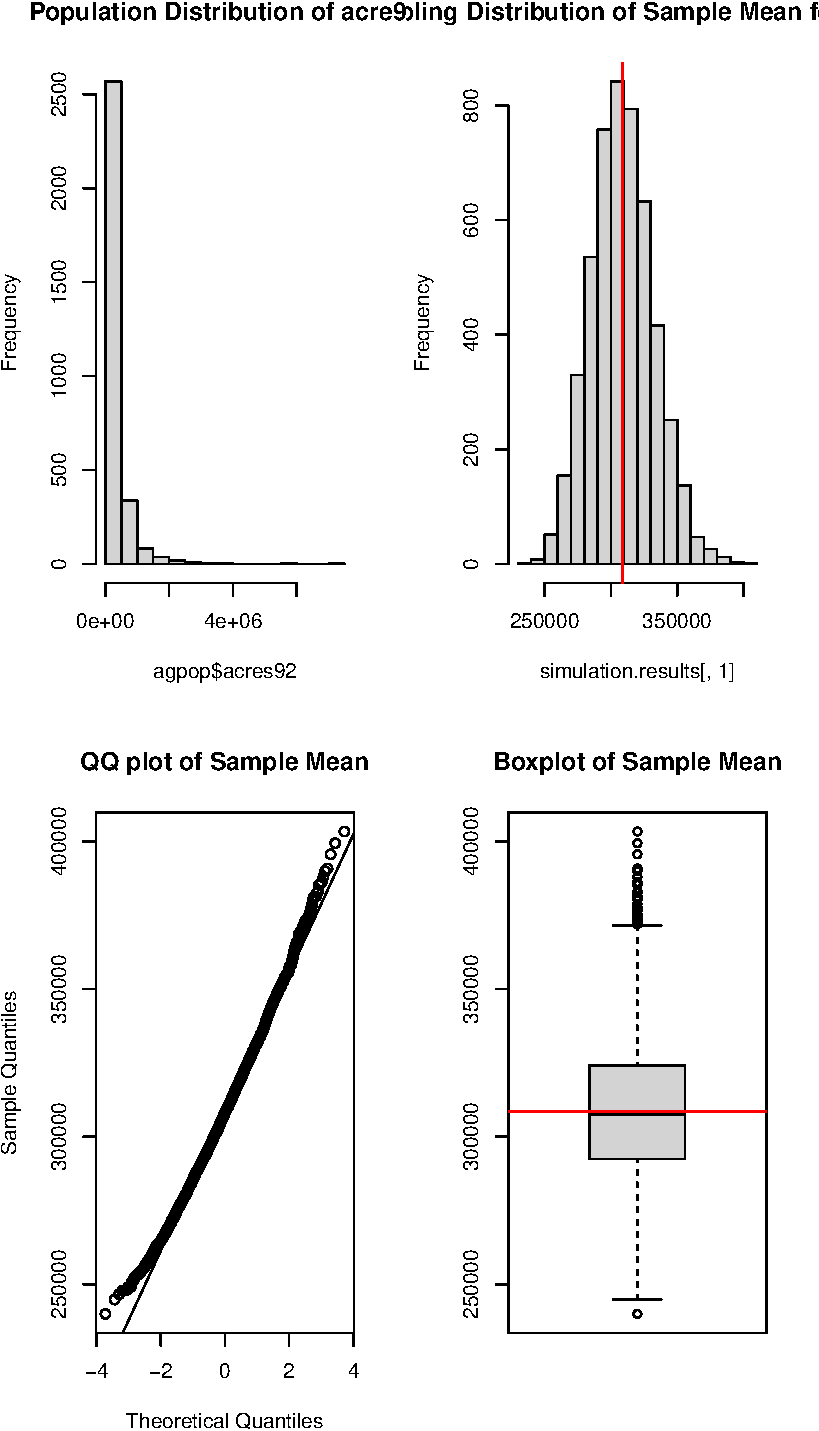
\includegraphics[keepaspectratio]{srs_files/figure-pdf/srs-simulation-1.pdf}}

\begin{verbatim}
[1] 308734.1
\end{verbatim}

\begin{verbatim}
[1] 308582.4
\end{verbatim}

\begin{verbatim}
[1] 23371.27
\end{verbatim}

\begin{verbatim}
[1] 23320.29
\end{verbatim}

\subsection{Empirical Coverage Rate of
CIs}\label{empirical-coverage-rate-of-cis}

Verify the reliability of the 95\% confidence intervals by checking
whether the true population mean falls within the calculated bounds for
each of the 5,000 samples. The empirical coverage rate should closely
approximate 0.95. The plot highlights the first 100 intervals, flagging
those that fail to capture the true mean in a distinct color.

\begin{verbatim}
      Est.     S.E.   ci.low   ci.upp Covered?
1 329001.3 24062.86 281647.3 376355.3        1
2 318260.5 22819.01 273354.3 363166.7        1
3 318198.8 29725.16 259701.8 376695.8        1
4 332783.3 22275.51 288946.7 376619.9        1
5 293297.0 19405.03 255109.3 331484.8        1
6 268717.9 14164.38 240843.4 296592.4        0
\end{verbatim}

\pandocbounded{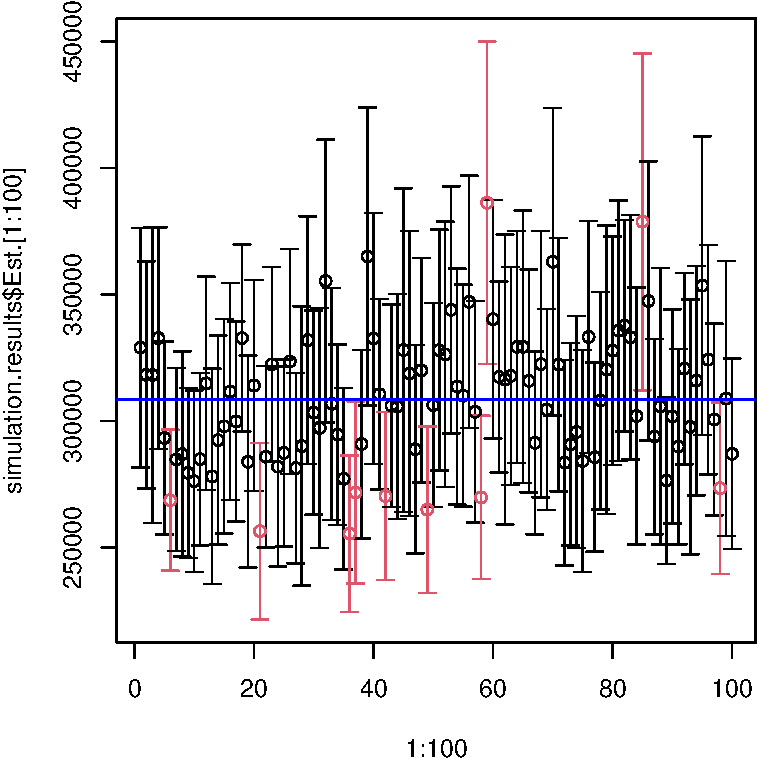
\includegraphics[keepaspectratio]{srs_files/figure-pdf/srs-coverage-1.pdf}}

\begin{verbatim}
[1] 0.931
\end{verbatim}

\bookmarksetup{startatroot}

\chapter{Stratified Random Sampling}\label{stratified-random-sampling}

\section{Key Formulas for Stratified
Sampling}\label{key-formulas-for-stratified-sampling}

Stratified random sampling divides a population of size \(N\) into \(H\)
mutually exclusive strata. A simple random sample of size \(n_h\) is
then drawn from each stratum of size \(N_h\). This design often yields
higher precision than Simple Random Sampling (SRS).

\subsubsection*{1. Stratified Population Mean
Estimator}\label{stratified-population-mean-estimator}
\addcontentsline{toc}{subsubsection}{1. Stratified Population Mean
Estimator}

The estimated population mean is a weighted average of the sample means
from each stratum: \[
\overline{y}_{str} = \sum_{h=1}^H \pi_h \overline{y}_h.
\] Where \(\pi_h = \frac{N_h}{N}\) is the stratum weight, and
\(\overline{y}_h\) is the sample mean of stratum \(h\).

\subsubsection*{2. Variance of the Stratified
Mean}\label{variance-of-the-stratified-mean}
\addcontentsline{toc}{subsubsection}{2. Variance of the Stratified Mean}

The estimated variance accounts for the finite population correction in
each stratum: \[
\hat{V}(\overline{y}_{str}) = \sum_{h=1}^H \pi_h^2 \left(1 - \frac{n_h}{N_h}\right) \frac{s_h^2}{n_h}.
\] Where \(s_h^2\) is the sample variance in stratum \(h\).

\subsubsection*{3. Proportional
Allocation}\label{proportional-allocation}
\addcontentsline{toc}{subsubsection}{3. Proportional Allocation}

Sample sizes are allocated proportional to the size of the stratum: \[
n_h = n \left( \frac{N_h}{N} \right).
\]

\subsubsection*{4. Neyman (Optimal)
Allocation}\label{neyman-optimal-allocation}
\addcontentsline{toc}{subsubsection}{4. Neyman (Optimal) Allocation}

If surveying costs are equal across strata, Neyman allocation minimizes
the variance of the estimator by sampling more heavily from larger and
more highly variable strata: \[
n_h = n \frac{N_h S_h}{\sum_{h=1}^H N_h S_h}
\]

\begin{center}\rule{0.5\linewidth}{0.5pt}\end{center}

\section{Functions and packages for Analyzing
Data}\label{functions-and-packages-for-analyzing-data}

The estimating functions used throughout this book (including
\texttt{str\_est}, \texttt{str\_est\_data}, and \texttt{srs\_est}, used
below to compute the stratified mean, standard error, and confidence
intervals) live in a single shared file, \texttt{samplingestimate.r},
which we source below. \texttt{str\_est\_data} computes these directly
from a dataset, while \texttt{str\_est} computes them from
pre-calculated summary statistics.

\section{Analysis of ``agstrat.csv''
data}\label{analysis-of-agstrat.csv-data}

We will estimate the average 1992 farm acreage (\texttt{acres92}) across
US counties, using geographic region (\texttt{region}) as the
stratification variable.

\subsection{Importing agstrat.csv
data}\label{importing-agstrat.csv-data}

\begin{table}
\fontsize{12.0pt}{14.0pt}\selectfont
\begin{tabular*}{\linewidth}{@{\extracolsep{\fill}}llrrrrrrrrrrrrlrr}
\toprule
county & state & acres92 & acres87 & acres82 & farms92 & farms87 & farms82 & largef92 & largef87 & largef82 & smallf92 & smallf87 & smallf82 & region & rn & weight \\ 
\midrule\addlinespace[2.5pt]
PIERCE COUNTY & NE & 297326 & 332862 & 319619 & 725 & 857 & 865 & 54 & 54 & 42 & 58 & 67 & 48 & NC & 805 & 10.23301 \\ 
JENNINGS COUNTY & IN & 124694 & 131481 & 139111 & 658 & 671 & 751 & 14 & 13 & 14 & 42 & 36 & 38 & NC & 241 & 10.23301 \\ 
WAYNE COUNTY & OH & 246938 & 263457 & 268434 & 1582 & 1734 & 1866 & 20 & 19 & 16 & 175 & 186 & 184 & NC & 913 & 10.23301 \\ 
VAN BUREN COUNTY & MI & 206781 & 190251 & 197055 & 1164 & 1278 & 1464 & 23 & 17 & 9 & 56 & 66 & 55 & NC & 478 & 10.23301 \\ 
OZAUKEE COUNTY & WI & 78772 & 85201 & 89331 & 448 & 483 & 527 & 6 & 5 & 5 & 56 & 49 & 48 & NC & 1028 & 10.23301 \\ 
CLEARWATER COUNTY & MN & 210897 & 229537 & 213105 & 583 & 699 & 693 & 34 & 32 & 23 & 8 & 19 & 13 & NC & 496 & 10.23301 \\ 
\bottomrule
\end{tabular*}
\end{table}

\textbf{Output Note:} The table above shows the sample survey data,
including the stratum (region) and weights for each county.

\subsection{Spreadsheet calculation}\label{spreadsheet-calculation}

\subsubsection{Summarizing acre92 in each
stratum}\label{summarizing-acre92-in-each-stratum}

We first manually compute the sample size (\(n_h\)), standard deviation
(\(s_h\)), and mean (\(\overline{y}_h\)) for each region, matching them
with the known total counties in each region (\(N_h\)).

\begin{table}
\fontsize{12.0pt}{14.0pt}\selectfont
\begin{tabular*}{\linewidth}{@{\extracolsep{\fill}}l|rrrr}
\toprule
 & \(N_h\) & \(n_h\) & \(\bar{y}_h\) & \(s_h\) \\ 
\midrule\addlinespace[2.5pt]
NC & 1054 & 103 & 300,504.16 & 172,099.34 \\ 
NE & 220 & 21 & 97,629.81 & 87,449.83 \\ 
S & 1382 & 135 & 211,315.04 & 231,489.71 \\ 
W & 422 & 41 & 662,295.51 & 629,433.04 \\ 
\bottomrule
\end{tabular*}
\end{table}

\textbf{Output Note:} This displays the summary statistics per stratum.
Note the significantly high variance (\(s_h\)) in the W region compared
to the others.

\subsubsection{Estimates}\label{estimates}

Rather than building the ``spreadsheet-style'' working table by hand, we
call \texttt{str\_est()}, whose \texttt{\$table} shows the same
intermediate stratum-level values (\(N_h\), \(n_h\), \(\pi_h\),
\(\bar y_h\), \(s_h^2\), \(\pi_h\bar y_h\), \(v_h\)) needed for the
final stratified mean and variance, with a Total row and footnotes for
\(\pi_h\) and \(v_h\).

\begin{table}
\caption*{
{\fontsize{20}{25}\selectfont  Stratified Mean Estimation: Working Table\fontsize{12}{15}\selectfont }
} 
\fontsize{12.0pt}{14.0pt}\selectfont
\begin{tabular*}{\linewidth}{@{\extracolsep{\fill}}>{\raggedright\arraybackslash}p{\dimexpr 82.50pt -2\tabcolsep-1.5\arrayrulewidth}>{\raggedleft\arraybackslash}p{\dimexpr 45.00pt -2\tabcolsep-1.5\arrayrulewidth}>{\raggedleft\arraybackslash}p{\dimexpr 45.00pt -2\tabcolsep-1.5\arrayrulewidth}>{\raggedleft\arraybackslash}p{\dimexpr 82.50pt -2\tabcolsep-1.5\arrayrulewidth}>{\raggedleft\arraybackslash}p{\dimexpr 82.50pt -2\tabcolsep-1.5\arrayrulewidth}>{\raggedleft\arraybackslash}p{\dimexpr 82.50pt -2\tabcolsep-1.5\arrayrulewidth}>{\raggedleft\arraybackslash}p{\dimexpr 82.50pt -2\tabcolsep-1.5\arrayrulewidth}>{\raggedleft\arraybackslash}p{\dimexpr 82.50pt -2\tabcolsep-1.5\arrayrulewidth}}
\toprule
Stratum & \(N_h\) & \(n_h\) & \(\pi_h\)\textsuperscript{\textit{1}} & \(\bar y_h\) & \(s_h^2\) & \(\pi_h\bar y_h\) & \(v_h\)\textsuperscript{\textit{2}} \\ 
\midrule\addlinespace[2.5pt]
NC & 1,054 & 103 & 0.34 & 3.01 $\times$ 10\textsuperscript{5} & 2.96 $\times$ 10\textsuperscript{10} & 1.03 $\times$ 10\textsuperscript{5} & 3.04 $\times$ 10\textsuperscript{7} \\ 
NE & 220 & 21 & 0.07 & 9.76 $\times$ 10\textsuperscript{4} & 7.65 $\times$ 10\textsuperscript{9} & 6.98 $\times$ 10\textsuperscript{3} & 1.68 $\times$ 10\textsuperscript{6} \\ 
S & 1,382 & 135 & 0.45 & 2.11 $\times$ 10\textsuperscript{5} & 5.36 $\times$ 10\textsuperscript{10} & 9.49 $\times$ 10\textsuperscript{4} & 7.22 $\times$ 10\textsuperscript{7} \\ 
W & 422 & 41 & 0.14 & 6.62 $\times$ 10\textsuperscript{5} & 3.96 $\times$ 10\textsuperscript{11} & 9.08 $\times$ 10\textsuperscript{4} & 1.64 $\times$ 10\textsuperscript{8} \\ 
{\bfseries Total} & {\bfseries 3,078} & {\bfseries 300} & {\bfseries 1.00} & {\bfseries } & {\bfseries } & {\bfseries 2.96 $\times$ 10\textsuperscript{5}} & {\bfseries 2.68 $\times$ 10\textsuperscript{8}} \\ 
\bottomrule
\end{tabular*}
\begin{minipage}{\linewidth}
\vspace{.05em}
\textsuperscript{\textit{1}}\(\pi_h = N_h/N\) is the stratum weight.\\
\textsuperscript{\textit{2}}\(v_h = (1-n_h/N_h)\,\pi_h^2\, s_h^2/n_h\) is stratum \(h\)'s contribution to \(V(\bar y_{str}) = \sum_h v_h\).\\
\textbf{Point estimate:} \(\bar y_{str} = \sum_h \pi_h\bar y_h = 2.956 \times 10^{5}\)\\
\textbf{Standard error:} \(\mathrm{SE}(\bar y_{str}) = \sqrt{\sum_h v_h} = \sqrt{2.683 \times 10^{8}} = 16,379.873\)\\
\end{minipage}
\end{table}

\textbf{Output Note:} The table provides a detailed breakdown of how
each individual stratum contributes to the final mean and variance.

Extracting \texttt{\$estimate} gives our overall result.

\begin{table}
\fontsize{12.0pt}{14.0pt}\selectfont
\begin{tabular*}{0.7\linewidth}{@{\extracolsep{\fill}}rrrr}
\toprule
\(\bar{y}\) & \(\mathrm{SE}(\bar{y})\) & 95\% CI Lower & 95\% CI Upper \\ 
\midrule\addlinespace[2.5pt]
295,560.7652 & 16,379.8727 & 263,456.2147 & 327,665.3158 \\ 
\bottomrule
\end{tabular*}
\end{table}

\textbf{Output Note:} The overall result indicates an estimated mean of
295,561 acres, with a 95\% confidence interval of {[}263,456,
327,665{]}.

To find the population total (total acreage across all US counties), set
\texttt{estimate\ =\ "total"}.

\begin{table}
\fontsize{12.0pt}{14.0pt}\selectfont
\begin{tabular*}{0.7\linewidth}{@{\extracolsep{\fill}}rrrr}
\toprule
\(\hat{t}\) & \(\mathrm{SE}(\hat{t})\) & 95\% CI Lower & 95\% CI Upper \\ 
\midrule\addlinespace[2.5pt]
909,736,035.3920 & 50,417,248.2519 & 810,918,228.8183 & 1,008,553,841.9656 \\ 
\bottomrule
\end{tabular*}
\end{table}

\textbf{Output Note:} This scales the estimates up to the total area of
909,736,035 acres.

\subsection{Using the function
``str\_est\_data''}\label{using-the-function-str_est_data}

Instead of pre-calculating the summary stats, this function extracts
everything directly from the dataset using the pre-assigned sampling
weights.

\begin{verbatim}
  NC   NE    S    W 
1054  220 1382  422 
\end{verbatim}

\textbf{Output Note:} This reconstructs the total population sizes
(\(N_h\)) per region.

\begin{table}
\caption*{
{\fontsize{20}{25}\selectfont  Stratified Mean Estimation: Working Table\fontsize{12}{15}\selectfont }
} 
\fontsize{12.0pt}{14.0pt}\selectfont
\begin{tabular*}{\linewidth}{@{\extracolsep{\fill}}>{\raggedright\arraybackslash}p{\dimexpr 82.50pt -2\tabcolsep-1.5\arrayrulewidth}>{\raggedleft\arraybackslash}p{\dimexpr 45.00pt -2\tabcolsep-1.5\arrayrulewidth}>{\raggedleft\arraybackslash}p{\dimexpr 45.00pt -2\tabcolsep-1.5\arrayrulewidth}>{\raggedleft\arraybackslash}p{\dimexpr 82.50pt -2\tabcolsep-1.5\arrayrulewidth}>{\raggedleft\arraybackslash}p{\dimexpr 82.50pt -2\tabcolsep-1.5\arrayrulewidth}>{\raggedleft\arraybackslash}p{\dimexpr 82.50pt -2\tabcolsep-1.5\arrayrulewidth}>{\raggedleft\arraybackslash}p{\dimexpr 82.50pt -2\tabcolsep-1.5\arrayrulewidth}>{\raggedleft\arraybackslash}p{\dimexpr 82.50pt -2\tabcolsep-1.5\arrayrulewidth}}
\toprule
Stratum & \(N_h\) & \(n_h\) & \(\pi_h\)\textsuperscript{\textit{1}} & \(\bar y_h\) & \(s_h^2\) & \(\pi_h\bar y_h\) & \(v_h\)\textsuperscript{\textit{2}} \\ 
\midrule\addlinespace[2.5pt]
NC & 1,054 & 103 & 0.34 & 3.01 $\times$ 10\textsuperscript{5} & 2.96 $\times$ 10\textsuperscript{10} & 1.03 $\times$ 10\textsuperscript{5} & 3.04 $\times$ 10\textsuperscript{7} \\ 
NE & 220 & 21 & 0.07 & 9.76 $\times$ 10\textsuperscript{4} & 7.65 $\times$ 10\textsuperscript{9} & 6.98 $\times$ 10\textsuperscript{3} & 1.68 $\times$ 10\textsuperscript{6} \\ 
S & 1,382 & 135 & 0.45 & 2.11 $\times$ 10\textsuperscript{5} & 5.36 $\times$ 10\textsuperscript{10} & 9.49 $\times$ 10\textsuperscript{4} & 7.22 $\times$ 10\textsuperscript{7} \\ 
W & 422 & 41 & 0.14 & 6.62 $\times$ 10\textsuperscript{5} & 3.96 $\times$ 10\textsuperscript{11} & 9.08 $\times$ 10\textsuperscript{4} & 1.64 $\times$ 10\textsuperscript{8} \\ 
{\bfseries Total} & {\bfseries 3,078} & {\bfseries 300} & {\bfseries 1.00} & {\bfseries } & {\bfseries } & {\bfseries 2.96 $\times$ 10\textsuperscript{5}} & {\bfseries 2.68 $\times$ 10\textsuperscript{8}} \\ 
\bottomrule
\end{tabular*}
\begin{minipage}{\linewidth}
\vspace{.05em}
\textsuperscript{\textit{1}}\(\pi_h = N_h/N\) is the stratum weight.\\
\textsuperscript{\textit{2}}\(v_h = (1-n_h/N_h)\,\pi_h^2\, s_h^2/n_h\) is stratum \(h\)'s contribution to \(V(\bar y_{str}) = \sum_h v_h\).\\
\textbf{Point estimate:} \(\bar y_{str} = \sum_h \pi_h\bar y_h = 2.956 \times 10^{5}\)\\
\textbf{Standard error:} \(\mathrm{SE}(\bar y_{str}) = \sqrt{\sum_h v_h} = \sqrt{2.683 \times 10^{8}} = 16,379.873\)\\
\end{minipage}
\end{table}

\begin{table}
\fontsize{12.0pt}{14.0pt}\selectfont
\begin{tabular*}{0.7\linewidth}{@{\extracolsep{\fill}}rrrr}
\toprule
\(\bar{y}\) & \(\mathrm{SE}(\bar{y})\) & 95\% CI Lower & 95\% CI Upper \\ 
\midrule\addlinespace[2.5pt]
295,560.7652 & 16,379.8727 & 263,456.2147 & 327,665.3158 \\ 
\bottomrule
\end{tabular*}
\end{table}

\textbf{Output Note:} Once again, this perfectly matches the manual
calculation.

\begin{table}
\caption*{
{\fontsize{20}{25}\selectfont  Stratified Mean Estimation: Working Table\fontsize{12}{15}\selectfont }
} 
\fontsize{12.0pt}{14.0pt}\selectfont
\begin{tabular*}{\linewidth}{@{\extracolsep{\fill}}>{\raggedright\arraybackslash}p{\dimexpr 82.50pt -2\tabcolsep-1.5\arrayrulewidth}>{\raggedleft\arraybackslash}p{\dimexpr 45.00pt -2\tabcolsep-1.5\arrayrulewidth}>{\raggedleft\arraybackslash}p{\dimexpr 45.00pt -2\tabcolsep-1.5\arrayrulewidth}>{\raggedleft\arraybackslash}p{\dimexpr 82.50pt -2\tabcolsep-1.5\arrayrulewidth}>{\raggedleft\arraybackslash}p{\dimexpr 82.50pt -2\tabcolsep-1.5\arrayrulewidth}>{\raggedleft\arraybackslash}p{\dimexpr 82.50pt -2\tabcolsep-1.5\arrayrulewidth}>{\raggedleft\arraybackslash}p{\dimexpr 82.50pt -2\tabcolsep-1.5\arrayrulewidth}>{\raggedleft\arraybackslash}p{\dimexpr 82.50pt -2\tabcolsep-1.5\arrayrulewidth}}
\toprule
Stratum & \(N_h\) & \(n_h\) & \(\pi_h\)\textsuperscript{\textit{1}} & \(\bar y_h\) & \(s_h^2\) & \(\pi_h\bar y_h\) & \(v_h\)\textsuperscript{\textit{2}} \\ 
\midrule\addlinespace[2.5pt]
NC & 1,054 & 103 & 0.34 & 44.26 & 1.29 $\times$ 10\textsuperscript{3} & 15.16 & 1.32 \\ 
NE & 220 & 21 & 0.07 & 47.24 & 2.36 $\times$ 10\textsuperscript{3} & 3.38 & 0.52 \\ 
S & 1,382 & 135 & 0.45 & 47.39 & 6.21 $\times$ 10\textsuperscript{3} & 21.28 & 8.36 \\ 
W & 422 & 41 & 0.14 & 124.39 & 1.01 $\times$ 10\textsuperscript{5} & 17.05 & 41.66 \\ 
{\bfseries Total} & {\bfseries 3,078} & {\bfseries 300} & {\bfseries 1.00} & {\bfseries } & {\bfseries } & {\bfseries 56.86} & {\bfseries 51.86} \\ 
\bottomrule
\end{tabular*}
\begin{minipage}{\linewidth}
\vspace{.05em}
\textsuperscript{\textit{1}}\(\pi_h = N_h/N\) is the stratum weight.\\
\textsuperscript{\textit{2}}\(v_h = (1-n_h/N_h)\,\pi_h^2\, s_h^2/n_h\) is stratum \(h\)'s contribution to \(V(\bar y_{str}) = \sum_h v_h\).\\
\textbf{Point estimate:} \(\bar y_{str} = \sum_h \pi_h\bar y_h = 56.863\)\\
\textbf{Standard error:} \(\mathrm{SE}(\bar y_{str}) = \sqrt{\sum_h v_h} = \sqrt{51.860} = 7.201\)\\
\end{minipage}
\end{table}

\begin{table}
\fontsize{12.0pt}{14.0pt}\selectfont
\begin{tabular*}{0.7\linewidth}{@{\extracolsep{\fill}}rrrr}
\toprule
\(\bar{y}\) & \(\mathrm{SE}(\bar{y})\) & 95\% CI Lower & 95\% CI Upper \\ 
\midrule\addlinespace[2.5pt]
56.8628 & 7.2014 & 42.7480 & 70.9776 \\ 
\bottomrule
\end{tabular*}
\end{table}

\textbf{Output Note:} This demonstrates the function's flexibility: we
can easily estimate a different variable (an average of 56.9 small farms
per county).

\subsection{Comparing with SRS
estimate}\label{comparing-with-srs-estimate}

To see the benefit of stratifying, we compare our stratified estimates
against a Simple Random Sample approach on the same population.

\begin{table}
\fontsize{12.0pt}{14.0pt}\selectfont
\begin{tabular*}{0.7\linewidth}{@{\extracolsep{\fill}}rrrr}
\toprule
\(\bar{y}\) & \(\mathrm{SE}(\bar{y})\) & 95\% CI Lower & 95\% CI Upper \\ 
\midrule\addlinespace[2.5pt]
297,897.0467 & 18,898.4344 & 260,706.2569 & 335,087.8365 \\ 
\bottomrule
\end{tabular*}
\end{table}

\textbf{Output Note:} The Simple Random Sample standard error is
noticeably higher at 18,898.

\begin{verbatim}
[1] 0.7512239
\end{verbatim}

\textbf{Output Note:} The stratified variance is approximately 75.1\% of
the SRS variance.

\begin{verbatim}
[1] 0.2487761
\end{verbatim}

\textbf{Output Note:} Stratification by region reduced the variance by
24.9\%. This is a substantial gain in precision for no extra sampling
cost.

\section{Allocation of stratum sample
size}\label{allocation-of-stratum-sample-size}

Deciding how to distribute the total sample \(n\) among the strata
significantly impacts the precision of the estimator.

\subsection{Analyzing seals.csv collected with stratified
sampling}\label{analyzing-seals.csv-collected-with-stratified-sampling}

This dataset investigates ringed seal holes in different zones. The
researchers used Proportional Allocation, taking 20\% of the areas in
each zone.

\begin{table}
\caption*{
{\fontsize{20}{25}\selectfont  Stratified Mean Estimation: Working Table\fontsize{12}{15}\selectfont }
} 
\fontsize{12.0pt}{14.0pt}\selectfont
\begin{tabular*}{\linewidth}{@{\extracolsep{\fill}}>{\raggedright\arraybackslash}p{\dimexpr 82.50pt -2\tabcolsep-1.5\arrayrulewidth}>{\raggedleft\arraybackslash}p{\dimexpr 45.00pt -2\tabcolsep-1.5\arrayrulewidth}>{\raggedleft\arraybackslash}p{\dimexpr 45.00pt -2\tabcolsep-1.5\arrayrulewidth}>{\raggedleft\arraybackslash}p{\dimexpr 82.50pt -2\tabcolsep-1.5\arrayrulewidth}>{\raggedleft\arraybackslash}p{\dimexpr 82.50pt -2\tabcolsep-1.5\arrayrulewidth}>{\raggedleft\arraybackslash}p{\dimexpr 82.50pt -2\tabcolsep-1.5\arrayrulewidth}>{\raggedleft\arraybackslash}p{\dimexpr 82.50pt -2\tabcolsep-1.5\arrayrulewidth}>{\raggedleft\arraybackslash}p{\dimexpr 82.50pt -2\tabcolsep-1.5\arrayrulewidth}}
\toprule
Stratum & \(N_h\) & \(n_h\) & \(\pi_h\)\textsuperscript{\textit{1}} & \(\bar y_h\) & \(s_h^2\) & \(\pi_h\bar y_h\) & \(v_h\)\textsuperscript{\textit{2}} \\ 
\midrule\addlinespace[2.5pt]
1 & 68 & 17 & 0.34 & 1.76 & 3.32 & 0.60 & 0.02 \\ 
2 & 84 & 12 & 0.42 & 4.42 & 11.54 & 1.85 & 0.15 \\ 
3 & 48 & 11 & 0.24 & 10.55 & 46.07 & 2.53 & 0.19 \\ 
{\bfseries Total} & {\bfseries 200} & {\bfseries 40} & {\bfseries 1.00} & {\bfseries } & {\bfseries } & {\bfseries 4.99} & {\bfseries 0.35} \\ 
\bottomrule
\end{tabular*}
\begin{minipage}{\linewidth}
\vspace{.05em}
\textsuperscript{\textit{1}}\(\pi_h = N_h/N\) is the stratum weight.\\
\textsuperscript{\textit{2}}\(v_h = (1-n_h/N_h)\,\pi_h^2\, s_h^2/n_h\) is stratum \(h\)'s contribution to \(V(\bar y_{str}) = \sum_h v_h\).\\
\textbf{Point estimate:} \(\bar y_{str} = \sum_h \pi_h\bar y_h = 4.986\)\\
\textbf{Standard error:} \(\mathrm{SE}(\bar y_{str}) = \sqrt{\sum_h v_h} = \sqrt{0.348} = 0.590\)\\
\end{minipage}
\end{table}

\textbf{Output Note:} Zone 3 has the highest standard deviation
(\(s_h \approx 6.8\)), indicating a high degree of variability in seal
density in that region.

\begin{table}
\fontsize{12.0pt}{14.0pt}\selectfont
\begin{tabular*}{0.7\linewidth}{@{\extracolsep{\fill}}rrrr}
\toprule
\(\bar{y}\) & \(\mathrm{SE}(\bar{y})\) & 95\% CI Lower & 95\% CI Upper \\ 
\midrule\addlinespace[2.5pt]
4.9859 & 0.5901 & 3.8292 & 6.1426 \\ 
\bottomrule
\end{tabular*}
\end{table}

\textbf{Output Note:} This provides the estimated mean number of seal
holes per square kilometer (5).

\subsection{Neyman allocation of stratum sample
size}\label{neyman-allocation-of-stratum-sample-size}

Because Zone 3 was highly variable, we could have achieved a lower
overall variance if we had sampled it more heavily. Neyman allocation
formally calculates this optimal distribution.

\begin{table}
\fontsize{12.0pt}{14.0pt}\selectfont
\begin{tabular*}{\linewidth}{@{\extracolsep{\fill}}l|rrrrr}
\toprule
 & \(C_h\) & \(N_h\) & \(S_h\) & \(N_h S_h / \sqrt{C_h}\) & \(L_h\) (Prop) \\ 
\midrule\addlinespace[2.5pt]
1 & 1 & 68 & 1.821 & 123.831 & 0.168 \\ 
2 & 1 & 84 & 3.397 & 285.327 & 0.388 \\ 
3 & 1 & 48 & 6.788 & 325.809 & 0.443 \\ 
\bottomrule
\end{tabular*}
\end{table}

\textbf{Output Note:} This displays the optimal allocation proportions
(\(L_h\)). Even though Zone 2 is a larger area (\(N_h=84\)), Zone 3's
high variance means we should allocate the largest share (44\%) of our
sampling effort there.

\section{Simulation to Study the Efficiency of Stratified Sampling with
Different
Allocation}\label{simulation-to-study-the-efficiency-of-stratified-sampling-with-different-allocation}

We will use the full \texttt{agpop.csv} dataset (acting as our true
population) to run 2000 repeated samples. We will compare SRS,
Proportional (P2S), and Optimal (Neyman) allocations.

\subsection{Using ``Region'' to
Stratify}\label{using-region-to-stratify}

\subsubsection{Read Population Data}\label{read-population-data}

\subsubsection{Define Stratum Variable}\label{define-stratum-variable}

A stratification variable is most effective when it strongly explains
the variance in the target variable. We check this via ANOVA and
R-squared.

\pandocbounded{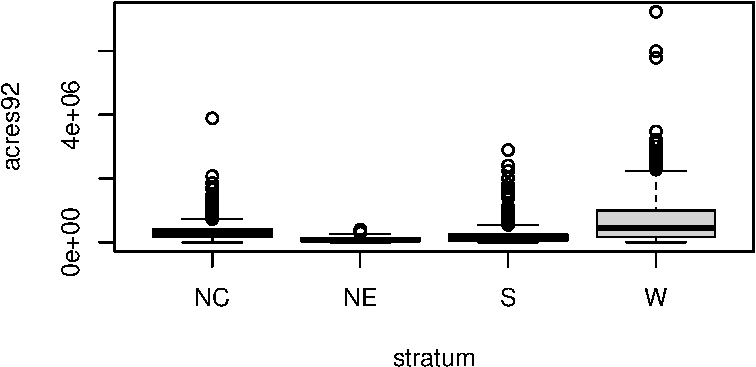
\includegraphics[keepaspectratio]{strata_files/figure-pdf/agpop-region-anova-1.pdf}}

\begin{verbatim}
Analysis of Variance Table

Response: agpop$acres92
                Df     Sum Sq    Mean Sq F value    Pr(>F)    
agpop$stratum    3 1.0073e+14 3.3578e+13  226.73 < 2.2e-16 ***
Residuals     3055 4.5243e+14 1.4810e+11                      
---
Signif. codes:  0 '***' 0.001 '**' 0.01 '*' 0.05 '.' 0.1 ' ' 1
\end{verbatim}

\begin{table}
\caption*{
{\fontsize{20}{25}\selectfont  Model Fit Summary\fontsize{12}{15}\selectfont }
} 
\fontsize{12.0pt}{14.0pt}\selectfont
\begin{tabular*}{0.7\linewidth}{@{\extracolsep{\fill}}rrrrr}
\toprule
\(R^2\) & Adj. \(R^2\) & \(\hat\sigma\) & F-statistic & p-value \\ 
\midrule\addlinespace[2.5pt]
0.1821 & 0.1813 & 384,831.7694 & 226.7299 & 0.0000 \\ 
\bottomrule
\end{tabular*}
\end{table}

\textbf{Output Note:} The R-squared is 0.182. The region variable only
explains about 18.2\% of the variance in acreage, which is helpful but
not extremely strong.

\subsubsection{Stratified Sampling with P2S allocation (Single
Run)}\label{stratified-sampling-with-p2s-allocation-single-run}

\begin{table}
\fontsize{12.0pt}{14.0pt}\selectfont
\begin{tabular*}{0.7\linewidth}{@{\extracolsep{\fill}}rrrr}
\toprule
\(\bar{y}\) & \(\mathrm{SE}(\bar{y})\) & 95\% CI Lower & 95\% CI Upper \\ 
\midrule\addlinespace[2.5pt]
295,589.9412 & 18,918.1011 & 258,510.4630 & 332,669.4194 \\ 
\bottomrule
\end{tabular*}
\end{table}

\textbf{Output Note:} This provides a single point estimate for
demonstration.

\subsubsection{Repeat stratified sampling with P2S allocation 2000
times}\label{repeat-stratified-sampling-with-p2s-allocation-2000-times}

\subsubsection{Repeat stratified sampling with optimal allocation 2000
times}\label{repeat-stratified-sampling-with-optimal-allocation-2000-times}

\begin{table}
\fontsize{12.0pt}{14.0pt}\selectfont
\begin{tabular*}{\linewidth}{@{\extracolsep{\fill}}l|rrr}
\toprule
 & Nh & Sh & nh\_opt \\ 
\midrule\addlinespace[2.5pt]
NC & 1052 & 271,187.98 & 87 \\ 
NE & 213 & 78,906.20 & 5 \\ 
S & 1376 & 244,131.98 & 102 \\ 
W & 418 & 836,613.56 & 106 \\ 
\bottomrule
\end{tabular*}
\end{table}

\textbf{Output Note:} This table compares the population sizes to the
optimal sample sizes. Notice that the West region (high variance) gets a
disproportionately larger sample under Neyman allocation.

\subsubsection{Repeat simple random sampling 2000
times}\label{repeat-simple-random-sampling-2000-times}

\subsubsection{Compare the efficiency of different
methods}\label{compare-the-efficiency-of-different-methods}

\pandocbounded{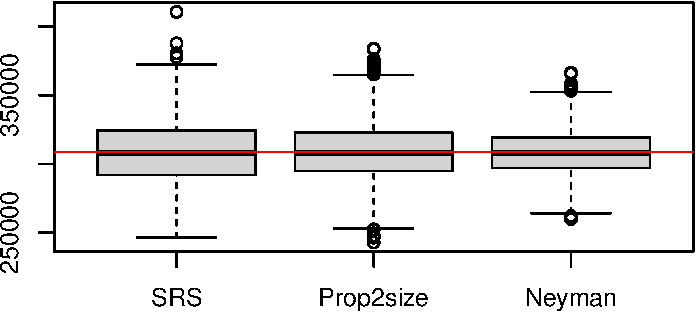
\includegraphics[keepaspectratio]{strata_files/figure-pdf/agpop-region-compare-plot-1.pdf}}

\textbf{Output Note:} The plot visually demonstrates that Neyman
allocation has the tightest spread around the true mean (the red line).

\begin{table}
\fontsize{12.0pt}{14.0pt}\selectfont
\begin{tabular*}{\linewidth}{@{\extracolsep{\fill}}l|rrrr}
\toprule
 & Mean & Variance & Relative Variance & Percentage of Variance Reduction \\ 
\midrule\addlinespace[2.5pt]
SRS & 308,818.2 & 547,160,924.7 & 1.000 & 0.00\% \\ 
Prop2size & 308,934.9 & 452,690,789.8 & 0.827 & 17.27\% \\ 
Neyman & 308,340.2 & 294,427,723.7 & 0.538 & 46.19\% \\ 
\bottomrule
\end{tabular*}
\end{table}

\textbf{Output Note:} The table summarizes the simulation. Proportional
allocation reduces variance by 17.3\%, while Neyman allocation reduces
it by 46.2\% compared to Simple Random Sampling.

\subsection{Using ``acres82'' to Define
Strata}\label{using-acres82-to-define-strata}

What if we stratify by a variable highly correlated with our target,
like the acreage from a decade prior (\texttt{acres82})?

\subsubsection{Read Population Data}\label{read-population-data-1}

\subsubsection{Define Stratum Variable with Quantiles of
``acres82''}\label{define-stratum-variable-with-quantiles-of-acres82}

We convert the continuous \texttt{acres82} variable into four distinct
categorical strata based on quantiles.

Let's check the explanatory power of this new stratification variable.

\pandocbounded{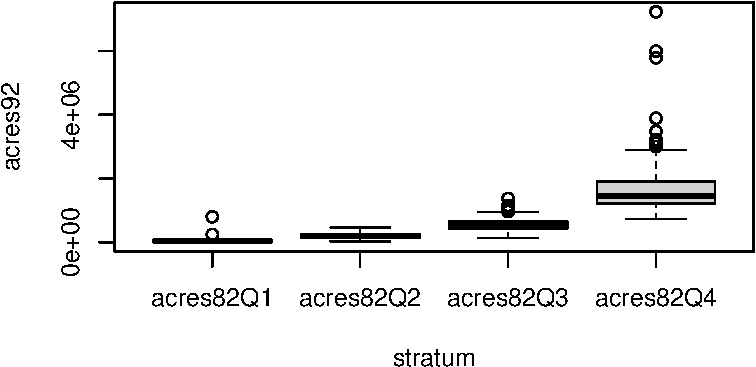
\includegraphics[keepaspectratio]{strata_files/figure-pdf/agpop-acres82-anova-1.pdf}}

\begin{table}
\caption*{
{\fontsize{20}{25}\selectfont  Model Fit Summary\fontsize{12}{15}\selectfont }
} 
\fontsize{12.0pt}{14.0pt}\selectfont
\begin{tabular*}{0.7\linewidth}{@{\extracolsep{\fill}}rrrrr}
\toprule
\(R^2\) & Adj. \(R^2\) & \(\hat\sigma\) & F-statistic & p-value \\ 
\midrule\addlinespace[2.5pt]
0.7393 & 0.7390 & 217,264.2290 & 2,887.8873 & 0.0000 \\ 
\bottomrule
\end{tabular*}
\end{table}

\textbf{Output Note:} The R-squared is 0.739. The past acreage explains
73.9\% of the variance in 1992 acreage, making this a vastly superior
stratification variable.

\subsubsection{Stratified sampling with P2S
allocation}\label{stratified-sampling-with-p2s-allocation}

\subsubsection{Repeat stratified sampling with optimal allocation 2000
times}\label{repeat-stratified-sampling-with-optimal-allocation-2000-times-1}

\subsubsection{Repeat simple random sampling 2000
times}\label{repeat-simple-random-sampling-2000-times-1}

\subsubsection{Compare the efficiency of different
methods}\label{compare-the-efficiency-of-different-methods-1}

\pandocbounded{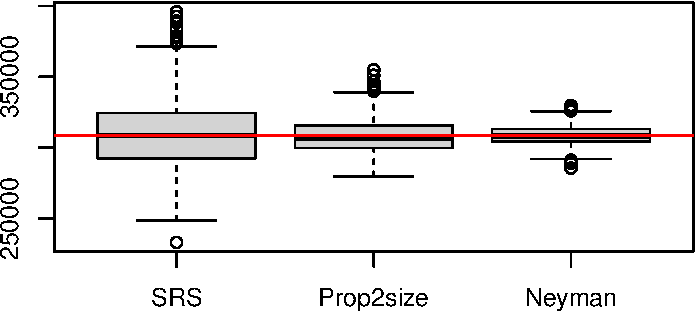
\includegraphics[keepaspectratio]{strata_files/figure-pdf/agpop-acres82-compare-plot-1.pdf}}

\textbf{Output Note:} The boxplot visually highlights a massive
reduction in variance compared to SRS, especially for the Neyman
allocation.

\begin{table}
\fontsize{12.0pt}{14.0pt}\selectfont
\begin{tabular*}{\linewidth}{@{\extracolsep{\fill}}l|rrrr}
\toprule
 & Mean & Variance & Relative Variance & Percentage of Variance Reduction \\ 
\midrule\addlinespace[2.5pt]
SRS & 309,511.5 & 549,602,264.4 & 1.000 & 0.00\% \\ 
Prop2size & 308,267.4 & 133,504,327.8 & 0.243 & 75.71\% \\ 
Neyman & 308,690.0 & 38,783,485.8 & 0.071 & 92.94\% \\ 
\bottomrule
\end{tabular*}
\end{table}

\textbf{Output Note:} The table shows dramatic results: Proportional
allocation reduces variance by 75.7\%, and Neyman allocation reduces it
by 92.9\%. Stratifying by a highly correlated variable is immensely
powerful.

\bookmarksetup{startatroot}

\chapter{Ratio, Regression, and Domain
Estimation}\label{ratio-regression-and-domain-estimation}

\begin{tcolorbox}[enhanced jigsaw, arc=.35mm, bottomrule=.15mm, bottomtitle=1mm, breakable, colback=white, colbacktitle=quarto-callout-note-color!10!white, colframe=quarto-callout-note-color-frame, coltitle=black, left=2mm, leftrule=.75mm, opacityback=0, opacitybacktitle=0.6, rightrule=.15mm, title=\textcolor{quarto-callout-note-color}{\faInfo}\hspace{0.5em}{Key formulae}, titlerule=0mm, toprule=.15mm, toptitle=1mm]

When auxiliary information (a variable \(x\)) is highly correlated with
our target variable of interest (\(y\)), we can use \textbf{Ratio} or
\textbf{Regression} estimation to improve precision without increasing
the sample size. We can also use auxiliary population structures to
adjust our estimates after the fact via \textbf{Post-stratification}, or
estimate means for specific sub-populations (\textbf{Domains}).

\subsubsection*{1. Ratio Estimation}\label{ratio-estimation}
\addcontentsline{toc}{subsubsection}{1. Ratio Estimation}

If the relationship between \(y\) and \(x\) passes through the origin,
we estimate the ratio \(B\) and use it to adjust the mean:

\begin{itemize}
\item
  \textbf{Ratio:} \(\hat{B} = \frac{\overline{y}}{\overline{x}}\)
\item
  \textbf{Mean Estimator:}
  \(\overline{y}_r = \hat{B} \overline{x}_{\text{U}}\) (where
  \(\overline{x}_{\text{U}}\) is the true population mean of \(x\))
\item
  \textbf{Estimated Variance:}
  \(\hat{V}(\overline{y}_r) = \left(\frac{\overline{x}_{\text{U}}}{\overline{x}}\right)^2 \left(1 - \frac{n}{N}\right) \frac{s_e^2}{n}\),
  where \(s_e^2\) is the sample variance of the residuals
  \(e_i = y_i - \hat{B}x_i\).
\end{itemize}

\subsubsection*{2. Regression Estimation}\label{regression-estimation}
\addcontentsline{toc}{subsubsection}{2. Regression Estimation}

If the relationship does not pass through the origin, a linear
regression is more appropriate:

\begin{itemize}
\tightlist
\item
  \textbf{Mean Estimator:}
  \(\overline{y}_{reg} = \hat{B}_0 + \hat{B}_1 \overline{x}_{\text{U}}\)
  (where \(\hat{B}_0\) and \(\hat{B}_1\) are OLS coefficients)
\item
  \textbf{Estimated Variance:}
  \(\hat{V}(\overline{y}_{reg}) = \left(1 - \frac{n}{N}\right) \frac{s_e^2}{n}\),
  where \(s_e^2\) is the Mean Square Error (Residuals) from the
  regression.
\end{itemize}

\subsubsection*{3. Domain Estimation}\label{domain-estimation}
\addcontentsline{toc}{subsubsection}{3. Domain Estimation}

To estimate the mean of a subgroup (domain \(d\)) when the domain sample
size \(n_d\) is a random variable:

\begin{itemize}
\tightlist
\item
  \textbf{Mean Estimator:}
  \(\overline{y}_d = \frac{1}{n_d} \sum_{i \in U_d} y_i\)
\item
  \textbf{Estimated Variance:}
  \(\hat{V}(\overline{y}_d) = \left(1 - \frac{n}{N}\right) \frac{s_d^2}{n_d}\),
  where \(n\) is the overall sample size, \(N\) is the population size,
  and \(s_d^2\) is the sample variance of \(y\) among the \(n_d\) units
  observed in domain \(d\).
\end{itemize}

\subsubsection*{4. Post-stratification}\label{post-stratification}
\addcontentsline{toc}{subsubsection}{4. Post-stratification}

If we know the true population sizes (\(N_h\)) of strata, but we used a
Simple Random Sample, we can post-stratify to reduce variance. We
substitute \(n_h\) with expected proportional sample sizes:

\begin{itemize}
\tightlist
\item
  \(n_h^{post-strat} = n \frac{N_h}{N}\)
\end{itemize}

\end{tcolorbox}

\section{Functions and packages for Analyzing
Data}\label{functions-and-packages-for-analyzing-data-1}

We begin by loading the necessary libraries, including \texttt{gt} for
formatting mathematical tables, and defining our custom functions for
Ratio, Regression, Domain, and Post-stratified estimation. We also
define a versatile \texttt{gt} helper to render our estimation outputs
cleanly.

\subsection{General functions for ratio and regression
estimation}\label{general-functions-for-ratio-and-regression-estimation}

The estimating functions used throughout this book (including
\texttt{reg\_est}, \texttt{ratio\_est}, \texttt{domain\_est},
\texttt{srs\_est}, and the \texttt{format\_est\_gt} table-formatting
helper used below) live in a single shared file,
\texttt{samplingestimate.r}, which we source below.

For post-stratification, we reuse the shared \texttt{str\_est()}
stratified estimator, but we plug in the expected sample sizes
\(n_h = n \times \frac{N_h}{N}\) instead of the actual observed random
\(n_h\).

\section{Ratio Estimation for cherry.csv
dataset}\label{ratio-estimation-for-cherry.csv-dataset}

We want to estimate the volume of wood in cherry trees using their
diameter as an auxiliary variable.

\subsection{Importing data}\label{importing-data}

First, let's load the data and verify that a strong linear relationship
passing near the origin exists between volume and diameter.

\begin{table}
\fontsize{12.0pt}{14.0pt}\selectfont
\begin{tabular*}{\linewidth}{@{\extracolsep{\fill}}rrr}
\toprule
diameter & height & volume \\ 
\midrule\addlinespace[2.5pt]
8.3 & 70 & 10.3 \\ 
8.6 & 65 & 10.3 \\ 
8.8 & 63 & 10.2 \\ 
10.5 & 72 & 16.4 \\ 
10.7 & 81 & 18.8 \\ 
10.8 & 83 & 19.7 \\ 
\bottomrule
\end{tabular*}
\end{table}

\pandocbounded{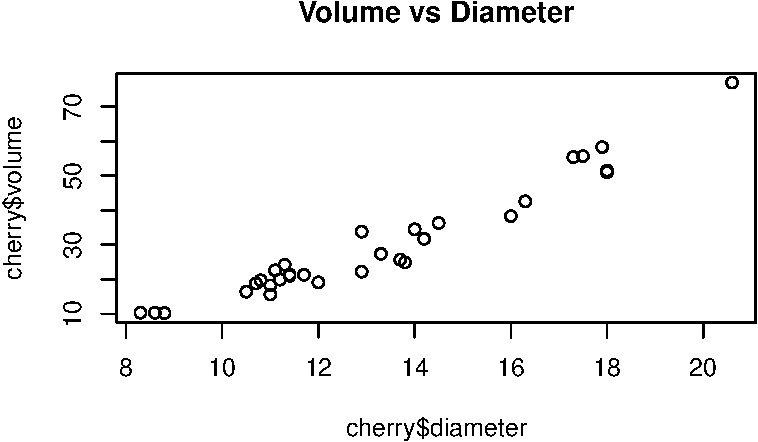
\includegraphics[keepaspectratio]{ratio_files/figure-pdf/cherry-load-plot-1.pdf}}

\begin{verbatim}
Analysis of Variance Table

Response: cherry$volume
                Df Sum Sq Mean Sq F value    Pr(>F)    
cherry$diameter  1  33622   33622  373.12 < 2.2e-16 ***
Residuals       30   2703      90                      
---
Signif. codes:  0 '***' 0.001 '**' 0.01 '*' 0.05 '.' 0.1 ' ' 1
\end{verbatim}

\textbf{Output Note:} The plot and the linear model output (which forces
a 0 intercept) confirm a very strong relationship, making this a prime
candidate for Ratio estimation.

\subsection{SRS estimate}\label{srs-estimate}

To establish a baseline, we first estimate the mean and total volume
using standard Simple Random Sampling (ignoring the auxiliary variable).

\begin{table}
\fontsize{12.0pt}{14.0pt}\selectfont
\begin{tabular*}{0.7\linewidth}{@{\extracolsep{\fill}}rrrr}
\toprule
\(\bar{y}\) & \(\mathrm{SE}(\bar{y})\) & 95\% CI Lower & 95\% CI Upper \\ 
\midrule\addlinespace[2.5pt]
30.1710 & 2.9369 & 24.1731 & 36.1688 \\ 
\bottomrule
\end{tabular*}
\end{table}

\begin{table}
\fontsize{12.0pt}{14.0pt}\selectfont
\begin{tabular*}{0.7\linewidth}{@{\extracolsep{\fill}}rrrr}
\toprule
\(\hat{t}\) & \(\mathrm{SE}(\hat{t})\) & 95\% CI Lower & 95\% CI Upper \\ 
\midrule\addlinespace[2.5pt]
89,517.2613 & 8,713.6652 & 71,721.5828 & 107,312.9398 \\ 
\bottomrule
\end{tabular*}
\end{table}

\textbf{Output Note:} Under SRS, the standard error for the mean volume
is 2.94.

\subsection{Ratio Estimation Using the
Function}\label{ratio-estimation-using-the-function}

We calculate the ratio \(\hat{B} = \overline{y}/\overline{x}\); the
function's \texttt{\$table} shows the row-level working values \(x_i\),
\(y_i\), fitted \(\hat{y}_i = \hat{B}x_i\), residuals
\(e_i = y_i - \hat{y}_i\), and \(e_i^2\) (with a Sum row and a footnote
giving \(\hat B\) and \(s_e^2\)), so we no longer need to build this
table by hand.

\begin{table}
\caption*{
{\fontsize{20}{25}\selectfont  Ratio Estimation: Working Table\fontsize{12}{15}\selectfont } \\ 
{\fontsize{14}{17}\selectfont  \(n = 31\)\fontsize{12}{15}\selectfont }
} 
\fontsize{12.0pt}{14.0pt}\selectfont
\begin{tabular*}{\linewidth}{@{\extracolsep{\fill}}>{\raggedright\arraybackslash}p{\dimexpr 30.00pt -2\tabcolsep-1.5\arrayrulewidth}>{\raggedleft\arraybackslash}p{\dimexpr 75.00pt -2\tabcolsep-1.5\arrayrulewidth}>{\raggedleft\arraybackslash}p{\dimexpr 75.00pt -2\tabcolsep-1.5\arrayrulewidth}>{\raggedleft\arraybackslash}p{\dimexpr 75.00pt -2\tabcolsep-1.5\arrayrulewidth}>{\raggedleft\arraybackslash}p{\dimexpr 75.00pt -2\tabcolsep-1.5\arrayrulewidth}>{\raggedleft\arraybackslash}p{\dimexpr 75.00pt -2\tabcolsep-1.5\arrayrulewidth}}
\toprule
\(i\) & \(y_i\) & \(x_i\) & \(\hat y_i\)\textsuperscript{\textit{1}} & \(e_i\) & \(e_i^2\) \\ 
\midrule\addlinespace[2.5pt]
1 & 10.300 & 8.300 & 18.902 & -8.602 & 73.992 \\ 
2 & 10.300 & 8.600 & 19.585 & -9.285 & 86.212 \\ 
3 & 10.200 & 8.800 & 20.041 & -9.841 & 96.836 \\ 
4 & 16.400 & 10.500 & 23.912 & -7.512 & 56.430 \\ 
5 & 18.800 & 10.700 & 24.367 & -5.567 & 30.996 \\ 
6 & 19.700 & 10.800 & 24.595 & -4.895 & 23.963 \\ 
... & ... & ... & ... & ... & ... \\ 
{\bfseries Sum} & {\bfseries 935.300} & {\bfseries 410.700} & {\bfseries 935.300} & {\bfseries 3.553 $\times$ 10\textsuperscript{-14}} & {\bfseries 2,821.586} \\ 
\bottomrule
\end{tabular*}
\begin{minipage}{\linewidth}
\vspace{.05em}
\textsuperscript{\textit{1}}\(\hat B = \sum_i y_i / \sum_i x_i = 2.2773\), \(\hat y_i = \hat B\, x_i\), \(s_e^2 = 94.0529\).\\
\textbf{Point estimate:} \(\hat B = \dfrac{\sum_i y_i}{\sum_i x_i} = \dfrac{935.300}{410.700} = 2.277\)\\
\textbf{Standard error:} \(\mathrm{SE}(\hat B) = \dfrac{1}{\bar x}\sqrt{\left(1-\dfrac{n}{N}\right)\dfrac{s_e^2}{n}} = \dfrac{1}{13.248}\sqrt{\left(1-\dfrac{31}{2967}\right)\dfrac{94.053}{31}} = 0.131\)\\
\end{minipage}
\end{table}

\pandocbounded{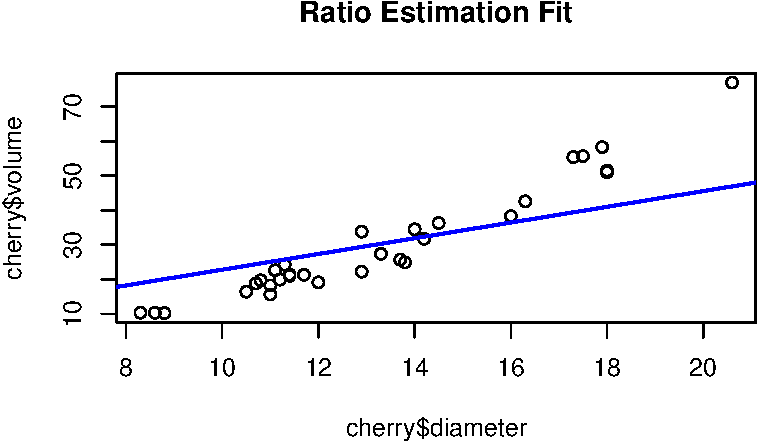
\includegraphics[keepaspectratio]{ratio_files/figure-pdf/cherry-ratio-est-1.pdf}}

\textbf{Output Note:} The blue line represents our estimated ratio
\(\hat{B} \approx 2.28\). The working table above shows the individual
residuals used to estimate \(s_e^2\).

\begin{table}
\fontsize{12.0pt}{14.0pt}\selectfont
\begin{tabular*}{0.7\linewidth}{@{\extracolsep{\fill}}rrrr}
\toprule
\(\hat{B}\) & \(\mathrm{SE}(\hat{B})\) & 95\% CI Lower & 95\% CI Upper \\ 
\midrule\addlinespace[2.5pt]
2.2773 & 0.1308 & 2.0102 & 2.5444 \\ 
\bottomrule
\end{tabular*}
\end{table}

\textbf{Output Note:} The ratio \(\hat{B}\) is estimated at 2.277 with a
standard error of 0.1308.

\subsubsection{Estimating the mean volume of
wood}\label{estimating-the-mean-volume-of-wood}

If we know the true total of the population diameters is 41,835, we can
derive the population mean diameter \(\overline{x}_{\text{U}}\) and pass
it as \texttt{xbarU} with \texttt{estimate\ =\ "mean"}.

\begin{table}
\caption*{
{\fontsize{20}{25}\selectfont  Ratio Estimation: Working Table\fontsize{12}{15}\selectfont } \\ 
{\fontsize{14}{17}\selectfont  \(n = 31\)\fontsize{12}{15}\selectfont }
} 
\fontsize{12.0pt}{14.0pt}\selectfont
\begin{tabular*}{\linewidth}{@{\extracolsep{\fill}}>{\raggedright\arraybackslash}p{\dimexpr 30.00pt -2\tabcolsep-1.5\arrayrulewidth}>{\raggedleft\arraybackslash}p{\dimexpr 75.00pt -2\tabcolsep-1.5\arrayrulewidth}>{\raggedleft\arraybackslash}p{\dimexpr 75.00pt -2\tabcolsep-1.5\arrayrulewidth}>{\raggedleft\arraybackslash}p{\dimexpr 75.00pt -2\tabcolsep-1.5\arrayrulewidth}>{\raggedleft\arraybackslash}p{\dimexpr 75.00pt -2\tabcolsep-1.5\arrayrulewidth}>{\raggedleft\arraybackslash}p{\dimexpr 75.00pt -2\tabcolsep-1.5\arrayrulewidth}}
\toprule
\(i\) & \(y_i\) & \(x_i\) & \(\hat y_i\)\textsuperscript{\textit{1}} & \(e_i\) & \(e_i^2\) \\ 
\midrule\addlinespace[2.5pt]
1 & 10.300 & 8.300 & 18.902 & -8.602 & 73.992 \\ 
2 & 10.300 & 8.600 & 19.585 & -9.285 & 86.212 \\ 
3 & 10.200 & 8.800 & 20.041 & -9.841 & 96.836 \\ 
4 & 16.400 & 10.500 & 23.912 & -7.512 & 56.430 \\ 
5 & 18.800 & 10.700 & 24.367 & -5.567 & 30.996 \\ 
6 & 19.700 & 10.800 & 24.595 & -4.895 & 23.963 \\ 
... & ... & ... & ... & ... & ... \\ 
{\bfseries Sum} & {\bfseries 935.300} & {\bfseries 410.700} & {\bfseries 935.300} & {\bfseries 3.553 $\times$ 10\textsuperscript{-14}} & {\bfseries 2,821.586} \\ 
\bottomrule
\end{tabular*}
\begin{minipage}{\linewidth}
\vspace{.05em}
\textsuperscript{\textit{1}}\(\hat B = \sum_i y_i / \sum_i x_i = 2.2773\), \(\hat y_i = \hat B\, x_i\), \(s_e^2 = 94.0529\).\\
\textbf{Point estimate:} \(\bar y_r = \hat B\,\bar x_U = 2.277 \times 14.100 = 32.111\)\\
\textbf{Standard error:} \(\mathrm{SE}(\bar y_r) = \mathrm{SE}(\hat B)\,\bar x_U = 0.131 \times 14.100 = 1.844\)\\
\end{minipage}
\end{table}

\begin{table}
\fontsize{12.0pt}{14.0pt}\selectfont
\begin{tabular*}{0.7\linewidth}{@{\extracolsep{\fill}}rrrr}
\toprule
\(\bar{y}_{r}\) & \(\mathrm{SE}(\bar{y}_{r})\) & 95\% CI Lower & 95\% CI Upper \\ 
\midrule\addlinespace[2.5pt]
32.1106 & 1.8441 & 28.3445 & 35.8768 \\ 
\bottomrule
\end{tabular*}
\end{table}

\subsubsection{Estimating the total volume of
wood}\label{estimating-the-total-volume-of-wood}

Using \texttt{estimate\ =\ "total"} with the known population total
diameter gives the estimated population total volume directly.

\begin{table}
\caption*{
{\fontsize{20}{25}\selectfont  Ratio Estimation: Working Table\fontsize{12}{15}\selectfont } \\ 
{\fontsize{14}{17}\selectfont  \(n = 31\)\fontsize{12}{15}\selectfont }
} 
\fontsize{12.0pt}{14.0pt}\selectfont
\begin{tabular*}{\linewidth}{@{\extracolsep{\fill}}>{\raggedright\arraybackslash}p{\dimexpr 30.00pt -2\tabcolsep-1.5\arrayrulewidth}>{\raggedleft\arraybackslash}p{\dimexpr 75.00pt -2\tabcolsep-1.5\arrayrulewidth}>{\raggedleft\arraybackslash}p{\dimexpr 75.00pt -2\tabcolsep-1.5\arrayrulewidth}>{\raggedleft\arraybackslash}p{\dimexpr 75.00pt -2\tabcolsep-1.5\arrayrulewidth}>{\raggedleft\arraybackslash}p{\dimexpr 75.00pt -2\tabcolsep-1.5\arrayrulewidth}>{\raggedleft\arraybackslash}p{\dimexpr 75.00pt -2\tabcolsep-1.5\arrayrulewidth}}
\toprule
\(i\) & \(y_i\) & \(x_i\) & \(\hat y_i\)\textsuperscript{\textit{1}} & \(e_i\) & \(e_i^2\) \\ 
\midrule\addlinespace[2.5pt]
1 & 10.300 & 8.300 & 18.902 & -8.602 & 73.992 \\ 
2 & 10.300 & 8.600 & 19.585 & -9.285 & 86.212 \\ 
3 & 10.200 & 8.800 & 20.041 & -9.841 & 96.836 \\ 
4 & 16.400 & 10.500 & 23.912 & -7.512 & 56.430 \\ 
5 & 18.800 & 10.700 & 24.367 & -5.567 & 30.996 \\ 
6 & 19.700 & 10.800 & 24.595 & -4.895 & 23.963 \\ 
... & ... & ... & ... & ... & ... \\ 
{\bfseries Sum} & {\bfseries 935.300} & {\bfseries 410.700} & {\bfseries 935.300} & {\bfseries 3.553 $\times$ 10\textsuperscript{-14}} & {\bfseries 2,821.586} \\ 
\bottomrule
\end{tabular*}
\begin{minipage}{\linewidth}
\vspace{.05em}
\textsuperscript{\textit{1}}\(\hat B = \sum_i y_i / \sum_i x_i = 2.2773\), \(\hat y_i = \hat B\, x_i\), \(s_e^2 = 94.0529\).\\
\textbf{Point estimate:} \(\hat t = \hat B\,\bar x_U\,N = 2.277 \times 14.100 \times 2,967 = 95,272.159\)\\
\textbf{Standard error:} \(\mathrm{SE}(\hat t) = \mathrm{SE}(\hat B)\,\bar x_U\,N = 0.131 \times 14.100 \times 2,967 = 5,471.434\)\\
\end{minipage}
\end{table}

\begin{table}
\fontsize{12.0pt}{14.0pt}\selectfont
\begin{tabular*}{0.7\linewidth}{@{\extracolsep{\fill}}rrrr}
\toprule
\(\hat{t}\) & \(\mathrm{SE}(\hat{t})\) & 95\% CI Lower & 95\% CI Upper \\ 
\midrule\addlinespace[2.5pt]
95,272.1585 & 5,471.4344 & 84,097.9988 & 106,446.3182 \\ 
\bottomrule
\end{tabular*}
\end{table}

\subsubsection{Percentage of Variance
Reduction}\label{percentage-of-variance-reduction}

How much did ratio estimation help compared to ignoring the auxiliary
variable?

\begin{verbatim}
[1] 0.6057237
\end{verbatim}

\textbf{Output Note:} Using the diameter as an auxiliary variable
reduced the variance of our estimate by 60.6\% compared to simple random
sampling.

\section{Simulation study with
agpop.csv}\label{simulation-study-with-agpop.csv}

Let's test this practically by drawing 2000 random samples and seeing
how SRS and Ratio estimators behave under repeated sampling.

\subsection{Information of population
data}\label{information-of-population-data}

\pandocbounded{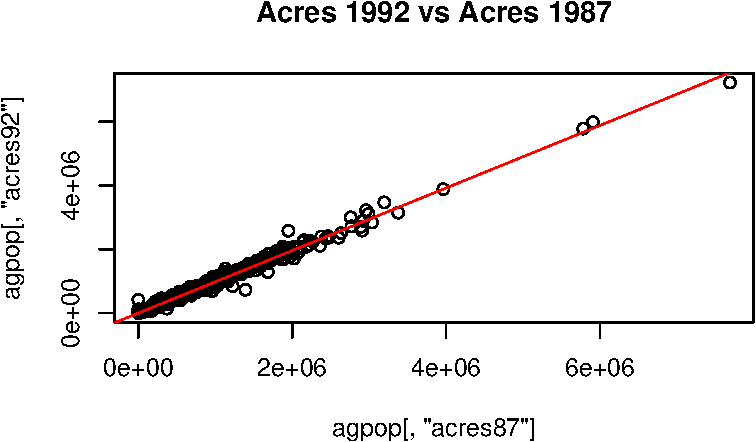
\includegraphics[keepaspectratio]{ratio_files/figure-pdf/agpop-load-1.pdf}}

\begin{table}
\caption*{
{\fontsize{20}{25}\selectfont  Coefficient Estimates\fontsize{12}{15}\selectfont }
} 
\fontsize{12.0pt}{14.0pt}\selectfont
\begin{tabular*}{0.7\linewidth}{@{\extracolsep{\fill}}l|rrrr}
\toprule
 & Estimate & S.E. & t value & p value \\ 
\midrule\addlinespace[2.5pt]
(Intercept) & -2,121.4881 & 864.7615 & -2.4533 & 0.0142 \\ 
agpop\$acres87 & 0.9878 & 0.0016 & 607.3876 & 0.0000 \\ 
\bottomrule
\end{tabular*}
\end{table}

\begin{table}
\caption*{
{\fontsize{20}{25}\selectfont  Model Fit Summary\fontsize{12}{15}\selectfont }
} 
\fontsize{12.0pt}{14.0pt}\selectfont
\begin{tabular*}{0.7\linewidth}{@{\extracolsep{\fill}}rrrrr}
\toprule
\(R^2\) & Adj. \(R^2\) & \(\hat\sigma\) & F-statistic & p-value \\ 
\midrule\addlinespace[2.5pt]
0.9918 & 0.9918 & 38,562.8752 & 368,919.6409 & 0.0000 \\ 
\bottomrule
\end{tabular*}
\end{table}

\begin{verbatim}
[1] 0.9917355
\end{verbatim}

\textbf{Output Note:} Past acreage (1987) strongly predicts current
acreage (1992). The theoretically expected variance reduction is roughly
99.2\%.

\subsection{Simulation Studies}\label{simulation-studies}

\pandocbounded{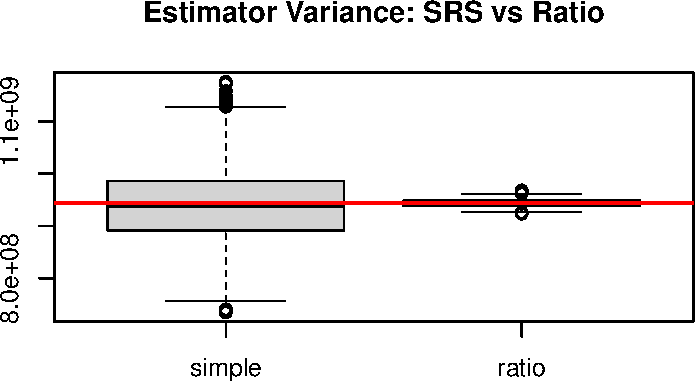
\includegraphics[keepaspectratio]{ratio_files/figure-pdf/agpop-simulation-1.pdf}}

We now calculate the actual variance across our 2000 simulations.

\begin{table}
\fontsize{12.0pt}{14.0pt}\selectfont
\begin{tabular*}{\linewidth}{@{\extracolsep{\fill}}l|rrr}
\toprule
 & Variance & Relative Variance & Variance Reduction \\ 
\midrule\addlinespace[2.5pt]
simple & 5,001,990,416,619,630 & 1.0000 & 0.00\% \\ 
ratio & 42,824,673,244,644 & 0.0086 & 99.14\% \\ 
\bottomrule
\end{tabular*}
\end{table}

\textbf{Output Note:} The boxplot dramatically illustrates the precision
gain. The variance of the ratio estimator is only 0.9\% of the SRS
variance, confirming our theoretical expectations.

\section{Estimating Domain Means and Post-stratification with agsrs.csv
example}\label{estimating-domain-means-and-post-stratification-with-agsrs.csv-example}

\subsection{Estimating Domain Means}\label{estimating-domain-means}

When estimating the mean for a specific subgroup (like a region), the
sample size in that subgroup (\(n_d\)) is a random variable, which
increases our uncertainty.

\begin{table}
\fontsize{12.0pt}{14.0pt}\selectfont
\begin{tabular*}{0.7\linewidth}{@{\extracolsep{\fill}}l|rrrr}
\toprule
 & \(\bar{y}_{d}\) & \(\mathrm{SE}(\bar{y}_{d})\) & 95\% CI Lower & 95\% CI Upper \\ 
\midrule\addlinespace[2.5pt]
NC & 323,416.4359 & 30,008.3469 & 263,662.1833 & 383,170.6885 \\ 
NE & 106,549.0000 & 28,957.5582 & 45,453.8926 & 167,644.1074 \\ 
S & 246,185.8375 & 23,503.6178 & 199,766.2813 & 292,605.3937 \\ 
W & 518,977.6364 & 70,298.6900 & 377,206.8165 & 660,748.4562 \\ 
\bottomrule
\end{tabular*}
\end{table}

If we incorrectly used the standard SRS formula (pretending \(n_d\) was
fixed), our standard errors would be artificially low:

\begin{table}
\fontsize{12.0pt}{14.0pt}\selectfont
\begin{tabular*}{0.7\linewidth}{@{\extracolsep{\fill}}l|rrrr}
\toprule
 & \(\bar{y}\) & \(\mathrm{SE}(\bar{y})\) & 95\% CI Lower & 95\% CI Upper \\ 
\midrule\addlinespace[2.5pt]
NC & 323,416.4359 & 30,395.8898 & 262,890.4867 & 383,942.3851 \\ 
NE & 106,549.0000 & 29,207.5056 & 44,926.5496 & 168,171.4504 \\ 
S & 246,185.8375 & 23,264.0052 & 200,239.5154 & 292,132.1596 \\ 
W & 518,977.6364 & 70,033.3811 & 377,741.8630 & 660,213.4097 \\ 
\bottomrule
\end{tabular*}
\end{table}

\textbf{Output Note:} Comparing the two tables, you can see the correct
\texttt{domain\_mean} Standard Errors are larger, appropriately
penalizing us for the uncertainty in how many counties from each region
randomly fell into our sample.

\subsection{Post-stratification
Analysis}\label{post-stratification-analysis}

If we know the true regional population sizes (\(N_h\)), we can
post-stratify our SRS data.

\textbf{Create \(n_h^{\text{post-strat}} = n \times \frac{N_h}{N}\)},
instead of using the randomly observed \(n_h\).

\begin{table}
\fontsize{12.0pt}{14.0pt}\selectfont
\begin{tabular*}{\linewidth}{@{\extracolsep{\fill}}l|rrrrrrr}
\toprule
 & \(\bar{y}_h\) & \(s_h\) & \(n_h^{\text{obs}}\) & \(\pi^{\text{obs}}_h\) & \(N_h\) & \(\pi^{\text{pop}}_h\) & \(n_h^{\text{post}}\) \\ 
\midrule\addlinespace[2.5pt]
NC & 323,416.436 & 278,970.037 & 78 & 0.260 & 1054 & 0.342 & 102.729 \\ 
NE & 106,549.000 & 129,320.203 & 18 & 0.060 & 220 & 0.071 & 21.442 \\ 
S & 246,185.837 & 312,941.310 & 160 & 0.533 & 1382 & 0.449 & 134.698 \\ 
W & 518,977.636 & 490,842.046 & 44 & 0.147 & 422 & 0.137 & 41.131 \\ 
\bottomrule
\end{tabular*}
\end{table}

\textbf{Output Note:} The table above shows the difference between the
sample proportion (\(\pi^{obs}_h\)) and the true population proportion
(\(\pi^{pop}_h\)). Post-stratification forces the weights to reflect the
true population structure.

\begin{table}
\caption*{
{\fontsize{20}{25}\selectfont  Stratified Mean Estimation: Working Table\fontsize{12}{15}\selectfont }
} 
\fontsize{12.0pt}{14.0pt}\selectfont
\begin{tabular*}{\linewidth}{@{\extracolsep{\fill}}>{\raggedright\arraybackslash}p{\dimexpr 82.50pt -2\tabcolsep-1.5\arrayrulewidth}>{\raggedleft\arraybackslash}p{\dimexpr 45.00pt -2\tabcolsep-1.5\arrayrulewidth}>{\raggedleft\arraybackslash}p{\dimexpr 45.00pt -2\tabcolsep-1.5\arrayrulewidth}>{\raggedleft\arraybackslash}p{\dimexpr 82.50pt -2\tabcolsep-1.5\arrayrulewidth}>{\raggedleft\arraybackslash}p{\dimexpr 82.50pt -2\tabcolsep-1.5\arrayrulewidth}>{\raggedleft\arraybackslash}p{\dimexpr 82.50pt -2\tabcolsep-1.5\arrayrulewidth}>{\raggedleft\arraybackslash}p{\dimexpr 82.50pt -2\tabcolsep-1.5\arrayrulewidth}>{\raggedleft\arraybackslash}p{\dimexpr 82.50pt -2\tabcolsep-1.5\arrayrulewidth}}
\toprule
Stratum & \(N_h\) & \(n_h\) & \(\pi_h\)\textsuperscript{\textit{1}} & \(\bar y_h\) & \(s_h^2\) & \(\pi_h\bar y_h\) & \(v_h\)\textsuperscript{\textit{2}} \\ 
\midrule\addlinespace[2.5pt]
NC & 1,054 & 103 & 0.34 & 3.23 $\times$ 10\textsuperscript{5} & 7.78 $\times$ 10\textsuperscript{10} & 1.11 $\times$ 10\textsuperscript{5} & 8.02 $\times$ 10\textsuperscript{7} \\ 
NE & 220 & 21 & 0.07 & 1.07 $\times$ 10\textsuperscript{5} & 1.67 $\times$ 10\textsuperscript{10} & 7.62 $\times$ 10\textsuperscript{3} & 3.60 $\times$ 10\textsuperscript{6} \\ 
S & 1,382 & 135 & 0.45 & 2.46 $\times$ 10\textsuperscript{5} & 9.79 $\times$ 10\textsuperscript{10} & 1.11 $\times$ 10\textsuperscript{5} & 1.32 $\times$ 10\textsuperscript{8} \\ 
W & 422 & 41 & 0.14 & 5.19 $\times$ 10\textsuperscript{5} & 2.41 $\times$ 10\textsuperscript{11} & 7.12 $\times$ 10\textsuperscript{4} & 9.94 $\times$ 10\textsuperscript{7} \\ 
{\bfseries Total} & {\bfseries 3,078} & {\bfseries 300} & {\bfseries 1.00} & {\bfseries } & {\bfseries } & {\bfseries 3.00 $\times$ 10\textsuperscript{5}} & {\bfseries 3.15 $\times$ 10\textsuperscript{8}} \\ 
\bottomrule
\end{tabular*}
\begin{minipage}{\linewidth}
\vspace{.05em}
\textsuperscript{\textit{1}}\(\pi_h = N_h/N\) is the stratum weight.\\
\textsuperscript{\textit{2}}\(v_h = (1-n_h/N_h)\,\pi_h^2\, s_h^2/n_h\) is stratum \(h\)'s contribution to \(V(\bar y_{str}) = \sum_h v_h\).\\
\textbf{Point estimate:} \(\bar y_{str} = \sum_h \pi_h\bar y_h = 3.001 \times 10^{5}\)\\
\textbf{Standard error:} \(\mathrm{SE}(\bar y_{str}) = \sqrt{\sum_h v_h} = \sqrt{3.154 \times 10^{8}} = 17,760.257\)\\
\end{minipage}
\end{table}

\begin{table}
\fontsize{12.0pt}{14.0pt}\selectfont
\begin{tabular*}{0.7\linewidth}{@{\extracolsep{\fill}}rrrr}
\toprule
\(\bar{y}\) & \(\mathrm{SE}(\bar{y})\) & 95\% CI Lower & 95\% CI Upper \\ 
\midrule\addlinespace[2.5pt]
300,051.6873 & 17,760.2566 & 265,241.5844 & 334,861.7901 \\ 
\bottomrule
\end{tabular*}
\end{table}

\begin{table}
\fontsize{12.0pt}{14.0pt}\selectfont
\begin{tabular*}{0.7\linewidth}{@{\extracolsep{\fill}}rrrr}
\toprule
\(\bar{y}\) & \(\mathrm{SE}(\bar{y})\) & 95\% CI Lower & 95\% CI Upper \\ 
\midrule\addlinespace[2.5pt]
297,897.0467 & 18,901.4092 & 260,700.4027 & 335,093.6907 \\ 
\bottomrule
\end{tabular*}
\end{table}

\begin{verbatim}
[1] 308582.4
\end{verbatim}

\textbf{Output Note:} The post-stratified estimate gives a Standard
Error of \ensuremath{1.77603\times 10^{4}}, which is more precise than
the unadjusted SRS standard error of \ensuremath{1.89014\times 10^{4}}.

\section{Estimating Domain Means and Post-stratification with teacher
example}\label{estimating-domain-means-and-post-stratification-with-teacher-example}

\subsection{Importing Data and Calculating Contingency
Table}\label{importing-data-and-calculating-contingency-table}

\begin{verbatim}
      teacher
gender   0   1
     1 156  84
     2 120  40
\end{verbatim}

\begin{verbatim}
      teacher
gender   0   1 Sum
     1 156  84 240
     2 120  40 160
\end{verbatim}

\begin{verbatim}
      teacher
gender    0    1
     1 0.65 0.35
     2 0.75 0.25
\end{verbatim}

\subsection{Domain Summary}\label{domain-summary}

\begin{table}
\fontsize{12.0pt}{14.0pt}\selectfont
\begin{tabular*}{\linewidth}{@{\extracolsep{\fill}}l|rrrr}
\toprule
 & \(\bar{y}_h\) & \(s_h\) & \(n^{\text{obs}}_h\) & \(\pi^{\text{obs}}_h\) \\ 
\midrule\addlinespace[2.5pt]
1 & 0.350 & 0.478 & 240.000 & 0.600 \\ 
2 & 0.250 & 0.434 & 160.000 & 0.400 \\ 
\bottomrule
\end{tabular*}
\end{table}

\subsection{Estimating Domain Means}\label{estimating-domain-means-1}

\begin{table}
\fontsize{12.0pt}{14.0pt}\selectfont
\begin{tabular*}{0.7\linewidth}{@{\extracolsep{\fill}}l|rrrr}
\toprule
 & \(\bar{y}_{d}\) & \(\mathrm{SE}(\bar{y}_{d})\) & 95\% CI Lower & 95\% CI Upper \\ 
\midrule\addlinespace[2.5pt]
female & 0.3500 & 0.0293 & 0.2923 & 0.4077 \\ 
male & 0.2500 & 0.0326 & 0.1857 & 0.3143 \\ 
\bottomrule
\end{tabular*}
\end{table}

\subsection{Post-stratification
Analysis}\label{post-stratification-analysis-1}

\begin{verbatim}
[1] 0.75 0.25
\end{verbatim}

\subsubsection*{\texorpdfstring{Create
\(n_h^{\text{post-strat}} = n \times \frac{N_h}{N}\)}{Create n\_h\^{}\{\textbackslash text\{post-strat\}\} = n \textbackslash times \textbackslash frac\{N\_h\}\{N\}}}\label{create-n_htextpost-strat-n-times-fracn_hn}
\addcontentsline{toc}{subsubsection}{Create
\(n_h^{\text{post-strat}} = n \times \frac{N_h}{N}\)}

\begin{table}
\fontsize{12.0pt}{14.0pt}\selectfont
\begin{tabular*}{\linewidth}{@{\extracolsep{\fill}}l|rrrrrrr}
\toprule
 & \(\hat{p}_h\) & \(s_h\) & \(n_h\) & \(\pi^{\text{obs}}_h\) & \(N_h\) & \(\pi^{\text{pop}}_h\) & \(n_h^{\text{post-strat}}\) \\ 
\midrule\addlinespace[2.5pt]
1 & 0.350 & 0.478 & 240 & 0.600 & 3000 & 0.750 & 300.000 \\ 
2 & 0.250 & 0.434 & 160 & 0.400 & 1000 & 0.250 & 100.000 \\ 
\bottomrule
\end{tabular*}
\end{table}

Calculate the post-stratification estimation of the mean:

\begin{table}
\caption*{
{\fontsize{20}{25}\selectfont  Stratified Mean Estimation: Working Table\fontsize{12}{15}\selectfont }
} 
\fontsize{12.0pt}{14.0pt}\selectfont
\begin{tabular*}{\linewidth}{@{\extracolsep{\fill}}>{\raggedright\arraybackslash}p{\dimexpr 82.50pt -2\tabcolsep-1.5\arrayrulewidth}>{\raggedleft\arraybackslash}p{\dimexpr 45.00pt -2\tabcolsep-1.5\arrayrulewidth}>{\raggedleft\arraybackslash}p{\dimexpr 45.00pt -2\tabcolsep-1.5\arrayrulewidth}>{\raggedleft\arraybackslash}p{\dimexpr 82.50pt -2\tabcolsep-1.5\arrayrulewidth}>{\raggedleft\arraybackslash}p{\dimexpr 82.50pt -2\tabcolsep-1.5\arrayrulewidth}>{\raggedleft\arraybackslash}p{\dimexpr 82.50pt -2\tabcolsep-1.5\arrayrulewidth}>{\raggedleft\arraybackslash}p{\dimexpr 82.50pt -2\tabcolsep-1.5\arrayrulewidth}>{\raggedleft\arraybackslash}p{\dimexpr 82.50pt -2\tabcolsep-1.5\arrayrulewidth}}
\toprule
Stratum & \(N_h\) & \(n_h\) & \(\pi_h\)\textsuperscript{\textit{1}} & \(\bar y_h\) & \(s_h^2\) & \(\pi_h\bar y_h\) & \(v_h\)\textsuperscript{\textit{2}} \\ 
\midrule\addlinespace[2.5pt]
1 & 3,000 & 300 & 0.75 & 0.35 & 0.23 & 0.26 & 3.86 $\times$ 10\textsuperscript{-4} \\ 
2 & 1,000 & 100 & 0.25 & 0.25 & 0.19 & 0.06 & 1.06 $\times$ 10\textsuperscript{-4} \\ 
{\bfseries Total} & {\bfseries 4,000} & {\bfseries 400} & {\bfseries 1.00} & {\bfseries } & {\bfseries } & {\bfseries 0.32} & {\bfseries 4.92 $\times$ 10\textsuperscript{-4}} \\ 
\bottomrule
\end{tabular*}
\begin{minipage}{\linewidth}
\vspace{.05em}
\textsuperscript{\textit{1}}\(\pi_h = N_h/N\) is the stratum weight.\\
\textsuperscript{\textit{2}}\(v_h = (1-n_h/N_h)\,\pi_h^2\, s_h^2/n_h\) is stratum \(h\)'s contribution to \(V(\bar y_{str}) = \sum_h v_h\).\\
\textbf{Point estimate:} \(\bar y_{str} = \sum_h \pi_h\bar y_h = 0.325\)\\
\textbf{Standard error:} \(\mathrm{SE}(\bar y_{str}) = \sqrt{\sum_h v_h} = \sqrt{4.916 \times 10^{-4}} = 0.022\)\\
\end{minipage}
\end{table}

\begin{table}
\fontsize{12.0pt}{14.0pt}\selectfont
\begin{tabular*}{0.7\linewidth}{@{\extracolsep{\fill}}rrrr}
\toprule
\(\bar{y}\) & \(\mathrm{SE}(\bar{y})\) & 95\% CI Lower & 95\% CI Upper \\ 
\midrule\addlinespace[2.5pt]
0.3250 & 0.0222 & 0.2815 & 0.3685 \\ 
\bottomrule
\end{tabular*}
\end{table}

This post-stratification estimate explicitly corrects for the sampling
imbalance using the true strata sizes:

\begin{verbatim}
    1 
0.325 
\end{verbatim}

\subsection{Comparing to the Analysis with
SRS}\label{comparing-to-the-analysis-with-srs}

If we didn't post-stratify, the simple mean is heavily weighted toward
males because they were over-sampled by chance (40\% in sample vs 25\%
in population).

\begin{verbatim}
NULL
\end{verbatim}

\begin{table}
\fontsize{12.0pt}{14.0pt}\selectfont
\begin{tabular*}{0.7\linewidth}{@{\extracolsep{\fill}}rrrr}
\toprule
\(\bar{y}\) & \(\mathrm{SE}(\bar{y})\) & 95\% CI Lower & 95\% CI Upper \\ 
\midrule\addlinespace[2.5pt]
0.3100 & 0.0220 & 0.2668 & 0.3532 \\ 
\bottomrule
\end{tabular*}
\end{table}

This equals the naive sample proportion:

\begin{verbatim}
[1] 0.31
\end{verbatim}

\section{Regression Estimation for the cherry.csv
dataset}\label{regression-estimation-for-the-cherry.csv-dataset}

When the relationship between \(y\) and \(x\) doesn't pass exactly
through the origin, we use Regression Estimation.

\subsection{Importing data}\label{importing-data-1}

\subsection{Regression Estimation Using the
Function}\label{regression-estimation-using-the-function}

\subsubsection{Fitting a linear regression
model}\label{fitting-a-linear-regression-model}

\begin{table}
\caption*{
{\fontsize{20}{25}\selectfont  Coefficient Estimates\fontsize{12}{15}\selectfont }
} 
\fontsize{12.0pt}{14.0pt}\selectfont
\begin{tabular*}{0.7\linewidth}{@{\extracolsep{\fill}}l|rrrr}
\toprule
 & Estimate & S.E. & t value & p value \\ 
\midrule\addlinespace[2.5pt]
(Intercept) & -36.9435 & 3.3651 & -10.9783 & 0.0000 \\ 
xdata & 5.0659 & 0.2474 & 20.4783 & 0.0000 \\ 
\bottomrule
\end{tabular*}
\end{table}

\begin{table}
\caption*{
{\fontsize{20}{25}\selectfont  Model Fit Summary\fontsize{12}{15}\selectfont }
} 
\fontsize{12.0pt}{14.0pt}\selectfont
\begin{tabular*}{0.7\linewidth}{@{\extracolsep{\fill}}rrrrr}
\toprule
\(R^2\) & Adj. \(R^2\) & \(\hat\sigma\) & F-statistic & p-value \\ 
\midrule\addlinespace[2.5pt]
0.9353 & 0.9331 & 4.2520 & 419.3603 & 0.0000 \\ 
\bottomrule
\end{tabular*}
\end{table}

\pandocbounded{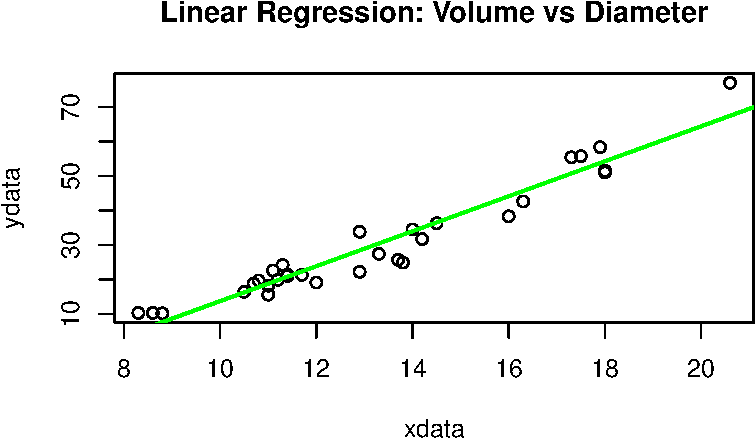
\includegraphics[keepaspectratio]{ratio_files/figure-pdf/cherry-reg-fit-1.pdf}}

The function's \texttt{\$table} shows the row-level working values
\(x_i\), \(y_i\), fitted \(\hat{y}_i = \hat{B}_0 + \hat{B}_1 x_i\),
residuals \(e_i = y_i - \hat{y}_i\), and \(e_i^2\) (with a Sum row and a
footnote giving \(\hat B_0\), \(\hat B_1\), and \(s_e^2\)):

\begin{table}
\caption*{
{\fontsize{20}{25}\selectfont  Regression Estimation: Working Table\fontsize{12}{15}\selectfont } \\ 
{\fontsize{14}{17}\selectfont  \(n = 31\)\fontsize{12}{15}\selectfont }
} 
\fontsize{12.0pt}{14.0pt}\selectfont
\begin{tabular*}{\linewidth}{@{\extracolsep{\fill}}>{\raggedright\arraybackslash}p{\dimexpr 30.00pt -2\tabcolsep-1.5\arrayrulewidth}>{\raggedleft\arraybackslash}p{\dimexpr 75.00pt -2\tabcolsep-1.5\arrayrulewidth}>{\raggedleft\arraybackslash}p{\dimexpr 75.00pt -2\tabcolsep-1.5\arrayrulewidth}>{\raggedleft\arraybackslash}p{\dimexpr 75.00pt -2\tabcolsep-1.5\arrayrulewidth}>{\raggedleft\arraybackslash}p{\dimexpr 75.00pt -2\tabcolsep-1.5\arrayrulewidth}>{\raggedleft\arraybackslash}p{\dimexpr 75.00pt -2\tabcolsep-1.5\arrayrulewidth}}
\toprule
\(i\) & \(y_i\) & \(x_i\) & \(\hat y_i\)\textsuperscript{\textit{1}} & \(e_i\) & \(e_i^2\) \\ 
\midrule\addlinespace[2.5pt]
1 & 10.300 & 8.300 & 5.103 & 5.197 & 27.007 \\ 
2 & 10.300 & 8.600 & 6.623 & 3.677 & 13.521 \\ 
3 & 10.200 & 8.800 & 7.636 & 2.564 & 6.574 \\ 
4 & 16.400 & 10.500 & 16.248 & 1.520 $\times$ 10\textsuperscript{-1} & 0.023 \\ 
5 & 18.800 & 10.700 & 17.261 & 1.539 & 2.368 \\ 
6 & 19.700 & 10.800 & 17.768 & 1.932 & 3.733 \\ 
... & ... & ... & ... & ... & ... \\ 
{\bfseries Sum} & {\bfseries 935.300} & {\bfseries 410.700} & {\bfseries 935.300} & {\bfseries -3.553 $\times$ 10\textsuperscript{-15}} & {\bfseries 524.303} \\ 
\bottomrule
\end{tabular*}
\begin{minipage}{\linewidth}
\vspace{.05em}
\textsuperscript{\textit{1}}\(\hat B_0 = -36.9435\), \(\hat B_1 = 5.0659\), \(\hat y_i = \hat B_0 + \hat B_1 x_i\), \(s_e^2 = 18.0794\).\\
\textbf{Point estimate:} \(\hat B_1 = \dfrac{\sum_i(x_i-\bar x)(y_i-\bar y)}{\sum_i(x_i-\bar x)^2} = \dfrac{1,496.644}{295.437} = 5.066\)\\
\textbf{Standard error:} \(\mathrm{SE}(\hat B_1) = \sqrt{\dfrac{s_e^2}{\sum_i(x_i-\bar x)^2}} = \sqrt{\dfrac{18.079}{295.437}} = 0.247\)\\
\end{minipage}
\end{table}

\subsubsection{Estimate the mean}\label{estimate-the-mean}

We compute the regression estimate \(\overline{y}_{reg}\) by passing
\texttt{xbarU} with \texttt{estimate\ =\ "mean"}.

\begin{table}
\caption*{
{\fontsize{20}{25}\selectfont  Regression Estimation: Working Table\fontsize{12}{15}\selectfont } \\ 
{\fontsize{14}{17}\selectfont  \(n = 31\)\fontsize{12}{15}\selectfont }
} 
\fontsize{12.0pt}{14.0pt}\selectfont
\begin{tabular*}{\linewidth}{@{\extracolsep{\fill}}>{\raggedright\arraybackslash}p{\dimexpr 30.00pt -2\tabcolsep-1.5\arrayrulewidth}>{\raggedleft\arraybackslash}p{\dimexpr 75.00pt -2\tabcolsep-1.5\arrayrulewidth}>{\raggedleft\arraybackslash}p{\dimexpr 75.00pt -2\tabcolsep-1.5\arrayrulewidth}>{\raggedleft\arraybackslash}p{\dimexpr 75.00pt -2\tabcolsep-1.5\arrayrulewidth}>{\raggedleft\arraybackslash}p{\dimexpr 75.00pt -2\tabcolsep-1.5\arrayrulewidth}>{\raggedleft\arraybackslash}p{\dimexpr 75.00pt -2\tabcolsep-1.5\arrayrulewidth}}
\toprule
\(i\) & \(y_i\) & \(x_i\) & \(\hat y_i\)\textsuperscript{\textit{1}} & \(e_i\) & \(e_i^2\) \\ 
\midrule\addlinespace[2.5pt]
1 & 10.300 & 8.300 & 5.103 & 5.197 & 27.007 \\ 
2 & 10.300 & 8.600 & 6.623 & 3.677 & 13.521 \\ 
3 & 10.200 & 8.800 & 7.636 & 2.564 & 6.574 \\ 
4 & 16.400 & 10.500 & 16.248 & 1.520 $\times$ 10\textsuperscript{-1} & 0.023 \\ 
5 & 18.800 & 10.700 & 17.261 & 1.539 & 2.368 \\ 
6 & 19.700 & 10.800 & 17.768 & 1.932 & 3.733 \\ 
... & ... & ... & ... & ... & ... \\ 
{\bfseries Sum} & {\bfseries 935.300} & {\bfseries 410.700} & {\bfseries 935.300} & {\bfseries -3.553 $\times$ 10\textsuperscript{-15}} & {\bfseries 524.303} \\ 
\bottomrule
\end{tabular*}
\begin{minipage}{\linewidth}
\vspace{.05em}
\textsuperscript{\textit{1}}\(\hat B_0 = -36.9435\), \(\hat B_1 = 5.0659\), \(\hat y_i = \hat B_0 + \hat B_1 x_i\), \(s_e^2 = 18.0794\).\\
\textbf{Point estimate:} \(\bar y_{reg} = \hat B_0+\hat B_1\bar x_U = -36.943 + 5.066 \times 14.100 = 34.486\)\\
\textbf{Standard error:} \(\mathrm{SE}(\bar y_{reg}) = \sqrt{\left(1-\dfrac{n}{N}\right)\dfrac{s_e^2}{n}} = \sqrt{\left(1-\dfrac{31}{2967}\right)\dfrac{18.079}{31}} = 0.760\)\\
\end{minipage}
\end{table}

\begin{table}
\fontsize{12.0pt}{14.0pt}\selectfont
\begin{tabular*}{0.7\linewidth}{@{\extracolsep{\fill}}rrrr}
\toprule
\(\bar{y}_{reg}\) & \(\mathrm{SE}(\bar{y}_{reg})\) & 95\% CI Lower & 95\% CI Upper \\ 
\midrule\addlinespace[2.5pt]
34.4856 & 0.7597 & 32.9319 & 36.0393 \\ 
\bottomrule
\end{tabular*}
\end{table}

\textbf{Output Note:} The Regression estimate for the mean volume is
34.486 with a standard error of 0.7597.

\subsubsection{Estimate the total}\label{estimate-the-total}

\begin{table}
\fontsize{12.0pt}{14.0pt}\selectfont
\begin{tabular*}{0.7\linewidth}{@{\extracolsep{\fill}}rrrr}
\toprule
\(\hat{t}_{reg}\) & \(\mathrm{SE}(\hat{t}_{reg})\) & 95\% CI Lower & 95\% CI Upper \\ 
\midrule\addlinespace[2.5pt]
102,318.8602 & 2,253.9690 & 97,708.9761 & 106,928.7444 \\ 
\bottomrule
\end{tabular*}
\end{table}

\subsubsection{Percentage of Variance
Reduction}\label{percentage-of-variance-reduction-1}

\begin{verbatim}
[1] 0.9330895
\end{verbatim}

\textbf{Output Note:} The variance reduction for the regression
estimator is 93.3\%, which is similar to the ratio estimator since the
true intercept is very close to zero.

\section{Regression estimation for photo counts of dead
trees}\label{regression-estimation-for-photo-counts-of-dead-trees}

To estimate the number of dead trees in an area, we divide the area into
100 square plots and count dead trees on photographs. We select an SRS
of 25 plots for exact field counts. We know the true mean photo count is
11.3.

\begin{table}
\caption*{
{\fontsize{20}{25}\selectfont  Coefficient Estimates\fontsize{12}{15}\selectfont }
} 
\fontsize{12.0pt}{14.0pt}\selectfont
\begin{tabular*}{0.7\linewidth}{@{\extracolsep{\fill}}l|rrrr}
\toprule
 & Estimate & S.E. & t value & p value \\ 
\midrule\addlinespace[2.5pt]
(Intercept) & 5.0593 & 1.7635 & 2.8689 & 0.0087 \\ 
photocounts & 0.6133 & 0.1601 & 3.8316 & 0.0009 \\ 
\bottomrule
\end{tabular*}
\end{table}

\begin{table}
\caption*{
{\fontsize{20}{25}\selectfont  Model Fit Summary\fontsize{12}{15}\selectfont }
} 
\fontsize{12.0pt}{14.0pt}\selectfont
\begin{tabular*}{0.7\linewidth}{@{\extracolsep{\fill}}rrrrr}
\toprule
\(R^2\) & Adj. \(R^2\) & \(\hat\sigma\) & F-statistic & p-value \\ 
\midrule\addlinespace[2.5pt]
0.3896 & 0.3631 & 2.4062 & 14.6815 & 0.0009 \\ 
\bottomrule
\end{tabular*}
\end{table}

\pandocbounded{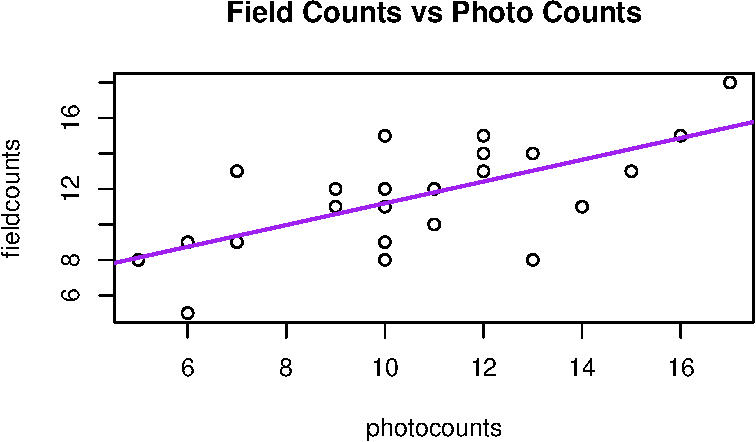
\includegraphics[keepaspectratio]{ratio_files/figure-pdf/deadtrees-data-1.pdf}}

Let's compare the three different estimation methods to see which
provides the lowest Standard Error for the population mean.

\begin{table}
\caption*{
{\fontsize{20}{25}\selectfont  Regression Estimation: Working Table\fontsize{12}{15}\selectfont } \\ 
{\fontsize{14}{17}\selectfont  \(n = 25\)\fontsize{12}{15}\selectfont }
} 
\fontsize{12.0pt}{14.0pt}\selectfont
\begin{tabular*}{\linewidth}{@{\extracolsep{\fill}}>{\raggedright\arraybackslash}p{\dimexpr 30.00pt -2\tabcolsep-1.5\arrayrulewidth}>{\raggedleft\arraybackslash}p{\dimexpr 75.00pt -2\tabcolsep-1.5\arrayrulewidth}>{\raggedleft\arraybackslash}p{\dimexpr 75.00pt -2\tabcolsep-1.5\arrayrulewidth}>{\raggedleft\arraybackslash}p{\dimexpr 75.00pt -2\tabcolsep-1.5\arrayrulewidth}>{\raggedleft\arraybackslash}p{\dimexpr 75.00pt -2\tabcolsep-1.5\arrayrulewidth}>{\raggedleft\arraybackslash}p{\dimexpr 75.00pt -2\tabcolsep-1.5\arrayrulewidth}}
\toprule
\(i\) & \(y_i\) & \(x_i\) & \(\hat y_i\)\textsuperscript{\textit{1}} & \(e_i\) & \(e_i^2\) \\ 
\midrule\addlinespace[2.5pt]
1 & 15.000 & 10.000 & 11.192 & 3.808 & 14.501 \\ 
2 & 14.000 & 12.000 & 12.419 & 1.581 & 2.501 \\ 
3 & 9.000 & 7.000 & 9.352 & -3.522 $\times$ 10\textsuperscript{-1} & 0.124 \\ 
4 & 14.000 & 13.000 & 13.032 & 9.681 $\times$ 10\textsuperscript{-1} & 0.937 \\ 
5 & 8.000 & 13.000 & 13.032 & -5.032 & 25.320 \\ 
6 & 5.000 & 6.000 & 8.739 & -3.739 & 13.980 \\ 
... & ... & ... & ... & ... & ... \\ 
{\bfseries Sum} & {\bfseries 289.000} & {\bfseries 265.000} & {\bfseries 289.000} & {\bfseries -2.665 $\times$ 10\textsuperscript{-15}} & {\bfseries 133.160} \\ 
\bottomrule
\end{tabular*}
\begin{minipage}{\linewidth}
\vspace{.05em}
\textsuperscript{\textit{1}}\(\hat B_0 = 5.0593\), \(\hat B_1 = 0.6133\), \(\hat y_i = \hat B_0 + \hat B_1 x_i\), \(s_e^2 = 5.7896\).\\
\textbf{Point estimate:} \(\bar y_{reg} = \hat B_0+\hat B_1\bar x_U = 5.059 + 0.613 \times 11.300 = 11.989\)\\
\textbf{Standard error:} \(\mathrm{SE}(\bar y_{reg}) = \sqrt{\left(1-\dfrac{n}{N}\right)\dfrac{s_e^2}{n}} = \sqrt{\left(1-\dfrac{25}{100}\right)\dfrac{5.790}{25}} = 0.417\)\\
\end{minipage}
\end{table}

\begin{table}
\fontsize{12.0pt}{14.0pt}\selectfont
\begin{tabular*}{0.7\linewidth}{@{\extracolsep{\fill}}rrrr}
\toprule
\(\bar{y}_{reg}\) & \(\mathrm{SE}(\bar{y}_{reg})\) & 95\% CI Lower & 95\% CI Upper \\ 
\midrule\addlinespace[2.5pt]
11.9893 & 0.4168 & 11.1272 & 12.8514 \\ 
\bottomrule
\end{tabular*}
\end{table}

\begin{table}
\fontsize{12.0pt}{14.0pt}\selectfont
\begin{tabular*}{0.7\linewidth}{@{\extracolsep{\fill}}rrrr}
\toprule
\(\hat{t}_{reg}\) & \(\mathrm{SE}(\hat{t}_{reg})\) & 95\% CI Lower & 95\% CI Upper \\ 
\midrule\addlinespace[2.5pt]
1,198.9292 & 41.6758 & 1,112.7163 & 1,285.1422 \\ 
\bottomrule
\end{tabular*}
\end{table}

\begin{table}
\fontsize{12.0pt}{14.0pt}\selectfont
\begin{tabular*}{0.7\linewidth}{@{\extracolsep{\fill}}rrrr}
\toprule
\(\bar{y}\) & \(\mathrm{SE}(\bar{y})\) & 95\% CI Lower & 95\% CI Upper \\ 
\midrule\addlinespace[2.5pt]
11.5600 & 0.5222 & 10.4822 & 12.6378 \\ 
\bottomrule
\end{tabular*}
\end{table}

\begin{table}
\caption*{
{\fontsize{20}{25}\selectfont  Ratio Estimation: Working Table\fontsize{12}{15}\selectfont } \\ 
{\fontsize{14}{17}\selectfont  \(n = 25\)\fontsize{12}{15}\selectfont }
} 
\fontsize{12.0pt}{14.0pt}\selectfont
\begin{tabular*}{\linewidth}{@{\extracolsep{\fill}}>{\raggedright\arraybackslash}p{\dimexpr 30.00pt -2\tabcolsep-1.5\arrayrulewidth}>{\raggedleft\arraybackslash}p{\dimexpr 75.00pt -2\tabcolsep-1.5\arrayrulewidth}>{\raggedleft\arraybackslash}p{\dimexpr 75.00pt -2\tabcolsep-1.5\arrayrulewidth}>{\raggedleft\arraybackslash}p{\dimexpr 75.00pt -2\tabcolsep-1.5\arrayrulewidth}>{\raggedleft\arraybackslash}p{\dimexpr 75.00pt -2\tabcolsep-1.5\arrayrulewidth}>{\raggedleft\arraybackslash}p{\dimexpr 75.00pt -2\tabcolsep-1.5\arrayrulewidth}}
\toprule
\(i\) & \(y_i\) & \(x_i\) & \(\hat y_i\)\textsuperscript{\textit{1}} & \(e_i\) & \(e_i^2\) \\ 
\midrule\addlinespace[2.5pt]
1 & 15.000 & 10.000 & 10.906 & 4.094 & 16.764 \\ 
2 & 14.000 & 12.000 & 13.087 & 9.132 $\times$ 10\textsuperscript{-1} & 0.834 \\ 
3 & 9.000 & 7.000 & 7.634 & 1.366 & 1.866 \\ 
4 & 14.000 & 13.000 & 14.177 & -1.774 $\times$ 10\textsuperscript{-1} & 0.031 \\ 
5 & 8.000 & 13.000 & 14.177 & -6.177 & 38.160 \\ 
6 & 5.000 & 6.000 & 6.543 & -1.543 & 2.382 \\ 
... & ... & ... & ... & ... & ... \\ 
{\bfseries Sum} & {\bfseries 289.000} & {\bfseries 265.000} & {\bfseries 289.000} & {\bfseries 5.329 $\times$ 10\textsuperscript{-15}} & {\bfseries 184.645} \\ 
\bottomrule
\end{tabular*}
\begin{minipage}{\linewidth}
\vspace{.05em}
\textsuperscript{\textit{1}}\(\hat B = \sum_i y_i / \sum_i x_i = 1.0906\), \(\hat y_i = \hat B\, x_i\), \(s_e^2 = 7.6935\).\\
\textbf{Point estimate:} \(\bar y_r = \hat B\,\bar x_U = 1.091 \times 11.300 = 12.323\)\\
\textbf{Standard error:} \(\mathrm{SE}(\bar y_r) = \mathrm{SE}(\hat B)\,\bar x_U = 0.045 \times 11.300 = 0.512\)\\
\end{minipage}
\end{table}

\begin{table}
\fontsize{12.0pt}{14.0pt}\selectfont
\begin{tabular*}{0.7\linewidth}{@{\extracolsep{\fill}}rrrr}
\toprule
\(\bar{y}_{r}\) & \(\mathrm{SE}(\bar{y}_{r})\) & 95\% CI Lower & 95\% CI Upper \\ 
\midrule\addlinespace[2.5pt]
12.3234 & 0.5121 & 11.2664 & 13.3804 \\ 
\bottomrule
\end{tabular*}
\end{table}

\subsubsection*{Output Note:}\label{output-note}
\addcontentsline{toc}{subsubsection}{Output Note:}

\begin{itemize}
\item
  \textbf{SRS Mean:} SE = 0.522
\item
  \textbf{Ratio Mean:} SE = 0.512
\item
  \textbf{Regression Mean:} SE = 0.417
\end{itemize}

Because the intercept of the true line is non-zero, the
\textbf{Regression estimator} provides the most precise estimate in this
scenario.

\bookmarksetup{startatroot}

\chapter{Cluster Sampling}\label{cluster-sampling}

\section{Key Formulas for Cluster
Sampling}\label{key-formulas-for-cluster-sampling}

Cluster sampling divides the population into \(N\) clusters, out of
which a simple random sample of \(n\) clusters is selected. This design
is highly practical when a sampling frame of individual elements is
unavailable, or when individuals are geographically grouped.

\subsubsection*{1. One-Stage Cluster
Sampling}\label{one-stage-cluster-sampling}
\addcontentsline{toc}{subsubsection}{1. One-Stage Cluster Sampling}

In a one-stage design, every element \(M_i\) within the sampled cluster
\(i\) is surveyed.

\begin{itemize}
\item
  \textbf{Total in Cluster \(i\):} \(t_i = \sum_{j=1}^{M_i} y_{ij}\)
\item
  \textbf{Ratio Estimator of the Population Mean:} The ratio estimator
  leverages cluster sizes to estimate the overall element mean: \[
  \overline{y}_r = \frac{\sum_{i=1}^n t_i}{\sum_{i=1}^n M_i}.
  \]
\item
  \textbf{Estimated Variance of the Mean:} \[
  \hat{V}(\overline{y}_r) = \left(1 - \frac{n}{N}\right) \frac{1}{n\overline{M}^2} \frac{\sum_{i=1}^n (t_i - \overline{y}_r M_i)^2}{n-1}.
  \]
\end{itemize}

\subsubsection*{2. Two-Stage Cluster
Sampling}\label{two-stage-cluster-sampling}
\addcontentsline{toc}{subsubsection}{2. Two-Stage Cluster Sampling}

In a two-stage design, we first sample \(n\) clusters, then take a
subsample of \(m_i\) elements from the \(M_i\) elements within each
selected cluster. Because we don't observe the true cluster total
\(t_i\), we estimate it:

\begin{itemize}
\tightlist
\item
  \textbf{Estimated Total in Cluster \(i\):}
  \(\hat{t}_i = M_i \overline{y}_i\), where
  \(\overline{y}_i = \frac{1}{m_i} \sum_{j=1}^{m_i} y_{ij}\)
\item
  \textbf{Ratio Estimator of the Population Mean:} \[
  \overline{y}_r = \frac{\sum_{i=1}^n \hat{t}_i}{\sum_{i=1}^n M_i}
  \]
\end{itemize}

\begin{center}\rule{0.5\linewidth}{0.5pt}\end{center}

\section{Functions and packages for Analyzing
Data}\label{functions-and-packages-for-analyzing-data-2}

The estimating functions used throughout this book (including
\texttt{cluster\_ratio}, used below for one-stage and two-stage cluster
samples) live in a single shared file, \texttt{samplingestimate.r},
which we source below.

\section{Estimating for One-stage cluster sampling: analysis of
algebra.csv}\label{estimating-for-one-stage-cluster-sampling-analysis-of-algebra.csv}

Consider a population of 187 high school algebra classes in a city. An
investigator takes an SRS of 12 of those classes (the clusters). Because
this is a one-stage sample, every student in the 12 sampled classes
takes the test to evaluate their function knowledge.

We read the raw data and display it using \texttt{gt}'s interactive
pagination feature to keep the document clean.

\begin{table}
\caption*{
{\fontsize{20}{25}\selectfont  Raw Data: Algebra Classes\fontsize{12}{15}\selectfont }
} 
\fontsize{12.0pt}{14.0pt}\selectfont
\begin{tabular*}{\linewidth}{@{\extracolsep{\fill}}rrr}
\toprule
class & M<sub>i</sub> & score \\ 
\midrule\addlinespace[2.5pt]
23 & 20 & 57 \\ 
23 & 20 & 90 \\ 
23 & 20 & 56 \\ 
23 & 20 & 57 \\ 
23 & 20 & 46 \\ 
23 & 20 & 55 \\ 
23 & 20 & 62 \\ 
23 & 20 & 66 \\ 
23 & 20 & 78 \\ 
23 & 20 & 76 \\ 
23 & 20 & 57 \\ 
23 & 20 & 84 \\ 
23 & 20 & 27 \\ 
23 & 20 & 70 \\ 
23 & 20 & 49 \\ 
23 & 20 & 82 \\ 
23 & 20 & 52 \\ 
23 & 20 & 82 \\ 
23 & 20 & 59 \\ 
23 & 20 & 25 \\ 
37 & 26 & 57 \\ 
37 & 26 & 34 \\ 
37 & 26 & 68 \\ 
37 & 26 & 99 \\ 
37 & 26 & 24 \\ 
37 & 26 & 83 \\ 
37 & 26 & 40 \\ 
37 & 26 & 98 \\ 
37 & 26 & 90 \\ 
37 & 26 & 50 \\ 
37 & 26 & 60 \\ 
37 & 26 & 64 \\ 
37 & 26 & 58 \\ 
37 & 26 & 100 \\ 
37 & 26 & 68 \\ 
37 & 26 & 52 \\ 
37 & 26 & 77 \\ 
37 & 26 & 69 \\ 
37 & 26 & 64 \\ 
37 & 26 & 64 \\ 
37 & 26 & 73 \\ 
37 & 26 & 46 \\ 
37 & 26 & 44 \\ 
37 & 26 & 95 \\ 
37 & 26 & 28 \\ 
37 & 26 & 65 \\ 
38 & 24 & 41 \\ 
38 & 24 & 66 \\ 
38 & 24 & 79 \\ 
38 & 24 & 24 \\ 
38 & 24 & 77 \\ 
38 & 24 & 60 \\ 
38 & 24 & 37 \\ 
38 & 24 & 26 \\ 
38 & 24 & 74 \\ 
38 & 24 & 58 \\ 
38 & 24 & 65 \\ 
38 & 24 & 76 \\ 
38 & 24 & 92 \\ 
38 & 24 & 59 \\ 
38 & 24 & 51 \\ 
38 & 24 & 87 \\ 
38 & 24 & 45 \\ 
38 & 24 & 40 \\ 
38 & 24 & 51 \\ 
38 & 24 & 100 \\ 
38 & 24 & 46 \\ 
38 & 24 & 68 \\ 
38 & 24 & 40 \\ 
38 & 24 & 40 \\ 
39 & 34 & 54 \\ 
39 & 34 & 84 \\ 
39 & 34 & 51 \\ 
39 & 34 & 75 \\ 
39 & 34 & 34 \\ 
39 & 34 & 53 \\ 
39 & 34 & 46 \\ 
39 & 34 & 53 \\ 
39 & 34 & 82 \\ 
39 & 34 & 58 \\ 
39 & 34 & 63 \\ 
39 & 34 & 64 \\ 
39 & 34 & 49 \\ 
39 & 34 & 34 \\ 
39 & 34 & 54 \\ 
39 & 34 & 62 \\ 
39 & 34 & 78 \\ 
39 & 34 & 55 \\ 
39 & 34 & 54 \\ 
39 & 34 & 89 \\ 
39 & 34 & 46 \\ 
39 & 34 & 67 \\ 
39 & 34 & 49 \\ 
39 & 34 & 67 \\ 
39 & 34 & 32 \\ 
39 & 34 & 50 \\ 
39 & 34 & 55 \\ 
39 & 34 & 78 \\ 
39 & 34 & 51 \\ 
39 & 34 & 65 \\ 
39 & 34 & 52 \\ 
39 & 34 & 44 \\ 
39 & 34 & 72 \\ 
39 & 34 & 52 \\ 
41 & 26 & 82 \\ 
41 & 26 & 65 \\ 
41 & 26 & 55 \\ 
41 & 26 & 65 \\ 
41 & 26 & 57 \\ 
41 & 26 & 65 \\ 
41 & 26 & 50 \\ 
41 & 26 & 19 \\ 
41 & 26 & 60 \\ 
41 & 26 & 69 \\ 
41 & 26 & 40 \\ 
41 & 26 & 37 \\ 
41 & 26 & 49 \\ 
41 & 26 & 48 \\ 
41 & 26 & 65 \\ 
41 & 26 & 60 \\ 
41 & 26 & 76 \\ 
41 & 26 & 87 \\ 
41 & 26 & 57 \\ 
41 & 26 & 57 \\ 
41 & 26 & 62 \\ 
41 & 26 & 51 \\ 
41 & 26 & 55 \\ 
41 & 26 & 55 \\ 
41 & 26 & 62 \\ 
41 & 26 & 60 \\ 
44 & 28 & 59 \\ 
44 & 28 & 65 \\ 
44 & 28 & 60 \\ 
44 & 28 & 78 \\ 
44 & 28 & 64 \\ 
44 & 28 & 52 \\ 
44 & 28 & 59 \\ 
44 & 28 & 51 \\ 
44 & 28 & 67 \\ 
44 & 28 & 79 \\ 
44 & 28 & 75 \\ 
44 & 28 & 67 \\ 
44 & 28 & 62 \\ 
44 & 28 & 69 \\ 
44 & 28 & 63 \\ 
44 & 28 & 27 \\ 
44 & 28 & 70 \\ 
44 & 28 & 57 \\ 
44 & 28 & 86 \\ 
44 & 28 & 100 \\ 
44 & 28 & 41 \\ 
44 & 28 & 74 \\ 
44 & 28 & 66 \\ 
44 & 28 & 54 \\ 
44 & 28 & 75 \\ 
44 & 28 & 76 \\ 
44 & 28 & 62 \\ 
44 & 28 & 58 \\ 
46 & 19 & 34 \\ 
46 & 19 & 42 \\ 
46 & 19 & 49 \\ 
46 & 19 & 49 \\ 
46 & 19 & 71 \\ 
46 & 19 & 49 \\ 
46 & 19 & 88 \\ 
46 & 19 & 46 \\ 
46 & 19 & 82 \\ 
46 & 19 & 57 \\ 
46 & 19 & 34 \\ 
46 & 19 & 64 \\ 
46 & 19 & 54 \\ 
46 & 19 & 47 \\ 
46 & 19 & 69 \\ 
46 & 19 & 63 \\ 
46 & 19 & 72 \\ 
46 & 19 & 35 \\ 
46 & 19 & 43 \\ 
51 & 32 & 58 \\ 
51 & 32 & 22 \\ 
51 & 32 & 82 \\ 
51 & 32 & 99 \\ 
51 & 32 & 88 \\ 
51 & 32 & 52 \\ 
51 & 32 & 61 \\ 
51 & 32 & 44 \\ 
51 & 32 & 98 \\ 
51 & 32 & 70 \\ 
51 & 32 & 59 \\ 
51 & 32 & 92 \\ 
51 & 32 & 72 \\ 
51 & 32 & 49 \\ 
51 & 32 & 76 \\ 
51 & 32 & 77 \\ 
51 & 32 & 79 \\ 
51 & 32 & 84 \\ 
51 & 32 & 65 \\ 
51 & 32 & 88 \\ 
51 & 32 & 55 \\ 
51 & 32 & 100 \\ 
51 & 32 & 65 \\ 
51 & 32 & 84 \\ 
51 & 32 & 87 \\ 
51 & 32 & 71 \\ 
51 & 32 & 47 \\ 
51 & 32 & 70 \\ 
51 & 32 & 66 \\ 
51 & 32 & 69 \\ 
51 & 32 & 91 \\ 
51 & 32 & 88 \\ 
58 & 17 & 61 \\ 
58 & 17 & 44 \\ 
58 & 17 & 100 \\ 
58 & 17 & 28 \\ 
58 & 17 & 28 \\ 
58 & 17 & 63 \\ 
58 & 17 & 100 \\ 
58 & 17 & 51 \\ 
58 & 17 & 34 \\ 
58 & 17 & 49 \\ 
58 & 17 & 100 \\ 
58 & 17 & 43 \\ 
58 & 17 & 48 \\ 
58 & 17 & 52 \\ 
58 & 17 & 70 \\ 
58 & 17 & 69 \\ 
58 & 17 & 49 \\ 
62 & 21 & 31 \\ 
62 & 21 & 99 \\ 
62 & 21 & 43 \\ 
62 & 21 & 57 \\ 
62 & 21 & 69 \\ 
62 & 21 & 73 \\ 
62 & 21 & 43 \\ 
62 & 21 & 71 \\ 
62 & 21 & 81 \\ 
62 & 21 & 74 \\ 
62 & 21 & 81 \\ 
62 & 21 & 49 \\ 
62 & 21 & 63 \\ 
62 & 21 & 85 \\ 
62 & 21 & 75 \\ 
62 & 21 & 73 \\ 
62 & 21 & 85 \\ 
62 & 21 & 57 \\ 
62 & 21 & 77 \\ 
62 & 21 & 51 \\ 
62 & 21 & 61 \\ 
106 & 26 & 65 \\ 
106 & 26 & 72 \\ 
106 & 26 & 14 \\ 
106 & 26 & 82 \\ 
106 & 26 & 69 \\ 
106 & 26 & 86 \\ 
106 & 26 & 82 \\ 
106 & 26 & 73 \\ 
106 & 26 & 65 \\ 
106 & 26 & 74 \\ 
106 & 26 & 61 \\ 
106 & 26 & 73 \\ 
106 & 26 & 68 \\ 
106 & 26 & 77 \\ 
106 & 26 & 50 \\ 
106 & 26 & 55 \\ 
106 & 26 & 69 \\ 
106 & 26 & 42 \\ 
106 & 26 & 55 \\ 
106 & 26 & 67 \\ 
106 & 26 & 94 \\ 
106 & 26 & 76 \\ 
106 & 26 & 38 \\ 
106 & 26 & 28 \\ 
106 & 26 & 43 \\ 
106 & 26 & 43 \\ 
108 & 26 & 54 \\ 
108 & 26 & 72 \\ 
108 & 26 & 84 \\ 
108 & 26 & 68 \\ 
108 & 26 & 72 \\ 
108 & 26 & 31 \\ 
108 & 26 & 75 \\ 
108 & 26 & 81 \\ 
108 & 26 & 51 \\ 
108 & 26 & 57 \\ 
108 & 26 & 62 \\ 
108 & 26 & 57 \\ 
108 & 26 & 71 \\ 
108 & 26 & 55 \\ 
108 & 26 & 58 \\ 
108 & 26 & 52 \\ 
108 & 26 & 79 \\ 
108 & 26 & 43 \\ 
108 & 26 & 81 \\ 
108 & 26 & 70 \\ 
108 & 26 & 64 \\ 
108 & 26 & 69 \\ 
108 & 26 & 100 \\ 
108 & 26 & 74 \\ 
108 & 26 & 89 \\ 
108 & 26 & 77 \\ 
\bottomrule
\end{tabular*}
\end{table}

\textbf{Output Note:} The table above displays the raw, unaggregated
survey data. The interactive pagination allows you to flip through the
dataset compactly.

Next, we run our updated function to compute both the cluster-level
working table and the overall ratio estimate for the average student
score.

\begin{table}
\caption*{
{\fontsize{20}{25}\selectfont  Ratio Estimation: Working Table\fontsize{12}{15}\selectfont } \\ 
{\fontsize{14}{17}\selectfont  \(n = 12\)\fontsize{12}{15}\selectfont }
} 
\fontsize{12.0pt}{14.0pt}\selectfont
\begin{tabular*}{\linewidth}{@{\extracolsep{\fill}}>{\raggedright\arraybackslash}p{\dimexpr 30.00pt -2\tabcolsep-1.5\arrayrulewidth}>{\raggedleft\arraybackslash}p{\dimexpr 75.00pt -2\tabcolsep-1.5\arrayrulewidth}>{\raggedleft\arraybackslash}p{\dimexpr 75.00pt -2\tabcolsep-1.5\arrayrulewidth}>{\raggedleft\arraybackslash}p{\dimexpr 75.00pt -2\tabcolsep-1.5\arrayrulewidth}>{\raggedleft\arraybackslash}p{\dimexpr 75.00pt -2\tabcolsep-1.5\arrayrulewidth}>{\raggedleft\arraybackslash}p{\dimexpr 75.00pt -2\tabcolsep-1.5\arrayrulewidth}>{\raggedleft\arraybackslash}p{\dimexpr 75.00pt -2\tabcolsep-1.5\arrayrulewidth}}
\toprule
\(i\) & \(\bar y_i\) & \(\hat t_i\)\textsuperscript{\textit{1}} & \(M_i\) & \(\hat B M_i\)\textsuperscript{\textit{2}} & \(e_i\) & \(e_i^2\) \\ 
\midrule\addlinespace[2.5pt]
1 & 61.500 & 1,230.000 & 20.000 & 1,251.371 & -2.137 $\times$ 10\textsuperscript{1} & 4.567 $\times$ 10\textsuperscript{2} \\ 
2 & 64.231 & 1,670.000 & 26.000 & 1,626.783 & 4.322 $\times$ 10\textsuperscript{1} & 1.868 $\times$ 10\textsuperscript{3} \\ 
3 & 58.417 & 1,402.000 & 24.000 & 1,501.645 & -9.965 $\times$ 10\textsuperscript{1} & 9.929 $\times$ 10\textsuperscript{3} \\ 
4 & 58.000 & 1,972.000 & 34.000 & 2,127.331 & -1.553 $\times$ 10\textsuperscript{2} & 2.413 $\times$ 10\textsuperscript{4} \\ 
5 & 58.000 & 1,508.000 & 26.000 & 1,626.783 & -1.188 $\times$ 10\textsuperscript{2} & 1.411 $\times$ 10\textsuperscript{4} \\ 
6 & 64.857 & 1,816.000 & 28.000 & 1,751.920 & 6.408 $\times$ 10\textsuperscript{1} & 4.106 $\times$ 10\textsuperscript{3} \\ 
... & ... & ... & ... & ... & ... & ... \\ 
{\bfseries Sum} & {\bfseries ...} & {\bfseries 18,708.000} & {\bfseries 299.000} & {\bfseries 18,708.000} & {\bfseries 1.364 $\times$ 10\textsuperscript{-12}} & {\bfseries 1.948 $\times$ 10\textsuperscript{5}} \\ 
\bottomrule
\end{tabular*}
\begin{minipage}{\linewidth}
\vspace{.05em}
\textsuperscript{\textit{1}}\(\hat t_i = \bar y_i \, M_i\).\\
\textsuperscript{\textit{2}}\(\hat B = \sum_i \hat t_i / \sum_i M_i = 62.5686\), \(\hat B M_i = \hat B\, M_i\), \(s_e^2 = 17711.5489\).\\
\textbf{Point estimate:} \(\hat B = \dfrac{\sum_i \hat t_i}{\sum_i M_i} = \dfrac{18,708.000}{299.000} = 62.569\)\\
\textbf{Standard error:} \(\mathrm{SE}(\hat B) = \dfrac{1}{\bar x}\sqrt{\left(1-\dfrac{n}{N}\right)\dfrac{s_e^2}{n}} = \dfrac{1}{24.917}\sqrt{\left(1-\dfrac{12}{187}\right)\dfrac{17,711.549}{12}} = 1.492\)\\
\end{minipage}
\end{table}

\textbf{Output Note:} The working table above displays, for each of the
12 randomly selected classes, the class size (\(M_i\)), the total class
score (\(t_i\)), the fitted value \(\hat B M_i\), and the residual and
squared residual used to estimate \(s_e^2\).

Finally, we extract the ratio estimate from the function output list to
assess the overall population mean.

\begin{table}
\fontsize{12.0pt}{14.0pt}\selectfont
\begin{tabular*}{0.7\linewidth}{@{\extracolsep{\fill}}rrrr}
\toprule
\(\bar{y}_{r}\) & \(\mathrm{SE}(\bar{y}_{r})\) & 95\% CI Lower & 95\% CI Upper \\ 
\midrule\addlinespace[2.5pt]
62.5686 & 1.4916 & 59.2856 & 65.8515 \\ 
\bottomrule
\end{tabular*}
\end{table}

\textbf{Output Note:} Using the ratio estimator, the estimated mean
score for a student across all 187 algebra classes is 62.57, with a 95\%
confidence interval of {[}59.29, 65.85{]}. The standard error accounts
for the clustering effect, which typically increases variance compared
to a pure SRS of students.

\section{Estimating for two-stage cluster sampling: analysis of
coots.csv}\label{estimating-for-two-stage-cluster-sampling-analysis-of-coots.csv}

In two-stage cluster sampling, we sample clusters, and then subsample
elements within them. In this dataset, researcher Arnold investigated
coot eggs. He first selected a random sample of clutches (the clusters),
and then measured the volume of a random subsample of eggs within each
selected clutch.

\begin{table}
\caption*{
{\fontsize{20}{25}\selectfont  Raw Data: Coots\fontsize{12}{15}\selectfont }
} 
\fontsize{12.0pt}{14.0pt}\selectfont
\begin{tabular*}{\linewidth}{@{\extracolsep{\fill}}rrrrrr}
\toprule
clutch & csize & length & breadth & volume & tmt \\ 
\midrule\addlinespace[2.5pt]
1 & 13 & 44.30 & 31.10 & 3.7957569 & 1 \\ 
1 & 13 & 45.90 & 32.70 & 3.9328497 & 1 \\ 
2 & 13 & 49.20 & 34.40 & 4.2156036 & 1 \\ 
2 & 13 & 48.70 & 32.70 & 4.1727621 & 1 \\ 
3 & 6 & 51.05 & 34.25 & 0.9317646 & 0 \\ 
3 & 6 & 49.35 & 34.40 & 0.9007362 & 0 \\ 
4 & 11 & 49.20 & 31.55 & 3.0182724 & 1 \\ 
4 & 11 & 48.55 & 33.10 & 2.9783969 & 1 \\ 
5 & 10 & 49.40 & 34.55 & 2.5045800 & 1 \\ 
5 & 10 & 49.05 & 34.95 & 2.4868350 & 1 \\ 
6 & 13 & 46.35 & 33.10 & 3.9714070 & 1 \\ 
6 & 13 & 46.65 & 33.30 & 3.9971119 & 1 \\ 
7 & 9 & 48.15 & 33.95 & 1.9773760 & 1 \\ 
7 & 9 & 45.70 & 32.65 & 1.8767619 & 1 \\ 
8 & 11 & 47.45 & 34.10 & 2.9109152 & 1 \\ 
8 & 11 & 49.10 & 33.80 & 3.0121377 & 1 \\ 
9 & 12 & 47.50 & 33.50 & 3.4678800 & 1 \\ 
9 & 12 & 47.30 & 33.30 & 3.4532784 & 1 \\ 
10 & 11 & 50.00 & 33.45 & 3.0673500 & 1 \\ 
10 & 11 & 46.55 & 31.60 & 2.8557029 & 1 \\ 
11 & 12 & 48.50 & 33.05 & 3.5408880 & 0 \\ 
11 & 12 & 47.35 & 34.00 & 3.4569288 & 0 \\ 
12 & 11 & 48.75 & 34.50 & 2.9906662 & 1 \\ 
12 & 11 & 49.05 & 34.35 & 3.0090704 & 1 \\ 
13 & 12 & 49.95 & 33.70 & 3.6467496 & 1 \\ 
13 & 12 & 47.75 & 33.05 & 3.4861320 & 1 \\ 
14 & 11 & 49.30 & 35.30 & 3.0244071 & 1 \\ 
14 & 11 & 48.05 & 35.80 & 2.9477233 & 1 \\ 
15 & 11 & 49.00 & 33.55 & 3.0060030 & 1 \\ 
15 & 11 & 48.25 & 33.30 & 2.9599928 & 1 \\ 
16 & 10 & 48.10 & 34.10 & 2.4386700 & 0 \\ 
16 & 10 & 46.85 & 33.15 & 2.3752950 & 0 \\ 
17 & 9 & 48.55 & 35.35 & 1.9938029 & 0 \\ 
17 & 9 & 49.35 & 34.85 & 2.0266564 & 0 \\ 
18 & 10 & 48.15 & 33.60 & 2.4412050 & 0 \\ 
18 & 10 & 48.00 & 32.85 & 2.4336000 & 0 \\ 
19 & 11 & 47.80 & 33.45 & 2.9323866 & 1 \\ 
19 & 11 & 47.60 & 33.50 & 2.9201172 & 1 \\ 
20 & 11 & 50.40 & 32.95 & 3.0918888 & 1 \\ 
20 & 11 & 45.70 & 33.25 & 2.8035579 & 1 \\ 
21 & 10 & 50.70 & 36.00 & 2.5704900 & 1 \\ 
21 & 10 & 49.40 & 34.70 & 2.5045800 & 1 \\ 
22 & 13 & 50.90 & 34.00 & 4.3612647 & 1 \\ 
22 & 13 & 48.75 & 34.55 & 4.1770463 & 1 \\ 
23 & 12 & 52.15 & 35.70 & 3.8073672 & 0 \\ 
23 & 12 & 51.00 & 35.75 & 3.7234080 & 0 \\ 
24 & 10 & 50.00 & 33.00 & 2.5350000 & 0 \\ 
24 & 10 & 51.15 & 33.20 & 2.5933050 & 0 \\ 
25 & 9 & 47.45 & 32.50 & 1.9486291 & 1 \\ 
25 & 9 & 48.10 & 32.90 & 1.9753227 & 1 \\ 
26 & 12 & 49.30 & 33.80 & 3.5992944 & 1 \\ 
26 & 12 & 46.10 & 31.80 & 3.3656688 & 1 \\ 
27 & 10 & 50.55 & 35.50 & 2.5628850 & 1 \\ 
27 & 10 & 51.00 & 35.70 & 2.5857000 & 1 \\ 
28 & 9 & 46.55 & 33.95 & 1.9116689 & 1 \\ 
28 & 9 & 48.70 & 33.05 & 1.9999629 & 1 \\ 
29 & 12 & 47.55 & 34.15 & 3.4715304 & 1 \\ 
29 & 12 & 45.80 & 32.70 & 3.3437664 & 1 \\ 
30 & 11 & 48.35 & 32.20 & 2.9661275 & 0 \\ 
30 & 11 & 48.00 & 32.25 & 2.9446560 & 0 \\ 
31 & 10 & 49.35 & 33.85 & 2.5020450 & 0 \\ 
31 & 10 & 49.45 & 33.00 & 2.5071150 & 0 \\ 
32 & 8 & 47.65 & 32.10 & 1.5461472 & 0 \\ 
32 & 8 & 48.50 & 33.70 & 1.5737280 & 0 \\ 
33 & 10 & 49.80 & 34.40 & 2.5248600 & 1 \\ 
33 & 10 & 48.50 & 34.00 & 2.4589500 & 1 \\ 
34 & 10 & 48.05 & 35.15 & 2.4361350 & 1 \\ 
34 & 10 & 50.05 & 35.25 & 2.5375350 & 1 \\ 
35 & 9 & 48.00 & 33.30 & 1.9712160 & 0 \\ 
35 & 9 & 48.75 & 33.30 & 2.0020163 & 0 \\ 
36 & 9 & 47.90 & 35.40 & 1.9671093 & 0 \\ 
36 & 9 & 45.85 & 33.80 & 1.8829220 & 0 \\ 
37 & 8 & 45.10 & 33.30 & 1.4634048 & 0 \\ 
37 & 8 & 47.20 & 33.45 & 1.5315456 & 0 \\ 
38 & 9 & 47.05 & 34.50 & 1.9322024 & 0 \\ 
38 & 9 & 47.15 & 33.30 & 1.9363090 & 0 \\ 
39 & 8 & 47.60 & 35.00 & 1.5445248 & 0 \\ 
39 & 8 & 48.85 & 35.10 & 1.5850848 & 0 \\ 
40 & 10 & 47.20 & 33.50 & 2.3930400 & 0 \\ 
40 & 10 & 48.00 & 34.65 & 2.4336000 & 0 \\ 
41 & 11 & 47.60 & 33.80 & 2.9201172 & 1 \\ 
41 & 11 & 44.30 & 31.60 & 2.7176721 & 1 \\ 
42 & 7 & 50.10 & 33.70 & 1.2446343 & 1 \\ 
42 & 7 & 49.25 & 33.15 & 1.2235178 & 1 \\ 
43 & 7 & 51.40 & 33.40 & 1.2769302 & 1 \\ 
43 & 7 & 50.10 & 33.35 & 1.2446343 & 1 \\ 
44 & 11 & 49.20 & 33.30 & 3.0182724 & 1 \\ 
44 & 11 & 49.60 & 33.70 & 3.0428112 & 1 \\ 
45 & 10 & 49.25 & 33.45 & 2.4969750 & 0 \\ 
45 & 10 & 48.25 & 33.90 & 2.4462750 & 0 \\ 
46 & 9 & 51.10 & 34.90 & 2.0985237 & 1 \\ 
46 & 9 & 50.00 & 34.80 & 2.0533500 & 1 \\ 
47 & 11 & 51.50 & 33.60 & 3.1593705 & 1 \\ 
47 & 11 & 51.50 & 34.40 & 3.1593705 & 1 \\ 
48 & 9 & 47.95 & 31.80 & 1.9691626 & 1 \\ 
48 & 9 & 46.25 & 31.55 & 1.8993487 & 1 \\ 
49 & 9 & 46.55 & 32.60 & 1.9116689 & 1 \\ 
49 & 9 & 46.70 & 32.50 & 1.9178289 & 1 \\ 
50 & 8 & 49.35 & 33.20 & 1.6013088 & 0 \\ 
50 & 8 & 48.80 & 33.75 & 1.5834624 & 0 \\ 
51 & 10 & 48.95 & 35.00 & 2.4817650 & 1 \\ 
51 & 10 & 48.50 & 34.20 & 2.4589500 & 1 \\ 
52 & 11 & 50.75 & 34.85 & 3.1133602 & 0 \\ 
52 & 11 & 48.45 & 33.50 & 2.9722622 & 0 \\ 
53 & 9 & 50.15 & 31.70 & 2.0595101 & 0 \\ 
53 & 9 & 50.25 & 31.85 & 2.0636167 & 0 \\ 
54 & 10 & 47.85 & 32.90 & 2.4259950 & 0 \\ 
54 & 10 & 47.85 & 33.50 & 2.4259950 & 0 \\ 
55 & 8 & 48.85 & 33.10 & 1.5850848 & 0 \\ 
55 & 8 & 48.35 & 32.60 & 1.5688608 & 0 \\ 
56 & 9 & 46.60 & 33.30 & 1.9137222 & 1 \\ 
56 & 9 & 46.00 & 31.40 & 1.8890820 & 1 \\ 
57 & 10 & 52.10 & 35.15 & 2.6414700 & 1 \\ 
57 & 10 & 51.90 & 35.15 & 2.6313300 & 1 \\ 
58 & 6 & 48.55 & 33.15 & 0.8861346 & 0 \\ 
58 & 6 & 47.65 & 33.50 & 0.8697078 & 0 \\ 
59 & 6 & 48.50 & 33.35 & 0.8852220 & 1 \\ 
59 & 6 & 47.75 & 32.80 & 0.8715330 & 1 \\ 
60 & 6 & 50.10 & 34.30 & 0.9144252 & 1 \\ 
60 & 6 & 48.80 & 34.10 & 0.8906976 & 1 \\ 
61 & 8 & 46.90 & 32.75 & 1.5218112 & 0 \\ 
61 & 8 & 45.20 & 33.00 & 1.4666496 & 0 \\ 
62 & 8 & 49.20 & 33.30 & 1.5964416 & 0 \\ 
62 & 8 & 49.25 & 33.20 & 1.5980640 & 0 \\ 
63 & 8 & 46.70 & 30.80 & 1.5153216 & 0 \\ 
63 & 8 & 45.60 & 30.40 & 1.4796288 & 0 \\ 
64 & 9 & 49.15 & 33.40 & 2.0184431 & 0 \\ 
64 & 9 & 50.30 & 33.00 & 2.0656701 & 0 \\ 
65 & 6 & 44.35 & 31.80 & 0.8094762 & 1 \\ 
65 & 6 & 44.80 & 32.50 & 0.8176896 & 1 \\ 
66 & 7 & 47.65 & 31.75 & 1.1837689 & 0 \\ 
66 & 7 & 49.30 & 32.85 & 1.2247599 & 0 \\ 
67 & 5 & 51.80 & 34.35 & 0.6565650 & 0 \\ 
67 & 5 & 52.35 & 34.05 & 0.6635363 & 0 \\ 
68 & 9 & 51.05 & 34.15 & 2.0964704 & 0 \\ 
68 & 9 & 49.50 & 33.65 & 2.0328165 & 0 \\ 
69 & 8 & 46.90 & 33.85 & 1.5218112 & 0 \\ 
69 & 8 & 48.50 & 33.45 & 1.5737280 & 0 \\ 
70 & 12 & 47.95 & 34.15 & 3.5007336 & 1 \\ 
70 & 12 & 48.30 & 34.65 & 3.5262864 & 1 \\ 
71 & 10 & 48.80 & 34.70 & 2.4741600 & 0 \\ 
71 & 10 & 50.75 & 34.45 & 2.5730250 & 0 \\ 
72 & 9 & 49.45 & 35.25 & 2.0307631 & 1 \\ 
72 & 9 & 46.90 & 32.65 & 1.9260423 & 1 \\ 
73 & 9 & 50.50 & 33.95 & 2.0738835 & 0 \\ 
73 & 9 & 51.65 & 34.25 & 2.1211106 & 0 \\ 
74 & 8 & 47.10 & 34.20 & 1.5283008 & 1 \\ 
74 & 8 & 45.95 & 33.90 & 1.4909856 & 1 \\ 
75 & 13 & 45.75 & 34.05 & 3.9199973 & 0 \\ 
75 & 13 & 45.68 & 33.12 & 3.9139994 & 0 \\ 
76 & 9 & 51.40 & 35.35 & 2.1108438 & 1 \\ 
76 & 9 & 50.35 & 34.70 & 2.0677234 & 1 \\ 
77 & 10 & 49.30 & 33.80 & 2.4995100 & 0 \\ 
77 & 10 & 48.50 & 33.50 & 2.4589500 & 0 \\ 
78 & 8 & 48.95 & 33.30 & 1.5883296 & 0 \\ 
78 & 8 & 48.80 & 33.70 & 1.5834624 & 0 \\ 
79 & 11 & 49.45 & 33.60 & 3.0336092 & 1 \\ 
79 & 11 & 49.52 & 33.10 & 3.0379034 & 1 \\ 
80 & 8 & 50.00 & 34.85 & 1.6224000 & 0 \\ 
80 & 8 & 47.30 & 32.20 & 1.5347904 & 0 \\ 
81 & 7 & 47.90 & 35.00 & 1.1899797 & 0 \\ 
81 & 7 & 50.10 & 34.50 & 1.2446343 & 0 \\ 
82 & 7 & 47.75 & 32.35 & 1.1862533 & 0 \\ 
82 & 7 & 47.95 & 32.80 & 1.1912219 & 0 \\ 
83 & 7 & 46.35 & 31.80 & 1.1514731 & 1 \\ 
83 & 7 & 46.55 & 31.95 & 1.1564417 & 1 \\ 
84 & 5 & 45.91 & 33.19 & 0.5819093 & 1 \\ 
84 & 5 & 45.21 & 32.42 & 0.5730367 & 1 \\ 
85 & 5 & 50.60 & 33.90 & 0.6413550 & 0 \\ 
85 & 5 & 51.85 & 34.10 & 0.6571988 & 0 \\ 
86 & 9 & 52.04 & 34.32 & 2.1371267 & 1 \\ 
86 & 9 & 51.05 & 34.47 & 2.0964704 & 1 \\ 
87 & 10 & 49.70 & 33.10 & 2.5197900 & 0 \\ 
87 & 10 & 48.05 & 33.25 & 2.4361350 & 0 \\ 
88 & 9 & 45.17 & 32.69 & 1.8549964 & 0 \\ 
88 & 9 & 46.32 & 32.14 & 2.8415930 & 0 \\ 
89 & 11 & 49.35 & 33.50 & 3.0274745 & 0 \\ 
89 & 11 & 48.95 & 32.19 & 3.0029356 & 0 \\ 
90 & 9 & 46.72 & 32.19 & 1.9186502 & 0 \\ 
90 & 9 & 49.92 & 33.81 & 2.0500646 & 0 \\ 
91 & 9 & 50.81 & 33.52 & 2.0866143 & 0 \\ 
91 & 9 & 48.25 & 33.59 & 1.9814828 & 0 \\ 
92 & 10 & 47.05 & 32.48 & 2.3854350 & 0 \\ 
92 & 10 & 48.18 & 33.01 & 2.4427260 & 0 \\ 
93 & 7 & 47.95 & 34.07 & 1.1912219 & 0 \\ 
93 & 7 & 47.33 & 34.79 & 1.1758192 & 0 \\ 
94 & 10 & 50.73 & 33.98 & 2.5720110 & 0 \\ 
94 & 10 & 49.69 & 32.78 & 2.5192830 & 0 \\ 
95 & 7 & 49.23 & 33.82 & 1.2230209 & 1 \\ 
95 & 7 & 49.52 & 32.22 & 1.2302254 & 1 \\ 
96 & 6 & 49.22 & 33.71 & 0.8983634 & 1 \\ 
96 & 6 & 47.25 & 33.40 & 0.8624070 & 1 \\ 
97 & 5 & 46.75 & 34.05 & 0.5925563 & 1 \\ 
97 & 5 & 47.00 & 34.70 & 0.5957250 & 1 \\ 
98 & 9 & 48.09 & 33.82 & 1.9749120 & 1 \\ 
98 & 9 & 48.27 & 32.98 & 1.9823041 & 1 \\ 
99 & 11 & 48.70 & 33.70 & 2.9875989 & 1 \\ 
99 & 11 & 48.71 & 33.89 & 2.9882124 & 1 \\ 
100 & 10 & 47.70 & 32.65 & 2.4183900 & 1 \\ 
100 & 10 & 45.67 & 31.61 & 2.3154690 & 1 \\ 
101 & 12 & 46.78 & 33.49 & 3.4153142 & 0 \\ 
101 & 12 & 47.19 & 33.18 & 3.4452475 & 0 \\ 
102 & 5 & 49.67 & 33.65 & 0.6295673 & 0 \\ 
102 & 5 & 47.65 & 32.66 & 0.6039638 & 0 \\ 
103 & 7 & 48.03 & 32.85 & 1.1932093 & 0 \\ 
103 & 7 & 43.33 & 30.94 & 1.0764472 & 0 \\ 
104 & 7 & 46.22 & 32.45 & 1.1482435 & 1 \\ 
104 & 7 & 43.95 & 31.25 & 1.0918499 & 1 \\ 
105 & 9 & 48.12 & 33.18 & 1.9761440 & 0 \\ 
105 & 9 & 48.67 & 33.42 & 1.9987309 & 0 \\ 
106 & 11 & 48.36 & 34.35 & 2.9667409 & 0 \\ 
106 & 11 & 49.83 & 34.35 & 3.0569210 & 0 \\ 
107 & 9 & 51.96 & 35.27 & 2.1338413 & 0 \\ 
107 & 9 & 49.96 & 34.55 & 2.0517073 & 0 \\ 
108 & 9 & 47.13 & 32.58 & 1.9354877 & 0 \\ 
108 & 9 & 48.31 & 33.31 & 1.9839468 & 0 \\ 
109 & 10 & 46.65 & 31.56 & 2.3651550 & 0 \\ 
109 & 10 & 48.46 & 33.90 & 2.4569220 & 0 \\ 
110 & 9 & 46.02 & 33.58 & 1.8899033 & 0 \\ 
110 & 9 & 48.07 & 33.38 & 1.9740907 & 0 \\ 
111 & 10 & 51.42 & 35.49 & 2.6069940 & 0 \\ 
111 & 10 & 51.16 & 35.52 & 2.5938120 & 0 \\ 
112 & 12 & 49.32 & 34.43 & 3.6007546 & 0 \\ 
112 & 12 & 50.08 & 34.39 & 3.6562406 & 0 \\ 
113 & 8 & 50.92 & 34.55 & 1.6522522 & 0 \\ 
113 & 8 & 50.70 & 35.84 & 1.6451136 & 0 \\ 
114 & 8 & 50.14 & 35.23 & 1.6269427 & 0 \\ 
114 & 8 & 51.42 & 35.02 & 1.6684762 & 0 \\ 
115 & 11 & 46.82 & 33.50 & 2.8722665 & 0 \\ 
115 & 11 & 46.75 & 33.55 & 2.8679722 & 0 \\ 
116 & 9 & 51.88 & 34.77 & 2.1305560 & 0 \\ 
116 & 9 & 51.28 & 35.68 & 2.1059158 & 0 \\ 
117 & 10 & 51.36 & 36.19 & 2.6039520 & 0 \\ 
117 & 10 & 50.49 & 35.75 & 2.5598430 & 0 \\ 
118 & 8 & 49.32 & 34.10 & 1.6003354 & 0 \\ 
118 & 8 & 49.65 & 34.17 & 1.6110432 & 0 \\ 
119 & 13 & 46.52 & 33.59 & 3.9859732 & 0 \\ 
119 & 13 & 45.92 & 32.69 & 3.9345634 & 0 \\ 
120 & 11 & 51.58 & 35.22 & 3.1642783 & 0 \\ 
120 & 11 & 51.28 & 35.12 & 3.1458742 & 0 \\ 
121 & 9 & 50.69 & 34.18 & 2.0816862 & 0 \\ 
121 & 9 & 49.84 & 34.52 & 2.0467793 & 0 \\ 
122 & 12 & 49.53 & 34.22 & 3.6160862 & 0 \\ 
122 & 12 & 50.53 & 30.49 & 3.6890942 & 0 \\ 
123 & 10 & 50.74 & 35.28 & 2.5725180 & 0 \\ 
123 & 10 & 51.82 & 36.17 & 2.6272740 & 0 \\ 
124 & 11 & 47.16 & 34.45 & 2.8931245 & 0 \\ 
124 & 11 & 48.36 & 34.02 & 2.9667409 & 0 \\ 
125 & 11 & 49.65 & 35.52 & 3.0458785 & 0 \\ 
125 & 11 & 50.02 & 35.23 & 3.0685769 & 0 \\ 
126 & 10 & 49.24 & 32.18 & 2.4964680 & 0 \\ 
126 & 10 & 50.22 & 32.59 & 2.5461540 & 0 \\ 
127 & 12 & 47.98 & 33.98 & 3.5029238 & 0 \\ 
127 & 12 & 47.82 & 33.22 & 3.4912426 & 0 \\ 
128 & 11 & 49.82 & 32.76 & 3.0563075 & 0 \\ 
128 & 11 & 47.50 & 32.05 & 2.9139825 & 0 \\ 
129 & 9 & 46.49 & 32.20 & 1.9092048 & 0 \\ 
129 & 9 & 47.62 & 33.67 & 1.9556105 & 0 \\ 
130 & 9 & 52.78 & 35.49 & 2.1675163 & 0 \\ 
130 & 9 & 52.10 & 35.69 & 2.1395907 & 0 \\ 
131 & 12 & 48.34 & 32.15 & 3.5292067 & 0 \\ 
131 & 12 & 48.68 & 33.98 & 3.5540294 & 0 \\ 
132 & 10 & 52.73 & 34.52 & 2.6734110 & 0 \\ 
132 & 10 & 51.92 & 33.65 & 2.6323440 & 0 \\ 
133 & 11 & 48.35 & 33.76 & 2.9661275 & 0 \\ 
133 & 11 & 46.54 & 33.22 & 2.8550894 & 0 \\ 
134 & 8 & 49.16 & 33.13 & 1.5951437 & 0 \\ 
134 & 8 & 48.63 & 32.88 & 1.5779462 & 0 \\ 
135 & 11 & 46.69 & 33.55 & 2.8642914 & 0 \\ 
135 & 11 & 47.05 & 32.81 & 2.8863763 & 0 \\ 
136 & 9 & 51.09 & 34.18 & 2.0981130 & 0 \\ 
136 & 9 & 51.07 & 33.88 & 2.0972917 & 0 \\ 
137 & 10 & 46.54 & 33.27 & 2.3595780 & 0 \\ 
137 & 10 & 46.62 & 32.70 & 2.3636340 & 0 \\ 
138 & 10 & 52.52 & 34.42 & 2.6627640 & 0 \\ 
138 & 10 & 50.98 & 35.08 & 2.5846860 & 0 \\ 
139 & 8 & 48.92 & 33.91 & 1.5873562 & 0 \\ 
139 & 8 & 47.92 & 34.07 & 1.5549082 & 0 \\ 
140 & 9 & 50.40 & 36.08 & 2.0697768 & 0 \\ 
140 & 9 & 49.28 & 35.52 & 2.0237818 & 0 \\ 
141 & 11 & 46.24 & 32.42 & 2.8366853 & 0 \\ 
141 & 11 & 47.41 & 32.75 & 2.9084613 & 0 \\ 
142 & 11 & 46.72 & 35.32 & 2.8661318 & 0 \\ 
142 & 11 & 47.32 & 34.81 & 2.9029400 & 0 \\ 
143 & 11 & 47.63 & 34.02 & 2.9219576 & 0 \\ 
143 & 11 & 48.17 & 33.95 & 2.9550850 & 0 \\ 
144 & 12 & 50.82 & 35.14 & 3.7102666 & 0 \\ 
144 & 12 & 51.41 & 35.46 & 3.7533413 & 0 \\ 
145 & 10 & 50.83 & 35.97 & 2.5770810 & 0 \\ 
145 & 10 & 50.92 & 35.72 & 2.5816440 & 0 \\ 
146 & 10 & 49.90 & 34.92 & 2.5299300 & 0 \\ 
146 & 10 & 53.07 & 33.58 & 2.6906490 & 0 \\ 
147 & 9 & 49.42 & 36.25 & 2.0295311 & 0 \\ 
147 & 9 & 49.84 & 34.88 & 2.0467793 & 0 \\ 
148 & 10 & 51.13 & 33.93 & 2.5922910 & 0 \\ 
148 & 10 & 51.75 & 30.49 & 2.6237250 & 0 \\ 
149 & 11 & 51.14 & 33.65 & 3.1372856 & 0 \\ 
149 & 11 & 50.08 & 33.35 & 3.0722578 & 0 \\ 
150 & 11 & 48.94 & 33.37 & 3.0023222 & 0 \\ 
150 & 11 & 46.45 & 32.49 & 2.8495682 & 0 \\ 
151 & 7 & 47.09 & 33.18 & 1.1698569 & 0 \\ 
151 & 7 & 47.41 & 33.09 & 1.1778066 & 0 \\ 
152 & 8 & 47.96 & 33.82 & 1.5562061 & 0 \\ 
152 & 8 & 48.92 & 34.13 & 1.5873562 & 0 \\ 
153 & 9 & 47.80 & 33.80 & 1.9630026 & 0 \\ 
153 & 9 & 48.21 & 33.38 & 1.9798401 & 0 \\ 
154 & 10 & 46.72 & 33.61 & 2.3687040 & 0 \\ 
154 & 10 & 48.99 & 34.80 & 2.4837930 & 0 \\ 
155 & 9 & 41.00 & 28.32 & 1.6837470 & 0 \\ 
155 & 9 & 47.87 & 33.05 & 1.9658773 & 0 \\ 
156 & 10 & 49.01 & 35.12 & 2.4848070 & 0 \\ 
156 & 10 & 52.11 & 34.54 & 2.6419770 & 0 \\ 
157 & 10 & 44.02 & 33.06 & 2.2318140 & 0 \\ 
157 & 10 & 48.29 & 33.89 & 2.4483030 & 0 \\ 
158 & 9 & 50.23 & 33.25 & 2.0627954 & 0 \\ 
158 & 9 & 47.13 & 32.55 & 1.9354877 & 0 \\ 
159 & 9 & 41.44 & 29.92 & 1.7018165 & 0 \\ 
159 & 9 & 43.92 & 31.90 & 1.8036626 & 0 \\ 
160 & 11 & 47.17 & 33.82 & 2.8937380 & 0 \\ 
160 & 11 & 50.32 & 32.45 & 3.0869810 & 0 \\ 
161 & 9 & 46.68 & 32.64 & 1.9170076 & 0 \\ 
161 & 9 & 47.92 & 34.55 & 1.9679306 & 0 \\ 
162 & 8 & 46.36 & 33.34 & 1.5042893 & 0 \\ 
162 & 8 & 49.66 & 32.96 & 1.6113677 & 0 \\ 
163 & 8 & 50.48 & 35.02 & 1.6379750 & 0 \\ 
163 & 8 & 47.96 & 33.71 & 1.5562061 & 0 \\ 
164 & 7 & 47.50 & 33.08 & 1.1800425 & 0 \\ 
164 & 7 & 47.61 & 33.48 & 1.1827752 & 0 \\ 
165 & 10 & 45.02 & 33.06 & 2.2825140 & 0 \\ 
165 & 10 & 51.10 & 33.43 & 2.5907700 & 0 \\ 
166 & 8 & 50.62 & 34.35 & 1.6425178 & 0 \\ 
166 & 8 & 51.20 & 34.45 & 1.6613376 & 0 \\ 
167 & 8 & 49.56 & 31.26 & 1.6081229 & 0 \\ 
167 & 8 & 49.37 & 31.71 & 1.6019578 & 0 \\ 
168 & 6 & 48.48 & 33.67 & 0.8848570 & 0 \\ 
168 & 6 & 48.22 & 33.48 & 0.8801114 & 0 \\ 
169 & 10 & 47.25 & 33.10 & 2.3955750 & 0 \\ 
169 & 10 & 46.85 & 32.80 & 2.3752950 & 0 \\ 
170 & 10 & 47.85 & 34.05 & 2.4259950 & 0 \\ 
170 & 10 & 50.10 & 33.50 & 2.5400700 & 0 \\ 
171 & 10 & 50.90 & 33.55 & 2.5806300 & 0 \\ 
171 & 10 & 48.30 & 31.90 & 2.4488100 & 0 \\ 
172 & 11 & 48.75 & 33.95 & 2.9906662 & 0 \\ 
172 & 11 & 48.45 & 33.45 & 2.9722622 & 0 \\ 
173 & 10 & 46.25 & 33.10 & 2.3448750 & 0 \\ 
173 & 10 & 46.30 & 33.30 & 2.3474100 & 0 \\ 
174 & 12 & 48.75 & 32.95 & 3.5591400 & 0 \\ 
174 & 12 & 50.40 & 32.80 & 3.6796032 & 0 \\ 
175 & 10 & 48.40 & 32.60 & 2.4538800 & 0 \\ 
175 & 10 & 47.60 & 31.90 & 2.4133200 & 0 \\ 
176 & 12 & 51.90 & 34.30 & 3.7891152 & 0 \\ 
176 & 12 & 50.90 & 34.50 & 3.7161072 & 0 \\ 
177 & 10 & 49.60 & 34.30 & 2.5147200 & 0 \\ 
177 & 10 & 50.10 & 35.70 & 2.5400700 & 0 \\ 
178 & 11 & 51.85 & 35.70 & 3.1808420 & 0 \\ 
178 & 11 & 49.25 & 34.25 & 3.0213398 & 0 \\ 
179 & 9 & 47.90 & 33.00 & 1.9671093 & 0 \\ 
179 & 9 & 46.60 & 32.10 & 1.9137222 & 0 \\ 
180 & 9 & 47.25 & 33.50 & 1.9404158 & 0 \\ 
180 & 9 & 47.55 & 34.10 & 1.9527359 & 0 \\ 
181 & 12 & 47.70 & 33.55 & 3.4824816 & 0 \\ 
181 & 12 & 46.90 & 33.65 & 3.4240752 & 0 \\ 
182 & 13 & 49.30 & 33.95 & 4.2241719 & 0 \\ 
182 & 13 & 49.20 & 33.50 & 4.2156036 & 0 \\ 
183 & 13 & 52.30 & 33.95 & 4.4812209 & 0 \\ 
183 & 13 & 50.75 & 34.00 & 4.3484122 & 0 \\ 
184 & 12 & 47.75 & 33.30 & 3.4861320 & 0 \\ 
184 & 12 & 47.70 & 32.65 & 3.4824816 & 0 \\ 
\bottomrule
\end{tabular*}
\end{table}

We apply the exact same ratio estimator formulation, though
mathematically, the cluster total \(t_i\) is now an \emph{estimated}
total \(\hat{t}_i\).

\begin{table}
\caption*{
{\fontsize{20}{25}\selectfont  Ratio Estimation: Working Table\fontsize{12}{15}\selectfont } \\ 
{\fontsize{14}{17}\selectfont  \(n = 184\)\fontsize{12}{15}\selectfont }
} 
\fontsize{12.0pt}{14.0pt}\selectfont
\begin{tabular*}{\linewidth}{@{\extracolsep{\fill}}>{\raggedright\arraybackslash}p{\dimexpr 30.00pt -2\tabcolsep-1.5\arrayrulewidth}>{\raggedleft\arraybackslash}p{\dimexpr 75.00pt -2\tabcolsep-1.5\arrayrulewidth}>{\raggedleft\arraybackslash}p{\dimexpr 75.00pt -2\tabcolsep-1.5\arrayrulewidth}>{\raggedleft\arraybackslash}p{\dimexpr 75.00pt -2\tabcolsep-1.5\arrayrulewidth}>{\raggedleft\arraybackslash}p{\dimexpr 75.00pt -2\tabcolsep-1.5\arrayrulewidth}>{\raggedleft\arraybackslash}p{\dimexpr 75.00pt -2\tabcolsep-1.5\arrayrulewidth}>{\raggedleft\arraybackslash}p{\dimexpr 75.00pt -2\tabcolsep-1.5\arrayrulewidth}}
\toprule
\(i\) & \(\bar y_i\) & \(\hat t_i\)\textsuperscript{\textit{1}} & \(M_i\) & \(\hat B M_i\)\textsuperscript{\textit{2}} & \(e_i\) & \(e_i^2\) \\ 
\midrule\addlinespace[2.5pt]
1 & 3.864 & 50.236 & 13.000 & 32.378 & 1.786 $\times$ 10\textsuperscript{1} & 318.923 \\ 
2 & 4.194 & 54.524 & 13.000 & 32.378 & 2.215 $\times$ 10\textsuperscript{1} & 490.483 \\ 
3 & 0.916 & 5.498 & 6.000 & 14.943 & -9.446 & 89.226 \\ 
4 & 2.998 & 32.982 & 11.000 & 27.396 & 5.585 & 31.196 \\ 
5 & 2.496 & 24.957 & 10.000 & 24.906 & 5.129 $\times$ 10\textsuperscript{-2} & 0.003 \\ 
6 & 3.984 & 51.795 & 13.000 & 32.378 & 1.942 $\times$ 10\textsuperscript{1} & 377.053 \\ 
... & ... & ... & ... & ... & ... & ... \\ 
{\bfseries Sum} & {\bfseries ...} & {\bfseries 4,375.947} & {\bfseries 1,757.000} & {\bfseries 4,375.947} & {\bfseries 4.476 $\times$ 10\textsuperscript{-13}} & {\bfseries 11,439.579} \\ 
\bottomrule
\end{tabular*}
\begin{minipage}{\linewidth}
\vspace{.05em}
\textsuperscript{\textit{1}}\(\hat t_i = \bar y_i \, M_i\).\\
\textsuperscript{\textit{2}}\(\hat B = \sum_i \hat t_i / \sum_i M_i = 2.4906\), \(\hat B M_i = \hat B\, M_i\), \(s_e^2 = 62.5114\).\\
\textbf{Point estimate:} \(\hat B = \dfrac{\sum_i \hat t_i}{\sum_i M_i} = \dfrac{4,375.947}{1,757.000} = 2.491\)\\
\textbf{Standard error:} \(\mathrm{SE}(\hat B) = \dfrac{1}{\bar x}\sqrt{\dfrac{s_e^2}{n}} = \dfrac{1}{9.549}\sqrt{\dfrac{62.511}{184}} = 0.061\)\\
\end{minipage}
\end{table}

\textbf{Output Note:} Unlike the previous example, we only measured a
subset of eggs per clutch. The function automatically estimates the
total volume of each clutch (\(\hat{t}_i\)) by multiplying the true
clutch size (\(M_i\)) by the observed subsample mean
(\(\overline{y}_i\)); the working table (truncated to the first 6 rows +
Sum) shows these estimated totals alongside the ratio fit and residuals.

\begin{table}
\fontsize{12.0pt}{14.0pt}\selectfont
\begin{tabular*}{0.7\linewidth}{@{\extracolsep{\fill}}rrrr}
\toprule
\(\bar{y}_{r}\) & \(\mathrm{SE}(\bar{y}_{r})\) & 95\% CI Lower & 95\% CI Upper \\ 
\midrule\addlinespace[2.5pt]
2.4906 & 0.0610 & 2.3701 & 2.6110 \\ 
\bottomrule
\end{tabular*}
\end{table}

\textbf{Output Note:} The estimated overall average egg volume is 2.491
units. Because the total number of clutches in the population (\(N\)) is
not explicitly provided (set to \texttt{Inf} by default), the finite
population correction factor is safely omitted from the standard error
calculation.

\bookmarksetup{startatroot}

\chapter{Unequal Probability
Sampling}\label{unequal-probability-sampling}

\section{Key Concepts and Formulas}\label{key-concepts-and-formulas}

Unequal Probability Sampling (UPS) improves estimation precision by
sampling units with probabilities proportional to their size (PPS). If a
cluster or county is larger, it has a higher chance of being included in
the sample. This approach prevents extreme variance when cluster sizes
vary drastically.

\textbf{1. UPS With Replacement (UPSWR)} When sampling with replacement,
we draw \(n\) units. A single unit \(i\) has a selection probability
\(\psi_i\) on each draw.

\begin{itemize}
\tightlist
\item
  \textbf{Total Estimator (Hansen-Hurwitz):}
  \(\hat{t}_{pwr} = \frac{1}{n} \sum_{i=1}^n \frac{y_i}{\psi_i}\)
\item
  \textbf{Ratio Estimator (Mean):}
  \(\hat{\bar{y}}_{r} = \frac{\sum_{i=1}^n \frac{y_i}{\psi_i}}{\sum_{i=1}^n \frac{M_i}{\psi_i}}\)
\end{itemize}

\textbf{2. UPS Without Replacement (UPSWO)} When sampling without
replacement, the inclusion probability for unit \(i\) across all draws
is \(\pi_i\).

\begin{itemize}
\tightlist
\item
  \textbf{Total Estimator (Horvitz-Thompson):}
  \(\hat{t}_{HT} = \sum_{i=1}^n \frac{y_i}{\pi_i}\)
\end{itemize}

\begin{center}\rule{0.5\linewidth}{0.5pt}\end{center}

\section{Functions and Packages}\label{functions-and-packages}

The estimating functions used throughout this book (including
\texttt{ratio\_est}, \texttt{reg\_est}, \texttt{srs\_est},
\texttt{upswr\_total}, \texttt{upswr\_ratio},
\texttt{cluster\_upswr\_ratio}, \texttt{cluster\_upswo\_ratio}, and the
\texttt{format\_est\_gt} table-formatting helper used below) live in a
single shared file, \texttt{samplingestimate.r}, which we source below.

\section{Analysis of a dataset on student study hours collected by
UPSWR}\label{analysis-of-a-dataset-on-student-study-hours-collected-by-upswr}

We first manually define a small dataset describing hours spent
studying, where the probability of sampling a specific student group
(\(\psi_i\)) was proportional to the number of students in that group
(\(M_i\)).

\begin{table}
\fontsize{12.0pt}{14.0pt}\selectfont
\begin{tabular*}{\linewidth}{@{\extracolsep{\fill}}rrr}
\toprule
\(M_i\) & \(\psi_i\) & \textbf{Total Hours (\(y_i\))} \\ 
\midrule\addlinespace[2.5pt]
24 & 0.037 & 75 \\ 
100 & 0.155 & 203 \\ 
100 & 0.155 & 203 \\ 
76 & 0.117 & 191 \\ 
44 & 0.068 & 168 \\ 
\bottomrule
\end{tabular*}
\end{table}

\pandocbounded{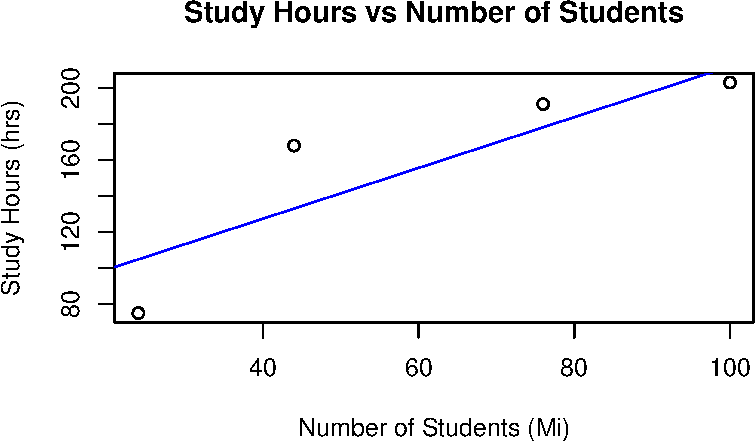
\includegraphics[keepaspectratio]{ups_files/figure-pdf/studyhrs-data-1.pdf}}

\textbf{Estimate the total and mean study hours:}

\begin{table}
\caption*{
{\fontsize{20}{25}\selectfont  SRS Mean Estimation: Working Table\fontsize{12}{15}\selectfont } \\ 
{\fontsize{14}{17}\selectfont  \(n = 5\)\fontsize{12}{15}\selectfont }
} 
\fontsize{12.0pt}{14.0pt}\selectfont
\begin{tabular*}{\linewidth}{@{\extracolsep{\fill}}>{\raggedright\arraybackslash}p{\dimexpr 30.00pt -2\tabcolsep-1.5\arrayrulewidth}>{\raggedleft\arraybackslash}p{\dimexpr 82.50pt -2\tabcolsep-1.5\arrayrulewidth}>{\raggedleft\arraybackslash}p{\dimexpr 82.50pt -2\tabcolsep-1.5\arrayrulewidth}>{\raggedleft\arraybackslash}p{\dimexpr 82.50pt -2\tabcolsep-1.5\arrayrulewidth}}
\toprule
\(i\) & \(t_i/\psi_i\) & \(t_i/\psi_i-\bar y\) & \((t_i/\psi_i-\bar y)^2\)\textsuperscript{\textit{1}} \\ 
\midrule\addlinespace[2.5pt]
1 & 2,021.875 & 2.729 $\times$ 10\textsuperscript{2} & 7.445 $\times$ 10\textsuperscript{4} \\ 
2 & 1,313.410 & -4.356 $\times$ 10\textsuperscript{2} & 1.898 $\times$ 10\textsuperscript{5} \\ 
3 & 1,313.410 & -4.356 $\times$ 10\textsuperscript{2} & 1.898 $\times$ 10\textsuperscript{5} \\ 
4 & 1,626.013 & -1.230 $\times$ 10\textsuperscript{2} & 1.513 $\times$ 10\textsuperscript{4} \\ 
5 & 2,470.364 & 7.213 $\times$ 10\textsuperscript{2} & 5.203 $\times$ 10\textsuperscript{5} \\ 
{\bfseries Sum} & {\bfseries 8,745.072} & {\bfseries -4.547 $\times$ 10\textsuperscript{-13}} & {\bfseries 9.894 $\times$ 10\textsuperscript{5}} \\ 
\bottomrule
\end{tabular*}
\begin{minipage}{\linewidth}
\vspace{.05em}
\textsuperscript{\textit{1}}\(s_y^2 = \sum_i (t_i/\psi_i-\bar y)^2/(n-1) = 247357.3300\).\\
\textbf{Point estimate:} \(\bar y = \dfrac{\sum_i t_i/\psi_i}{n} = \dfrac{8,745.072}{5} = 1,749.014\)\\
\textbf{Standard error:} \(\mathrm{SE}(\bar y) = \dfrac{s}{\sqrt n} = \dfrac{497.350}{\sqrt{5}} = 222.422\)\\
\end{minipage}
\end{table}

\begin{table}
\fontsize{12.0pt}{14.0pt}\selectfont
\begin{tabular*}{0.7\linewidth}{@{\extracolsep{\fill}}rrrr}
\toprule
\(\hat{t}\) & \(\mathrm{SE}(\hat{t})\) & 95\% CI Lower & 95\% CI Upper \\ 
\midrule\addlinespace[2.5pt]
1,749.0144 & 222.4218 & 1,131.4724 & 2,366.5563 \\ 
\bottomrule
\end{tabular*}
\end{table}

\begin{table}
\fontsize{12.0pt}{14.0pt}\selectfont
\begin{tabular*}{0.7\linewidth}{@{\extracolsep{\fill}}rrrr}
\toprule
\(\bar{y}\) & \(\mathrm{SE}(\bar{y})\) & 95\% CI Lower & 95\% CI Upper \\ 
\midrule\addlinespace[2.5pt]
2.7033 & 0.3438 & 1.7488 & 3.6577 \\ 
\bottomrule
\end{tabular*}
\end{table}

\begin{table}
\caption*{
{\fontsize{20}{25}\selectfont  Ratio Estimation: Working Table\fontsize{12}{15}\selectfont } \\ 
{\fontsize{14}{17}\selectfont  \(n = 5\)\fontsize{12}{15}\selectfont }
} 
\fontsize{12.0pt}{14.0pt}\selectfont
\begin{tabular*}{\linewidth}{@{\extracolsep{\fill}}>{\raggedright\arraybackslash}p{\dimexpr 30.00pt -2\tabcolsep-1.5\arrayrulewidth}>{\raggedleft\arraybackslash}p{\dimexpr 75.00pt -2\tabcolsep-1.5\arrayrulewidth}>{\raggedleft\arraybackslash}p{\dimexpr 75.00pt -2\tabcolsep-1.5\arrayrulewidth}>{\raggedleft\arraybackslash}p{\dimexpr 75.00pt -2\tabcolsep-1.5\arrayrulewidth}>{\raggedleft\arraybackslash}p{\dimexpr 75.00pt -2\tabcolsep-1.5\arrayrulewidth}>{\raggedleft\arraybackslash}p{\dimexpr 75.00pt -2\tabcolsep-1.5\arrayrulewidth}}
\toprule
\(i\) & \(t_i/\psi_i\) & \(M_i/\psi_i\) & \(\hat B\,M_i/\psi_i\)\textsuperscript{\textit{1}} & \(e_i\) & \(e_i^2\) \\ 
\midrule\addlinespace[2.5pt]
1 & 2,021.875 & 647.000 & 1,749.014 & 2.729 $\times$ 10\textsuperscript{2} & 7.445 $\times$ 10\textsuperscript{4} \\ 
2 & 1,313.410 & 647.000 & 1,749.014 & -4.356 $\times$ 10\textsuperscript{2} & 1.898 $\times$ 10\textsuperscript{5} \\ 
3 & 1,313.410 & 647.000 & 1,749.014 & -4.356 $\times$ 10\textsuperscript{2} & 1.898 $\times$ 10\textsuperscript{5} \\ 
4 & 1,626.013 & 647.000 & 1,749.014 & -1.230 $\times$ 10\textsuperscript{2} & 1.513 $\times$ 10\textsuperscript{4} \\ 
5 & 2,470.364 & 647.000 & 1,749.014 & 7.213 $\times$ 10\textsuperscript{2} & 5.203 $\times$ 10\textsuperscript{5} \\ 
{\bfseries Sum} & {\bfseries 8,745.072} & {\bfseries 3,235.000} & {\bfseries 8,745.072} & {\bfseries -4.547 $\times$ 10\textsuperscript{-13}} & {\bfseries 9.894 $\times$ 10\textsuperscript{5}} \\ 
\bottomrule
\end{tabular*}
\begin{minipage}{\linewidth}
\vspace{.05em}
\textsuperscript{\textit{1}}\(\hat B = \sum_i t_i/\psi_i / \sum_i M_i/\psi_i = 2.7033\), \(\hat B\,M_i/\psi_i = \hat B\, M_i/\psi_i\), \(s_e^2 = 247357.3300\).\\
\textbf{Point estimate:} \(\hat B = \dfrac{\sum_i t_i/\psi_i}{\sum_i M_i/\psi_i} = \dfrac{8,745.072}{3,235.000} = 2.703\)\\
\textbf{Standard error:} \(\mathrm{SE}(\hat B) = \dfrac{1}{\bar x}\sqrt{\dfrac{s_e^2}{n}} = \dfrac{1}{647.000}\sqrt{\dfrac{2.474 \times 10^{5}}{5}} = 0.344\)\\
\end{minipage}
\end{table}

\begin{table}
\fontsize{12.0pt}{14.0pt}\selectfont
\begin{tabular*}{0.7\linewidth}{@{\extracolsep{\fill}}rrrr}
\toprule
\(\bar{y}_{r}\) & \(\mathrm{SE}(\bar{y}_{r})\) & 95\% CI Lower & 95\% CI Upper \\ 
\midrule\addlinespace[2.5pt]
2.7033 & 0.3438 & 1.7488 & 3.6577 \\ 
\bottomrule
\end{tabular*}
\end{table}

\section{\texorpdfstring{Analysis of \texttt{statepop.csv} collected
with one-stage
UPSWR}{Analysis of statepop.csv collected with one-stage UPSWR}}\label{analysis-of-statepop.csv-collected-with-one-stage-upswr}

The file \texttt{statepop.csv} contains data from an unequal-probability
sample of 100 U.S. counties. Counties were chosen with probabilities
proportional to their populations. The total U.S. population is
\(M_0 = 255,077,536\). Because sampling was done \textbf{with
replacement}, large counties like Los Angeles occur multiple times in
the sample.

\begin{table}
\caption*{
{\fontsize{20}{25}\selectfont  U.S. County Data (Sample)\fontsize{12}{15}\selectfont }
} 
\fontsize{12.0pt}{14.0pt}\selectfont
\begin{tabular*}{\linewidth}{@{\extracolsep{\fill}}llrrr}
\toprule
state & county & popn & phys & psi \\ 
\midrule\addlinespace[2.5pt]
AL & Wilcox & 13672 & 4 & 5.359939e-05 \\ 
AZ & Maricopa & 2209567 & 4320 & 8.662335e-03 \\ 
AZ & Maricopa & 2209567 & 4320 & 8.662335e-03 \\ 
AZ & Pinal & 120786 & 61 & 4.735266e-04 \\ 
AR & Garland & 76100 & 131 & 2.983407e-04 \\ 
AR & Mississippi & 55060 & 48 & 2.158559e-04 \\ 
CA & Contra\_Costa & 840585 & 1761 & 3.295410e-03 \\ 
CA & Kern & 587680 & 682 & 2.303927e-03 \\ 
CA & Los\_Angeles & 9053645 & 23677 & 3.549370e-02 \\ 
CA & Los\_Angeles & 9053645 & 23677 & 3.549370e-02 \\ 
CA & Los\_Angeles & 9053645 & 23677 & 3.549370e-02 \\ 
CA & Los\_Angeles & 9053645 & 23677 & 3.549370e-02 \\ 
CA & Merced & 189107 & 185 & 7.413707e-04 \\ 
CA & Orange & 2484789 & 6062 & 9.741309e-03 \\ 
CA & Riverside & 1288435 & 1385 & 5.051150e-03 \\ 
CA & San\_Francisco & 728921 & 4761 & 2.857645e-03 \\ 
CA & Ventura & 686560 & 1168 & 2.691574e-03 \\ 
CO & Arapahoe & 420882 & 583 & 1.650016e-03 \\ 
FL & Alachua & 189409 & 1180 & 7.425546e-04 \\ 
FL & Lee & 352051 & 509 & 1.380172e-03 \\ 
FL & Orange & 714579 & 1367 & 2.801419e-03 \\ 
FL & Pinellas & 854976 & 1620 & 3.351828e-03 \\ 
GA & Forsyth & 49859 & 21 & 1.954661e-04 \\ 
IL & Cook & 5139341 & 15153 & 2.014815e-02 \\ 
IL & Cook & 5139341 & 15153 & 2.014815e-02 \\ 
IL & Cook & 5139341 & 15153 & 2.014815e-02 \\ 
IL & DuPage & 816116 & 2157 & 3.199482e-03 \\ 
IL & Kane & 333626 & 473 & 1.307940e-03 \\ 
IL & Kane & 333626 & 473 & 1.307940e-03 \\ 
IL & Lake & 541047 & 1093 & 2.121108e-03 \\ 
IL & St.\_Clair & 263124 & 329 & 1.031545e-03 \\ 
IL & Williamson & 58449 & 63 & 2.291421e-04 \\ 
IN & Bartholomew & 65498 & 102 & 2.567768e-04 \\ 
KS & Douglas & 84538 & 107 & 3.314208e-04 \\ 
KY & Boone & 63107 & 62 & 2.474032e-04 \\ 
KY & Jefferson & 670837 & 2171 & 2.629934e-03 \\ 
KY & Jefferson & 670837 & 2171 & 2.629934e-03 \\ 
LA & Jefferson & 457738 & 1237 & 1.794505e-03 \\ 
LA & St.\_Charles & 44372 & 18 & 1.739549e-04 \\ 
MD & Frederick & 159738 & 172 & 6.262331e-04 \\ 
MD & Worcester & 37306 & 24 & 1.462536e-04 \\ 
MI & Oakland & 1118611 & 4020 & 4.385376e-03 \\ 
MI & Oakland & 1118611 & 4020 & 4.385376e-03 \\ 
MN & Hennepin & 1041332 & 3706 & 4.082414e-03 \\ 
MN & Otter\_Tail & 51362 & 55 & 2.013584e-04 \\ 
MS & Leflore & 37477 & 42 & 1.469240e-04 \\ 
MS & Pearl\_River & 39879 & 22 & 1.563407e-04 \\ 
MO & Jasper & 91895 & 135 & 3.602630e-04 \\ 
MO & Nodaway & 21236 & 15 & 8.325312e-05 \\ 
NE & Lancaster & 219582 & 389 & 8.608441e-04 \\ 
NJ & Atlantic & 229430 & 379 & 8.994520e-04 \\ 
NJ & Burlington & 397631 & 719 & 1.558863e-03 \\ 
NJ & Camden & 507735 & 1255 & 1.990512e-03 \\ 
NM & Lea & 56659 & 40 & 2.221246e-04 \\ 
NM & Santa\_Fe & 105178 & 235 & 4.123374e-04 \\ 
NY & Kings & 2286167 & 4861 & 8.962636e-03 \\ 
NY & Kings & 2286167 & 4861 & 8.962636e-03 \\ 
NY & Kings & 2286167 & 4861 & 8.962636e-03 \\ 
NY & Monroe & 724418 & 2438 & 2.839991e-03 \\ 
NY & Nassau & 1302067 & 6147 & 5.104593e-03 \\ 
NY & New\_York & 1489066 & 14052 & 5.837699e-03 \\ 
NY & New\_York & 1489066 & 14052 & 5.837699e-03 \\ 
NY & Richmond & 391085 & 1242 & 1.533200e-03 \\ 
NY & Richmond & 391085 & 1242 & 1.533200e-03 \\ 
NY & Saratoga & 188387 & 215 & 7.385480e-04 \\ 
NY & Suffolk & 1338204 & 3021 & 5.246264e-03 \\ 
NY & Suffolk & 1338204 & 3021 & 5.246264e-03 \\ 
NC & Rutherford & 57951 & 46 & 2.271897e-04 \\ 
OH & Allen & 26405 & 168 & 1.035175e-04 \\ 
OH & Cuyahoga & 1411209 & 5620 & 5.532471e-03 \\ 
OH & Franklin & 992095 & 2675 & 3.889386e-03 \\ 
OH & Hamilton & 872026 & 3164 & 3.418670e-03 \\ 
OH & Harrison & 15946 & 12 & 6.251433e-05 \\ 
OH & Lucas & 461508 & 1391 & 1.809285e-03 \\ 
OH & Stark & 372125 & 595 & 1.458870e-03 \\ 
OK & Tulsa & 519847 & 1158 & 2.037996e-03 \\ 
OR & Multnomah & 600811 & 2571 & 2.355405e-03 \\ 
OR & Wasco & 22219 & 44 & 8.710685e-05 \\ 
PA & Allegheny & 1334396 & 5281 & 5.231335e-03 \\ 
PA & Allegheny & 1334396 & 5281 & 5.231335e-03 \\ 
PA & Bucks & 556279 & 879 & 2.180823e-03 \\ 
PA & Delaware & 549506 & 1374 & 2.154270e-03 \\ 
PA & Luzerne & 328927 & 594 & 1.289518e-03 \\ 
PA & Northampton & 252393 & 459 & 9.894756e-04 \\ 
SC & Greenville & 324558 & 650 & 1.272390e-03 \\ 
SD & Charles\_Mix & 9265 & 6 & 3.632229e-05 \\ 
TN & Coffee & 41641 & 50 & 1.632484e-04 \\ 
TN & Dickson & 36509 & 27 & 1.431290e-04 \\ 
TN & Hamblen & 51657 & 54 & 2.025149e-04 \\ 
TN & Shelby & 844847 & 2489 & 3.312118e-03 \\ 
TN & Sullivan & 146676 & 377 & 5.750252e-04 \\ 
TX & Cooke & 30948 & 21 & 1.213278e-04 \\ 
TX & Ector & 122338 & 153 & 4.796110e-04 \\ 
TX & Fort\_Bend & 255788 & 231 & 1.002785e-03 \\ 
TX & Wichita & 120386 & 243 & 4.719585e-04 \\ 
UT & Davis & 199953 & 166 & 7.838911e-04 \\ 
VA & Chesterfield & 225225 & 181 & 8.829668e-04 \\ 
WA & King & 1557537 & 5280 & 6.106132e-03 \\ 
WI & Lincoln & 27822 & 28 & 1.090727e-04 \\ 
WI & Waukesha & 320306 & 687 & 1.255720e-03 \\ 
\bottomrule
\end{tabular*}
\end{table}

\pandocbounded{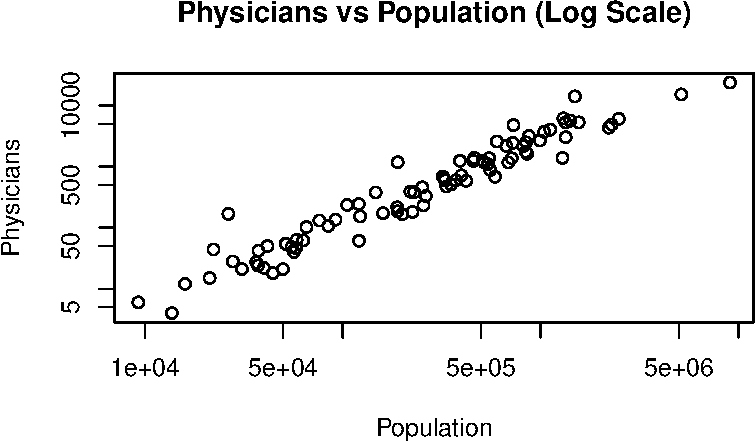
\includegraphics[keepaspectratio]{ups_files/figure-pdf/statepop-load-1.pdf}}

\textbf{Estimate the Total and Per Capita Physicians:}

\begin{table}
\fontsize{12.0pt}{14.0pt}\selectfont
\begin{tabular*}{0.7\linewidth}{@{\extracolsep{\fill}}rrrr}
\toprule
\(\hat{t}\) & \(\mathrm{SE}(\hat{t})\) & 95\% CI Lower & 95\% CI Upper \\ 
\midrule\addlinespace[2.5pt]
570,304.2951 & 41,401.2299 & 488,155.2729 & 652,453.3173 \\ 
\bottomrule
\end{tabular*}
\end{table}

\begin{table}
\caption*{
{\fontsize{20}{25}\selectfont  Ratio Estimation: Working Table\fontsize{12}{15}\selectfont } \\ 
{\fontsize{14}{17}\selectfont  \(n = 100\)\fontsize{12}{15}\selectfont }
} 
\fontsize{12.0pt}{14.0pt}\selectfont
\begin{tabular*}{\linewidth}{@{\extracolsep{\fill}}>{\raggedright\arraybackslash}p{\dimexpr 30.00pt -2\tabcolsep-1.5\arrayrulewidth}>{\raggedleft\arraybackslash}p{\dimexpr 75.00pt -2\tabcolsep-1.5\arrayrulewidth}>{\raggedleft\arraybackslash}p{\dimexpr 75.00pt -2\tabcolsep-1.5\arrayrulewidth}>{\raggedleft\arraybackslash}p{\dimexpr 75.00pt -2\tabcolsep-1.5\arrayrulewidth}>{\raggedleft\arraybackslash}p{\dimexpr 75.00pt -2\tabcolsep-1.5\arrayrulewidth}>{\raggedleft\arraybackslash}p{\dimexpr 75.00pt -2\tabcolsep-1.5\arrayrulewidth}}
\toprule
\(i\) & \(t_i/\psi_i\) & \(M_i/\psi_i\) & \(\hat B\,M_i/\psi_i\)\textsuperscript{\textit{1}} & \(e_i\) & \(e_i^2\) \\ 
\midrule\addlinespace[2.5pt]
1 & 7.463 $\times$ 10\textsuperscript{4} & 2.551 $\times$ 10\textsuperscript{8} & 5.703 $\times$ 10\textsuperscript{5} & -4.957 $\times$ 10\textsuperscript{5} & 2.457 $\times$ 10\textsuperscript{11} \\ 
2 & 4.987 $\times$ 10\textsuperscript{5} & 2.551 $\times$ 10\textsuperscript{8} & 5.703 $\times$ 10\textsuperscript{5} & -7.159 $\times$ 10\textsuperscript{4} & 5.126 $\times$ 10\textsuperscript{9} \\ 
3 & 4.987 $\times$ 10\textsuperscript{5} & 2.551 $\times$ 10\textsuperscript{8} & 5.703 $\times$ 10\textsuperscript{5} & -7.159 $\times$ 10\textsuperscript{4} & 5.126 $\times$ 10\textsuperscript{9} \\ 
4 & 1.288 $\times$ 10\textsuperscript{5} & 2.551 $\times$ 10\textsuperscript{8} & 5.703 $\times$ 10\textsuperscript{5} & -4.415 $\times$ 10\textsuperscript{5} & 1.949 $\times$ 10\textsuperscript{11} \\ 
5 & 4.391 $\times$ 10\textsuperscript{5} & 2.551 $\times$ 10\textsuperscript{8} & 5.703 $\times$ 10\textsuperscript{5} & -1.312 $\times$ 10\textsuperscript{5} & 1.722 $\times$ 10\textsuperscript{10} \\ 
6 & 2.224 $\times$ 10\textsuperscript{5} & 2.551 $\times$ 10\textsuperscript{8} & 5.703 $\times$ 10\textsuperscript{5} & -3.479 $\times$ 10\textsuperscript{5} & 1.211 $\times$ 10\textsuperscript{11} \\ 
... & ... & ... & ... & ... & ... \\ 
{\bfseries Sum} & {\bfseries 5.703 $\times$ 10\textsuperscript{7}} & {\bfseries 2.551 $\times$ 10\textsuperscript{10}} & {\bfseries 5.703 $\times$ 10\textsuperscript{7}} & {\bfseries -2.095 $\times$ 10\textsuperscript{-9}} & {\bfseries 1.697 $\times$ 10\textsuperscript{13}} \\ 
\bottomrule
\end{tabular*}
\begin{minipage}{\linewidth}
\vspace{.05em}
\textsuperscript{\textit{1}}\(\hat B = \sum_i t_i/\psi_i / \sum_i M_i/\psi_i = 0.0022\), \(\hat B\,M_i/\psi_i = \hat B\, M_i/\psi_i\), \(s_e^2 = 171406183906.6202\).\\
\textbf{Point estimate:} \(\hat B = \dfrac{\sum_i t_i/\psi_i}{\sum_i M_i/\psi_i} = \dfrac{5.703 \times 10^{7}}{2.551 \times 10^{10}} = 0.002\)\\
\textbf{Standard error:} \(\mathrm{SE}(\hat B) = \dfrac{1}{\bar x}\sqrt{\dfrac{s_e^2}{n}} = \dfrac{1}{2.551 \times 10^{8}}\sqrt{\dfrac{1.714 \times 10^{11}}{100}} = 1.623 \times 10^{-4}\)\\
\end{minipage}
\end{table}

\begin{table}
\fontsize{12.0pt}{14.0pt}\selectfont
\begin{tabular*}{0.7\linewidth}{@{\extracolsep{\fill}}rrrr}
\toprule
\(\bar{y}_{r}\) & \(\mathrm{SE}(\bar{y}_{r})\) & 95\% CI Lower & 95\% CI Upper \\ 
\midrule\addlinespace[2.5pt]
0.0022 & 0.0002 & 0.0019 & 0.0026 \\ 
\bottomrule
\end{tabular*}
\end{table}

\textbf{Output Note:} The total estimator heavily leverages the
selection probabilities to estimate that there are roughly
\ensuremath{5.70304\times 10^{5}} physicians in the US.

\subsection{Compare with an estimate based on an SRS
sample}\label{compare-with-an-estimate-based-on-an-srs-sample}

Let's compare our UPSWR results against a naive Simple Random Sample of
100 counties.

\begin{table}
\fontsize{12.0pt}{14.0pt}\selectfont
\begin{tabular*}{0.7\linewidth}{@{\extracolsep{\fill}}rrrr}
\toprule
\(\hat{t}\) & \(\mathrm{SE}(\hat{t})\) & 95\% CI Lower & 95\% CI Upper \\ 
\midrule\addlinespace[2.5pt]
933,410.9700 & 491,982.7871 & -42,789.6161 & 1,909,611.5561 \\ 
\bottomrule
\end{tabular*}
\end{table}

\begin{table}
\caption*{
{\fontsize{20}{25}\selectfont  Ratio Estimation: Working Table\fontsize{12}{15}\selectfont } \\ 
{\fontsize{14}{17}\selectfont  \(n = 100\)\fontsize{12}{15}\selectfont }
} 
\fontsize{12.0pt}{14.0pt}\selectfont
\begin{tabular*}{\linewidth}{@{\extracolsep{\fill}}>{\raggedright\arraybackslash}p{\dimexpr 30.00pt -2\tabcolsep-1.5\arrayrulewidth}>{\raggedleft\arraybackslash}p{\dimexpr 75.00pt -2\tabcolsep-1.5\arrayrulewidth}>{\raggedleft\arraybackslash}p{\dimexpr 75.00pt -2\tabcolsep-1.5\arrayrulewidth}>{\raggedleft\arraybackslash}p{\dimexpr 75.00pt -2\tabcolsep-1.5\arrayrulewidth}>{\raggedleft\arraybackslash}p{\dimexpr 75.00pt -2\tabcolsep-1.5\arrayrulewidth}>{\raggedleft\arraybackslash}p{\dimexpr 75.00pt -2\tabcolsep-1.5\arrayrulewidth}}
\toprule
\(i\) & \(y_i\) & \(x_i\) & \(\hat y_i\)\textsuperscript{\textit{1}} & \(e_i\) & \(e_i^2\) \\ 
\midrule\addlinespace[2.5pt]
1 & 24.000 & 3.602 $\times$ 10\textsuperscript{4} & 90.313 & -6.631 $\times$ 10\textsuperscript{1} & 4.397 $\times$ 10\textsuperscript{3} \\ 
2 & 44.000 & 7.352 $\times$ 10\textsuperscript{4} & 184.332 & -1.403 $\times$ 10\textsuperscript{2} & 1.969 $\times$ 10\textsuperscript{4} \\ 
3 & 7.000 & 6.408 $\times$ 10\textsuperscript{3} & 16.066 & -9.066 & 8.218 $\times$ 10\textsuperscript{1} \\ 
4 & 11.000 & 1.926 $\times$ 10\textsuperscript{4} & 48.289 & -3.729 $\times$ 10\textsuperscript{1} & 1.390 $\times$ 10\textsuperscript{3} \\ 
5 & 3.000 & 7.649 $\times$ 10\textsuperscript{3} & 19.177 & -1.618 $\times$ 10\textsuperscript{1} & 2.617 $\times$ 10\textsuperscript{2} \\ 
6 & 327.000 & 1.884 $\times$ 10\textsuperscript{5} & 472.281 & -1.453 $\times$ 10\textsuperscript{2} & 2.111 $\times$ 10\textsuperscript{4} \\ 
... & ... & ... & ... & ... & ... \\ 
{\bfseries Sum} & {\bfseries 29,717.000} & {\bfseries 1.185 $\times$ 10\textsuperscript{7}} & {\bfseries 29,717.000} & {\bfseries -2.675 $\times$ 10\textsuperscript{-12}} & {\bfseries 1.705 $\times$ 10\textsuperscript{7}} \\ 
\bottomrule
\end{tabular*}
\begin{minipage}{\linewidth}
\vspace{.05em}
\textsuperscript{\textit{1}}\(\hat B = \sum_i y_i / \sum_i x_i = 0.0025\), \(\hat y_i = \hat B\, x_i\), \(s_e^2 = 172267.8740\).\\
\textbf{Point estimate:} \(\hat t = \hat B\,\bar x_U\,N = 0.003 \times 81,209.021 \times 3,141 = 6.395 \times 10^{5}\)\\
\textbf{Standard error:} \(\mathrm{SE}(\hat t) = \mathrm{SE}(\hat B)\,\bar x_U\,N = 3.445 \times 10^{-4} \times 81,209.021 \times 3,141 = 87,885.265\)\\
\end{minipage}
\end{table}

\begin{table}
\fontsize{12.0pt}{14.0pt}\selectfont
\begin{tabular*}{0.7\linewidth}{@{\extracolsep{\fill}}rrrr}
\toprule
\(\hat{t}\) & \(\mathrm{SE}(\hat{t})\) & 95\% CI Lower & 95\% CI Upper \\ 
\midrule\addlinespace[2.5pt]
639,506.0284 & 87,885.2651 & 465,122.5955 & 813,889.4613 \\ 
\bottomrule
\end{tabular*}
\end{table}

\begin{table}
\caption*{
{\fontsize{20}{25}\selectfont  Regression Estimation: Working Table\fontsize{12}{15}\selectfont } \\ 
{\fontsize{14}{17}\selectfont  \(n = 100\)\fontsize{12}{15}\selectfont }
} 
\fontsize{12.0pt}{14.0pt}\selectfont
\begin{tabular*}{\linewidth}{@{\extracolsep{\fill}}>{\raggedright\arraybackslash}p{\dimexpr 30.00pt -2\tabcolsep-1.5\arrayrulewidth}>{\raggedleft\arraybackslash}p{\dimexpr 75.00pt -2\tabcolsep-1.5\arrayrulewidth}>{\raggedleft\arraybackslash}p{\dimexpr 75.00pt -2\tabcolsep-1.5\arrayrulewidth}>{\raggedleft\arraybackslash}p{\dimexpr 75.00pt -2\tabcolsep-1.5\arrayrulewidth}>{\raggedleft\arraybackslash}p{\dimexpr 75.00pt -2\tabcolsep-1.5\arrayrulewidth}>{\raggedleft\arraybackslash}p{\dimexpr 75.00pt -2\tabcolsep-1.5\arrayrulewidth}}
\toprule
\(i\) & \(y_i\) & \(x_i\) & \(\hat y_i\)\textsuperscript{\textit{1}} & \(e_i\) & \(e_i^2\) \\ 
\midrule\addlinespace[2.5pt]
1 & 24.000 & 3.602 $\times$ 10\textsuperscript{4} & 52.564 & -2.856 $\times$ 10\textsuperscript{1} & 8.159 $\times$ 10\textsuperscript{2} \\ 
2 & 44.000 & 7.352 $\times$ 10\textsuperscript{4} & 163.740 & -1.197 $\times$ 10\textsuperscript{2} & 1.434 $\times$ 10\textsuperscript{4} \\ 
3 & 7.000 & 6.408 $\times$ 10\textsuperscript{3} & -35.234 & 4.223 $\times$ 10\textsuperscript{1} & 1.784 $\times$ 10\textsuperscript{3} \\ 
4 & 11.000 & 1.926 $\times$ 10\textsuperscript{4} & 2.871 & 8.129 & 6.609 $\times$ 10\textsuperscript{1} \\ 
5 & 3.000 & 7.649 $\times$ 10\textsuperscript{3} & -31.555 & 3.455 $\times$ 10\textsuperscript{1} & 1.194 $\times$ 10\textsuperscript{3} \\ 
6 & 327.000 & 1.884 $\times$ 10\textsuperscript{5} & 504.237 & -1.772 $\times$ 10\textsuperscript{2} & 3.141 $\times$ 10\textsuperscript{4} \\ 
... & ... & ... & ... & ... & ... \\ 
{\bfseries Sum} & {\bfseries 29,717.000} & {\bfseries 1.185 $\times$ 10\textsuperscript{7}} & {\bfseries 29,717.000} & {\bfseries 6.963 $\times$ 10\textsuperscript{-13}} & {\bfseries 1.135 $\times$ 10\textsuperscript{7}} \\ 
\bottomrule
\end{tabular*}
\begin{minipage}{\linewidth}
\vspace{.05em}
\textsuperscript{\textit{1}}\(\hat B_0 = -54.2313\), \(\hat B_1 = 0.0030\), \(\hat y_i = \hat B_0 + \hat B_1 x_i\), \(s_e^2 = 115813.8922\).\\
\textbf{Point estimate:} \(\hat t_{reg} = N\bar y_{reg} = 3,141 \times 186.524 = 5.859 \times 10^{5}\)\\
\textbf{Standard error:} \(\mathrm{SE}(\hat t_{reg}) = N\times\mathrm{SE}(\bar y_{reg}) = 3,141 \times 33.485 = 1.052 \times 10^{5}\)\\
\end{minipage}
\end{table}

\begin{table}
\fontsize{12.0pt}{14.0pt}\selectfont
\begin{tabular*}{0.7\linewidth}{@{\extracolsep{\fill}}rrrr}
\toprule
\(\hat{t}_{reg}\) & \(\mathrm{SE}(\hat{t}_{reg})\) & 95\% CI Lower & 95\% CI Upper \\ 
\midrule\addlinespace[2.5pt]
585,870.5992 & 105,177.4184 & 377,149.4353 & 794,591.7630 \\ 
\bottomrule
\end{tabular*}
\end{table}

\textbf{Output Note:} The true value is \textbf{532,638}. Notice how
poorly the naive SRS estimate performs (predicting over 800,000) because
it ignores county sizes. Both the SRS Ratio and SRS Regression methods
perform much better by incorporating auxiliary population data.

\section{\texorpdfstring{Analysis of \texttt{studenthrs.csv} collected
with two-stage
UPSWR}{Analysis of studenthrs.csv collected with two-stage UPSWR}}\label{analysis-of-studenthrs.csv-collected-with-two-stage-upswr}

Here, we sample classes (Primary Sampling Units) with replacement based
on class size, and then subsample students within them to ask about
their study hours.

\begin{table}
\caption*{
{\fontsize{20}{25}\selectfont  Ratio Estimation: Working Table\fontsize{12}{15}\selectfont } \\ 
{\fontsize{14}{17}\selectfont  \(n = 5\)\fontsize{12}{15}\selectfont }
} 
\fontsize{12.0pt}{14.0pt}\selectfont
\begin{tabular*}{\linewidth}{@{\extracolsep{\fill}}>{\raggedright\arraybackslash}p{\dimexpr 30.00pt -2\tabcolsep-1.5\arrayrulewidth}>{\raggedleft\arraybackslash}p{\dimexpr 75.00pt -2\tabcolsep-1.5\arrayrulewidth}>{\raggedleft\arraybackslash}p{\dimexpr 75.00pt -2\tabcolsep-1.5\arrayrulewidth}>{\raggedleft\arraybackslash}p{\dimexpr 75.00pt -2\tabcolsep-1.5\arrayrulewidth}>{\raggedleft\arraybackslash}p{\dimexpr 75.00pt -2\tabcolsep-1.5\arrayrulewidth}>{\raggedleft\arraybackslash}p{\dimexpr 75.00pt -2\tabcolsep-1.5\arrayrulewidth}}
\toprule
\(i\) & \(t_i/\psi_i\) & \(M_i/\psi_i\) & \(\hat B\,M_i/\psi_i\)\textsuperscript{\textit{1}} & \(e_i\) & \(e_i^2\) \\ 
\midrule\addlinespace[2.5pt]
1 & 2,393.900 & 647.000 & 1,617.500 & 776.400 & 6.028 $\times$ 10\textsuperscript{5} \\ 
2 & 1,811.600 & 647.000 & 1,617.500 & 194.100 & 3.767 $\times$ 10\textsuperscript{4} \\ 
3 & 1,552.800 & 647.000 & 1,617.500 & -64.700 & 4.186 $\times$ 10\textsuperscript{3} \\ 
4 & 1,035.200 & 647.000 & 1,617.500 & -582.300 & 3.391 $\times$ 10\textsuperscript{5} \\ 
5 & 1,294.000 & 647.000 & 1,617.500 & -323.500 & 1.047 $\times$ 10\textsuperscript{5} \\ 
{\bfseries Sum} & {\bfseries 8,087.500} & {\bfseries 3,235.000} & {\bfseries 8,087.500} & {\bfseries 0.000} & {\bfseries 1.088 $\times$ 10\textsuperscript{6}} \\ 
\bottomrule
\end{tabular*}
\begin{minipage}{\linewidth}
\vspace{.05em}
\textsuperscript{\textit{1}}\(\hat B = \sum_i t_i/\psi_i / \sum_i M_i/\psi_i = 2.5000\), \(\hat B\,M_i/\psi_i = \hat B\, M_i/\psi_i\), \(s_e^2 = 272095.8500\).\\
\textbf{Point estimate:} \(\hat B = \dfrac{\sum_i t_i/\psi_i}{\sum_i M_i/\psi_i} = \dfrac{8,087.500}{3,235.000} = 2.500\)\\
\textbf{Standard error:} \(\mathrm{SE}(\hat B) = \dfrac{1}{\bar x}\sqrt{\dfrac{s_e^2}{n}} = \dfrac{1}{647.000}\sqrt{\dfrac{2.721 \times 10^{5}}{5}} = 0.361\)\\
\end{minipage}
\end{table}

\textbf{Estimate the overall mean study hours:}

\begin{table}
\fontsize{12.0pt}{14.0pt}\selectfont
\begin{tabular*}{0.7\linewidth}{@{\extracolsep{\fill}}rrrr}
\toprule
\(\bar{y}_{r}\) & \(\mathrm{SE}(\bar{y}_{r})\) & 95\% CI Lower & 95\% CI Upper \\ 
\midrule\addlinespace[2.5pt]
2.5000 & 0.3606 & 1.4989 & 3.5011 \\ 
\bottomrule
\end{tabular*}
\end{table}

\section{\texorpdfstring{Simulation Studies for UPSWR using
\texttt{agpop}
data}{Simulation Studies for UPSWR using agpop data}}\label{simulation-studies-for-upswr-using-agpop-data}

Let's simulate 2000 random samples to see how UPSWR empirically compares
to Simple Random Sampling.

\subsection{Visualizing Estimator
Variance}\label{visualizing-estimator-variance}

\pandocbounded{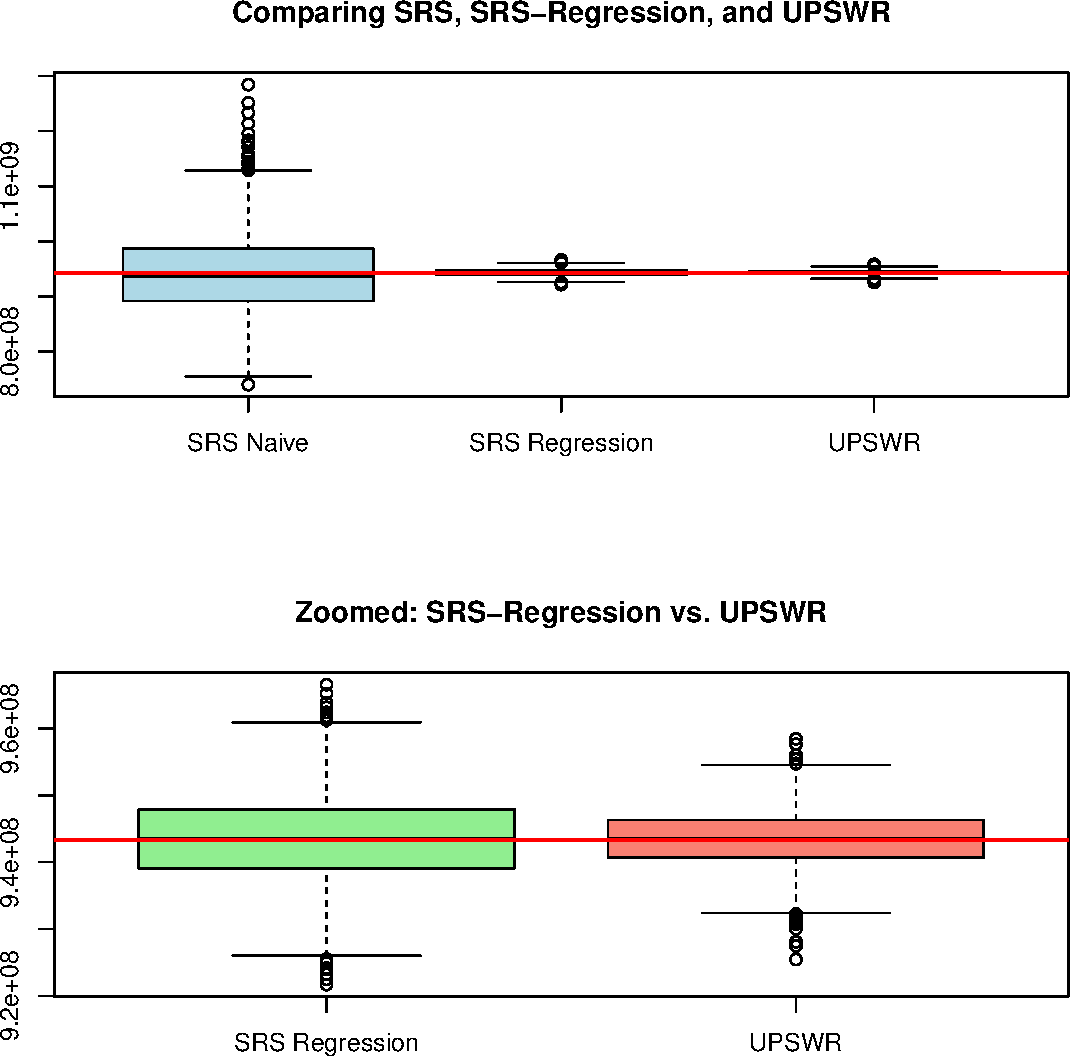
\includegraphics[keepaspectratio]{ups_files/figure-pdf/upswr-sim-plot-1.pdf}}

\textbf{Output Note:} The red line represents the true total acreage.
The naive SRS estimator has massive variance. Both SRS Regression and
UPSWR drastically reduce variance, centering tightly around the true
mean.

\section{Analysis of a dataset on student study hours collected by
UPSWO}\label{analysis-of-a-dataset-on-student-study-hours-collected-by-upswo}

When sampling \textbf{Without Replacement} with unequal probabilities,
we rely on the inclusion probabilities (\(\pi_k\)) rather than
single-draw probabilities (\(\psi_i\)).

\begin{table}
\caption*{
{\fontsize{20}{25}\selectfont  Ratio Estimation: Working Table\fontsize{12}{15}\selectfont } \\ 
{\fontsize{14}{17}\selectfont  \(n = 5\)\fontsize{12}{15}\selectfont }
} 
\fontsize{12.0pt}{14.0pt}\selectfont
\begin{tabular*}{\linewidth}{@{\extracolsep{\fill}}>{\raggedright\arraybackslash}p{\dimexpr 30.00pt -2\tabcolsep-1.5\arrayrulewidth}>{\raggedleft\arraybackslash}p{\dimexpr 75.00pt -2\tabcolsep-1.5\arrayrulewidth}>{\raggedleft\arraybackslash}p{\dimexpr 75.00pt -2\tabcolsep-1.5\arrayrulewidth}>{\raggedleft\arraybackslash}p{\dimexpr 75.00pt -2\tabcolsep-1.5\arrayrulewidth}>{\raggedleft\arraybackslash}p{\dimexpr 75.00pt -2\tabcolsep-1.5\arrayrulewidth}>{\raggedleft\arraybackslash}p{\dimexpr 75.00pt -2\tabcolsep-1.5\arrayrulewidth}}
\toprule
\(i\) & \(\hat t_i/\pi_i\) & \(M_i/\pi_i\) & \(\hat B\,M_i/\pi_i\)\textsuperscript{\textit{1}} & \(e_i\) & \(e_i^2\) \\ 
\midrule\addlinespace[2.5pt]
1 & 3.500 & 1.000 & 3.450 & 5.000 $\times$ 10\textsuperscript{-2} & 0.002 \\ 
2 & 5.000 & 1.000 & 3.450 & 1.550 & 2.402 \\ 
3 & 3.625 & 1.000 & 3.450 & 1.750 $\times$ 10\textsuperscript{-1} & 0.031 \\ 
4 & 3.125 & 1.000 & 3.450 & -3.250 $\times$ 10\textsuperscript{-1} & 0.106 \\ 
5 & 2.000 & 1.000 & 3.450 & -1.450 & 2.103 \\ 
{\bfseries Sum} & {\bfseries 17.250} & {\bfseries 5.000} & {\bfseries 17.250} & {\bfseries -8.882 $\times$ 10\textsuperscript{-16}} & {\bfseries 4.644} \\ 
\bottomrule
\end{tabular*}
\begin{minipage}{\linewidth}
\vspace{.05em}
\textsuperscript{\textit{1}}\(\hat B = \sum_i \hat t_i/\pi_i / \sum_i M_i/\pi_i = 3.4500\), \(\hat B\,M_i/\pi_i = \hat B\, M_i/\pi_i\), \(s_e^2 = 1.1609\).\\
\textbf{Point estimate:} \(\hat B = \dfrac{\sum_i \hat t_i/\pi_i}{\sum_i M_i/\pi_i} = \dfrac{17.250}{5.000} = 3.450\)\\
\textbf{Standard error:} \(\mathrm{SE}(\hat B) = \dfrac{1}{\bar x}\sqrt{\dfrac{s_e^2}{n}} = \dfrac{1}{1.000}\sqrt{\dfrac{1.161}{5}} = 0.482\)\\
\end{minipage}
\end{table}

\textbf{Estimate the overall mean study hours (Horvitz-Thompson ratio
style):}

\begin{table}
\fontsize{12.0pt}{14.0pt}\selectfont
\begin{tabular*}{0.7\linewidth}{@{\extracolsep{\fill}}rrrr}
\toprule
\(\bar{y}_{r}\) & \(\mathrm{SE}(\bar{y}_{r})\) & 95\% CI Lower & 95\% CI Upper \\ 
\midrule\addlinespace[2.5pt]
3.4500 & 0.4819 & 2.1121 & 4.7879 \\ 
\bottomrule
\end{tabular*}
\end{table}

\cleardoublepage
\phantomsection
\addcontentsline{toc}{part}{Appendices}
\appendix

\chapter{Estimating Functions Source
Code}\label{estimating-functions-source-code}

The R functions used throughout this book to compute point estimates,
standard errors, and confidence intervals --- along with their
\texttt{gt}-table formatting helpers --- are defined in a single shared
file, \texttt{samplingestimate.r}, which every chapter sources. Its full
source is listed below for reference.

\begin{Shaded}
\begin{Highlighting}[]
\CommentTok{\# =============================================================}
\CommentTok{\# Shared estimation functions for the Elements of Sampling Survey}
\CommentTok{\# book. Source this file from any chapter that needs point/SE/CI}
\CommentTok{\# estimators or their gt{-}table formatting helpers, e.g.:}
\CommentTok{\#}
\CommentTok{\#   source("samplingestimate.r")}
\CommentTok{\#}
\CommentTok{\# =============================================================}

\FunctionTok{suppressPackageStartupMessages}\NormalTok{(\{}
    \FunctionTok{library}\NormalTok{(gt)}
\NormalTok{\})}

\CommentTok{\# {-}{-}{-}{-}{-}{-}{-}{-}{-}{-}{-}{-}{-}{-}{-}{-}{-}{-}{-}{-}{-}{-}{-}{-}{-}{-}{-}{-}{-}{-}{-}{-}{-}{-}{-}{-}{-}{-}{-}{-}{-}{-}{-}{-}{-}{-}{-}{-}{-}{-}{-}{-}{-}{-}{-}{-}{-}}
\CommentTok{\# Shared gt{-}table helpers}
\CommentTok{\# {-}{-}{-}{-}{-}{-}{-}{-}{-}{-}{-}{-}{-}{-}{-}{-}{-}{-}{-}{-}{-}{-}{-}{-}{-}{-}{-}{-}{-}{-}{-}{-}{-}{-}{-}{-}{-}{-}{-}{-}{-}{-}{-}{-}{-}{-}{-}{-}{-}{-}{-}{-}{-}{-}{-}{-}{-}}

\DocumentationTok{\#\# Formats a gt table column as ordinary fixed{-}point, UNLESS its values are}
\DocumentationTok{\#\# too small (\textless{} \textasciigrave{}small\textasciigrave{} in absolute value) or too large (\textgreater{}= \textasciigrave{}large\textasciigrave{}), in}
\DocumentationTok{\#\# which case it switches that column to scientific notation (rendered as}
\DocumentationTok{\#\# "m x 10\^{}n" via gt\textquotesingle{}s exp\_style = "x10n") instead.}
\NormalTok{fmt\_auto }\OtherTok{\textless{}{-}} \ControlFlowTok{function}\NormalTok{ (gt\_tbl, data, columns, }\AttributeTok{decimals =} \DecValTok{3}\NormalTok{, }\AttributeTok{small =} \FloatTok{1e{-}3}\NormalTok{, }\AttributeTok{large =} \FloatTok{1e5}\NormalTok{)}
\NormalTok{\{}
    \ControlFlowTok{for}\NormalTok{ (col }\ControlFlowTok{in}\NormalTok{ columns)}
\NormalTok{    \{}
\NormalTok{        x }\OtherTok{\textless{}{-}}\NormalTok{ data[[col]]}
\NormalTok{        x }\OtherTok{\textless{}{-}}\NormalTok{ x[}\FunctionTok{is.finite}\NormalTok{ (x) }\SpecialCharTok{\&}\NormalTok{ x }\SpecialCharTok{!=} \DecValTok{0}\NormalTok{]}
        \ControlFlowTok{if}\NormalTok{ (}\FunctionTok{length}\NormalTok{ (x) }\SpecialCharTok{==} \DecValTok{0}\NormalTok{) }\ControlFlowTok{next}
        \ControlFlowTok{if}\NormalTok{ (}\FunctionTok{any}\NormalTok{ (}\FunctionTok{abs}\NormalTok{ (x) }\SpecialCharTok{\textless{}}\NormalTok{ small) }\SpecialCharTok{||} \FunctionTok{any}\NormalTok{ (}\FunctionTok{abs}\NormalTok{ (x) }\SpecialCharTok{\textgreater{}=}\NormalTok{ large))}
\NormalTok{            gt\_tbl }\OtherTok{\textless{}{-}} \FunctionTok{fmt\_scientific}\NormalTok{ (gt\_tbl, }\AttributeTok{columns =}\NormalTok{ tidyselect}\SpecialCharTok{::}\FunctionTok{all\_of}\NormalTok{ (col), }\AttributeTok{decimals =}\NormalTok{ decimals, }\AttributeTok{exp\_style =} \StringTok{"x10n"}\NormalTok{)}
        \ControlFlowTok{else}
\NormalTok{            gt\_tbl }\OtherTok{\textless{}{-}} \FunctionTok{fmt\_number}\NormalTok{ (gt\_tbl, }\AttributeTok{columns =}\NormalTok{ tidyselect}\SpecialCharTok{::}\FunctionTok{all\_of}\NormalTok{ (col), }\AttributeTok{decimals =}\NormalTok{ decimals)}
\NormalTok{    \}}
\NormalTok{    gt\_tbl}
\NormalTok{\}}

\DocumentationTok{\#\# Formats a single scalar for inline formula display (fixed{-}point with}
\DocumentationTok{\#\# thousands separators, switching to "m \textbackslash{}times 10\^{}\{n\}" LaTeX scientific}
\DocumentationTok{\#\# notation for very small or very large magnitudes, mirroring fmt\_auto()\textquotesingle{}s}
\DocumentationTok{\#\# use of exp\_style = "x10n") {-}{-}{-} used to show worked{-}example steps such as}
\DocumentationTok{\#\# \textbackslash{}bar y = sum/n with the actual numbers plugged in.}
\NormalTok{fmt\_num }\OtherTok{\textless{}{-}} \ControlFlowTok{function}\NormalTok{ (x, }\AttributeTok{decimals =} \DecValTok{3}\NormalTok{, }\AttributeTok{small =} \FloatTok{1e{-}3}\NormalTok{, }\AttributeTok{large =} \FloatTok{1e5}\NormalTok{)}
\NormalTok{\{}
\NormalTok{    use\_sci }\OtherTok{\textless{}{-}} \FunctionTok{is.finite}\NormalTok{ (x) }\SpecialCharTok{\&}\NormalTok{ x }\SpecialCharTok{!=} \DecValTok{0} \SpecialCharTok{\&}\NormalTok{ (}\FunctionTok{abs}\NormalTok{ (x) }\SpecialCharTok{\textless{}}\NormalTok{ small }\SpecialCharTok{|} \FunctionTok{abs}\NormalTok{ (x) }\SpecialCharTok{\textgreater{}=}\NormalTok{ large)}
\NormalTok{    exps    }\OtherTok{\textless{}{-}} \FunctionTok{ifelse}\NormalTok{ (x }\SpecialCharTok{==} \DecValTok{0}\NormalTok{, }\DecValTok{0}\NormalTok{, }\FunctionTok{floor}\NormalTok{ (}\FunctionTok{log10}\NormalTok{ (}\FunctionTok{abs}\NormalTok{ (x))))}
\NormalTok{    mant    }\OtherTok{\textless{}{-}} \FunctionTok{ifelse}\NormalTok{ (x }\SpecialCharTok{==} \DecValTok{0}\NormalTok{, }\DecValTok{0}\NormalTok{, x }\SpecialCharTok{/} \DecValTok{10}\SpecialCharTok{\^{}}\NormalTok{exps)}
    \FunctionTok{ifelse}\NormalTok{ (use\_sci,}
            \FunctionTok{sprintf}\NormalTok{ (}\StringTok{"\%s }\SpecialCharTok{\textbackslash{}\textbackslash{}}\StringTok{times 10\^{}\{\%d\}"}\NormalTok{, }\FunctionTok{formatC}\NormalTok{ (mant, }\AttributeTok{format =} \StringTok{"f"}\NormalTok{, }\AttributeTok{digits =}\NormalTok{ decimals), exps),}
            \FunctionTok{formatC}\NormalTok{ (x, }\AttributeTok{format =} \StringTok{"f"}\NormalTok{, }\AttributeTok{digits =}\NormalTok{ decimals, }\AttributeTok{big.mark =} \StringTok{","}\NormalTok{))}
\NormalTok{\}}

\DocumentationTok{\#\# Truncates a row{-}level working data.frame whose LAST row is a summary row}
\DocumentationTok{\#\# (e.g. "Sum"/"Total"): if there are more than head\_n data rows (excluding}
\DocumentationTok{\#\# that summary row), keeps only the first head\_n data rows, inserts one}
\DocumentationTok{\#\# "..." placeholder row, then the summary row {-}{-}{-} so long working tables}
\DocumentationTok{\#\# stay readable. id\_col {-}{-}{-} name of the row{-}label column.}
\NormalTok{truncate\_working }\OtherTok{\textless{}{-}} \ControlFlowTok{function}\NormalTok{ (working, id\_col, }\AttributeTok{head\_n =} \DecValTok{6}\NormalTok{)}
\NormalTok{\{}
\NormalTok{    n }\OtherTok{\textless{}{-}} \FunctionTok{nrow}\NormalTok{ (working) }\SpecialCharTok{{-}} \DecValTok{1}
    \ControlFlowTok{if}\NormalTok{ (n }\SpecialCharTok{\textless{}=}\NormalTok{ head\_n }\SpecialCharTok{+} \DecValTok{1}\NormalTok{) }\FunctionTok{return}\NormalTok{ (working)}

\NormalTok{    dots }\OtherTok{\textless{}{-}}\NormalTok{ working[}\DecValTok{1}\NormalTok{, ]}
\NormalTok{    dots[}\DecValTok{1}\NormalTok{, ] }\OtherTok{\textless{}{-}} \ConstantTok{NA}
\NormalTok{    dots[}\DecValTok{1}\NormalTok{, id\_col] }\OtherTok{\textless{}{-}} \StringTok{"..."}

    \FunctionTok{rbind}\NormalTok{ (working[}\FunctionTok{seq\_len}\NormalTok{ (head\_n), ], dots, working[}\FunctionTok{nrow}\NormalTok{ (working), ])}
\NormalTok{\}}

\CommentTok{\# Helper function to format estimation outputs with appropriate mathematical headers}
\NormalTok{format\_est\_gt }\OtherTok{\textless{}{-}} \ControlFlowTok{function}\NormalTok{(est\_data, }\AttributeTok{est\_type =} \FunctionTok{c}\NormalTok{(}\StringTok{"mean"}\NormalTok{, }\StringTok{"total"}\NormalTok{, }\StringTok{"ratio"}\NormalTok{, }\StringTok{"reg\_mean"}\NormalTok{, }\StringTok{"reg\_total"}\NormalTok{, }\StringTok{"ratio\_mean"}\NormalTok{, }\StringTok{"domain\_mean"}\NormalTok{)) \{}
\NormalTok{  est\_type }\OtherTok{\textless{}{-}} \FunctionTok{match.arg}\NormalTok{(est\_type)}

\NormalTok{  sym\_map }\OtherTok{\textless{}{-}} \FunctionTok{list}\NormalTok{(}
    \StringTok{"mean"}        \OtherTok{=} \FunctionTok{c}\NormalTok{(}\AttributeTok{est =} \StringTok{"$}\SpecialCharTok{\textbackslash{}\textbackslash{}}\StringTok{bar\{y\}$"}\NormalTok{,         }\AttributeTok{se =} \StringTok{"$}\SpecialCharTok{\textbackslash{}\textbackslash{}}\StringTok{mathrm\{SE\}(}\SpecialCharTok{\textbackslash{}\textbackslash{}}\StringTok{bar\{y\})$"}\NormalTok{),}
    \StringTok{"total"}       \OtherTok{=} \FunctionTok{c}\NormalTok{(}\AttributeTok{est =} \StringTok{"$}\SpecialCharTok{\textbackslash{}\textbackslash{}}\StringTok{hat\{t\}$"}\NormalTok{,         }\AttributeTok{se =} \StringTok{"$}\SpecialCharTok{\textbackslash{}\textbackslash{}}\StringTok{mathrm\{SE\}(}\SpecialCharTok{\textbackslash{}\textbackslash{}}\StringTok{hat\{t\})$"}\NormalTok{),}
    \StringTok{"ratio"}       \OtherTok{=} \FunctionTok{c}\NormalTok{(}\AttributeTok{est =} \StringTok{"$}\SpecialCharTok{\textbackslash{}\textbackslash{}}\StringTok{hat\{B\}$"}\NormalTok{,         }\AttributeTok{se =} \StringTok{"$}\SpecialCharTok{\textbackslash{}\textbackslash{}}\StringTok{mathrm\{SE\}(}\SpecialCharTok{\textbackslash{}\textbackslash{}}\StringTok{hat\{B\})$"}\NormalTok{),}
    \StringTok{"reg\_mean"}    \OtherTok{=} \FunctionTok{c}\NormalTok{(}\AttributeTok{est =} \StringTok{"$}\SpecialCharTok{\textbackslash{}\textbackslash{}}\StringTok{bar\{y\}\_\{reg\}$"}\NormalTok{,   }\AttributeTok{se =} \StringTok{"$}\SpecialCharTok{\textbackslash{}\textbackslash{}}\StringTok{mathrm\{SE\}(}\SpecialCharTok{\textbackslash{}\textbackslash{}}\StringTok{bar\{y\}\_\{reg\})$"}\NormalTok{),}
    \StringTok{"reg\_total"}   \OtherTok{=} \FunctionTok{c}\NormalTok{(}\AttributeTok{est =} \StringTok{"$}\SpecialCharTok{\textbackslash{}\textbackslash{}}\StringTok{hat\{t\}\_\{reg\}$"}\NormalTok{,   }\AttributeTok{se =} \StringTok{"$}\SpecialCharTok{\textbackslash{}\textbackslash{}}\StringTok{mathrm\{SE\}(}\SpecialCharTok{\textbackslash{}\textbackslash{}}\StringTok{hat\{t\}\_\{reg\})$"}\NormalTok{),}
    \StringTok{"ratio\_mean"}  \OtherTok{=} \FunctionTok{c}\NormalTok{(}\AttributeTok{est =} \StringTok{"$}\SpecialCharTok{\textbackslash{}\textbackslash{}}\StringTok{bar\{y\}\_\{r\}$"}\NormalTok{,     }\AttributeTok{se =} \StringTok{"$}\SpecialCharTok{\textbackslash{}\textbackslash{}}\StringTok{mathrm\{SE\}(}\SpecialCharTok{\textbackslash{}\textbackslash{}}\StringTok{bar\{y\}\_\{r\})$"}\NormalTok{),}
    \StringTok{"domain\_mean"} \OtherTok{=} \FunctionTok{c}\NormalTok{(}\AttributeTok{est =} \StringTok{"$}\SpecialCharTok{\textbackslash{}\textbackslash{}}\StringTok{bar\{y\}\_\{d\}$"}\NormalTok{,     }\AttributeTok{se =} \StringTok{"$}\SpecialCharTok{\textbackslash{}\textbackslash{}}\StringTok{mathrm\{SE\}(}\SpecialCharTok{\textbackslash{}\textbackslash{}}\StringTok{bar\{y\}\_\{d\})$"}\NormalTok{)}
\NormalTok{  )}

\NormalTok{  est\_sym }\OtherTok{\textless{}{-}}\NormalTok{ sym\_map[[est\_type]][}\StringTok{"est"}\NormalTok{]}
\NormalTok{  se\_sym  }\OtherTok{\textless{}{-}}\NormalTok{ sym\_map[[est\_type]][}\StringTok{"se"}\NormalTok{]}

  \CommentTok{\# Convert to data frame. Use unname() to strip hidden lm() coefficient names}
  \ControlFlowTok{if}\NormalTok{ (}\FunctionTok{is.vector}\NormalTok{(est\_data) }\SpecialCharTok{\&\&} \SpecialCharTok{!}\FunctionTok{is.list}\NormalTok{(est\_data)) \{}
\NormalTok{    df }\OtherTok{\textless{}{-}} \FunctionTok{as.data.frame}\NormalTok{(}\FunctionTok{t}\NormalTok{(}\FunctionTok{unname}\NormalTok{(est\_data)))}
\NormalTok{  \} }\ControlFlowTok{else}\NormalTok{ \{}
\NormalTok{    df }\OtherTok{\textless{}{-}} \FunctionTok{as.data.frame}\NormalTok{(est\_data)}
\NormalTok{  \}}

  \CommentTok{\# Force standard column names so gt() never gets confused}
  \FunctionTok{colnames}\NormalTok{(df) }\OtherTok{\textless{}{-}} \FunctionTok{c}\NormalTok{(}\StringTok{"Est."}\NormalTok{, }\StringTok{"S.E."}\NormalTok{, }\StringTok{"ci.low"}\NormalTok{, }\StringTok{"ci.upp"}\NormalTok{)}

  \CommentTok{\# Check if we should use rownames as a stub}
\NormalTok{  use\_stub }\OtherTok{\textless{}{-}} \SpecialCharTok{!}\FunctionTok{is.null}\NormalTok{(}\FunctionTok{rownames}\NormalTok{(df)) }\SpecialCharTok{\&\&} \SpecialCharTok{!}\FunctionTok{all}\NormalTok{(}\FunctionTok{rownames}\NormalTok{(df) }\SpecialCharTok{==} \FunctionTok{as.character}\NormalTok{(}\DecValTok{1}\SpecialCharTok{:}\FunctionTok{nrow}\NormalTok{(df)))}

\NormalTok{  df }\SpecialCharTok{|\textgreater{}}
    \FunctionTok{gt}\NormalTok{(}\AttributeTok{rownames\_to\_stub =}\NormalTok{ use\_stub) }\SpecialCharTok{|\textgreater{}}
    \FunctionTok{cols\_label}\NormalTok{(}
      \AttributeTok{Est.   =} \FunctionTok{md}\NormalTok{(est\_sym),}
      \AttributeTok{S.E.   =} \FunctionTok{md}\NormalTok{(se\_sym),}
      \AttributeTok{ci.low =} \FunctionTok{md}\NormalTok{(}\StringTok{"95\% CI Lower"}\NormalTok{),}
      \AttributeTok{ci.upp =} \FunctionTok{md}\NormalTok{(}\StringTok{"95\% CI Upper"}\NormalTok{)}
\NormalTok{    ) }\SpecialCharTok{|\textgreater{}}
    \FunctionTok{fmt\_number}\NormalTok{(}
      \AttributeTok{columns =} \FunctionTok{everything}\NormalTok{(),}
      \AttributeTok{decimals =} \DecValTok{4}
\NormalTok{    ) }\SpecialCharTok{|\textgreater{}}
    \FunctionTok{tab\_options}\NormalTok{(}\AttributeTok{table.width =} \FunctionTok{pct}\NormalTok{(}\DecValTok{70}\NormalTok{))}
\NormalTok{\}}

\DocumentationTok{\#\# Formats an lm object as two gt tables, replacing the plain{-}text}
\DocumentationTok{\#\# summary(lmfit) output:}
\DocumentationTok{\#\#   $coef {-}{-}{-} coefficient table (Estimate, S.E., t value, p value)}
\DocumentationTok{\#\#   $fit  {-}{-}{-} one{-}row table of model fit statistics, including R\^{}2}
\DocumentationTok{\#\# returns list($coef, $fit)}
\NormalTok{format\_lm\_gt }\OtherTok{\textless{}{-}} \ControlFlowTok{function}\NormalTok{ (lmfit)}
\NormalTok{\{}
\NormalTok{    s }\OtherTok{\textless{}{-}} \FunctionTok{summary}\NormalTok{ (lmfit)}

\NormalTok{    coef\_df }\OtherTok{\textless{}{-}} \FunctionTok{as.data.frame}\NormalTok{ (s}\SpecialCharTok{$}\NormalTok{coefficients)}
    \FunctionTok{colnames}\NormalTok{ (coef\_df) }\OtherTok{\textless{}{-}} \FunctionTok{c}\NormalTok{ (}\StringTok{"Estimate"}\NormalTok{, }\StringTok{"S.E."}\NormalTok{, }\StringTok{"t value"}\NormalTok{, }\StringTok{"p value"}\NormalTok{)}

\NormalTok{    coef\_gt }\OtherTok{\textless{}{-}}\NormalTok{ coef\_df }\SpecialCharTok{|\textgreater{}}
        \FunctionTok{gt}\NormalTok{ (}\AttributeTok{rownames\_to\_stub =} \ConstantTok{TRUE}\NormalTok{) }\SpecialCharTok{|\textgreater{}}
        \FunctionTok{fmt\_number}\NormalTok{ (}\AttributeTok{columns =} \FunctionTok{c}\NormalTok{ (}\StringTok{"Estimate"}\NormalTok{, }\StringTok{"S.E."}\NormalTok{, }\StringTok{"t value"}\NormalTok{), }\AttributeTok{decimals =} \DecValTok{4}\NormalTok{) }\SpecialCharTok{|\textgreater{}}
        \FunctionTok{fmt\_number}\NormalTok{ (}\AttributeTok{columns =} \StringTok{"p value"}\NormalTok{, }\AttributeTok{decimals =} \DecValTok{4}\NormalTok{) }\SpecialCharTok{|\textgreater{}}
        \FunctionTok{tab\_header}\NormalTok{ (}\AttributeTok{title =} \StringTok{"Coefficient Estimates"}\NormalTok{) }\SpecialCharTok{|\textgreater{}}
        \FunctionTok{tab\_options}\NormalTok{ (}\AttributeTok{table.width =} \FunctionTok{pct}\NormalTok{(}\DecValTok{70}\NormalTok{))}

\NormalTok{    fstat }\OtherTok{\textless{}{-}}\NormalTok{ s}\SpecialCharTok{$}\NormalTok{fstatistic}
\NormalTok{    fit\_df }\OtherTok{\textless{}{-}} \FunctionTok{data.frame}\NormalTok{ (}
        \AttributeTok{R.squared     =}\NormalTok{ s}\SpecialCharTok{$}\NormalTok{r.squared,}
        \AttributeTok{Adj.R.squared =}\NormalTok{ s}\SpecialCharTok{$}\NormalTok{adj.r.squared,}
        \AttributeTok{Sigma         =}\NormalTok{ s}\SpecialCharTok{$}\NormalTok{sigma,}
        \AttributeTok{F.statistic   =} \FunctionTok{unname}\NormalTok{ (fstat[}\StringTok{"value"}\NormalTok{]),}
        \AttributeTok{p.value       =} \FunctionTok{unname}\NormalTok{ (}\FunctionTok{pf}\NormalTok{ (fstat[}\StringTok{"value"}\NormalTok{], fstat[}\StringTok{"numdf"}\NormalTok{], fstat[}\StringTok{"dendf"}\NormalTok{], }\AttributeTok{lower.tail =} \ConstantTok{FALSE}\NormalTok{))}
\NormalTok{    )}

\NormalTok{    fit\_gt }\OtherTok{\textless{}{-}}\NormalTok{ fit\_df }\SpecialCharTok{|\textgreater{}}
        \FunctionTok{gt}\NormalTok{ () }\SpecialCharTok{|\textgreater{}}
        \FunctionTok{cols\_label}\NormalTok{ (}
            \AttributeTok{R.squared     =} \FunctionTok{md}\NormalTok{ (}\StringTok{"$R\^{}2$"}\NormalTok{),}
            \AttributeTok{Adj.R.squared =} \FunctionTok{md}\NormalTok{ (}\StringTok{"Adj. $R\^{}2$"}\NormalTok{),}
            \AttributeTok{Sigma         =} \FunctionTok{md}\NormalTok{ (}\StringTok{"$}\SpecialCharTok{\textbackslash{}\textbackslash{}}\StringTok{hat}\SpecialCharTok{\textbackslash{}\textbackslash{}}\StringTok{sigma$"}\NormalTok{),}
            \AttributeTok{F.statistic   =} \StringTok{"F{-}statistic"}\NormalTok{,}
            \AttributeTok{p.value       =} \StringTok{"p{-}value"}
\NormalTok{        ) }\SpecialCharTok{|\textgreater{}}
        \FunctionTok{fmt\_number}\NormalTok{ (}\AttributeTok{columns =} \FunctionTok{everything}\NormalTok{ (), }\AttributeTok{decimals =} \DecValTok{4}\NormalTok{) }\SpecialCharTok{|\textgreater{}}
        \FunctionTok{tab\_header}\NormalTok{ (}\AttributeTok{title =} \StringTok{"Model Fit Summary"}\NormalTok{) }\SpecialCharTok{|\textgreater{}}
        \FunctionTok{tab\_options}\NormalTok{ (}\AttributeTok{table.width =} \FunctionTok{pct}\NormalTok{(}\DecValTok{70}\NormalTok{))}

    \FunctionTok{list}\NormalTok{ (}\AttributeTok{coef =}\NormalTok{ coef\_gt, }\AttributeTok{fit =}\NormalTok{ fit\_gt)}
\NormalTok{\}}

\CommentTok{\# {-}{-}{-}{-}{-}{-}{-}{-}{-}{-}{-}{-}{-}{-}{-}{-}{-}{-}{-}{-}{-}{-}{-}{-}{-}{-}{-}{-}{-}{-}{-}{-}{-}{-}{-}{-}{-}{-}{-}{-}{-}{-}{-}{-}{-}{-}{-}{-}{-}{-}{-}{-}{-}{-}{-}{-}{-}}
\CommentTok{\# Base Estimators}
\CommentTok{\# {-}{-}{-}{-}{-}{-}{-}{-}{-}{-}{-}{-}{-}{-}{-}{-}{-}{-}{-}{-}{-}{-}{-}{-}{-}{-}{-}{-}{-}{-}{-}{-}{-}{-}{-}{-}{-}{-}{-}{-}{-}{-}{-}{-}{-}{-}{-}{-}{-}{-}{-}{-}{-}{-}{-}{-}{-}}

\DocumentationTok{\#\# sdata {-}{-}{-} a vector of original survey data}
\DocumentationTok{\#\# N {-}{-}{-} population size}
\DocumentationTok{\#\# estimate {-}{-}{-} "mean" (default) returns the population MEAN estimate;}
\DocumentationTok{\#\#              "total" returns the population TOTAL estimate (N * mean,}
\DocumentationTok{\#\#              with SE/CI scaled accordingly); requires finite N}
\DocumentationTok{\#\# show.details {-}{-}{-} if TRUE (default), also return a gt table of the}
\DocumentationTok{\#\#                  row{-}level working values y\_i, y\_i{-}\textbackslash{}bar y, (y\_i{-}\textbackslash{}bar y)\^{}2,}
\DocumentationTok{\#\#                  with a Sum row and a footnote showing s\_y\^{}2; NULL otherwise}
\DocumentationTok{\#\# returns list ($estimate = c(Est., S.E., ci.low, ci.upp), $table)}
\NormalTok{srs\_est }\OtherTok{\textless{}{-}} \ControlFlowTok{function}\NormalTok{ (sdata, }\AttributeTok{N =} \ConstantTok{Inf}\NormalTok{, }\AttributeTok{estimate =} \FunctionTok{c}\NormalTok{ (}\StringTok{"mean"}\NormalTok{, }\StringTok{"total"}\NormalTok{),}
                      \AttributeTok{show.details =} \ConstantTok{TRUE}\NormalTok{, }\AttributeTok{col\_labels =} \FunctionTok{list}\NormalTok{ (}\AttributeTok{y =} \StringTok{"y\_i"}\NormalTok{))}
\NormalTok{\{}
\NormalTok{    estimate }\OtherTok{\textless{}{-}} \FunctionTok{match.arg}\NormalTok{ (estimate)}

\NormalTok{    n }\OtherTok{\textless{}{-}} \FunctionTok{length}\NormalTok{ (sdata)}
\NormalTok{    ybar }\OtherTok{\textless{}{-}} \FunctionTok{mean}\NormalTok{ (sdata)}
\NormalTok{    dev }\OtherTok{\textless{}{-}}\NormalTok{ sdata }\SpecialCharTok{{-}}\NormalTok{ ybar}
\NormalTok{    s2y }\OtherTok{\textless{}{-}} \FunctionTok{sum}\NormalTok{ (dev}\SpecialCharTok{\^{}}\DecValTok{2}\NormalTok{) }\SpecialCharTok{/}\NormalTok{ (n }\SpecialCharTok{{-}} \DecValTok{1}\NormalTok{)}
\NormalTok{    se.ybar }\OtherTok{\textless{}{-}} \FunctionTok{sqrt}\NormalTok{((}\DecValTok{1} \SpecialCharTok{{-}}\NormalTok{ n }\SpecialCharTok{/}\NormalTok{ N)) }\SpecialCharTok{*} \FunctionTok{sd}\NormalTok{ (sdata) }\SpecialCharTok{/} \FunctionTok{sqrt}\NormalTok{(n)}

    \ControlFlowTok{if}\NormalTok{ (estimate }\SpecialCharTok{==} \StringTok{"total"}\NormalTok{)}
\NormalTok{    \{}
        \ControlFlowTok{if}\NormalTok{ (}\SpecialCharTok{!}\FunctionTok{is.finite}\NormalTok{ (N))}
            \FunctionTok{stop}\NormalTok{ (}\StringTok{"N must be finite to compute estimate = }\SpecialCharTok{\textbackslash{}"}\StringTok{total}\SpecialCharTok{\textbackslash{}"}\StringTok{"}\NormalTok{)}
\NormalTok{        est }\OtherTok{\textless{}{-}}\NormalTok{ N }\SpecialCharTok{*}\NormalTok{ ybar}
\NormalTok{        se.est }\OtherTok{\textless{}{-}}\NormalTok{ N }\SpecialCharTok{*}\NormalTok{ se.ybar}
\NormalTok{    \}}
    \ControlFlowTok{else}
\NormalTok{    \{}
\NormalTok{        est }\OtherTok{\textless{}{-}}\NormalTok{ ybar}
\NormalTok{        se.est }\OtherTok{\textless{}{-}}\NormalTok{ se.ybar}
\NormalTok{    \}}
\NormalTok{    mem }\OtherTok{\textless{}{-}} \FunctionTok{qt}\NormalTok{ (}\FloatTok{0.975}\NormalTok{, }\AttributeTok{df =}\NormalTok{ n }\SpecialCharTok{{-}} \DecValTok{1}\NormalTok{) }\SpecialCharTok{*}\NormalTok{ se.est}
\NormalTok{    estimate\_vec }\OtherTok{\textless{}{-}} \FunctionTok{c}\NormalTok{ (}\AttributeTok{Est. =}\NormalTok{ est, }\AttributeTok{S.E. =}\NormalTok{ se.est, }\AttributeTok{ci.low =}\NormalTok{ est }\SpecialCharTok{{-}}\NormalTok{ mem, }\AttributeTok{ci.upp =}\NormalTok{ est }\SpecialCharTok{+}\NormalTok{ mem)}

    \ControlFlowTok{if}\NormalTok{ (}\SpecialCharTok{!}\NormalTok{show.details)}
        \FunctionTok{return}\NormalTok{ (}\FunctionTok{list}\NormalTok{ (}\AttributeTok{estimate =}\NormalTok{ estimate\_vec, }\AttributeTok{table =} \ConstantTok{NULL}\NormalTok{))}

\NormalTok{    working }\OtherTok{\textless{}{-}} \FunctionTok{data.frame}\NormalTok{ (}
        \AttributeTok{i    =} \FunctionTok{c}\NormalTok{ (}\FunctionTok{seq\_len}\NormalTok{ (n), }\StringTok{"Sum"}\NormalTok{),}
        \AttributeTok{y    =} \FunctionTok{c}\NormalTok{ (sdata, }\FunctionTok{sum}\NormalTok{ (sdata)),}
        \AttributeTok{dev  =} \FunctionTok{c}\NormalTok{ (dev, }\FunctionTok{sum}\NormalTok{ (dev)),}
        \AttributeTok{dev2 =} \FunctionTok{c}\NormalTok{ (dev}\SpecialCharTok{\^{}}\DecValTok{2}\NormalTok{, }\FunctionTok{sum}\NormalTok{ (dev}\SpecialCharTok{\^{}}\DecValTok{2}\NormalTok{))}
\NormalTok{    )}
\NormalTok{    working }\OtherTok{\textless{}{-}} \FunctionTok{truncate\_working}\NormalTok{ (working, }\AttributeTok{id\_col =} \StringTok{"i"}\NormalTok{)}

\NormalTok{    table }\OtherTok{\textless{}{-}} \FunctionTok{gt}\NormalTok{ (working) }\SpecialCharTok{|\textgreater{}}
        \FunctionTok{tab\_header}\NormalTok{ (}\AttributeTok{title =} \StringTok{"SRS Mean Estimation: Working Table"}\NormalTok{, }\AttributeTok{subtitle =} \FunctionTok{md}\NormalTok{ (}\FunctionTok{sprintf}\NormalTok{ (}\StringTok{"$n = \%d$"}\NormalTok{, n))) }\SpecialCharTok{|\textgreater{}}
        \FunctionTok{cols\_label}\NormalTok{ (}
            \AttributeTok{i    =} \FunctionTok{md}\NormalTok{ (}\StringTok{"$i$"}\NormalTok{),}
            \AttributeTok{y    =} \FunctionTok{md}\NormalTok{ (}\FunctionTok{sprintf}\NormalTok{ (}\StringTok{"$\%s$"}\NormalTok{, col\_labels}\SpecialCharTok{$}\NormalTok{y)),}
            \AttributeTok{dev  =} \FunctionTok{md}\NormalTok{ (}\FunctionTok{sprintf}\NormalTok{ (}\StringTok{"$\%s{-}}\SpecialCharTok{\textbackslash{}\textbackslash{}}\StringTok{bar y$"}\NormalTok{, col\_labels}\SpecialCharTok{$}\NormalTok{y)),}
            \AttributeTok{dev2 =} \FunctionTok{md}\NormalTok{ (}\FunctionTok{sprintf}\NormalTok{ (}\StringTok{"$(\%s{-}}\SpecialCharTok{\textbackslash{}\textbackslash{}}\StringTok{bar y)\^{}2$"}\NormalTok{, col\_labels}\SpecialCharTok{$}\NormalTok{y))}
\NormalTok{        ) }\SpecialCharTok{|\textgreater{}}
        \FunctionTok{cols\_width}\NormalTok{ (i }\SpecialCharTok{\textasciitilde{}} \FunctionTok{px}\NormalTok{ (}\DecValTok{40}\NormalTok{), }\FunctionTok{everything}\NormalTok{ () }\SpecialCharTok{\textasciitilde{}} \FunctionTok{px}\NormalTok{ (}\DecValTok{110}\NormalTok{)) }\SpecialCharTok{|\textgreater{}}
        \FunctionTok{fmt\_auto}\NormalTok{ (}\AttributeTok{data =}\NormalTok{ working, }\AttributeTok{columns =} \FunctionTok{c}\NormalTok{ (}\StringTok{"y"}\NormalTok{, }\StringTok{"dev"}\NormalTok{, }\StringTok{"dev2"}\NormalTok{), }\AttributeTok{decimals =} \DecValTok{3}\NormalTok{) }\SpecialCharTok{|\textgreater{}}
        \FunctionTok{sub\_missing}\NormalTok{ (}\AttributeTok{missing\_text =} \StringTok{"..."}\NormalTok{) }\SpecialCharTok{|\textgreater{}}
        \FunctionTok{tab\_style}\NormalTok{ (}
            \AttributeTok{style     =} \FunctionTok{cell\_text}\NormalTok{ (}\AttributeTok{weight =} \StringTok{"bold"}\NormalTok{),}
            \AttributeTok{locations =} \FunctionTok{cells\_body}\NormalTok{ (}\AttributeTok{rows =}\NormalTok{ i }\SpecialCharTok{==} \StringTok{"Sum"}\NormalTok{)}
\NormalTok{        ) }\SpecialCharTok{|\textgreater{}}
        \FunctionTok{tab\_footnote}\NormalTok{ (}
            \AttributeTok{footnote  =} \FunctionTok{md}\NormalTok{ (}\FunctionTok{sprintf}\NormalTok{ (}\StringTok{"$s\_y\^{}2 = }\SpecialCharTok{\textbackslash{}\textbackslash{}}\StringTok{sum\_i (\%s{-}}\SpecialCharTok{\textbackslash{}\textbackslash{}}\StringTok{bar y)\^{}2/(n{-}1) = \%.4f$."}\NormalTok{, col\_labels}\SpecialCharTok{$}\NormalTok{y, s2y)),}
            \AttributeTok{locations =} \FunctionTok{cells\_column\_labels}\NormalTok{ (}\AttributeTok{columns =}\NormalTok{ dev2)}
\NormalTok{        ) }\SpecialCharTok{|\textgreater{}}
        \FunctionTok{tab\_source\_note}\NormalTok{ (}
            \AttributeTok{source\_note =} \FunctionTok{md}\NormalTok{ (}\ControlFlowTok{if}\NormalTok{ (estimate }\SpecialCharTok{==} \StringTok{"total"}\NormalTok{)}
                \FunctionTok{sprintf}\NormalTok{ (}\StringTok{"**Point estimate:** $}\SpecialCharTok{\textbackslash{}\textbackslash{}}\StringTok{hat t = N}\SpecialCharTok{\textbackslash{}\textbackslash{}}\StringTok{bar y = \%s }\SpecialCharTok{\textbackslash{}\textbackslash{}}\StringTok{times \%s = \%s$"}\NormalTok{,}
                         \FunctionTok{fmt\_num}\NormalTok{ (N, }\DecValTok{0}\NormalTok{), }\FunctionTok{fmt\_num}\NormalTok{ (ybar), }\FunctionTok{fmt\_num}\NormalTok{ (est))}
            \ControlFlowTok{else}
                \FunctionTok{sprintf}\NormalTok{ (}\StringTok{"**Point estimate:** $}\SpecialCharTok{\textbackslash{}\textbackslash{}}\StringTok{bar y = }\SpecialCharTok{\textbackslash{}\textbackslash{}}\StringTok{dfrac\{}\SpecialCharTok{\textbackslash{}\textbackslash{}}\StringTok{sum\_i \%s\}\{n\} = }\SpecialCharTok{\textbackslash{}\textbackslash{}}\StringTok{dfrac\{\%s\}\{\%d\} = \%s$"}\NormalTok{,}
\NormalTok{                         col\_labels}\SpecialCharTok{$}\NormalTok{y, }\FunctionTok{fmt\_num}\NormalTok{ (}\FunctionTok{sum}\NormalTok{ (sdata)), n, }\FunctionTok{fmt\_num}\NormalTok{ (ybar)))}
\NormalTok{        ) }\SpecialCharTok{|\textgreater{}}
        \FunctionTok{tab\_source\_note}\NormalTok{ (}
            \AttributeTok{source\_note =} \FunctionTok{md}\NormalTok{ (}\ControlFlowTok{if}\NormalTok{ (estimate }\SpecialCharTok{==} \StringTok{"total"}\NormalTok{)}
                \FunctionTok{sprintf}\NormalTok{ (}\StringTok{"**Standard error:** $}\SpecialCharTok{\textbackslash{}\textbackslash{}}\StringTok{mathrm\{SE\}(}\SpecialCharTok{\textbackslash{}\textbackslash{}}\StringTok{hat t) = N }\SpecialCharTok{\textbackslash{}\textbackslash{}}\StringTok{times }\SpecialCharTok{\textbackslash{}\textbackslash{}}\StringTok{mathrm\{SE\}(}\SpecialCharTok{\textbackslash{}\textbackslash{}}\StringTok{bar y) = \%s }\SpecialCharTok{\textbackslash{}\textbackslash{}}\StringTok{times \%s = \%s$"}\NormalTok{,}
                         \FunctionTok{fmt\_num}\NormalTok{ (N, }\DecValTok{0}\NormalTok{), }\FunctionTok{fmt\_num}\NormalTok{ (se.ybar), }\FunctionTok{fmt\_num}\NormalTok{ (se.est))}
            \ControlFlowTok{else} \ControlFlowTok{if}\NormalTok{ (}\FunctionTok{is.finite}\NormalTok{ (N))}
                \FunctionTok{sprintf}\NormalTok{ (}\StringTok{"**Standard error:** $}\SpecialCharTok{\textbackslash{}\textbackslash{}}\StringTok{mathrm\{SE\}(}\SpecialCharTok{\textbackslash{}\textbackslash{}}\StringTok{bar y) = }\SpecialCharTok{\textbackslash{}\textbackslash{}}\StringTok{sqrt\{1{-}}\SpecialCharTok{\textbackslash{}\textbackslash{}}\StringTok{dfrac\{n\}\{N\}\}}\SpecialCharTok{\textbackslash{}\textbackslash{}}\StringTok{,}\SpecialCharTok{\textbackslash{}\textbackslash{}}\StringTok{dfrac\{s\}\{}\SpecialCharTok{\textbackslash{}\textbackslash{}}\StringTok{sqrt n\} = }\SpecialCharTok{\textbackslash{}\textbackslash{}}\StringTok{sqrt\{1{-}}\SpecialCharTok{\textbackslash{}\textbackslash{}}\StringTok{dfrac\{\%d\}\{\%d\}\}}\SpecialCharTok{\textbackslash{}\textbackslash{}}\StringTok{,}\SpecialCharTok{\textbackslash{}\textbackslash{}}\StringTok{dfrac\{\%s\}\{}\SpecialCharTok{\textbackslash{}\textbackslash{}}\StringTok{sqrt\{\%d\}\} = \%s$"}\NormalTok{,}
\NormalTok{                         n, N, }\FunctionTok{fmt\_num}\NormalTok{ (}\FunctionTok{sqrt}\NormalTok{ (s2y)), n, }\FunctionTok{fmt\_num}\NormalTok{ (se.ybar))}
            \ControlFlowTok{else}
                \FunctionTok{sprintf}\NormalTok{ (}\StringTok{"**Standard error:** $}\SpecialCharTok{\textbackslash{}\textbackslash{}}\StringTok{mathrm\{SE\}(}\SpecialCharTok{\textbackslash{}\textbackslash{}}\StringTok{bar y) = }\SpecialCharTok{\textbackslash{}\textbackslash{}}\StringTok{dfrac\{s\}\{}\SpecialCharTok{\textbackslash{}\textbackslash{}}\StringTok{sqrt n\} = }\SpecialCharTok{\textbackslash{}\textbackslash{}}\StringTok{dfrac\{\%s\}\{}\SpecialCharTok{\textbackslash{}\textbackslash{}}\StringTok{sqrt\{\%d\}\} = \%s$"}\NormalTok{,}
                         \FunctionTok{fmt\_num}\NormalTok{ (}\FunctionTok{sqrt}\NormalTok{ (s2y)), n, }\FunctionTok{fmt\_num}\NormalTok{ (se.ybar)))}
\NormalTok{        )}

    \FunctionTok{list}\NormalTok{ (}\AttributeTok{estimate =}\NormalTok{ estimate\_vec, }\AttributeTok{table =}\NormalTok{ table)}
\NormalTok{\}}

\DocumentationTok{\#\# ydata {-}{-}{-} observations of the variable of interest}
\DocumentationTok{\#\# xdata {-}{-}{-} observations of the auxiliary variable}
\DocumentationTok{\#\# xbarU {-}{-}{-} population mean of the auxiliary variable; required when}
\DocumentationTok{\#\#           estimate is "mean" or "total"; ignored when estimate = "model"}
\DocumentationTok{\#\# N {-}{-}{-} population size}
\DocumentationTok{\#\# estimate {-}{-}{-} "mean" (default) returns the ratio estimate of the}
\DocumentationTok{\#\#              population MEAN of y, Bhat*xbarU; "total" returns the ratio}
\DocumentationTok{\#\#              estimate of the population TOTAL of y (requires finite N);}
\DocumentationTok{\#\#              "model" returns the raw ratio coefficient Bhat = ybar/xbar}
\DocumentationTok{\#\#              itself (with its own SE)}
\DocumentationTok{\#\# show.details {-}{-}{-} if TRUE (default), also return a gt table of the}
\DocumentationTok{\#\#                  row{-}level working values y\_i, x\_i, fitted yhat\_i =}
\DocumentationTok{\#\#                  Bhat*x\_i, residual e\_i, and e\_i\^{}2, with a Sum row and a}
\DocumentationTok{\#\#                  footnote showing Bhat and s\_e\^{}2; NULL otherwise}
\DocumentationTok{\#\# col\_labels {-}{-}{-} named list (y, x, yhat) of RAW latex for those}
\DocumentationTok{\#\#                working{-}table columns, so this function can be reused}
\DocumentationTok{\#\#                (e.g. by cluster\_ratio(), upswr\_ratio()) with}
\DocumentationTok{\#\#                context{-}appropriate labels}
\DocumentationTok{\#\# extra\_col {-}{-}{-} optional list (label, values, formula) adding one extra}
\DocumentationTok{\#\#               RAW{-}latex{-}labelled column of per{-}unit \textasciigrave{}values\textasciigrave{} right before}
\DocumentationTok{\#\#               the y column of the working table (e.g. the within{-}cluster}
\DocumentationTok{\#\#               means $\textbackslash{}bar y\_i$ used by cluster\_ratio() to build $\textbackslash{}hat}
\DocumentationTok{\#\#               t\_i = \textbackslash{}bar y\_i M\_i$); \textasciigrave{}formula\textasciigrave{} (optional) is shown as a}
\DocumentationTok{\#\#               footnote on the y column documenting that relationship}
\DocumentationTok{\#\# returns list ($estimate = c(Est., S.E., ci.low, ci.upp), $table)}
\NormalTok{ratio\_est }\OtherTok{\textless{}{-}} \ControlFlowTok{function}\NormalTok{ (ydata, xdata, }\AttributeTok{xbarU =} \ConstantTok{NULL}\NormalTok{, }\AttributeTok{N =} \ConstantTok{Inf}\NormalTok{,}
                        \AttributeTok{estimate =} \FunctionTok{c}\NormalTok{ (}\StringTok{"mean"}\NormalTok{, }\StringTok{"total"}\NormalTok{, }\StringTok{"model"}\NormalTok{), }\AttributeTok{show.details =} \ConstantTok{TRUE}\NormalTok{,}
                        \AttributeTok{col\_labels =} \FunctionTok{list}\NormalTok{ (}\AttributeTok{y =} \StringTok{"y\_i"}\NormalTok{, }\AttributeTok{x =} \StringTok{"x\_i"}\NormalTok{, }\AttributeTok{yhat =} \StringTok{"}\SpecialCharTok{\textbackslash{}\textbackslash{}}\StringTok{hat y\_i"}\NormalTok{),}
                        \AttributeTok{extra\_col =} \ConstantTok{NULL}\NormalTok{)}
\NormalTok{\{}
\NormalTok{  estimate }\OtherTok{\textless{}{-}} \FunctionTok{match.arg}\NormalTok{ (estimate)}

\NormalTok{  n }\OtherTok{\textless{}{-}} \FunctionTok{length}\NormalTok{ (xdata)}
\NormalTok{  xbar }\OtherTok{\textless{}{-}} \FunctionTok{mean}\NormalTok{ (xdata)}
\NormalTok{  ybar }\OtherTok{\textless{}{-}} \FunctionTok{mean}\NormalTok{ (ydata)}
\NormalTok{  B\_hat }\OtherTok{\textless{}{-}}\NormalTok{ ybar }\SpecialCharTok{/}\NormalTok{ xbar}
\NormalTok{  yhat }\OtherTok{\textless{}{-}}\NormalTok{ B\_hat }\SpecialCharTok{*}\NormalTok{ xdata}
\NormalTok{  e }\OtherTok{\textless{}{-}}\NormalTok{ ydata }\SpecialCharTok{{-}}\NormalTok{ yhat}
\NormalTok{  var\_e }\OtherTok{\textless{}{-}} \FunctionTok{sum}\NormalTok{ (e}\SpecialCharTok{\^{}}\DecValTok{2}\NormalTok{) }\SpecialCharTok{/}\NormalTok{ (n }\SpecialCharTok{{-}} \DecValTok{1}\NormalTok{)}
\NormalTok{  sd\_B\_hat }\OtherTok{\textless{}{-}} \FunctionTok{sqrt}\NormalTok{ ((}\DecValTok{1} \SpecialCharTok{{-}}\NormalTok{ n}\SpecialCharTok{/}\NormalTok{N) }\SpecialCharTok{*}\NormalTok{ var\_e }\SpecialCharTok{/}\NormalTok{ n) }\SpecialCharTok{/}\NormalTok{ xbar}

  \ControlFlowTok{if}\NormalTok{ (estimate }\SpecialCharTok{==} \StringTok{"model"}\NormalTok{)}
\NormalTok{  \{}
\NormalTok{      est }\OtherTok{\textless{}{-}}\NormalTok{ B\_hat}
\NormalTok{      sd\_est }\OtherTok{\textless{}{-}}\NormalTok{ sd\_B\_hat}
\NormalTok{  \}}
  \ControlFlowTok{else}
\NormalTok{  \{}
      \ControlFlowTok{if}\NormalTok{ (}\FunctionTok{is.null}\NormalTok{ (xbarU))}
          \FunctionTok{stop}\NormalTok{ (}\StringTok{"xbarU (population mean of x) is required when estimate is }\SpecialCharTok{\textbackslash{}"}\StringTok{mean}\SpecialCharTok{\textbackslash{}"}\StringTok{ or }\SpecialCharTok{\textbackslash{}"}\StringTok{total}\SpecialCharTok{\textbackslash{}"}\StringTok{"}\NormalTok{)}
      \ControlFlowTok{if}\NormalTok{ (estimate }\SpecialCharTok{==} \StringTok{"total"}\NormalTok{)}
\NormalTok{      \{}
          \ControlFlowTok{if}\NormalTok{ (}\SpecialCharTok{!}\FunctionTok{is.finite}\NormalTok{ (N))}
              \FunctionTok{stop}\NormalTok{ (}\StringTok{"N must be finite to compute estimate = }\SpecialCharTok{\textbackslash{}"}\StringTok{total}\SpecialCharTok{\textbackslash{}"}\StringTok{"}\NormalTok{)}
\NormalTok{          est }\OtherTok{\textless{}{-}}\NormalTok{ B\_hat }\SpecialCharTok{*}\NormalTok{ xbarU }\SpecialCharTok{*}\NormalTok{ N}
\NormalTok{          sd\_est }\OtherTok{\textless{}{-}}\NormalTok{ sd\_B\_hat }\SpecialCharTok{*}\NormalTok{ xbarU }\SpecialCharTok{*}\NormalTok{ N}
\NormalTok{      \}}
      \ControlFlowTok{else}
\NormalTok{      \{}
\NormalTok{          est }\OtherTok{\textless{}{-}}\NormalTok{ B\_hat }\SpecialCharTok{*}\NormalTok{ xbarU}
\NormalTok{          sd\_est }\OtherTok{\textless{}{-}}\NormalTok{ sd\_B\_hat }\SpecialCharTok{*}\NormalTok{ xbarU}
\NormalTok{      \}}
\NormalTok{  \}}

\NormalTok{  mem }\OtherTok{\textless{}{-}} \FunctionTok{qt}\NormalTok{ (}\FloatTok{0.975}\NormalTok{, }\AttributeTok{df =}\NormalTok{ n }\SpecialCharTok{{-}} \DecValTok{1}\NormalTok{) }\SpecialCharTok{*}\NormalTok{ sd\_est}
\NormalTok{  estimate\_vec }\OtherTok{\textless{}{-}} \FunctionTok{c}\NormalTok{ (}\AttributeTok{Est. =}\NormalTok{ est, }\AttributeTok{S.E. =}\NormalTok{ sd\_est, }\AttributeTok{ci.low =}\NormalTok{ est }\SpecialCharTok{{-}}\NormalTok{ mem, }\AttributeTok{ci.upp =}\NormalTok{ est }\SpecialCharTok{+}\NormalTok{ mem)}

  \ControlFlowTok{if}\NormalTok{ (}\SpecialCharTok{!}\NormalTok{show.details)}
      \FunctionTok{return}\NormalTok{ (}\FunctionTok{list}\NormalTok{ (}\AttributeTok{estimate =}\NormalTok{ estimate\_vec, }\AttributeTok{table =} \ConstantTok{NULL}\NormalTok{))}

\NormalTok{  working\_cols }\OtherTok{\textless{}{-}} \FunctionTok{list}\NormalTok{ (}\AttributeTok{i =} \FunctionTok{c}\NormalTok{ (}\FunctionTok{seq\_len}\NormalTok{ (n), }\StringTok{"Sum"}\NormalTok{))}
  \ControlFlowTok{if}\NormalTok{ (}\SpecialCharTok{!}\FunctionTok{is.null}\NormalTok{ (extra\_col))}
\NormalTok{      working\_cols}\SpecialCharTok{$}\NormalTok{extra }\OtherTok{\textless{}{-}} \FunctionTok{c}\NormalTok{ (extra\_col}\SpecialCharTok{$}\NormalTok{values, }\ConstantTok{NA}\NormalTok{)}
\NormalTok{  working\_cols}\SpecialCharTok{$}\NormalTok{y    }\OtherTok{\textless{}{-}} \FunctionTok{c}\NormalTok{ (ydata, }\FunctionTok{sum}\NormalTok{ (ydata))}
\NormalTok{  working\_cols}\SpecialCharTok{$}\NormalTok{x    }\OtherTok{\textless{}{-}} \FunctionTok{c}\NormalTok{ (xdata, }\FunctionTok{sum}\NormalTok{ (xdata))}
\NormalTok{  working\_cols}\SpecialCharTok{$}\NormalTok{yhat }\OtherTok{\textless{}{-}} \FunctionTok{c}\NormalTok{ (yhat, }\FunctionTok{sum}\NormalTok{ (yhat))}
\NormalTok{  working\_cols}\SpecialCharTok{$}\NormalTok{e    }\OtherTok{\textless{}{-}} \FunctionTok{c}\NormalTok{ (e, }\FunctionTok{sum}\NormalTok{ (e))}
\NormalTok{  working\_cols}\SpecialCharTok{$}\NormalTok{e2   }\OtherTok{\textless{}{-}} \FunctionTok{c}\NormalTok{ (e}\SpecialCharTok{\^{}}\DecValTok{2}\NormalTok{, }\FunctionTok{sum}\NormalTok{ (e}\SpecialCharTok{\^{}}\DecValTok{2}\NormalTok{))}
\NormalTok{  working }\OtherTok{\textless{}{-}} \FunctionTok{as.data.frame}\NormalTok{ (working\_cols, }\AttributeTok{check.names =} \ConstantTok{FALSE}\NormalTok{)}
\NormalTok{  working }\OtherTok{\textless{}{-}} \FunctionTok{truncate\_working}\NormalTok{ (working, }\AttributeTok{id\_col =} \StringTok{"i"}\NormalTok{)}

\NormalTok{  fmt\_cols }\OtherTok{\textless{}{-}} \FunctionTok{c}\NormalTok{ (}\StringTok{"y"}\NormalTok{, }\StringTok{"x"}\NormalTok{, }\StringTok{"yhat"}\NormalTok{, }\StringTok{"e"}\NormalTok{, }\StringTok{"e2"}\NormalTok{)}
  \ControlFlowTok{if}\NormalTok{ (}\SpecialCharTok{!}\FunctionTok{is.null}\NormalTok{ (extra\_col)) fmt\_cols }\OtherTok{\textless{}{-}} \FunctionTok{c}\NormalTok{ (}\StringTok{"extra"}\NormalTok{, fmt\_cols)}

\NormalTok{  label\_args }\OtherTok{\textless{}{-}} \FunctionTok{list}\NormalTok{ (}\AttributeTok{i =} \FunctionTok{md}\NormalTok{ (}\StringTok{"$i$"}\NormalTok{))}
  \ControlFlowTok{if}\NormalTok{ (}\SpecialCharTok{!}\FunctionTok{is.null}\NormalTok{ (extra\_col))}
\NormalTok{      label\_args}\SpecialCharTok{$}\NormalTok{extra }\OtherTok{\textless{}{-}} \FunctionTok{md}\NormalTok{ (}\FunctionTok{sprintf}\NormalTok{ (}\StringTok{"$\%s$"}\NormalTok{, extra\_col}\SpecialCharTok{$}\NormalTok{label))}
\NormalTok{  label\_args}\SpecialCharTok{$}\NormalTok{y    }\OtherTok{\textless{}{-}} \FunctionTok{md}\NormalTok{ (}\FunctionTok{sprintf}\NormalTok{ (}\StringTok{"$\%s$"}\NormalTok{, col\_labels}\SpecialCharTok{$}\NormalTok{y))}
\NormalTok{  label\_args}\SpecialCharTok{$}\NormalTok{x    }\OtherTok{\textless{}{-}} \FunctionTok{md}\NormalTok{ (}\FunctionTok{sprintf}\NormalTok{ (}\StringTok{"$\%s$"}\NormalTok{, col\_labels}\SpecialCharTok{$}\NormalTok{x))}
\NormalTok{  label\_args}\SpecialCharTok{$}\NormalTok{yhat }\OtherTok{\textless{}{-}} \FunctionTok{md}\NormalTok{ (}\FunctionTok{sprintf}\NormalTok{ (}\StringTok{"$\%s$"}\NormalTok{, col\_labels}\SpecialCharTok{$}\NormalTok{yhat))}
\NormalTok{  label\_args}\SpecialCharTok{$}\NormalTok{e    }\OtherTok{\textless{}{-}} \FunctionTok{md}\NormalTok{ (}\StringTok{"$e\_i$"}\NormalTok{)}
\NormalTok{  label\_args}\SpecialCharTok{$}\NormalTok{e2   }\OtherTok{\textless{}{-}} \FunctionTok{md}\NormalTok{ (}\StringTok{"$e\_i\^{}2$"}\NormalTok{)}

\NormalTok{  table }\OtherTok{\textless{}{-}} \FunctionTok{gt}\NormalTok{ (working) }\SpecialCharTok{|\textgreater{}}
      \FunctionTok{tab\_header}\NormalTok{ (}\AttributeTok{title =} \StringTok{"Ratio Estimation: Working Table"}\NormalTok{, }\AttributeTok{subtitle =} \FunctionTok{md}\NormalTok{ (}\FunctionTok{sprintf}\NormalTok{ (}\StringTok{"$n = \%d$"}\NormalTok{, n)))}
\NormalTok{  table }\OtherTok{\textless{}{-}} \FunctionTok{do.call}\NormalTok{ (cols\_label, }\FunctionTok{c}\NormalTok{ (}\FunctionTok{list}\NormalTok{ (table), label\_args))}
\NormalTok{  table }\OtherTok{\textless{}{-}}\NormalTok{ table }\SpecialCharTok{|\textgreater{}}
      \FunctionTok{cols\_width}\NormalTok{ (i }\SpecialCharTok{\textasciitilde{}} \FunctionTok{px}\NormalTok{ (}\DecValTok{40}\NormalTok{), }\FunctionTok{everything}\NormalTok{ () }\SpecialCharTok{\textasciitilde{}} \FunctionTok{px}\NormalTok{ (}\DecValTok{100}\NormalTok{)) }\SpecialCharTok{|\textgreater{}}
      \FunctionTok{fmt\_auto}\NormalTok{ (}\AttributeTok{data =}\NormalTok{ working, }\AttributeTok{columns =}\NormalTok{ fmt\_cols, }\AttributeTok{decimals =} \DecValTok{3}\NormalTok{) }\SpecialCharTok{|\textgreater{}}
      \FunctionTok{sub\_missing}\NormalTok{ (}\AttributeTok{missing\_text =} \StringTok{"..."}\NormalTok{) }\SpecialCharTok{|\textgreater{}}
      \FunctionTok{tab\_style}\NormalTok{ (}
          \AttributeTok{style     =} \FunctionTok{cell\_text}\NormalTok{ (}\AttributeTok{weight =} \StringTok{"bold"}\NormalTok{),}
          \AttributeTok{locations =} \FunctionTok{cells\_body}\NormalTok{ (}\AttributeTok{rows =}\NormalTok{ i }\SpecialCharTok{==} \StringTok{"Sum"}\NormalTok{)}
\NormalTok{      ) }\SpecialCharTok{|\textgreater{}}
      \FunctionTok{tab\_footnote}\NormalTok{ (}
          \AttributeTok{footnote  =} \FunctionTok{md}\NormalTok{ (}\FunctionTok{sprintf}\NormalTok{ (}\StringTok{"$}\SpecialCharTok{\textbackslash{}\textbackslash{}}\StringTok{hat B = }\SpecialCharTok{\textbackslash{}\textbackslash{}}\StringTok{sum\_i \%s / }\SpecialCharTok{\textbackslash{}\textbackslash{}}\StringTok{sum\_i \%s = \%.4f$, $\%s = }\SpecialCharTok{\textbackslash{}\textbackslash{}}\StringTok{hat B}\SpecialCharTok{\textbackslash{}\textbackslash{}}\StringTok{, \%s$, $s\_e\^{}2 = \%.4f$."}\NormalTok{,}
\NormalTok{                                    col\_labels}\SpecialCharTok{$}\NormalTok{y, col\_labels}\SpecialCharTok{$}\NormalTok{x, B\_hat, col\_labels}\SpecialCharTok{$}\NormalTok{yhat, col\_labels}\SpecialCharTok{$}\NormalTok{x, var\_e)),}
          \AttributeTok{locations =} \FunctionTok{cells\_column\_labels}\NormalTok{ (}\AttributeTok{columns =}\NormalTok{ yhat)}
\NormalTok{      )}
  \ControlFlowTok{if}\NormalTok{ (}\SpecialCharTok{!}\FunctionTok{is.null}\NormalTok{ (extra\_col) }\SpecialCharTok{\&\&} \SpecialCharTok{!}\FunctionTok{is.null}\NormalTok{ (extra\_col}\SpecialCharTok{$}\NormalTok{formula))}
\NormalTok{      table }\OtherTok{\textless{}{-}}\NormalTok{ table }\SpecialCharTok{|\textgreater{}}
          \FunctionTok{tab\_footnote}\NormalTok{ (}
              \AttributeTok{footnote  =} \FunctionTok{md}\NormalTok{ (}\FunctionTok{sprintf}\NormalTok{ (}\StringTok{"$\%s$."}\NormalTok{, extra\_col}\SpecialCharTok{$}\NormalTok{formula)),}
              \AttributeTok{locations =} \FunctionTok{cells\_column\_labels}\NormalTok{ (}\AttributeTok{columns =}\NormalTok{ y)}
\NormalTok{          )}
\NormalTok{  table }\OtherTok{\textless{}{-}}\NormalTok{ table }\SpecialCharTok{|\textgreater{}}
      \FunctionTok{tab\_source\_note}\NormalTok{ (}
          \AttributeTok{source\_note =} \FunctionTok{md}\NormalTok{ (}\ControlFlowTok{if}\NormalTok{ (estimate }\SpecialCharTok{==} \StringTok{"model"}\NormalTok{)}
              \FunctionTok{sprintf}\NormalTok{ (}\StringTok{"**Point estimate:** $}\SpecialCharTok{\textbackslash{}\textbackslash{}}\StringTok{hat B = }\SpecialCharTok{\textbackslash{}\textbackslash{}}\StringTok{dfrac\{}\SpecialCharTok{\textbackslash{}\textbackslash{}}\StringTok{sum\_i \%s\}\{}\SpecialCharTok{\textbackslash{}\textbackslash{}}\StringTok{sum\_i \%s\} = }\SpecialCharTok{\textbackslash{}\textbackslash{}}\StringTok{dfrac\{\%s\}\{\%s\} = \%s$"}\NormalTok{,}
\NormalTok{                       col\_labels}\SpecialCharTok{$}\NormalTok{y, col\_labels}\SpecialCharTok{$}\NormalTok{x, }\FunctionTok{fmt\_num}\NormalTok{ (}\FunctionTok{sum}\NormalTok{ (ydata)), }\FunctionTok{fmt\_num}\NormalTok{ (}\FunctionTok{sum}\NormalTok{ (xdata)), }\FunctionTok{fmt\_num}\NormalTok{ (B\_hat))}
          \ControlFlowTok{else} \ControlFlowTok{if}\NormalTok{ (estimate }\SpecialCharTok{==} \StringTok{"total"}\NormalTok{)}
              \FunctionTok{sprintf}\NormalTok{ (}\StringTok{"**Point estimate:** $}\SpecialCharTok{\textbackslash{}\textbackslash{}}\StringTok{hat t = }\SpecialCharTok{\textbackslash{}\textbackslash{}}\StringTok{hat B}\SpecialCharTok{\textbackslash{}\textbackslash{}}\StringTok{,}\SpecialCharTok{\textbackslash{}\textbackslash{}}\StringTok{bar x\_U}\SpecialCharTok{\textbackslash{}\textbackslash{}}\StringTok{,N = \%s }\SpecialCharTok{\textbackslash{}\textbackslash{}}\StringTok{times \%s }\SpecialCharTok{\textbackslash{}\textbackslash{}}\StringTok{times \%s = \%s$"}\NormalTok{,}
                       \FunctionTok{fmt\_num}\NormalTok{ (B\_hat), }\FunctionTok{fmt\_num}\NormalTok{ (xbarU), }\FunctionTok{fmt\_num}\NormalTok{ (N, }\DecValTok{0}\NormalTok{), }\FunctionTok{fmt\_num}\NormalTok{ (est))}
          \ControlFlowTok{else}
              \FunctionTok{sprintf}\NormalTok{ (}\StringTok{"**Point estimate:** $}\SpecialCharTok{\textbackslash{}\textbackslash{}}\StringTok{bar y\_r = }\SpecialCharTok{\textbackslash{}\textbackslash{}}\StringTok{hat B}\SpecialCharTok{\textbackslash{}\textbackslash{}}\StringTok{,}\SpecialCharTok{\textbackslash{}\textbackslash{}}\StringTok{bar x\_U = \%s }\SpecialCharTok{\textbackslash{}\textbackslash{}}\StringTok{times \%s = \%s$"}\NormalTok{,}
                       \FunctionTok{fmt\_num}\NormalTok{ (B\_hat), }\FunctionTok{fmt\_num}\NormalTok{ (xbarU), }\FunctionTok{fmt\_num}\NormalTok{ (est)))}
\NormalTok{      ) }\SpecialCharTok{|\textgreater{}}
      \FunctionTok{tab\_source\_note}\NormalTok{ (}
          \AttributeTok{source\_note =} \FunctionTok{md}\NormalTok{ (}\ControlFlowTok{if}\NormalTok{ (estimate }\SpecialCharTok{==} \StringTok{"model"}\NormalTok{)}
\NormalTok{              (}\ControlFlowTok{if}\NormalTok{ (}\FunctionTok{is.finite}\NormalTok{ (N))}
                  \FunctionTok{sprintf}\NormalTok{ (}\StringTok{"**Standard error:** $}\SpecialCharTok{\textbackslash{}\textbackslash{}}\StringTok{mathrm\{SE\}(}\SpecialCharTok{\textbackslash{}\textbackslash{}}\StringTok{hat B) = }\SpecialCharTok{\textbackslash{}\textbackslash{}}\StringTok{dfrac\{1\}\{}\SpecialCharTok{\textbackslash{}\textbackslash{}}\StringTok{bar x\}}\SpecialCharTok{\textbackslash{}\textbackslash{}}\StringTok{sqrt\{}\SpecialCharTok{\textbackslash{}\textbackslash{}}\StringTok{left(1{-}}\SpecialCharTok{\textbackslash{}\textbackslash{}}\StringTok{dfrac\{n\}\{N\}}\SpecialCharTok{\textbackslash{}\textbackslash{}}\StringTok{right)}\SpecialCharTok{\textbackslash{}\textbackslash{}}\StringTok{dfrac\{s\_e\^{}2\}\{n\}\} = }\SpecialCharTok{\textbackslash{}\textbackslash{}}\StringTok{dfrac\{1\}\{\%s\}}\SpecialCharTok{\textbackslash{}\textbackslash{}}\StringTok{sqrt\{}\SpecialCharTok{\textbackslash{}\textbackslash{}}\StringTok{left(1{-}}\SpecialCharTok{\textbackslash{}\textbackslash{}}\StringTok{dfrac\{\%d\}\{\%d\}}\SpecialCharTok{\textbackslash{}\textbackslash{}}\StringTok{right)}\SpecialCharTok{\textbackslash{}\textbackslash{}}\StringTok{dfrac\{\%s\}\{\%d\}\} = \%s$"}\NormalTok{,}
                          \FunctionTok{fmt\_num}\NormalTok{ (xbar), n, N, }\FunctionTok{fmt\_num}\NormalTok{ (var\_e), n, }\FunctionTok{fmt\_num}\NormalTok{ (sd\_B\_hat))}
              \ControlFlowTok{else}
                  \FunctionTok{sprintf}\NormalTok{ (}\StringTok{"**Standard error:** $}\SpecialCharTok{\textbackslash{}\textbackslash{}}\StringTok{mathrm\{SE\}(}\SpecialCharTok{\textbackslash{}\textbackslash{}}\StringTok{hat B) = }\SpecialCharTok{\textbackslash{}\textbackslash{}}\StringTok{dfrac\{1\}\{}\SpecialCharTok{\textbackslash{}\textbackslash{}}\StringTok{bar x\}}\SpecialCharTok{\textbackslash{}\textbackslash{}}\StringTok{sqrt\{}\SpecialCharTok{\textbackslash{}\textbackslash{}}\StringTok{dfrac\{s\_e\^{}2\}\{n\}\} = }\SpecialCharTok{\textbackslash{}\textbackslash{}}\StringTok{dfrac\{1\}\{\%s\}}\SpecialCharTok{\textbackslash{}\textbackslash{}}\StringTok{sqrt\{}\SpecialCharTok{\textbackslash{}\textbackslash{}}\StringTok{dfrac\{\%s\}\{\%d\}\} = \%s$"}\NormalTok{,}
                          \FunctionTok{fmt\_num}\NormalTok{ (xbar), }\FunctionTok{fmt\_num}\NormalTok{ (var\_e), n, }\FunctionTok{fmt\_num}\NormalTok{ (sd\_B\_hat)))}
          \ControlFlowTok{else} \ControlFlowTok{if}\NormalTok{ (estimate }\SpecialCharTok{==} \StringTok{"total"}\NormalTok{)}
              \FunctionTok{sprintf}\NormalTok{ (}\StringTok{"**Standard error:** $}\SpecialCharTok{\textbackslash{}\textbackslash{}}\StringTok{mathrm\{SE\}(}\SpecialCharTok{\textbackslash{}\textbackslash{}}\StringTok{hat t) = }\SpecialCharTok{\textbackslash{}\textbackslash{}}\StringTok{mathrm\{SE\}(}\SpecialCharTok{\textbackslash{}\textbackslash{}}\StringTok{hat B)}\SpecialCharTok{\textbackslash{}\textbackslash{}}\StringTok{,}\SpecialCharTok{\textbackslash{}\textbackslash{}}\StringTok{bar x\_U}\SpecialCharTok{\textbackslash{}\textbackslash{}}\StringTok{,N = \%s }\SpecialCharTok{\textbackslash{}\textbackslash{}}\StringTok{times \%s }\SpecialCharTok{\textbackslash{}\textbackslash{}}\StringTok{times \%s = \%s$"}\NormalTok{,}
                       \FunctionTok{fmt\_num}\NormalTok{ (sd\_B\_hat), }\FunctionTok{fmt\_num}\NormalTok{ (xbarU), }\FunctionTok{fmt\_num}\NormalTok{ (N, }\DecValTok{0}\NormalTok{), }\FunctionTok{fmt\_num}\NormalTok{ (sd\_est))}
          \ControlFlowTok{else}
              \FunctionTok{sprintf}\NormalTok{ (}\StringTok{"**Standard error:** $}\SpecialCharTok{\textbackslash{}\textbackslash{}}\StringTok{mathrm\{SE\}(}\SpecialCharTok{\textbackslash{}\textbackslash{}}\StringTok{bar y\_r) = }\SpecialCharTok{\textbackslash{}\textbackslash{}}\StringTok{mathrm\{SE\}(}\SpecialCharTok{\textbackslash{}\textbackslash{}}\StringTok{hat B)}\SpecialCharTok{\textbackslash{}\textbackslash{}}\StringTok{,}\SpecialCharTok{\textbackslash{}\textbackslash{}}\StringTok{bar x\_U = \%s }\SpecialCharTok{\textbackslash{}\textbackslash{}}\StringTok{times \%s = \%s$"}\NormalTok{,}
                       \FunctionTok{fmt\_num}\NormalTok{ (sd\_B\_hat), }\FunctionTok{fmt\_num}\NormalTok{ (xbarU), }\FunctionTok{fmt\_num}\NormalTok{ (sd\_est)))}
\NormalTok{      )}

  \FunctionTok{list}\NormalTok{ (}\AttributeTok{estimate =}\NormalTok{ estimate\_vec, }\AttributeTok{table =}\NormalTok{ table)}
\NormalTok{\}}

\DocumentationTok{\#\# ydata {-}{-}{-} observations of the variable of interest}
\DocumentationTok{\#\# xdata {-}{-}{-} observations of the auxiliary variable}
\DocumentationTok{\#\# xbarU {-}{-}{-} population mean of the auxiliary variable; required when}
\DocumentationTok{\#\#           estimate is "mean" or "total"; ignored when estimate = "model"}
\DocumentationTok{\#\# N {-}{-}{-} population size}
\DocumentationTok{\#\# estimate {-}{-}{-} "mean" (default) returns the regression estimate of the}
\DocumentationTok{\#\#              population MEAN of y, Bhat0 + Bhat1*xbarU; "total" returns}
\DocumentationTok{\#\#              the regression estimate of the population TOTAL of y}
\DocumentationTok{\#\#              (requires finite N); "model" returns the raw fitted slope}
\DocumentationTok{\#\#              Bhat1 itself (with its own SE from the lm fit)}
\DocumentationTok{\#\# show.details {-}{-}{-} if TRUE (default), also return a gt table of the}
\DocumentationTok{\#\#                  row{-}level working values y\_i, x\_i, fitted yhat\_i, e\_i,}
\DocumentationTok{\#\#                  e\_i\^{}2, with a Sum row and a footnote showing Bhat0,}
\DocumentationTok{\#\#                  Bhat1, and s\_e\^{}2; NULL otherwise}
\DocumentationTok{\#\# returns list ($estimate = c(Est., S.E., ci.low, ci.upp), $table)}
\NormalTok{reg\_est }\OtherTok{\textless{}{-}} \ControlFlowTok{function}\NormalTok{ (ydata, xdata, }\AttributeTok{xbarU =} \ConstantTok{NULL}\NormalTok{, }\AttributeTok{N =} \ConstantTok{Inf}\NormalTok{,}
                      \AttributeTok{estimate =} \FunctionTok{c}\NormalTok{ (}\StringTok{"mean"}\NormalTok{, }\StringTok{"total"}\NormalTok{, }\StringTok{"model"}\NormalTok{), }\AttributeTok{show.details =} \ConstantTok{TRUE}\NormalTok{)}
\NormalTok{\{}
\NormalTok{  estimate }\OtherTok{\textless{}{-}} \FunctionTok{match.arg}\NormalTok{ (estimate)}

\NormalTok{  n }\OtherTok{\textless{}{-}} \FunctionTok{length}\NormalTok{ (ydata)}
\NormalTok{  lmfit }\OtherTok{\textless{}{-}} \FunctionTok{lm}\NormalTok{ (ydata }\SpecialCharTok{\textasciitilde{}}\NormalTok{ xdata)}
\NormalTok{  Bhat }\OtherTok{\textless{}{-}}\NormalTok{ lmfit}\SpecialCharTok{$}\NormalTok{coefficients}
\NormalTok{  yhat }\OtherTok{\textless{}{-}}\NormalTok{ lmfit}\SpecialCharTok{$}\NormalTok{fitted.values}
\NormalTok{  e }\OtherTok{\textless{}{-}}\NormalTok{ lmfit}\SpecialCharTok{$}\NormalTok{residuals}
\NormalTok{  SSe }\OtherTok{\textless{}{-}} \FunctionTok{sum}\NormalTok{ (e}\SpecialCharTok{\^{}}\DecValTok{2}\NormalTok{) }\SpecialCharTok{/}\NormalTok{ (n }\SpecialCharTok{{-}} \DecValTok{2}\NormalTok{)}

  \ControlFlowTok{if}\NormalTok{ (estimate }\SpecialCharTok{==} \StringTok{"model"}\NormalTok{)}
\NormalTok{  \{}
\NormalTok{      est }\OtherTok{\textless{}{-}} \FunctionTok{unname}\NormalTok{ (Bhat[}\DecValTok{2}\NormalTok{])}
\NormalTok{      sd\_est }\OtherTok{\textless{}{-}} \FunctionTok{summary}\NormalTok{ (lmfit)}\SpecialCharTok{$}\NormalTok{coefficients[}\DecValTok{2}\NormalTok{, }\StringTok{"Std. Error"}\NormalTok{]}
\NormalTok{  \}}
  \ControlFlowTok{else}
\NormalTok{  \{}
      \ControlFlowTok{if}\NormalTok{ (}\FunctionTok{is.null}\NormalTok{ (xbarU))}
          \FunctionTok{stop}\NormalTok{ (}\StringTok{"xbarU (population mean of x) is required when estimate is }\SpecialCharTok{\textbackslash{}"}\StringTok{mean}\SpecialCharTok{\textbackslash{}"}\StringTok{ or }\SpecialCharTok{\textbackslash{}"}\StringTok{total}\SpecialCharTok{\textbackslash{}"}\StringTok{"}\NormalTok{)}
\NormalTok{      yhat\_reg }\OtherTok{\textless{}{-}} \FunctionTok{unname}\NormalTok{ (Bhat[}\DecValTok{1}\NormalTok{] }\SpecialCharTok{+}\NormalTok{ Bhat[}\DecValTok{2}\NormalTok{] }\SpecialCharTok{*}\NormalTok{ xbarU)}
\NormalTok{      se\_yhat\_reg }\OtherTok{\textless{}{-}} \FunctionTok{sqrt}\NormalTok{ ((}\DecValTok{1}\SpecialCharTok{{-}}\NormalTok{n}\SpecialCharTok{/}\NormalTok{N) }\SpecialCharTok{*}\NormalTok{ SSe }\SpecialCharTok{/}\NormalTok{ n)}
      \ControlFlowTok{if}\NormalTok{ (estimate }\SpecialCharTok{==} \StringTok{"total"}\NormalTok{)}
\NormalTok{      \{}
          \ControlFlowTok{if}\NormalTok{ (}\SpecialCharTok{!}\FunctionTok{is.finite}\NormalTok{ (N))}
              \FunctionTok{stop}\NormalTok{ (}\StringTok{"N must be finite to compute estimate = }\SpecialCharTok{\textbackslash{}"}\StringTok{total}\SpecialCharTok{\textbackslash{}"}\StringTok{"}\NormalTok{)}
\NormalTok{          est }\OtherTok{\textless{}{-}}\NormalTok{ yhat\_reg }\SpecialCharTok{*}\NormalTok{ N}
\NormalTok{          sd\_est }\OtherTok{\textless{}{-}}\NormalTok{ se\_yhat\_reg }\SpecialCharTok{*}\NormalTok{ N}
\NormalTok{      \}}
      \ControlFlowTok{else}
\NormalTok{      \{}
\NormalTok{          est }\OtherTok{\textless{}{-}}\NormalTok{ yhat\_reg}
\NormalTok{          sd\_est }\OtherTok{\textless{}{-}}\NormalTok{ se\_yhat\_reg}
\NormalTok{      \}}
\NormalTok{  \}}

\NormalTok{  mem }\OtherTok{\textless{}{-}} \FunctionTok{qt}\NormalTok{ (}\FloatTok{0.975}\NormalTok{, }\AttributeTok{df =}\NormalTok{ n }\SpecialCharTok{{-}} \DecValTok{2}\NormalTok{) }\SpecialCharTok{*}\NormalTok{ sd\_est}
\NormalTok{  estimate\_vec }\OtherTok{\textless{}{-}} \FunctionTok{c}\NormalTok{ (}\AttributeTok{Est. =}\NormalTok{ est, }\AttributeTok{S.E. =}\NormalTok{ sd\_est, }\AttributeTok{ci.low =}\NormalTok{ est }\SpecialCharTok{{-}}\NormalTok{ mem, }\AttributeTok{ci.upp =}\NormalTok{ est }\SpecialCharTok{+}\NormalTok{ mem)}

  \ControlFlowTok{if}\NormalTok{ (}\SpecialCharTok{!}\NormalTok{show.details)}
      \FunctionTok{return}\NormalTok{ (}\FunctionTok{list}\NormalTok{ (}\AttributeTok{estimate =}\NormalTok{ estimate\_vec, }\AttributeTok{table =} \ConstantTok{NULL}\NormalTok{))}

\NormalTok{  Sxx }\OtherTok{\textless{}{-}} \FunctionTok{sum}\NormalTok{ ((xdata }\SpecialCharTok{{-}} \FunctionTok{mean}\NormalTok{ (xdata))}\SpecialCharTok{\^{}}\DecValTok{2}\NormalTok{)}
\NormalTok{  Sxy }\OtherTok{\textless{}{-}} \FunctionTok{sum}\NormalTok{ ((xdata }\SpecialCharTok{{-}} \FunctionTok{mean}\NormalTok{ (xdata)) }\SpecialCharTok{*}\NormalTok{ (ydata }\SpecialCharTok{{-}} \FunctionTok{mean}\NormalTok{ (ydata)))}

\NormalTok{  working }\OtherTok{\textless{}{-}} \FunctionTok{data.frame}\NormalTok{ (}
      \AttributeTok{i    =} \FunctionTok{c}\NormalTok{ (}\FunctionTok{seq\_len}\NormalTok{ (n), }\StringTok{"Sum"}\NormalTok{),}
      \AttributeTok{y    =} \FunctionTok{c}\NormalTok{ (ydata, }\FunctionTok{sum}\NormalTok{ (ydata)),}
      \AttributeTok{x    =} \FunctionTok{c}\NormalTok{ (xdata, }\FunctionTok{sum}\NormalTok{ (xdata)),}
      \AttributeTok{yhat =} \FunctionTok{c}\NormalTok{ (yhat, }\FunctionTok{sum}\NormalTok{ (yhat)),}
      \AttributeTok{e    =} \FunctionTok{c}\NormalTok{ (e, }\FunctionTok{sum}\NormalTok{ (e)),}
      \AttributeTok{e2   =} \FunctionTok{c}\NormalTok{ (e}\SpecialCharTok{\^{}}\DecValTok{2}\NormalTok{, }\FunctionTok{sum}\NormalTok{ (e}\SpecialCharTok{\^{}}\DecValTok{2}\NormalTok{))}
\NormalTok{  )}
\NormalTok{  working }\OtherTok{\textless{}{-}} \FunctionTok{truncate\_working}\NormalTok{ (working, }\AttributeTok{id\_col =} \StringTok{"i"}\NormalTok{)}

\NormalTok{  table }\OtherTok{\textless{}{-}} \FunctionTok{gt}\NormalTok{ (working) }\SpecialCharTok{|\textgreater{}}
      \FunctionTok{tab\_header}\NormalTok{ (}\AttributeTok{title =} \StringTok{"Regression Estimation: Working Table"}\NormalTok{, }\AttributeTok{subtitle =} \FunctionTok{md}\NormalTok{ (}\FunctionTok{sprintf}\NormalTok{ (}\StringTok{"$n = \%d$"}\NormalTok{, n))) }\SpecialCharTok{|\textgreater{}}
      \FunctionTok{cols\_label}\NormalTok{ (}
          \AttributeTok{i    =} \FunctionTok{md}\NormalTok{ (}\StringTok{"$i$"}\NormalTok{),}
          \AttributeTok{y    =} \FunctionTok{md}\NormalTok{ (}\StringTok{"$y\_i$"}\NormalTok{),}
          \AttributeTok{x    =} \FunctionTok{md}\NormalTok{ (}\StringTok{"$x\_i$"}\NormalTok{),}
          \AttributeTok{yhat =} \FunctionTok{md}\NormalTok{ (}\StringTok{"$}\SpecialCharTok{\textbackslash{}\textbackslash{}}\StringTok{hat y\_i$"}\NormalTok{),}
          \AttributeTok{e    =} \FunctionTok{md}\NormalTok{ (}\StringTok{"$e\_i$"}\NormalTok{),}
          \AttributeTok{e2   =} \FunctionTok{md}\NormalTok{ (}\StringTok{"$e\_i\^{}2$"}\NormalTok{)}
\NormalTok{      ) }\SpecialCharTok{|\textgreater{}}
      \FunctionTok{cols\_width}\NormalTok{ (i }\SpecialCharTok{\textasciitilde{}} \FunctionTok{px}\NormalTok{ (}\DecValTok{40}\NormalTok{), }\FunctionTok{everything}\NormalTok{ () }\SpecialCharTok{\textasciitilde{}} \FunctionTok{px}\NormalTok{ (}\DecValTok{100}\NormalTok{)) }\SpecialCharTok{|\textgreater{}}
      \FunctionTok{fmt\_auto}\NormalTok{ (}\AttributeTok{data =}\NormalTok{ working, }\AttributeTok{columns =} \FunctionTok{c}\NormalTok{ (}\StringTok{"y"}\NormalTok{, }\StringTok{"x"}\NormalTok{, }\StringTok{"yhat"}\NormalTok{, }\StringTok{"e"}\NormalTok{, }\StringTok{"e2"}\NormalTok{), }\AttributeTok{decimals =} \DecValTok{3}\NormalTok{) }\SpecialCharTok{|\textgreater{}}
      \FunctionTok{sub\_missing}\NormalTok{ (}\AttributeTok{missing\_text =} \StringTok{"..."}\NormalTok{) }\SpecialCharTok{|\textgreater{}}
      \FunctionTok{tab\_style}\NormalTok{ (}
          \AttributeTok{style     =} \FunctionTok{cell\_text}\NormalTok{ (}\AttributeTok{weight =} \StringTok{"bold"}\NormalTok{),}
          \AttributeTok{locations =} \FunctionTok{cells\_body}\NormalTok{ (}\AttributeTok{rows =}\NormalTok{ i }\SpecialCharTok{==} \StringTok{"Sum"}\NormalTok{)}
\NormalTok{      ) }\SpecialCharTok{|\textgreater{}}
      \FunctionTok{tab\_footnote}\NormalTok{ (}
          \AttributeTok{footnote  =} \FunctionTok{md}\NormalTok{ (}\FunctionTok{sprintf}\NormalTok{ (}\StringTok{"$}\SpecialCharTok{\textbackslash{}\textbackslash{}}\StringTok{hat B\_0 = \%.4f$, $}\SpecialCharTok{\textbackslash{}\textbackslash{}}\StringTok{hat B\_1 = \%.4f$, $}\SpecialCharTok{\textbackslash{}\textbackslash{}}\StringTok{hat y\_i = }\SpecialCharTok{\textbackslash{}\textbackslash{}}\StringTok{hat B\_0 + }\SpecialCharTok{\textbackslash{}\textbackslash{}}\StringTok{hat B\_1 x\_i$, $s\_e\^{}2 = \%.4f$."}\NormalTok{,}
\NormalTok{                                    Bhat[}\DecValTok{1}\NormalTok{], Bhat[}\DecValTok{2}\NormalTok{], SSe)),}
          \AttributeTok{locations =} \FunctionTok{cells\_column\_labels}\NormalTok{ (}\AttributeTok{columns =}\NormalTok{ yhat)}
\NormalTok{      ) }\SpecialCharTok{|\textgreater{}}
      \FunctionTok{tab\_source\_note}\NormalTok{ (}
          \AttributeTok{source\_note =} \FunctionTok{md}\NormalTok{ (}\ControlFlowTok{if}\NormalTok{ (estimate }\SpecialCharTok{==} \StringTok{"model"}\NormalTok{)}
              \FunctionTok{sprintf}\NormalTok{ (}\StringTok{"**Point estimate:** $}\SpecialCharTok{\textbackslash{}\textbackslash{}}\StringTok{hat B\_1 = }\SpecialCharTok{\textbackslash{}\textbackslash{}}\StringTok{dfrac\{}\SpecialCharTok{\textbackslash{}\textbackslash{}}\StringTok{sum\_i(x\_i{-}}\SpecialCharTok{\textbackslash{}\textbackslash{}}\StringTok{bar x)(y\_i{-}}\SpecialCharTok{\textbackslash{}\textbackslash{}}\StringTok{bar y)\}\{}\SpecialCharTok{\textbackslash{}\textbackslash{}}\StringTok{sum\_i(x\_i{-}}\SpecialCharTok{\textbackslash{}\textbackslash{}}\StringTok{bar x)\^{}2\} = }\SpecialCharTok{\textbackslash{}\textbackslash{}}\StringTok{dfrac\{\%s\}\{\%s\} = \%s$"}\NormalTok{,}
                       \FunctionTok{fmt\_num}\NormalTok{ (Sxy), }\FunctionTok{fmt\_num}\NormalTok{ (Sxx), }\FunctionTok{fmt\_num}\NormalTok{ (}\FunctionTok{unname}\NormalTok{ (Bhat[}\DecValTok{2}\NormalTok{])))}
          \ControlFlowTok{else} \ControlFlowTok{if}\NormalTok{ (estimate }\SpecialCharTok{==} \StringTok{"total"}\NormalTok{)}
              \FunctionTok{sprintf}\NormalTok{ (}\StringTok{"**Point estimate:** $}\SpecialCharTok{\textbackslash{}\textbackslash{}}\StringTok{hat t\_\{reg\} = N}\SpecialCharTok{\textbackslash{}\textbackslash{}}\StringTok{bar y\_\{reg\} = \%s }\SpecialCharTok{\textbackslash{}\textbackslash{}}\StringTok{times \%s = \%s$"}\NormalTok{,}
                       \FunctionTok{fmt\_num}\NormalTok{ (N, }\DecValTok{0}\NormalTok{), }\FunctionTok{fmt\_num}\NormalTok{ (yhat\_reg), }\FunctionTok{fmt\_num}\NormalTok{ (est))}
          \ControlFlowTok{else}
              \FunctionTok{sprintf}\NormalTok{ (}\StringTok{"**Point estimate:** $}\SpecialCharTok{\textbackslash{}\textbackslash{}}\StringTok{bar y\_\{reg\} = }\SpecialCharTok{\textbackslash{}\textbackslash{}}\StringTok{hat B\_0+}\SpecialCharTok{\textbackslash{}\textbackslash{}}\StringTok{hat B\_1}\SpecialCharTok{\textbackslash{}\textbackslash{}}\StringTok{bar x\_U = \%s + \%s }\SpecialCharTok{\textbackslash{}\textbackslash{}}\StringTok{times \%s = \%s$"}\NormalTok{,}
                       \FunctionTok{fmt\_num}\NormalTok{ (Bhat[}\DecValTok{1}\NormalTok{]), }\FunctionTok{fmt\_num}\NormalTok{ (Bhat[}\DecValTok{2}\NormalTok{]), }\FunctionTok{fmt\_num}\NormalTok{ (xbarU), }\FunctionTok{fmt\_num}\NormalTok{ (yhat\_reg)))}
\NormalTok{      ) }\SpecialCharTok{|\textgreater{}}
      \FunctionTok{tab\_source\_note}\NormalTok{ (}
          \AttributeTok{source\_note =} \FunctionTok{md}\NormalTok{ (}\ControlFlowTok{if}\NormalTok{ (estimate }\SpecialCharTok{==} \StringTok{"model"}\NormalTok{)}
              \FunctionTok{sprintf}\NormalTok{ (}\StringTok{"**Standard error:** $}\SpecialCharTok{\textbackslash{}\textbackslash{}}\StringTok{mathrm\{SE\}(}\SpecialCharTok{\textbackslash{}\textbackslash{}}\StringTok{hat B\_1) = }\SpecialCharTok{\textbackslash{}\textbackslash{}}\StringTok{sqrt\{}\SpecialCharTok{\textbackslash{}\textbackslash{}}\StringTok{dfrac\{s\_e\^{}2\}\{}\SpecialCharTok{\textbackslash{}\textbackslash{}}\StringTok{sum\_i(x\_i{-}}\SpecialCharTok{\textbackslash{}\textbackslash{}}\StringTok{bar x)\^{}2\}\} = }\SpecialCharTok{\textbackslash{}\textbackslash{}}\StringTok{sqrt\{}\SpecialCharTok{\textbackslash{}\textbackslash{}}\StringTok{dfrac\{\%s\}\{\%s\}\} = \%s$"}\NormalTok{,}
                       \FunctionTok{fmt\_num}\NormalTok{ (SSe), }\FunctionTok{fmt\_num}\NormalTok{ (Sxx), }\FunctionTok{fmt\_num}\NormalTok{ (sd\_est))}
          \ControlFlowTok{else} \ControlFlowTok{if}\NormalTok{ (estimate }\SpecialCharTok{==} \StringTok{"total"}\NormalTok{)}
              \FunctionTok{sprintf}\NormalTok{ (}\StringTok{"**Standard error:** $}\SpecialCharTok{\textbackslash{}\textbackslash{}}\StringTok{mathrm\{SE\}(}\SpecialCharTok{\textbackslash{}\textbackslash{}}\StringTok{hat t\_\{reg\}) = N}\SpecialCharTok{\textbackslash{}\textbackslash{}}\StringTok{times}\SpecialCharTok{\textbackslash{}\textbackslash{}}\StringTok{mathrm\{SE\}(}\SpecialCharTok{\textbackslash{}\textbackslash{}}\StringTok{bar y\_\{reg\}) = \%s }\SpecialCharTok{\textbackslash{}\textbackslash{}}\StringTok{times \%s = \%s$"}\NormalTok{,}
                       \FunctionTok{fmt\_num}\NormalTok{ (N, }\DecValTok{0}\NormalTok{), }\FunctionTok{fmt\_num}\NormalTok{ (se\_yhat\_reg), }\FunctionTok{fmt\_num}\NormalTok{ (sd\_est))}
          \ControlFlowTok{else} \ControlFlowTok{if}\NormalTok{ (}\FunctionTok{is.finite}\NormalTok{ (N))}
              \FunctionTok{sprintf}\NormalTok{ (}\StringTok{"**Standard error:** $}\SpecialCharTok{\textbackslash{}\textbackslash{}}\StringTok{mathrm\{SE\}(}\SpecialCharTok{\textbackslash{}\textbackslash{}}\StringTok{bar y\_\{reg\}) = }\SpecialCharTok{\textbackslash{}\textbackslash{}}\StringTok{sqrt\{}\SpecialCharTok{\textbackslash{}\textbackslash{}}\StringTok{left(1{-}}\SpecialCharTok{\textbackslash{}\textbackslash{}}\StringTok{dfrac\{n\}\{N\}}\SpecialCharTok{\textbackslash{}\textbackslash{}}\StringTok{right)}\SpecialCharTok{\textbackslash{}\textbackslash{}}\StringTok{dfrac\{s\_e\^{}2\}\{n\}\} = }\SpecialCharTok{\textbackslash{}\textbackslash{}}\StringTok{sqrt\{}\SpecialCharTok{\textbackslash{}\textbackslash{}}\StringTok{left(1{-}}\SpecialCharTok{\textbackslash{}\textbackslash{}}\StringTok{dfrac\{\%d\}\{\%d\}}\SpecialCharTok{\textbackslash{}\textbackslash{}}\StringTok{right)}\SpecialCharTok{\textbackslash{}\textbackslash{}}\StringTok{dfrac\{\%s\}\{\%d\}\} = \%s$"}\NormalTok{,}
\NormalTok{                       n, N, }\FunctionTok{fmt\_num}\NormalTok{ (SSe), n, }\FunctionTok{fmt\_num}\NormalTok{ (se\_yhat\_reg))}
          \ControlFlowTok{else}
              \FunctionTok{sprintf}\NormalTok{ (}\StringTok{"**Standard error:** $}\SpecialCharTok{\textbackslash{}\textbackslash{}}\StringTok{mathrm\{SE\}(}\SpecialCharTok{\textbackslash{}\textbackslash{}}\StringTok{bar y\_\{reg\}) = }\SpecialCharTok{\textbackslash{}\textbackslash{}}\StringTok{sqrt\{}\SpecialCharTok{\textbackslash{}\textbackslash{}}\StringTok{dfrac\{s\_e\^{}2\}\{n\}\} = }\SpecialCharTok{\textbackslash{}\textbackslash{}}\StringTok{sqrt\{}\SpecialCharTok{\textbackslash{}\textbackslash{}}\StringTok{dfrac\{\%s\}\{\%d\}\} = \%s$"}\NormalTok{,}
                       \FunctionTok{fmt\_num}\NormalTok{ (SSe), n, }\FunctionTok{fmt\_num}\NormalTok{ (se\_yhat\_reg)))}
\NormalTok{      )}

  \FunctionTok{list}\NormalTok{ (}\AttributeTok{estimate =}\NormalTok{ estimate\_vec, }\AttributeTok{table =}\NormalTok{ table)}
\NormalTok{\}}

\DocumentationTok{\#\# sdata {-}{-}{-} a vector of original survey data in a domain}
\DocumentationTok{\#\# N {-}{-}{-} population size}
\DocumentationTok{\#\# n {-}{-}{-} total sample size (not the sample size in the domain)}
\DocumentationTok{\#\# to find total, multiply domain size N\_d to the estimate returned by this function}
\NormalTok{domain\_est }\OtherTok{\textless{}{-}} \ControlFlowTok{function}\NormalTok{ (sdata, n, }\AttributeTok{N =} \ConstantTok{Inf}\NormalTok{)}
\NormalTok{\{}
\NormalTok{    n\_d }\OtherTok{\textless{}{-}} \FunctionTok{length}\NormalTok{ (sdata)}
\NormalTok{    ybar }\OtherTok{\textless{}{-}} \FunctionTok{mean}\NormalTok{ (sdata)}
\NormalTok{    se.ybar }\OtherTok{\textless{}{-}} \FunctionTok{sqrt}\NormalTok{((}\DecValTok{1} \SpecialCharTok{{-}}\NormalTok{ n }\SpecialCharTok{/}\NormalTok{ N)) }\SpecialCharTok{*} \FunctionTok{sd}\NormalTok{ (sdata) }\SpecialCharTok{/} \FunctionTok{sqrt}\NormalTok{(n\_d)}
\NormalTok{    mem }\OtherTok{\textless{}{-}} \FunctionTok{qt}\NormalTok{ (}\FloatTok{0.975}\NormalTok{, }\AttributeTok{df =}\NormalTok{ n\_d }\SpecialCharTok{{-}} \DecValTok{1}\NormalTok{) }\SpecialCharTok{*}\NormalTok{ se.ybar}
    \FunctionTok{c}\NormalTok{ (}\AttributeTok{Est. =}\NormalTok{ ybar, }\AttributeTok{S.E. =}\NormalTok{ se.ybar, }\AttributeTok{ci.low =}\NormalTok{ ybar }\SpecialCharTok{{-}}\NormalTok{ mem, }\AttributeTok{ci.upp =}\NormalTok{ ybar }\SpecialCharTok{+}\NormalTok{ mem)}
\NormalTok{\}}

\CommentTok{\# {-}{-}{-}{-}{-}{-}{-}{-}{-}{-}{-}{-}{-}{-}{-}{-}{-}{-}{-}{-}{-}{-}{-}{-}{-}{-}{-}{-}{-}{-}{-}{-}{-}{-}{-}{-}{-}{-}{-}{-}{-}{-}{-}{-}{-}{-}{-}{-}{-}{-}{-}{-}{-}{-}{-}{-}{-}}
\CommentTok{\# Stratified Estimator}
\CommentTok{\# {-}{-}{-}{-}{-}{-}{-}{-}{-}{-}{-}{-}{-}{-}{-}{-}{-}{-}{-}{-}{-}{-}{-}{-}{-}{-}{-}{-}{-}{-}{-}{-}{-}{-}{-}{-}{-}{-}{-}{-}{-}{-}{-}{-}{-}{-}{-}{-}{-}{-}{-}{-}{-}{-}{-}{-}{-}}

\DocumentationTok{\#\# Given per{-}stratum summaries, compute the stratified (or post{-}stratified)}
\DocumentationTok{\#\# mean or total.}
\DocumentationTok{\#\# estimate {-}{-}{-} "mean" (default) returns the stratified MEAN estimate;}
\DocumentationTok{\#\#              "total" returns the stratified TOTAL estimate}
\DocumentationTok{\#\# show.details {-}{-}{-} if TRUE (default), also return a gt table showing the}
\DocumentationTok{\#\#                  stratum{-}by{-}stratum working, with a Total row}
\DocumentationTok{\#\# for poststratification, use nh = n * Nh/N}
\DocumentationTok{\#\# returns list ($estimate = c(Est., S.E., ci.low, ci.upp), $table)}
\NormalTok{str\_est }\OtherTok{\textless{}{-}} \ControlFlowTok{function}\NormalTok{ (ybarh, sh, nh, Nh, }\AttributeTok{estimate =} \FunctionTok{c}\NormalTok{ (}\StringTok{"mean"}\NormalTok{, }\StringTok{"total"}\NormalTok{), }\AttributeTok{show.details =} \ConstantTok{TRUE}\NormalTok{)}
\NormalTok{\{}
\NormalTok{    estimate }\OtherTok{\textless{}{-}} \FunctionTok{match.arg}\NormalTok{ (estimate)}

\NormalTok{    N    }\OtherTok{\textless{}{-}} \FunctionTok{sum}\NormalTok{ (Nh)}
\NormalTok{    Pi\_h }\OtherTok{\textless{}{-}}\NormalTok{ Nh }\SpecialCharTok{/}\NormalTok{ N}
\NormalTok{    v\_h  }\OtherTok{\textless{}{-}}\NormalTok{ (}\DecValTok{1} \SpecialCharTok{{-}}\NormalTok{ nh }\SpecialCharTok{/}\NormalTok{ Nh) }\SpecialCharTok{*}\NormalTok{ Pi\_h}\SpecialCharTok{\^{}}\DecValTok{2} \SpecialCharTok{*}\NormalTok{ sh}\SpecialCharTok{\^{}}\DecValTok{2} \SpecialCharTok{/}\NormalTok{ nh}

\NormalTok{    ybar   }\OtherTok{\textless{}{-}} \FunctionTok{sum}\NormalTok{ (ybarh }\SpecialCharTok{*}\NormalTok{ Pi\_h)}
\NormalTok{    seybar }\OtherTok{\textless{}{-}} \FunctionTok{sqrt}\NormalTok{ (}\FunctionTok{sum}\NormalTok{ (v\_h))}

    \ControlFlowTok{if}\NormalTok{ (estimate }\SpecialCharTok{==} \StringTok{"total"}\NormalTok{)}
\NormalTok{    \{}
\NormalTok{        est    }\OtherTok{\textless{}{-}}\NormalTok{ N }\SpecialCharTok{*}\NormalTok{ ybar}
\NormalTok{        se.est }\OtherTok{\textless{}{-}}\NormalTok{ N }\SpecialCharTok{*}\NormalTok{ seybar}
\NormalTok{    \}}
    \ControlFlowTok{else}
\NormalTok{    \{}
\NormalTok{        est    }\OtherTok{\textless{}{-}}\NormalTok{ ybar}
\NormalTok{        se.est }\OtherTok{\textless{}{-}}\NormalTok{ seybar}
\NormalTok{    \}}
\NormalTok{    mem          }\OtherTok{\textless{}{-}} \FloatTok{1.96} \SpecialCharTok{*}\NormalTok{ se.est}
\NormalTok{    estimate\_vec }\OtherTok{\textless{}{-}} \FunctionTok{c}\NormalTok{ (}\AttributeTok{Est. =}\NormalTok{ est, }\AttributeTok{S.E. =}\NormalTok{ se.est, }\AttributeTok{ci.low =}\NormalTok{ est }\SpecialCharTok{{-}}\NormalTok{ mem, }\AttributeTok{ci.upp =}\NormalTok{ est }\SpecialCharTok{+}\NormalTok{ mem)}

    \ControlFlowTok{if}\NormalTok{ (}\SpecialCharTok{!}\NormalTok{show.details)}
        \FunctionTok{return}\NormalTok{ (}\FunctionTok{list}\NormalTok{ (}\AttributeTok{estimate =}\NormalTok{ estimate\_vec, }\AttributeTok{table =} \ConstantTok{NULL}\NormalTok{))}

\NormalTok{    stratum }\OtherTok{\textless{}{-}} \FunctionTok{names}\NormalTok{ (Nh)}
    \ControlFlowTok{if}\NormalTok{ (}\FunctionTok{is.null}\NormalTok{ (stratum)) stratum }\OtherTok{\textless{}{-}} \FunctionTok{seq\_along}\NormalTok{ (Nh)}

\NormalTok{    working }\OtherTok{\textless{}{-}} \FunctionTok{data.frame}\NormalTok{ (}
        \AttributeTok{Stratum       =} \FunctionTok{c}\NormalTok{ (stratum, }\StringTok{"Total"}\NormalTok{),}
        \AttributeTok{Nh            =} \FunctionTok{c}\NormalTok{ (Nh, N),}
        \AttributeTok{nh            =} \FunctionTok{c}\NormalTok{ (nh, }\FunctionTok{sum}\NormalTok{ (nh)),}
        \AttributeTok{Pi\_h          =} \FunctionTok{c}\NormalTok{ (Pi\_h, }\FunctionTok{sum}\NormalTok{ (Pi\_h)),}
        \AttributeTok{ybarh         =} \FunctionTok{c}\NormalTok{ (ybarh, }\ConstantTok{NA}\NormalTok{),}
        \AttributeTok{sh2           =} \FunctionTok{c}\NormalTok{ (sh}\SpecialCharTok{\^{}}\DecValTok{2}\NormalTok{, }\ConstantTok{NA}\NormalTok{),}
        \AttributeTok{weighted\_mean =} \FunctionTok{c}\NormalTok{ (Pi\_h }\SpecialCharTok{*}\NormalTok{ ybarh, ybar),}
        \AttributeTok{v\_h           =} \FunctionTok{c}\NormalTok{ (v\_h, seybar}\SpecialCharTok{\^{}}\DecValTok{2}\NormalTok{)}
\NormalTok{    )}

\NormalTok{    table }\OtherTok{\textless{}{-}} \FunctionTok{gt}\NormalTok{ (working) }\SpecialCharTok{|\textgreater{}}
        \FunctionTok{tab\_header}\NormalTok{ (}\AttributeTok{title =} \StringTok{"Stratified Mean Estimation: Working Table"}\NormalTok{) }\SpecialCharTok{|\textgreater{}}
        \FunctionTok{cols\_label}\NormalTok{ (}
            \AttributeTok{Stratum       =} \FunctionTok{md}\NormalTok{ (}\StringTok{"Stratum"}\NormalTok{),}
            \AttributeTok{Nh            =} \FunctionTok{md}\NormalTok{ (}\StringTok{"$N\_h$"}\NormalTok{),}
            \AttributeTok{nh            =} \FunctionTok{md}\NormalTok{ (}\StringTok{"$n\_h$"}\NormalTok{),}
            \AttributeTok{Pi\_h          =} \FunctionTok{md}\NormalTok{ (}\StringTok{"$}\SpecialCharTok{\textbackslash{}\textbackslash{}}\StringTok{pi\_h$"}\NormalTok{),}
            \AttributeTok{ybarh         =} \FunctionTok{md}\NormalTok{ (}\StringTok{"$}\SpecialCharTok{\textbackslash{}\textbackslash{}}\StringTok{bar y\_h$"}\NormalTok{),}
            \AttributeTok{sh2           =} \FunctionTok{md}\NormalTok{ (}\StringTok{"$s\_h\^{}2$"}\NormalTok{),}
            \AttributeTok{weighted\_mean =} \FunctionTok{md}\NormalTok{ (}\StringTok{"$}\SpecialCharTok{\textbackslash{}\textbackslash{}}\StringTok{pi\_h}\SpecialCharTok{\textbackslash{}\textbackslash{}}\StringTok{bar y\_h$"}\NormalTok{),}
            \AttributeTok{v\_h           =} \FunctionTok{md}\NormalTok{ (}\StringTok{"$v\_h$"}\NormalTok{)}
\NormalTok{        ) }\SpecialCharTok{|\textgreater{}}
        \FunctionTok{cols\_width}\NormalTok{ (}\FunctionTok{c}\NormalTok{ (Nh, nh) }\SpecialCharTok{\textasciitilde{}} \FunctionTok{px}\NormalTok{ (}\DecValTok{60}\NormalTok{), }\FunctionTok{everything}\NormalTok{ () }\SpecialCharTok{\textasciitilde{}} \FunctionTok{px}\NormalTok{ (}\DecValTok{110}\NormalTok{)) }\SpecialCharTok{|\textgreater{}}
        \FunctionTok{fmt\_number}\NormalTok{ (}\AttributeTok{columns =} \FunctionTok{c}\NormalTok{ (Nh, nh), }\AttributeTok{decimals =} \DecValTok{0}\NormalTok{) }\SpecialCharTok{|\textgreater{}}
        \FunctionTok{fmt\_number}\NormalTok{ (}\AttributeTok{columns =}\NormalTok{ Pi\_h, }\AttributeTok{decimals =} \DecValTok{2}\NormalTok{) }\SpecialCharTok{|\textgreater{}}
        \FunctionTok{fmt\_auto}\NormalTok{ (}\AttributeTok{data =}\NormalTok{ working, }\AttributeTok{columns =} \FunctionTok{c}\NormalTok{ (}\StringTok{"ybarh"}\NormalTok{, }\StringTok{"sh2"}\NormalTok{, }\StringTok{"weighted\_mean"}\NormalTok{, }\StringTok{"v\_h"}\NormalTok{), }\AttributeTok{decimals =} \DecValTok{2}\NormalTok{) }\SpecialCharTok{|\textgreater{}}
        \FunctionTok{sub\_missing}\NormalTok{ (}\AttributeTok{missing\_text =} \StringTok{""}\NormalTok{) }\SpecialCharTok{|\textgreater{}}
        \FunctionTok{tab\_style}\NormalTok{ (}
            \AttributeTok{style     =} \FunctionTok{cell\_text}\NormalTok{ (}\AttributeTok{weight =} \StringTok{"bold"}\NormalTok{),}
            \AttributeTok{locations =} \FunctionTok{cells\_body}\NormalTok{ (}\AttributeTok{rows =}\NormalTok{ Stratum }\SpecialCharTok{==} \StringTok{"Total"}\NormalTok{)}
\NormalTok{        ) }\SpecialCharTok{|\textgreater{}}
        \FunctionTok{tab\_footnote}\NormalTok{ (}
            \AttributeTok{footnote  =} \FunctionTok{md}\NormalTok{ (}\StringTok{"$}\SpecialCharTok{\textbackslash{}\textbackslash{}}\StringTok{pi\_h = N\_h/N$ is the stratum weight."}\NormalTok{),}
            \AttributeTok{locations =} \FunctionTok{cells\_column\_labels}\NormalTok{ (}\AttributeTok{columns =}\NormalTok{ Pi\_h)}
\NormalTok{        ) }\SpecialCharTok{|\textgreater{}}
        \FunctionTok{tab\_footnote}\NormalTok{ (}
            \AttributeTok{footnote  =} \FunctionTok{md}\NormalTok{ (}\StringTok{"$v\_h = (1{-}n\_h/N\_h)}\SpecialCharTok{\textbackslash{}\textbackslash{}}\StringTok{,}\SpecialCharTok{\textbackslash{}\textbackslash{}}\StringTok{pi\_h\^{}2}\SpecialCharTok{\textbackslash{}\textbackslash{}}\StringTok{, s\_h\^{}2/n\_h$ is stratum $h$\textquotesingle{}s contribution to $V(}\SpecialCharTok{\textbackslash{}\textbackslash{}}\StringTok{bar y\_\{str\}) = }\SpecialCharTok{\textbackslash{}\textbackslash{}}\StringTok{sum\_h v\_h$."}\NormalTok{),}
            \AttributeTok{locations =} \FunctionTok{cells\_column\_labels}\NormalTok{ (}\AttributeTok{columns =}\NormalTok{ v\_h)}
\NormalTok{        ) }\SpecialCharTok{|\textgreater{}}
        \FunctionTok{tab\_source\_note}\NormalTok{ (}
            \AttributeTok{source\_note =} \FunctionTok{md}\NormalTok{ (}\ControlFlowTok{if}\NormalTok{ (estimate }\SpecialCharTok{==} \StringTok{"total"}\NormalTok{)}
                \FunctionTok{sprintf}\NormalTok{ (}\StringTok{"**Point estimate:** $}\SpecialCharTok{\textbackslash{}\textbackslash{}}\StringTok{hat t\_\{str\} = N}\SpecialCharTok{\textbackslash{}\textbackslash{}}\StringTok{bar y\_\{str\} = \%s }\SpecialCharTok{\textbackslash{}\textbackslash{}}\StringTok{times \%s = \%s$"}\NormalTok{,}
                         \FunctionTok{fmt\_num}\NormalTok{ (N, }\DecValTok{0}\NormalTok{), }\FunctionTok{fmt\_num}\NormalTok{ (ybar), }\FunctionTok{fmt\_num}\NormalTok{ (est))}
            \ControlFlowTok{else}
                \FunctionTok{sprintf}\NormalTok{ (}\StringTok{"**Point estimate:** $}\SpecialCharTok{\textbackslash{}\textbackslash{}}\StringTok{bar y\_\{str\} = }\SpecialCharTok{\textbackslash{}\textbackslash{}}\StringTok{sum\_h }\SpecialCharTok{\textbackslash{}\textbackslash{}}\StringTok{pi\_h}\SpecialCharTok{\textbackslash{}\textbackslash{}}\StringTok{bar y\_h = \%s$"}\NormalTok{, }\FunctionTok{fmt\_num}\NormalTok{ (ybar)))}
\NormalTok{        ) }\SpecialCharTok{|\textgreater{}}
        \FunctionTok{tab\_source\_note}\NormalTok{ (}
            \AttributeTok{source\_note =} \FunctionTok{md}\NormalTok{ (}\ControlFlowTok{if}\NormalTok{ (estimate }\SpecialCharTok{==} \StringTok{"total"}\NormalTok{)}
                \FunctionTok{sprintf}\NormalTok{ (}\StringTok{"**Standard error:** $}\SpecialCharTok{\textbackslash{}\textbackslash{}}\StringTok{mathrm\{SE\}(}\SpecialCharTok{\textbackslash{}\textbackslash{}}\StringTok{hat t\_\{str\}) = N }\SpecialCharTok{\textbackslash{}\textbackslash{}}\StringTok{times }\SpecialCharTok{\textbackslash{}\textbackslash{}}\StringTok{mathrm\{SE\}(}\SpecialCharTok{\textbackslash{}\textbackslash{}}\StringTok{bar y\_\{str\}) = \%s }\SpecialCharTok{\textbackslash{}\textbackslash{}}\StringTok{times \%s = \%s$"}\NormalTok{,}
                         \FunctionTok{fmt\_num}\NormalTok{ (N, }\DecValTok{0}\NormalTok{), }\FunctionTok{fmt\_num}\NormalTok{ (seybar), }\FunctionTok{fmt\_num}\NormalTok{ (se.est))}
            \ControlFlowTok{else}
                \FunctionTok{sprintf}\NormalTok{ (}\StringTok{"**Standard error:** $}\SpecialCharTok{\textbackslash{}\textbackslash{}}\StringTok{mathrm\{SE\}(}\SpecialCharTok{\textbackslash{}\textbackslash{}}\StringTok{bar y\_\{str\}) = }\SpecialCharTok{\textbackslash{}\textbackslash{}}\StringTok{sqrt\{}\SpecialCharTok{\textbackslash{}\textbackslash{}}\StringTok{sum\_h v\_h\} = }\SpecialCharTok{\textbackslash{}\textbackslash{}}\StringTok{sqrt\{\%s\} = \%s$"}\NormalTok{,}
                         \FunctionTok{fmt\_num}\NormalTok{ (}\FunctionTok{sum}\NormalTok{ (v\_h)), }\FunctionTok{fmt\_num}\NormalTok{ (seybar)))}
\NormalTok{        )}

    \FunctionTok{list}\NormalTok{ (}\AttributeTok{estimate =}\NormalTok{ estimate\_vec, }\AttributeTok{table =}\NormalTok{ table)}
\NormalTok{\}}

\DocumentationTok{\#\# this function finds statistical estimates given a dataset with sampling weight}
\CommentTok{\# stratdata {-}{-}{-} data.frame containing stratified sample}
\CommentTok{\# y {-}{-}{-} name of variable for which we want to estiamte population mean}
\CommentTok{\# stratum {-}{-}{-} name of variable that will be used as stratum variable}
\CommentTok{\# weight {-}{-}{-} name of variable indicating sampling weight}
\CommentTok{\# note: from weights we can find Nh (see the code for formula)}
\CommentTok{\# returns the same list ($estimate, $table) as str\_est(), which}
\CommentTok{\# this function calls after deriving ybarh/sh/nh/Nh from the raw data}
\NormalTok{str\_est\_data }\OtherTok{\textless{}{-}} \ControlFlowTok{function}\NormalTok{ (stratdata, y, stratum, weight, }\AttributeTok{estimate =} \FunctionTok{c}\NormalTok{ (}\StringTok{"mean"}\NormalTok{, }\StringTok{"total"}\NormalTok{), }\AttributeTok{show.details =} \ConstantTok{TRUE}\NormalTok{)}
\NormalTok{\{}
    \DocumentationTok{\#\# compute stratum{-}wise data}
\NormalTok{    sh }\OtherTok{\textless{}{-}} \FunctionTok{tapply}\NormalTok{ (stratdata[, y], stratdata[,stratum], sd)}
\NormalTok{    ybarh }\OtherTok{\textless{}{-}} \FunctionTok{tapply}\NormalTok{ (stratdata[, y], stratdata[,stratum], mean)}
    \DocumentationTok{\#\# find population stratum size using sampling weight included in the data set}
\NormalTok{    Nh }\OtherTok{\textless{}{-}} \FunctionTok{tapply}\NormalTok{ (stratdata[, weight], stratdata[,stratum], sum)}
\NormalTok{    nh }\OtherTok{\textless{}{-}} \FunctionTok{tapply}\NormalTok{ (}\DecValTok{1}\SpecialCharTok{:}\FunctionTok{nrow}\NormalTok{(stratdata), stratdata[,stratum], length)}

    \FunctionTok{str\_est}\NormalTok{ (ybarh, sh, nh, Nh, }\AttributeTok{estimate =}\NormalTok{ estimate, }\AttributeTok{show.details =}\NormalTok{ show.details)}
\NormalTok{\}}

\CommentTok{\# {-}{-}{-}{-}{-}{-}{-}{-}{-}{-}{-}{-}{-}{-}{-}{-}{-}{-}{-}{-}{-}{-}{-}{-}{-}{-}{-}{-}{-}{-}{-}{-}{-}{-}{-}{-}{-}{-}{-}{-}{-}{-}{-}{-}{-}{-}{-}{-}{-}{-}{-}{-}{-}{-}{-}{-}{-}}
\CommentTok{\# Cluster (ratio{-}to{-}size) Estimator}
\CommentTok{\# {-}{-}{-}{-}{-}{-}{-}{-}{-}{-}{-}{-}{-}{-}{-}{-}{-}{-}{-}{-}{-}{-}{-}{-}{-}{-}{-}{-}{-}{-}{-}{-}{-}{-}{-}{-}{-}{-}{-}{-}{-}{-}{-}{-}{-}{-}{-}{-}{-}{-}{-}{-}{-}{-}{-}{-}{-}}

\DocumentationTok{\#\# Cluster ratio estimation (one{-}stage if Mi = mi, i.e. every element in the}
\DocumentationTok{\#\# sampled cluster is measured; two{-}stage/ratio{-}to{-}size if only mi \textless{} Mi}
\DocumentationTok{\#\# elements are subsampled, so t\_hat\_i = Mi * ybari is an ESTIMATED total).}
\DocumentationTok{\#\# data {-}{-}{-} original data frame for holding data}
\DocumentationTok{\#\# cname {-}{-}{-} variable recording cluster (psu) identity}
\DocumentationTok{\#\# csize {-}{-}{-} variable recording cluster (psu) population size (not sample size)}
\DocumentationTok{\#\# yvar {-}{-}{-} variable of interest}
\DocumentationTok{\#\# N {-}{-}{-} total number of clusters (psus) in the population}
\DocumentationTok{\#\# estimate {-}{-}{-} "mean" (default) or "model" both return the raw ratio}
\DocumentationTok{\#\#              Bhat = sum(t\_hat\_i)/sum(Mi) {-}{-}{-} for this ratio{-}to{-}size}
\DocumentationTok{\#\#              cluster estimator, that raw B IS the population MEAN per}
\DocumentationTok{\#\#              element, so the two coincide; "total" returns the}
\DocumentationTok{\#\#              population TOTAL of y, Bhat*Mtotal\_U (requires Mtotal\_U,}
\DocumentationTok{\#\#              the population total of the cluster{-}size variable)}
\DocumentationTok{\#\# Mtotal\_U {-}{-}{-} population total of the cluster{-}size variable; required}
\DocumentationTok{\#\#              when estimate = "total"}
\DocumentationTok{\#\# show.details {-}{-}{-} if TRUE, also return a gt table of the cluster{-}level}
\DocumentationTok{\#\#                  working values (t\_hat\_i, M\_i, fitted, e\_i, e\_i\^{}2), via}
\DocumentationTok{\#\#                  ratio\_est()\textquotesingle{}s own working table}
\DocumentationTok{\#\# returns list ($estimate = c(Est., S.E., ci.low, ci.upp), $table)}
\NormalTok{cluster\_ratio }\OtherTok{\textless{}{-}} \ControlFlowTok{function}\NormalTok{ (data, cname, csize, yvar, }\AttributeTok{N =} \ConstantTok{Inf}\NormalTok{,}
                            \AttributeTok{estimate =} \FunctionTok{c}\NormalTok{ (}\StringTok{"mean"}\NormalTok{, }\StringTok{"total"}\NormalTok{, }\StringTok{"model"}\NormalTok{),}
                            \AttributeTok{show.details =} \ConstantTok{TRUE}\NormalTok{, }\AttributeTok{Mtotal\_U =} \ConstantTok{NULL}\NormalTok{)}
\NormalTok{\{}
\NormalTok{  estimate }\OtherTok{\textless{}{-}} \FunctionTok{match.arg}\NormalTok{ (estimate)}

\NormalTok{  clust }\OtherTok{\textless{}{-}}\NormalTok{ data[, cname]}
\NormalTok{  ydata }\OtherTok{\textless{}{-}}\NormalTok{ data[, yvar]}

\NormalTok{  ybari }\OtherTok{\textless{}{-}} \FunctionTok{tapply}\NormalTok{ (ydata, clust, mean)}
\NormalTok{  Mi    }\OtherTok{\textless{}{-}} \FunctionTok{tapply}\NormalTok{ (data[, csize], clust, }\ControlFlowTok{function}\NormalTok{ (x) x[}\DecValTok{1}\NormalTok{])}
  \DocumentationTok{\#\# same as the cluster total if all Mi elements were measured (mi = Mi)}
\NormalTok{  t\_hat\_cls }\OtherTok{\textless{}{-}}\NormalTok{ ybari }\SpecialCharTok{*}\NormalTok{ Mi}

\NormalTok{  ybar\_col }\OtherTok{\textless{}{-}} \FunctionTok{list}\NormalTok{ (}\AttributeTok{label =} \StringTok{"}\SpecialCharTok{\textbackslash{}\textbackslash{}}\StringTok{bar y\_i"}\NormalTok{, }\AttributeTok{values =}\NormalTok{ ybari, }\AttributeTok{formula =} \StringTok{"}\SpecialCharTok{\textbackslash{}\textbackslash{}}\StringTok{hat t\_i = }\SpecialCharTok{\textbackslash{}\textbackslash{}}\StringTok{bar y\_i }\SpecialCharTok{\textbackslash{}\textbackslash{}}\StringTok{, M\_i"}\NormalTok{)}

  \ControlFlowTok{if}\NormalTok{ (estimate }\SpecialCharTok{==} \StringTok{"total"}\NormalTok{)}
\NormalTok{  \{}
      \ControlFlowTok{if}\NormalTok{ (}\FunctionTok{is.null}\NormalTok{ (Mtotal\_U))}
          \FunctionTok{stop}\NormalTok{ (}\StringTok{"Mtotal\_U (population total of the cluster{-}size variable) is required when estimate = }\SpecialCharTok{\textbackslash{}"}\StringTok{total}\SpecialCharTok{\textbackslash{}"}\StringTok{"}\NormalTok{)}
      \FunctionTok{ratio\_est}\NormalTok{ (t\_hat\_cls, Mi, }\AttributeTok{xbarU =}\NormalTok{ Mtotal\_U, }\AttributeTok{N =}\NormalTok{ N, }\AttributeTok{estimate =} \StringTok{"mean"}\NormalTok{, }\AttributeTok{show.details =}\NormalTok{ show.details,}
                 \AttributeTok{col\_labels =} \FunctionTok{list}\NormalTok{ (}\AttributeTok{y =} \StringTok{"}\SpecialCharTok{\textbackslash{}\textbackslash{}}\StringTok{hat t\_i"}\NormalTok{, }\AttributeTok{x =} \StringTok{"M\_i"}\NormalTok{, }\AttributeTok{yhat =} \StringTok{"}\SpecialCharTok{\textbackslash{}\textbackslash{}}\StringTok{hat B M\_i"}\NormalTok{),}
                 \AttributeTok{extra\_col =}\NormalTok{ ybar\_col)}
\NormalTok{  \}}
  \ControlFlowTok{else}
\NormalTok{  \{}
      \FunctionTok{ratio\_est}\NormalTok{ (t\_hat\_cls, Mi, }\AttributeTok{N =}\NormalTok{ N, }\AttributeTok{estimate =} \StringTok{"model"}\NormalTok{, }\AttributeTok{show.details =}\NormalTok{ show.details,}
                 \AttributeTok{col\_labels =} \FunctionTok{list}\NormalTok{ (}\AttributeTok{y =} \StringTok{"}\SpecialCharTok{\textbackslash{}\textbackslash{}}\StringTok{hat t\_i"}\NormalTok{, }\AttributeTok{x =} \StringTok{"M\_i"}\NormalTok{, }\AttributeTok{yhat =} \StringTok{"}\SpecialCharTok{\textbackslash{}\textbackslash{}}\StringTok{hat B M\_i"}\NormalTok{),}
                 \AttributeTok{extra\_col =}\NormalTok{ ybar\_col)}
\NormalTok{  \}}
\NormalTok{\}}

\CommentTok{\# {-}{-}{-}{-}{-}{-}{-}{-}{-}{-}{-}{-}{-}{-}{-}{-}{-}{-}{-}{-}{-}{-}{-}{-}{-}{-}{-}{-}{-}{-}{-}{-}{-}{-}{-}{-}{-}{-}{-}{-}{-}{-}{-}{-}{-}{-}{-}{-}{-}{-}{-}{-}{-}{-}{-}{-}{-}}
\CommentTok{\# UPS Estimators}
\CommentTok{\# {-}{-}{-}{-}{-}{-}{-}{-}{-}{-}{-}{-}{-}{-}{-}{-}{-}{-}{-}{-}{-}{-}{-}{-}{-}{-}{-}{-}{-}{-}{-}{-}{-}{-}{-}{-}{-}{-}{-}{-}{-}{-}{-}{-}{-}{-}{-}{-}{-}{-}{-}{-}{-}{-}{-}{-}{-}}

\DocumentationTok{\#\# Total estimation for datasets collected with UPS with Replacement}
\DocumentationTok{\#\# (psi{-}estimator / Hansen{-}Hurwitz).}
\DocumentationTok{\#\# estimate {-}{-}{-} "total" (default) is this function\textquotesingle{}s whole purpose, computed}
\DocumentationTok{\#\#              as the SAMPLE MEAN of the expanded pseudo{-}values t\_i/psi\_i}
\DocumentationTok{\#\#              (a with{-}replacement HT{-}type property); "mean" instead}
\DocumentationTok{\#\#              divides that total by N (requires finite N)}
\NormalTok{upswr\_total }\OtherTok{\textless{}{-}} \ControlFlowTok{function}\NormalTok{ (total, psi, }\AttributeTok{N =} \ConstantTok{Inf}\NormalTok{, }\AttributeTok{estimate =} \FunctionTok{c}\NormalTok{ (}\StringTok{"total"}\NormalTok{, }\StringTok{"mean"}\NormalTok{), }\AttributeTok{show.details =} \ConstantTok{TRUE}\NormalTok{)}
\NormalTok{\{}
\NormalTok{  estimate }\OtherTok{\textless{}{-}} \FunctionTok{match.arg}\NormalTok{ (estimate)}
\NormalTok{  res }\OtherTok{\textless{}{-}} \FunctionTok{srs\_est}\NormalTok{ (total}\SpecialCharTok{/}\NormalTok{psi, }\AttributeTok{N =}\NormalTok{ N, }\AttributeTok{estimate =} \StringTok{"mean"}\NormalTok{, }\AttributeTok{show.details =}\NormalTok{ show.details,}
                  \AttributeTok{col\_labels =} \FunctionTok{list}\NormalTok{ (}\AttributeTok{y =} \StringTok{"t\_i/}\SpecialCharTok{\textbackslash{}\textbackslash{}}\StringTok{psi\_i"}\NormalTok{))}
  \ControlFlowTok{if}\NormalTok{ (estimate }\SpecialCharTok{==} \StringTok{"mean"}\NormalTok{)}
\NormalTok{  \{}
      \ControlFlowTok{if}\NormalTok{ (}\SpecialCharTok{!}\FunctionTok{is.finite}\NormalTok{ (N)) }\FunctionTok{stop}\NormalTok{ (}\StringTok{"N must be finite to compute estimate = }\SpecialCharTok{\textbackslash{}"}\StringTok{mean}\SpecialCharTok{\textbackslash{}"}\StringTok{ (mean total per psu)"}\NormalTok{)}
\NormalTok{      res}\SpecialCharTok{$}\NormalTok{estimate }\OtherTok{\textless{}{-}}\NormalTok{ res}\SpecialCharTok{$}\NormalTok{estimate }\SpecialCharTok{/}\NormalTok{ N}
\NormalTok{  \}}
\NormalTok{  res}
\NormalTok{\}}

\DocumentationTok{\#\# Ratio estimation for datasets collected with UPS with Replacement.}
\DocumentationTok{\#\# estimate {-}{-}{-} "mean" (default) or "model" both return the raw ratio}
\DocumentationTok{\#\#              Bhat = sum(t\_i/psi\_i)/sum(M\_i/psi\_i) {-}{-}{-} that raw B IS the}
\DocumentationTok{\#\#              population MEAN per element; "total" returns the population}
\DocumentationTok{\#\#              TOTAL of y, Bhat*Mtotal\_U (requires Mtotal\_U, the population}
\DocumentationTok{\#\#              total of the size variable)}
\NormalTok{upswr\_ratio }\OtherTok{\textless{}{-}} \ControlFlowTok{function}\NormalTok{ (total, M, psi, }\AttributeTok{N =} \ConstantTok{Inf}\NormalTok{, }\AttributeTok{estimate =} \FunctionTok{c}\NormalTok{ (}\StringTok{"mean"}\NormalTok{, }\StringTok{"total"}\NormalTok{, }\StringTok{"model"}\NormalTok{),}
                          \AttributeTok{show.details =} \ConstantTok{TRUE}\NormalTok{, }\AttributeTok{Mtotal\_U =} \ConstantTok{NULL}\NormalTok{)}
\NormalTok{\{}
\NormalTok{  estimate }\OtherTok{\textless{}{-}} \FunctionTok{match.arg}\NormalTok{ (estimate)}

  \ControlFlowTok{if}\NormalTok{ (estimate }\SpecialCharTok{==} \StringTok{"total"}\NormalTok{)}
\NormalTok{  \{}
      \ControlFlowTok{if}\NormalTok{ (}\FunctionTok{is.null}\NormalTok{ (Mtotal\_U))}
          \FunctionTok{stop}\NormalTok{ (}\StringTok{"Mtotal\_U (population total of the size variable) is required when estimate = }\SpecialCharTok{\textbackslash{}"}\StringTok{total}\SpecialCharTok{\textbackslash{}"}\StringTok{"}\NormalTok{)}
      \FunctionTok{ratio\_est}\NormalTok{ (total}\SpecialCharTok{/}\NormalTok{psi, M}\SpecialCharTok{/}\NormalTok{psi, }\AttributeTok{xbarU =}\NormalTok{ Mtotal\_U, }\AttributeTok{N =}\NormalTok{ N, }\AttributeTok{estimate =} \StringTok{"mean"}\NormalTok{, }\AttributeTok{show.details =}\NormalTok{ show.details,}
                 \AttributeTok{col\_labels =} \FunctionTok{list}\NormalTok{ (}\AttributeTok{y =} \StringTok{"t\_i/}\SpecialCharTok{\textbackslash{}\textbackslash{}}\StringTok{psi\_i"}\NormalTok{, }\AttributeTok{x =} \StringTok{"M\_i/}\SpecialCharTok{\textbackslash{}\textbackslash{}}\StringTok{psi\_i"}\NormalTok{, }\AttributeTok{yhat =} \StringTok{"}\SpecialCharTok{\textbackslash{}\textbackslash{}}\StringTok{hat B}\SpecialCharTok{\textbackslash{}\textbackslash{}}\StringTok{,M\_i/}\SpecialCharTok{\textbackslash{}\textbackslash{}}\StringTok{psi\_i"}\NormalTok{))}
\NormalTok{  \}}
  \ControlFlowTok{else}
\NormalTok{  \{}
      \FunctionTok{ratio\_est}\NormalTok{ (total}\SpecialCharTok{/}\NormalTok{psi, M}\SpecialCharTok{/}\NormalTok{psi, }\AttributeTok{N =}\NormalTok{ N, }\AttributeTok{estimate =} \StringTok{"model"}\NormalTok{, }\AttributeTok{show.details =}\NormalTok{ show.details,}
                 \AttributeTok{col\_labels =} \FunctionTok{list}\NormalTok{ (}\AttributeTok{y =} \StringTok{"t\_i/}\SpecialCharTok{\textbackslash{}\textbackslash{}}\StringTok{psi\_i"}\NormalTok{, }\AttributeTok{x =} \StringTok{"M\_i/}\SpecialCharTok{\textbackslash{}\textbackslash{}}\StringTok{psi\_i"}\NormalTok{, }\AttributeTok{yhat =} \StringTok{"}\SpecialCharTok{\textbackslash{}\textbackslash{}}\StringTok{hat B}\SpecialCharTok{\textbackslash{}\textbackslash{}}\StringTok{,M\_i/}\SpecialCharTok{\textbackslash{}\textbackslash{}}\StringTok{psi\_i"}\NormalTok{))}
\NormalTok{  \}}
\NormalTok{\}}

\DocumentationTok{\#\# Cluster UPS with Replacement: aggregates to the cluster level (ybari, Mi,}
\DocumentationTok{\#\# psi per sampled cluster), then delegates to upswr\_ratio(), so the}
\DocumentationTok{\#\# working table and estimate/total logic are shared with the base function.}
\DocumentationTok{\#\# data {-}{-}{-} data frame holding the sample}
\DocumentationTok{\#\# sid {-}{-}{-} variable recording cluster (psu) identity}
\DocumentationTok{\#\# csize {-}{-}{-} variable recording cluster (psu) population size}
\DocumentationTok{\#\# cpsi {-}{-}{-} variable recording the cluster\textquotesingle{}s selection probability psi\_i}
\DocumentationTok{\#\# yvar {-}{-}{-} variable of interest (element level)}
\DocumentationTok{\#\# estimate, Mtotal\_U {-}{-}{-} see upswr\_ratio()}
\NormalTok{cluster\_upswr\_ratio }\OtherTok{\textless{}{-}} \ControlFlowTok{function}\NormalTok{ (data, sid, csize, cpsi, yvar, }\AttributeTok{N =} \ConstantTok{Inf}\NormalTok{,}
                                  \AttributeTok{estimate =} \FunctionTok{c}\NormalTok{ (}\StringTok{"mean"}\NormalTok{, }\StringTok{"total"}\NormalTok{, }\StringTok{"model"}\NormalTok{),}
                                  \AttributeTok{show.details =} \ConstantTok{TRUE}\NormalTok{, }\AttributeTok{Mtotal\_U =} \ConstantTok{NULL}\NormalTok{)}
\NormalTok{\{}
\NormalTok{    estimate }\OtherTok{\textless{}{-}} \FunctionTok{match.arg}\NormalTok{ (estimate)}

\NormalTok{    clust }\OtherTok{\textless{}{-}}\NormalTok{ data[, sid]}
\NormalTok{    ydata }\OtherTok{\textless{}{-}}\NormalTok{ data[, yvar]}

\NormalTok{    ybari }\OtherTok{\textless{}{-}} \FunctionTok{tapply}\NormalTok{ (ydata, clust, mean)}
\NormalTok{    Mi }\OtherTok{\textless{}{-}} \FunctionTok{tapply}\NormalTok{ (data[,csize], clust, }\ControlFlowTok{function}\NormalTok{ (x) x[}\DecValTok{1}\NormalTok{])}
\NormalTok{    psi }\OtherTok{\textless{}{-}} \FunctionTok{tapply}\NormalTok{ (data[,cpsi], clust, }\ControlFlowTok{function}\NormalTok{ (x) x[}\DecValTok{1}\NormalTok{])}
\NormalTok{    t\_hat\_cls }\OtherTok{\textless{}{-}}\NormalTok{ ybari }\SpecialCharTok{*}\NormalTok{ Mi}

    \FunctionTok{upswr\_ratio}\NormalTok{ (t\_hat\_cls, Mi, psi, }\AttributeTok{N =}\NormalTok{ N, }\AttributeTok{estimate =}\NormalTok{ estimate,}
                 \AttributeTok{show.details =}\NormalTok{ show.details, }\AttributeTok{Mtotal\_U =}\NormalTok{ Mtotal\_U)}
\NormalTok{\}}

\DocumentationTok{\#\# Cluster UPS without Replacement: same idea as cluster\_upswr\_ratio(),}
\DocumentationTok{\#\# but dividing by the cluster\textquotesingle{}s inclusion probability pik instead of psi.}
\DocumentationTok{\#\# data {-}{-}{-} data frame holding the sample}
\DocumentationTok{\#\# cname {-}{-}{-} variable recording cluster identity}
\DocumentationTok{\#\# csize {-}{-}{-} variable recording cluster population size}
\DocumentationTok{\#\# cpik {-}{-}{-} variable recording the cluster\textquotesingle{}s inclusion probability pi\_k}
\DocumentationTok{\#\# yvar {-}{-}{-} variable of interest (element level)}
\NormalTok{cluster\_upswo\_ratio }\OtherTok{\textless{}{-}} \ControlFlowTok{function}\NormalTok{ (data, cname, csize, cpik, yvar, }\AttributeTok{N =} \ConstantTok{Inf}\NormalTok{,}
                                  \AttributeTok{estimate =} \FunctionTok{c}\NormalTok{ (}\StringTok{"mean"}\NormalTok{, }\StringTok{"total"}\NormalTok{, }\StringTok{"model"}\NormalTok{),}
                                  \AttributeTok{show.details =} \ConstantTok{TRUE}\NormalTok{, }\AttributeTok{Mtotal\_U =} \ConstantTok{NULL}\NormalTok{)}
\NormalTok{\{}
\NormalTok{  estimate }\OtherTok{\textless{}{-}} \FunctionTok{match.arg}\NormalTok{ (estimate)}

\NormalTok{  clust }\OtherTok{\textless{}{-}}\NormalTok{ data[, cname]}
\NormalTok{  ydata }\OtherTok{\textless{}{-}}\NormalTok{ data[, yvar]}

\NormalTok{  ybari }\OtherTok{\textless{}{-}} \FunctionTok{tapply}\NormalTok{ (ydata, clust, mean)}
\NormalTok{  Mi }\OtherTok{\textless{}{-}} \FunctionTok{tapply}\NormalTok{ (data[,csize], clust, }\ControlFlowTok{function}\NormalTok{ (x) x[}\DecValTok{1}\NormalTok{])}
\NormalTok{  pik }\OtherTok{\textless{}{-}} \FunctionTok{tapply}\NormalTok{ (data[,cpik], clust, }\ControlFlowTok{function}\NormalTok{ (x) x[}\DecValTok{1}\NormalTok{])}
\NormalTok{  t\_hat\_cls }\OtherTok{\textless{}{-}}\NormalTok{ ybari }\SpecialCharTok{*}\NormalTok{ Mi}

  \ControlFlowTok{if}\NormalTok{ (estimate }\SpecialCharTok{==} \StringTok{"total"}\NormalTok{)}
\NormalTok{  \{}
      \ControlFlowTok{if}\NormalTok{ (}\FunctionTok{is.null}\NormalTok{ (Mtotal\_U))}
          \FunctionTok{stop}\NormalTok{ (}\StringTok{"Mtotal\_U (population total of the size variable) is required when estimate = }\SpecialCharTok{\textbackslash{}"}\StringTok{total}\SpecialCharTok{\textbackslash{}"}\StringTok{"}\NormalTok{)}
      \FunctionTok{ratio\_est}\NormalTok{ (t\_hat\_cls}\SpecialCharTok{/}\NormalTok{pik, Mi}\SpecialCharTok{/}\NormalTok{pik, }\AttributeTok{xbarU =}\NormalTok{ Mtotal\_U, }\AttributeTok{N =}\NormalTok{ N, }\AttributeTok{estimate =} \StringTok{"mean"}\NormalTok{, }\AttributeTok{show.details =}\NormalTok{ show.details,}
                 \AttributeTok{col\_labels =} \FunctionTok{list}\NormalTok{ (}\AttributeTok{y =} \StringTok{"}\SpecialCharTok{\textbackslash{}\textbackslash{}}\StringTok{hat t\_i/}\SpecialCharTok{\textbackslash{}\textbackslash{}}\StringTok{pi\_i"}\NormalTok{, }\AttributeTok{x =} \StringTok{"M\_i/}\SpecialCharTok{\textbackslash{}\textbackslash{}}\StringTok{pi\_i"}\NormalTok{, }\AttributeTok{yhat =} \StringTok{"}\SpecialCharTok{\textbackslash{}\textbackslash{}}\StringTok{hat B}\SpecialCharTok{\textbackslash{}\textbackslash{}}\StringTok{,M\_i/}\SpecialCharTok{\textbackslash{}\textbackslash{}}\StringTok{pi\_i"}\NormalTok{))}
\NormalTok{  \}}
  \ControlFlowTok{else}
\NormalTok{  \{}
      \FunctionTok{ratio\_est}\NormalTok{ (t\_hat\_cls}\SpecialCharTok{/}\NormalTok{pik, Mi}\SpecialCharTok{/}\NormalTok{pik, }\AttributeTok{N =}\NormalTok{ N, }\AttributeTok{estimate =} \StringTok{"model"}\NormalTok{, }\AttributeTok{show.details =}\NormalTok{ show.details,}
                 \AttributeTok{col\_labels =} \FunctionTok{list}\NormalTok{ (}\AttributeTok{y =} \StringTok{"}\SpecialCharTok{\textbackslash{}\textbackslash{}}\StringTok{hat t\_i/}\SpecialCharTok{\textbackslash{}\textbackslash{}}\StringTok{pi\_i"}\NormalTok{, }\AttributeTok{x =} \StringTok{"M\_i/}\SpecialCharTok{\textbackslash{}\textbackslash{}}\StringTok{pi\_i"}\NormalTok{, }\AttributeTok{yhat =} \StringTok{"}\SpecialCharTok{\textbackslash{}\textbackslash{}}\StringTok{hat B}\SpecialCharTok{\textbackslash{}\textbackslash{}}\StringTok{,M\_i/}\SpecialCharTok{\textbackslash{}\textbackslash{}}\StringTok{pi\_i"}\NormalTok{))}
\NormalTok{  \}}
\NormalTok{\}}
\end{Highlighting}
\end{Shaded}





\end{document}
